
\documentclass{book}

\usepackage{nopageno}

\usepackage{vmargin}
\usepackage{times}
\usepackage{graphics}
\usepackage{amsmath, amscd, amsxtra, amsthm}
\usepackage{amssymb}
\usepackage[retainorgcmds]{IEEEtrantools}
\usepackage{framed}
\usepackage{mdframed}
\usepackage{float}
\usepackage[dvipsnames]{xcolor}

\usepackage{ragged2e}

\usepackage{enumitem}

%% Suggested by http://tex.stackexchange.com/questions/349580
\usepackage{array}

%% Define a new column declaration
\newcolumntype{L}[1]{>{\raggedright\arraybackslash}p{#1}}

% This package makes cut-and-paste of carets work right, so
% we can cut-and-paste from the PDF document into Maxima.

\usepackage[T1]{fontenc}

% embed Python and Maxima code into LaTeX
%
% need TeX package pythontex (fetch from CTAN, put in a subdirectory, and symlink pythontex.sty)
% need TeX package fvextra (fetch from CTAN, put in a subdirectory, and symlink fvextra.sty)
% need python package pygments (apt-get install python-pygments)

\usepackage[usefamily={maxima,sage},keeptemps=all,pygments=false]{pythontex}

% These packages are used when embedding Maxima code

\usepackage{breqn}      % auto-break long equations - has to come after pythontex
\usepackage{listings}
\usepackage{fancyvrb}

% Default listing style for Maxima input

\lstset{basicstyle=\ttfamily\color{blue},
breaklines=true,
breakatwhitespace=true,
boxpos=t,
resetmargins=true}

% Color used to label Maxima output
\definecolor{darkred}{RGB}{200,0,0}

% default maxima output handling

\newcommand{\maximainputlabel}[1]{}
\newcommand{\maximaoutputlabel}[1]{}
\newcommand{\maximaoutputmath}[1]{#1}
\newcommand{\maximaoutputstring}{\UseVerbatim{MaximaString}}


\usepackage{tikz}
\usetikzlibrary{positioning, fit}

\usepackage{mathtools}

\usepackage{tocbibind}

%\usepackage[cspex,bbgreekl]{mathbbol}

%\usepackage{verbatim}

%\usepackage{footnote}
%\makesavenoteenv{tabular}

% \usepackage[light]{draftcopy}

%\usepackage{fancyhdr}

\usepackage{supertabular}

%\usepackage[pdftex]{graphicx}
%\usepackage[dvips]{graphicx}

% This includes a graphic only if the file exists
\newcommand{\optionalgraphics}[2][]{\IfFileExists{#2}{\includegraphics[#1]{#2}}{}}

% This lets me put a title banner right before the table of contents
\usepackage{tocloft}

% Footnotes break this package, 
\usepackage[pdftitle = {Modern Integration}, colorlinks=false, hyperfootnotes=false]{hyperref}
%\def\footnote#1{}

\input comment.sty

\pdfinfo{
  /Title	(Modern Integration)
  /Author	(Brent Baccala)
}

%\setmarginsrb{0.5in}{0.5in}{0.5in}{0.5in}{0.5in}{0.2in}{0pt}{10pt}
%\setmarginsrb{0.5in}{1in}{0.5in}{0.5in}{20pt}{20pt}{20pt}{20pt}

% eReader format (Left, Top, Right, Bottom)
%\setpapersize{A5}
%\setmargnohfrb{0in}{0.1in}{0in}{0.1in}

% fancy for book; empty for slides
%\pagestyle{empty}
%\pagestyle{fancy}

%\fancyhf{}
%\cfoot{x}
%\renewcommand{\headrulewidth}{0.0pt}

%\fancyhead[LE,RO]{\thepage}
%\fancyhead[RE,LO]{DRAFT}

% these are the headings for the book... not the slides
%\lhead{DRAFT}
%\chead{\today}
%\rhead{DRAFT}
%\cfoot{\thepage}

% Get rid of section numbers
%\def\thesection{}

% Get rid of page numbers
%\def\thepage{}

\newenvironment{key point}{
\begin{quote}\bf
\begin{mdframed}[backgroundcolor=blue!20]
\begin{center}
}{
\end{center}
\end{mdframed}
\end{quote}
}

\begin{document}

% I want my maxima code to be nicely typeset, so I redefine
% maximablock (the environment to both typeset and execute) to call
% maximacode (the environment to only execute) and then print the
% output using some new macros, instead of the default behavior.

\newenvironment{maximablocksmall}{\small\maximablock}{\endmaximablock}
\newenvironment{maximablocktiny}{\tiny\maximablock}{\endmaximablock}

\let\origmaximacode\maximacode
\let\endorigmaximacode\endmaximacode

\renewenvironment{maximablock}{\renewcommand{\maximaoutputmath}[1]{}\renewcommand{\maximaoutputstring}{}\origmaximacode}{\endorigmaximacode

% At end of maximablock, redefine Maxima processing commands,
% then call \printpythontex to include the Maxima output,
% which will call the Maxima processing commands.

% Command called by python code that processes maximacode input
% Command number is in argument 1
% Command text is saved in verbatim block MaximaCode

\renewcommand{\maximainputlabel}[1]{
\bgroup
\def\arraystretch{1.5}
\begin{tabular}{L{1.5cm} L{10cm}}
\textcolor{red}{\ttfamily (\%i##1)} &
\textcolor{blue}{\BUseVerbatim[baseline=t]{MaximaCode}}
\end{tabular}
\egroup\break
}

% Command called by python code that processes maximacode output
% Command number and math mode TeX are passed in separate
% commands to allow unlabled outputs (i.e, 'display' command)

\def\maximalabeltext{}
\renewcommand{\maximaoutputlabel}[1]{
\def\maximalabeltext{(\%o##1)}}

\renewcommand{\maximaoutputstring}{
\bgroup
\def\arraystretch{1.5}
\begin{tabular}{L{1.5cm} L{10cm}}
\textcolor{darkred}{\ttfamily\maximalabeltext} &
\BUseVerbatim{MaximaString}
\end{tabular}
\egroup\break
\def\maximalabeltext{}
}
\renewcommand{\maximaoutputmath}[1]{
\begin{tabular}{L{1.5cm} L{10cm}}
\textcolor{darkred}{\ttfamily\maximalabeltext} &
\end{tabular}
\begin{dmath*}
##1
\end{dmath*}
\def\maximalabeltext{}
}
% Wrap everything in a nice colored frame and print it
\begin{mdframed}[backgroundcolor=yellow!20]
\printpythontex
\end{mdframed}
}

% Do similar formatting with Sage

\newcommand{\sageinputcode}{}
\newcommand{\sageoutputmath}[1]{#1}

%% Sage preamble - should get this by calling latex_extra_preamble() in sage.misc.latex

\newcommand{\ZZ}{\Bold{Z}}
\newcommand{\NN}{\Bold{N}}
\newcommand{\RR}{\Bold{R}}
\newcommand{\CC}{\Bold{C}}
\newcommand{\QQ}{\Bold{Q}}
\newcommand{\QQbar}{\overline{\QQ}}
\newcommand{\GF}[1]{\Bold{F}_{#1}}
\newcommand{\Zp}[1]{\ZZ_{#1}}
\newcommand{\Qp}[1]{\QQ_{#1}}
\newcommand{\Zmod}[1]{\ZZ/#1\ZZ}
\newcommand{\CDF}{\Bold{C}}
\newcommand{\CIF}{\Bold{C}}
\newcommand{\CLF}{\Bold{C}}
\newcommand{\RDF}{\Bold{R}}
\newcommand{\RIF}{\Bold{I} \Bold{R}}
\newcommand{\RLF}{\Bold{R}}
\newcommand{\CFF}{\Bold{CFF}}
\newcommand{\Bold}[1]{\mathbf{#1}}

\newenvironment{sageblocksmall}{\small\sageblock}{\endsageblock}
\newenvironment{sageblocktiny}{\tiny\sageblock}{\endsageblock}

%% XXX - check if we can turn autoprint off and leave it turned off

\renewenvironment{sageblock}{\renewcommand{\sageoutputmath}[1]{}\setpythontexautoprint{false}\sagecode}{\setpythontexautoprint{true}\endsagecode

% At end of sageblock, redefine Sage processing commands,
% then call \printpythontex to include the Sage output,
% which will call the Sage processing commands.

% Command called by python code that processes maximacode input
% Command number is in argument 1
% Command text is saved in verbatim block MaximaCode
%
% We need a \break between two adjacent \sageinputcode's,
% but we leave it out if there's an intervening \sageoutputmath.

\def\sageinputcodebreak{}
\renewcommand{\sageinputcode}{
\sageinputcodebreak
\bgroup
\def\arraystretch{1.5}
\begin{tabular}{L{1cm} L{10cm}}
\textcolor{blue}{\ttfamily sage:} &
\textcolor{Brown}{\BUseVerbatim[baseline=t]{SageCode}}
\end{tabular}
\egroup
\def\sageinputcodebreak{\break}
}

\renewcommand{\sageoutputmath}[1]{
\def\sageinputcodebreak{}
\setlength\abovedisplayskip{0pt}
\setlength\belowdisplayskip{0pt}
\setlength\abovedisplayshortskip{0pt}
\setlength\belowdisplayshortskip{0pt}
\begin{dmath*}
##1
\end{dmath*}
}

% Wrap everything in a nice colored frame and print it
\begin{mdframed}[backgroundcolor=yellow!20]
\printpythontex
\end{mdframed}
}

\newenvironment{sagespacedblock}{\renewcommand{\sageoutputmath}[1]{}\setpythontexautoprint{false}\sagecode}{\setpythontexautoprint{true}\endsagecode

% At end of sageblock, redefine Sage processing commands,
% then call \printpythontex to include the Sage output,
% which will call the Sage processing commands.

% Command called by python code that processes maximacode input
% Command number is in argument 1
% Command text is saved in verbatim block MaximaCode
%
% We need a \break between two adjacent \sageinputcode's,
% but we leave it out if there's an intervening \sageoutputmath.

\def\sageinputcodebreak{}
\renewcommand{\sageinputcode}{
\sageinputcodebreak
\bgroup
\def\arraystretch{1.5}
\begin{tabular}{L{1cm} L{10cm}}
\textcolor{blue}{\ttfamily sage:} &
\textcolor{Brown}{\BUseVerbatim[baseline=t]{SageCode}}
\end{tabular}
\egroup
\def\sageinputcodebreak{\break}
}

\renewcommand{\sageoutputmath}[1]{
\def\sageinputcodebreak{}
\begin{dmath*}
##1
\end{dmath*}
}

% Wrap everything in a nice colored frame and print it
\begin{mdframed}[backgroundcolor=yellow!20]
\printpythontex
\end{mdframed}
}

\newenvironment{sagecommon}
  {\renewcommand{\sageoutputmath}[1]{}\setpythontexautoprint{false}\sagecode}
  {\setpythontexautoprint{true}\endsagecode

% At end of sageblock, redefine Sage processing commands,
% then call \printpythontex to include the Sage output,
% which will call the Sage processing commands.

% Command called by python code that processes maximacode input
% Command number is in argument 1
% Command text is saved in verbatim block MaximaCode

\def\sageinputcodebreak{}
\renewcommand{\sageinputcode}{
\sageinputcodebreak
\textcolor{Brown}{\BUseVerbatim[baseline=t]{SageCode}}
\def\sageinputcodebreak{\break}
}

% Wrap everything in a nice colored frame and print it
\begin{mdframed}[backgroundcolor=yellow!20]
\printpythontex
\end{mdframed}
}

\newenvironment{sagecommonsmall}{\small\sagecommon}{\endsagecommon}
\newenvironment{sagecommontiny}{\tiny\sagecommon}{\endsagecommon}

% pythontex allows us to use multiple sessions, which speeds up
% processing since most code changes only affect one session.
%
% This environment is used for Maxima code that is common to all
% sessions.  It works by writing code out to a file, then reading
% it back in for typesetting.  All of the common-*.tex are then
% concatenated together to form common.mac

\newcounter{maximacommoncounter}
\setcounter{maximacommoncounter}{0}

\newenvironment{maximacommon}
  {\stepcounter{maximacommoncounter}\VerbatimOut{common-\themaximacommoncounter}}
  {\endVerbatimOut
\begin{mdframed}[backgroundcolor=yellow!20,fontcolor=blue]
\VerbatimInput{common-\themaximacommoncounter}
\end{mdframed}
}

\newenvironment{maximacommonsmall}{\small\maximacommon}{\endmaximacommon}
\newenvironment{maximacommontiny}{\tiny\maximacommon}{\endmaximacommon}

% maximacode environment doesn't output anything
% Our default \maximaoutputmath outputs the results (for \maximac statements),
%   so we need to change it here
\renewenvironment{maximacode}{\renewcommand{\maximaoutputmath}[1]{}\origmaximacode}{\endorigmaximacode}

% common.mac was generated by the Makefile after a LaTeX run.
% It is now read into the next Maxima run.

\setpythontexautoprint{false}
\begin{maximacode}
errcatch(batch("common.mac"))$
\end{maximacode}
\setpythontexautoprint{true}

\parindent 0pt
\parskip 12pt

% default seems to be 10/12
\fontsize{12pt}{14pt}
\selectfont
%\fontsize{14pt}{20pt}
%\selectfont

\newcommand{\mychapter}[1]{\chapter{#1}}
\newcommand{\mysection}[1]{\section{#1}\label{sec:#1}}

\newtheorem{ttheorem}{Theorem}[chapter]
\def\theorem{\begin{ttheorem}}
\def\proof{{\bf Proof}\rm\ }
\def\endtheorem{\hfill$\Box$\end{ttheorem}}

\newtheorem{tdefinition}[ttheorem]{Definition}
\def\definition{\begin{tdefinition}}
\def\enddefinition{\end{tdefinition}}

\newtheorem{texample}[ttheorem]{Example}
\def\example{\begin{texample}\begin{quote}\rm}
\def\endexample{\hfill$\Box$\end{quote}\end{texample}}

% Cribbed from http://tex.stackexchange.com/a/53981
% to allow theorems to be restated out-of-order

\newtheorem{innercustomthm}{Theorem}
\newenvironment{customthm}[1]
  {\renewcommand\theinnercustomthm{#1}\innercustomthm}
  {\endinnercustomthm}

\newcommand{\ud}{\,\mathrm{d}}

\newcommand{\N}{{\rm N\,}}
\newcommand{\Tr}{{\rm Tr\,}}
\newcommand{\lc}{{\rm lc\,}}

\excludecomment{computer-maxima}

\title{Modern Integration}
\author{Brent Baccala}
\date{}

% No title page for e-reader version
% \maketitle

\frontmatter

\begin{center}
{\Huge Modern Integration}
\vskip 0.5in {\Large Brent Baccala}
\end{center}

\addcontentsline{toc}{chapter}{Table of Contents}
\tableofcontents


\chapter*{Preface}

\begin{comment}
This book grew out of an abortive class in Risch Integration that I
taught at University of Maryland at College Park in the spring of
2006,\footnote{I am not a professor at UMCP, and am not affiliated
with the University of Maryland in any way other than having studied
physics there as an undergraduate and being a member of the University
Alumni Association.}  which I canceled after three weeks when I
had no students left.  Aside from the lack of student interest (it was
a non-credit class), another deficiency in the class became apparent
to me --- the lack of a good textbook.  So I am writing this book to
fill this perceived gap, the need for a senior level undergraduate
text on differential algebra, developing the subject so far as the
solution of the problem of integration in finite terms (the
integration problem), the theory's most famous application to date.
\end{comment}

In 1970, Robert Risch published \cite{risch}, which sketched in four
pages how to bound the torsion of a divisor on an algebraic curve, and
thus provided the ``missing link'' in a comprehensive algorithm that
would either find an elementary form for a given integral, or prove
that no such elementary form can exist.  Risch's method, suitably
enhanced, is currently used in the symbolic integration routines of
the most sophisticated computer algebra systems.

The goal of this book is to present the Risch integration algorithm in a manner
suitable to be understood by undergraduate mathematics students, the
prerequisites being calculus and abstract algebra, and the expected
context being a senior-level university class.

Why, first of all, should math students study this subject, and why
near the end of an undergraduate mathematics program?

First and foremost, for pedagogical reasons.  Almost all modern
college math curricula include higher algebra, yet this subject seems
to be taught in a very abstract context.  The integration problem puts
this abstraction into concrete form.
% We have a specific goal in
% mind --- the development of an algorithm that, given an integral
% constructed from elementary functions, either solves that integral by
% expressing it using elementary functions, or else proves that no such
% expression is possible.
One of the best ways to learn a subject
% , or at least to convince yourself that you understand it,
is to apply it in a specific and concrete way.  The greatest
difficulties I have encountered in math is when faced with abstract
concepts lacking concrete examples.  Such, in my mind, is the primary
benefit of studying Risch integration near the end of an undergraduate
program.  The student has no doubt been exposed to higher algebra, now
we want to make sure we understand it by taking all those rings,
fields, ideals, extensions and what not and applying them to a
specific goal.

Secondly, there is a sense of both historical and educational
completion to be obtained.  Not only has the integration problem
challenged mathematicians since the development of the calculus, but
there is a real danger of getting through an entire calculus sequence
and be left thinking that if you really want to solve an integral, the
best way is to use a computer!  Due to the intricacy of the
calculations involved, the best way probably is to use a computer, but
without studying the Risch algorithm, the student is left with a vague
sense that integration is nothing but a bag of tricks, and
a real deficiency without
understanding that the integration problem has been solved.

Third, an introduction to differential algebra may be quite
appropriate at a point where students are starting to think about
research interests.  Though this field has profitably engaged the
attentions of a number of late twentieth century mathematicians, it is
still a young field that may turn out to be a major breakthrough in
the solution of differential equations.  It may also turn out to be a
dead end (``interesting but not compelling'' in the words of one
commentator), which I why I hesitate to list this reason first on my
list.  The big question, in my mind, is whether this theory can be
suitably extended to handle partial differential equations, as both
integrals and ordinary differential equations can now be adequately
handled using numerical techniques.  This question remains unanswered
at this time, and that mystery has animated my own mathematical
research for a number of years.

% Finally, I have a strong personal motivation in writing this book.
% I am not an expert in this field, really a student myself at this
% point.  Another very good way to learn a subject, or at least to
% convince two people that you understand it, is to explain it to
% somebody else.

Furthermore, the available material on this subject is spread around
among some terse research papers, some sparse lecture notes, and a
single graduate level textbook (\cite{bronstein book}), that while
excellent, is unfortunately incomplete due to the untimely death of
its author prior to completing an anticipated second volume.
Having
slowly assimilated this material over the course of years of study,
and having given roughly a dozen lectures on Risch integration
without the benefit of a textbook, the lack of a suitable text
has become obvious.  Although I began work on this textbook
in 2006, I set it aside after a while and moved on to other
interests.
In the winter of 2016-17, I was once again
preparing to lecture on Risch integration, and once again
scrambling to pull everything together without a textbook.

Therefore, it seems appropriate to compile this knowledge together and
offer it back to the mathematical community.
Partly for the reasons I have listed above, and partly just to write
something different from \cite{bronstein book}, I have decided to
target this book at an undergraduate audience with some exposure to
higher algebra.

I have liberally used the computer algebra system
{\it Maxima} in conjunction with the \LaTeX\ package {\tt pythontex}, which,
suitable extended, allows {\it Maxima} code in the \LaTeX\ source to be
automatically processed and typeset into the output.  In keeping with
my religious principles as a Christian monk, the book is freely
available on the Internet, both in PDF form, and as \LaTeX\ source
in a {\tt github} repository.

Since the book is still a work in progress, I can't hope to properly
conclude this preface at this time.  I would, however, like to
specifically thank my dear friend Bruce Caslow, whose support and
encouragement has been invaluable in this, as well as many other
pursuits.



\mainmatter

% \part[Part I]{\normalfont where the author coaxes the reader into a shallow pool}


\mychapter{Introduction}

\vskip 0.5in

\centerline{\Huge\bf Who Wants to be a Mathematician?}

\vskip 0.5in
\centerline{\Huge\bf \$50,000 Question}

\vskip 0.5in
\begin{center}
{\LARGE\bf Which of the following integrals can {\it not} be expressed as an elementary function?}
\end{center}

\begin{center}
{\Huge A. $\int \sin x \, \ud x$}

\vskip 12pt
{\Huge B. $\int e^{-x^2} \ud x$}

\vskip 12pt
{\Huge C.}\,\,{\huge $\int{{x\{(x^2e^{2x^2}-\ln^2(x+1))^2+2xe^{3x^2}(x-(2x^3+2x^2+x+1)\ln(x+1))\}}\over{(x+1)(\ln^2(x+1) - x^2e^{2x^2})^2}} \ud x$}

\vskip 12pt
{\Huge D. $\int {{2x^6+4x^5+7x^4-3x^3-x^2-8x-8}\over{(2x^2-1)^2\sqrt{x^4+4 x^3+2 x^2+1}}} \ud x$}

\end{center}

\vfill\eject

The answer to this ``\$50,000'' question\footnote{The author does not actually possess
a \$50,000 prize fund.} is, somewhat surprisingly,
(B).  Simplifying (A) as $\int \sin \ud x = -\cos x + C$ is an easy exercise from
a first year calculus course.  (C) and (D), while appearing
more formidable, are solvable using the techniques of this book.

(C) is example
\ref{hard log-exp integral}, and can be written as:

$$\int{{x\{(x^2e^{2x^2}-\ln^2(x+1))^2+2xe^{3x^2}(x-(2x^3+2x^2+x+1)\ln(x+1))\}}\over{(x+1)(\ln^2(x+1) - x^2e^{2x^2})^2}} dx$$
$$= x - \ln(x+1) - {x e^{x^2}\ln(x+1)\over{\ln^2(x+1)-x^2 e^{2x^2}}}
+ {1\over2}\ln\frac{\ln(x+1) + x e^{x^2}}{\ln(x+1) - x e^{x^2}}$$

(D) is example \ref{Chebyshev's Integral}:

$$A(x) = 1023x^8+4104x^7+5048x^6+2182x^5+805x^4+624x^3+10x^2+28x$$
$$B(x) = 1025x^{10} + 6138x^9 + 12307x^8 + 10188x^7 + 4503x^6 + 3134x^5 + 1598x^4 + 140x^3 + 176x^2 +2$$
$$C(x) = 32x^{10}-80x^8+80x^6-40x^4+10x^2-1$$

$$\int {{(2x^6+4x^5+7x^4-3x^3-x^2-8x-8)y}\over{(2x^2-1)^2(x^4+4 x^3+2 x^2+1)}} \,{\rm d}x
= {{(x+{1\over2})y}\over{2x^2-1}} + {1\over2}\ln{{A(x)y - B(x)}\over{C(x)}}
$$

Integral (B), on the other hand, can not be ``solved'' in
this manner, and example \ref{exp e^{-x^2}} proves this
claim of impossibility.

What does it mean to ``solve'' an integral?

Is there a formal procedure, an algorithm, that lets us solve
any integral, or prove that such a solution is impossible?

These questions have puzzled mathematicians for over 300 years, since
the invention of calculus, so much so that an introductory calculus
sequence can start to seem like a series of puzzle problems, each
chapter harder than the last.

This book aims to present our most sophisticated integration theory
that provides definitive answers to these questions, but the existance
of integrals like $\int e^{-x^2} \ud x$ without any elementary form shows that any such theory has
severe limitations.  Futhermore, the development of the electronic
computer, coupled with sophisticated numerical integration techniques,
has provided us with powerful approximation methods that significantly
reduce the importance of solving integrals.  Nevertheless, more
difficult differential equations continue to elude easy analysis, so
perhaps the greatest benefit of studying integration is the insight it
provides to solving differential equations in general.

\vfill\eject
\section{Calculus}
Let's consider again the integral $\int e^{-x^2} dx$.  We can {\it trivially} construct
an anti-derivative as follows:

$$E(x) = \int_0^x e^{-t^2} dt$$

I claim that $E(x)$ is an anti-derivative of $e^{-x^2}$.  Let's see...

First, is $E(x)$ well defined?  Let's recall some material from a standard
introductory calculus textbook, say, \cite{briggs}:

\begin{framed}
\cite{briggs} Definition - Definite Integral (p. 324)

A function $f$ defined on $[a,b]$ is {\bf integrable} on $[a,b]$ if $\lim_{\Delta\to0}\sum_{k=1}^{n}f(\bar{x}_k)\Delta x_k$
exists and is unique over all partitions of $[a,b]$ and all choices of $\bar{x}_k$ on a partition.
This limit is the {\bf definite integral of f from a to b}, which we write

$$\int_a^b f(x) dx = \lim_{\Delta\to0}\sum_{k=1}^{n}f(\bar{x}_k)\Delta x_k $$.
\end{framed}

\begin{framed}
\cite{briggs} Theorem 5.2 - Integrable Functions (p. 325)

If $f$ is continuous on $[a,b]$ or bounded on $[a,b]$ with a finite number of discontinuities,
then $f$ is integrable on $[a,b]$.
\end{framed}

So, $E(x) = \int_0^x e^{-t^2} dt$ is {\it integrable} on $[0,x]$ if $e^{-t^2}$ is continuous on $[0,x]$,
and $e^{-t^2}$ is continuous everywhere on the real line.  We can easily plot $e^{-t^2}$:

\begin{maximacode}
plot2d (exp(-x^2),
        [x, -6, 6], [ylabel, false], [grid2d, true], [legend, false],
        [color, red],
        [pdf_file, "./01-INTRO-GRAPH1.pdf"])$
\end{maximacode}

\begin{figure}[H]
\begin{center}
\optionalgraphics[width=0.7\textwidth]{01-INTRO-GRAPH1.pdf}
\end{center}
\caption{$e^{-t^2}$}
\end{figure}

It's obviously continuous, so Theorem 5.2 tells us that $E(x)$ is well
defined for any real number $x$ -- the limit used to construct the
Riemann sum exists and is unique.  We can also plot $E(x)$, using a
numerical integration routine to approximate the integral at each
point of the graph:

\begin{maximacode}
assume(x > 0)$
f(x) := exp(-x^2)$
F(x) := ''(integrate(f(x), x))$
plot2d (F(x),
        [x, -6, 6], [ylabel, false], [grid2d, true], [legend, false],
        [color, red],
        [pdf_file, "./01-INTRO-GRAPH2.pdf"])$
\end{maximacode}

\begin{figure}[H]
\begin{center}
\optionalgraphics[width=0.7\textwidth]{01-INTRO-GRAPH2.pdf}
\end{center}
\caption{$\int_0^x e^{-t^2} dt$}
\end{figure}

We're plotting the {\it integral} now... the height of each point on the graph
was calculated by numerically approximating a Riemann sum.

Is this an anti-derivative of $e^{-t^2}$?  Plotting various tangent lines suggests
that it {\it might} be...

\begin{maximacode}
line(x,x0,l) := if abs(x-x0) < l then F(x0) + f(x0)*(x-x0) else %nan$
plot2d ([F(x), 'line(x,-1.5,1), 'line(x,1,1)],
        [x, -6, 6], [y, -1, 1], [ylabel, false], [grid2d, true], [legend, false],
        [color, red, blue, blue], [xtics, 20], [ytics, 2],
        [pdf_file, "./01-INTRO-GRAPH3.pdf"])$
\end{maximacode}

\begin{figure}[H]
\begin{center}
\optionalgraphics[width=0.7\textwidth]{01-INTRO-GRAPH3.pdf}
\end{center}
\caption{$\int_0^x e^{-t^2} dt$ (with tangent lines at $x_0=-1.5$ and $x_0=1$)}
\end{figure}

The tangent lines in the graph were plotted using this formula:

$$ y(x) = E(x_0) + e^{-x_0^2}(x-x_0)$$

i.e, the point-slope equation of a straight line, with point $(x_0, E(x_0))$ and slope $e^{-x_0^2}$.

See, I used the $E(x) = \int_0^x e^{-t^2} dt$ formula for the $y$-coordinate of the point,
and the $e^{-x^2}$ formula for the slope.
If $E(x)$ is an anti-derivative of $e^{-x^2}$, then the derivative of $E(x)$ is $e^{-x^2}$, and
the formula will produce tangent lines for any value of $x_0$.  If $E(x)$ were {\it not} an anti-derivative of $e^{-x^2}$,
we'd get lines, but they wouldn't be tangent lines.

Varying the value of $x_0$ produces different lines (the two lines in the graph were generated using $x_0 = -1.5$ and $x_0=1$),
and they {\it appear} to be tangent
lines, so perhaps $E(x)$ is an anti-derivative of $e^{-x^2}$.

In fact, we can do far better than guess.  Remember the Fundamental Theorem of Calculus?


\begin{framed}
\cite{briggs} Theorem 5.3 (part 1) - Fundemental Theorem of Calculus (p. 338)

If $f$ is continuous on $[a,b]$, then the area function

$$A(x) = \int_a^x f(t)\, dt \qquad {\rm for\quad} a \le x \le b$$

is continuous on $[a,b]$ and differentiable on $(a,b)$.  The area function satisfies $A'(x) = f(x)$; or, equivalently,

$$A'(x) = \frac{d}{dx} \int_a^x f(t)\, dt = f(x),$$

which means that the area function of $f$ is an antiderivative of $f$.
\end{framed}

Pay particular attention to that last formula -- it says that the derivative of an integral with respect
to its upper bound of integration is just the integrand, with the name of the variable changed.

So, $E(x)$, defined like this:

$$E(x) = \int_0^x e^{-t^2} dt$$

is {\it trivially} an anti-derivative of $e^{-x^2}$, because the Fundamental Theorem of Calculus tells us that:

$$E'(x) = \frac{d}{dx} \int_0^x e^{-t^2} dt = e^{-x^2}$$

\cite{briggs} Theorem 5.2 tells us that $E(x)$ {\it exists} (because $e^{-x^2}$ is continuous), and \cite{briggs} Theorem 5.3 tells
us that $E(x)$ is an anti-derivative of $e^{-x^2}$.

Of course, we had something else in mind when we asked for an anti-derivative of $e^{-x^2}$.  We wanted
a simplified form, something like this:

$$\int x^2\,dx = \frac{1}{3} x^3 + C$$

not some mathematical smart aleck telling us that the answer is $\int x^2\,dx$!

The problem is that $\int e^{-x^2} dx$ doesn't have a simplified form.  It has an anti-derivative
(we plotted it, remember?), and it's completely well-defined as a mathematical function, but we
can't simplify it in the way that we can simplify $\int x^2\,dx$.

Another example is $\int \frac{\sin x}{x} dx$.  It's also continuous everywhere.  The only point
where that's at all in question is $x=0$, but L'Hospital's Rule\footnote{Using L'Hospital's Rule here is actually
a circular argument, because we had to evaluate this limit to prove that sine's derivative is cosine.} tells us that:

$$\lim_{x\to 0} \frac{\sin x}{x} = \lim_{x\to 0} \frac{\cos x}{1} = \frac{\cos 0}{1} = 1$$

which means that the division by zero in $\frac{\sin x}{x}$ is a {\it removable discontinuity}.
We can patch up our function like this:

\[ f(x) = \begin{cases} 
      \frac{\sin x}{x} & x \ne 0 \\
      1 & x = 0
   \end{cases}
\]

It's usually called the {\it sinc} function, and it's easy to plot:

\begin{maximacode}
plot2d (sin(x)/x,
        [x, -20, 20], [ylabel, false], [grid2d, true], [legend, false],
        [color, red],
        [pdf_file, "./01-INTRO-GRAPH4.pdf"])$
\end{maximacode}

\begin{figure}[H]
\begin{center}
\optionalgraphics[width=0.7\textwidth]{01-INTRO-GRAPH4.pdf}
\end{center}
\caption{${\rm sinc\,} t = \frac{\sin t}{t}$}
\end{figure}

Since sinc is continuous everywhere, this integral is well defined everywhere:

$${\rm Si}(x) = \int_0^x \frac{\sin(t)}{t} dt$$

...and we can plot it...

\begin{maximacode}
f(x) := sin(x)/x$
F(x) := ''(quad_qag(f(t), t, 0, x, 1)[1])$
plot2d (F(x),
        [x, -20, 20], [ylabel, false], [grid2d, true], [legend, false],
        [color, red],
        [pdf_file, "./01-INTRO-GRAPH5.pdf"])$
\end{maximacode}

\begin{figure}[H]
\begin{center}
\optionalgraphics[width=0.7\textwidth]{01-INTRO-GRAPH5.pdf}
\end{center}
\caption{$\int_0^x \frac{\sin t}{t} dt$}
\end{figure}

...and we can check some of its tangent lines, using the formula:

$$ y(x) = {\rm Si}(x_0) + \frac{\sin x_0}{x_0}(x-x_0)$$

\begin{maximacode}
line(x,x0,l) := if abs(x-x0) < l then F(x0) + f(x0)*(x-x0) else %nan$
plot2d ([F(x), 'line(x,-9,3), 'line(x,5,3)],
        [x, -20, 20], [y, -2, 2], [ylabel, false], [grid2d, true], [legend, false],
        [color, red, blue, blue], [xtics, 20], [ytics, 2],
        [pdf_file, "./01-INTRO-GRAPH6.pdf"])$
\end{maximacode}

\begin{figure}[H]
\begin{center}
\optionalgraphics[width=0.7\textwidth]{01-INTRO-GRAPH6.pdf}
\end{center}
\caption{$\int_0^x \frac{\sin t}{t} dt$ (with tangent lines at $x_0=-9$ and $x_0=5$)}
\end{figure}

Again, it's {\it trivial} that ${\rm Si}(x)$:

\begin{enumerate}
\item {\bf exists}, by \cite{briggs} Theorem 5.2 and the continuity of $\frac{\sin x}{x}$, and
\item is an {\bf anti-derivative} of $\frac{\sin x}{x}$, by \cite{briggs} Theorem 5.3 and the definition of ${\rm Si}(x)$:
$${\rm Si}(x) = \int_0^x \frac{\sin(t)}{t} dt \qquad\Longrightarrow\qquad {\rm Si}'(x) = \frac{d}{dx}\int_0^x \frac{\sin(t)}{t} dt = \frac{\sin(x)}{x}$$
\end{enumerate}

Yet, again, we have no simple closed form for ${\rm Si}(x)$.

Let's see... how could we find simple expressions for $\int e^{-x^2} dx$ and $\int \frac{\sin x}{x} dx$?

Could we try...

\begin{enumerate}
\item Integration by Parts
\item Trigonometric Substitution
\item Partial Fractions
\item ...some clever change of variables...
\item Google
\end{enumerate}

How about this instead -- let's prove that these two integrals have no simple forms.


\vfill\eject
\section{Algebra}

In high school, we study what the Arabs called ``al-jabr'', or what
the Encyclopaedia Britanncia calls ``a generalization and extension of
arithmetic''.  ``Elementary algebra," the encyclopedia goes on, ``is
concerned with properties of arbitrary numbers,'' and cites the
commutative law of addition $(a+b=b+a)$ as an example of such a
property.  We use only a few others: the commutative law of
multiplication; associative laws of both addition and multiplication;
the distributive law.  The key point is that all of these laws are
valid for any numbers whatsoever, so we are justified in applying them
to unknown numbers.

In addition to these basic laws, there is a language to be learned, as
well as the more general Principle of Equality: given two identical
quantities, the same operation applied to both must given identical
results.  This hold true no matter what the operation is, so long as
it is deterministic (i.e, has no randomness).  Thus, combining the
Principle of Equality with the commutative law of addition, I can
conclude that $\sin(a+b)=\sin(b+a)$, without any additional knowledge of
what ``$\sin$'' might be.

For example, consider the following sequence:

\begin{tabular}{r c l l @{\vbox to20pt{}}}
$(ax+{b\over2})^2$ &=& $(ax+{b\over2})(ax+{b\over2})$ & definition of square \cr
&=& $ax(ax+{b\over2}) + {b\over2}(ax+{b\over2})$ & distributive law \cr
&=& $axax+ax{b\over2} + {b\over2}(ax+{b\over2})$ & distributive law \cr
&=& $axax+ax{b\over2} + {b\over2}ax+{b\over2}{b\over2}$ & distributive law \cr
&=& $aaxx+{1\over2}abx + {1\over2}abx+{b\over2}{b\over2}$ & commutative law of multiplication (3 times)\cr
&=& $a^2x^2 + {1\over2}abx+ {1\over2}abx + {b^2\over4}$ & definition of square\cr
&=& $a^2x^2 + ({1\over2}+{1\over2})abx + {b^2\over4}$ & distributive law\cr
&=& $a^2x^2 + abx + {b^2\over4}$ & basic arithmetic\cr
$(ax+{b\over2})^2 - {b^2\over4} + ac$ &=& $a^2x^2 + abx + {b^2\over4}- {b^2\over4}+ ac$ & principle of equality\cr
$(ax+{b\over2})^2 - {b^2\over4} + ac$ &=& $a^2x^2 + abx + ac$ & definition of subtraction\cr
\end{tabular}
\vfill\eject

So, if $ax^2+bx+c=0$, then

\begin{tabular}{r c l l @{\vbox to20pt{}}}
$ax^2+bx+c$ &=& $0$ & \cr
$a(ax^2+bx+c)$ &=& $0a$ & principle of equality \cr
$a(ax^2+bx+c)$ &=& $0$ & zero theorem\footnote{$0a=0a+0a-0a=(0+0)a-0a=0a-0a=0$, showing that zero's unique behavior under multiplication is a direct result of the distributive law and zero's role as the identity element under addition}\cr
$a^2x^2+abx+ac$ &=& $0$ & distributive law\cr
$(ax+{b\over2})^2 - {b^2\over4} + ac$ &=& $0$ & principle of equality\footnote{using the last equality from the previous page}\cr
$(ax+{b\over2})^2 - {b^2\over4} + ac + {b^2\over4} - ac$ &=& ${b^2\over4} - ac$ & principle of equality\cr
$(ax+{b\over2})^2 $ &=& ${b^2\over4} - ac$ & definition of subtraction\cr
$4(ax+{b\over2})^2 $ &=& $4{b^2\over4} - 4ac$ & principle of equality\cr
$4(ax+{b\over2})^2 $ &=& $b^2 - 4ac$ & definition of division\cr
$2^2(ax+{b\over2})^2 $ &=& $b^2 - 4ac$ & definition of square\cr
$(2(ax+{b\over2}))^2 $ &=& $b^2 - 4ac$ & commutative law of multiplication\footnote{In the form $a^2b^2=aabb=abab=(ab)^2$}\cr
$(2ax+2{b\over2})^2 $ &=& $b^2 - 4ac$ & distributive law \cr
$(2ax+b)^2 $ &=& $b^2 - 4ac$ & definition of division \cr
$\sqrt{(2ax+b)^2} $ &=& $\sqrt{b^2 - 4ac}$ & principle of equality \cr
$(2ax+b) $ &=& $\sqrt{b^2 - 4ac}$ & !?!?!??! \cr
$(2ax+b)-b $ &=& $\sqrt{b^2 - 4ac} - b$ & principle of equality \cr
$2ax $ &=& $\sqrt{b^2 - 4ac} - b$ & definition of subtraction \cr
${1\over2a}2ax $ &=& ${1\over2a}(\sqrt{b^2 - 4ac} - b)$ & principle of equality \cr
$x $ &=& ${1\over2a}(\sqrt{b^2 - 4ac} - b)$ & definition of division \cr

\end{tabular}

At each step in the sequence (except one), we're just applying one of
the basic rules above.  The problem with the ``mystery step'' isn't so
much that we're taking the square root, since the principle of
equality tells us that we can perform the same operation on both sides
of the equal sign, but rather that it cancels out the square in some
undefined way.  So, assuming that we can perform the mystery step, and
noting that the division in the next to last step is only defined if
$a\ne0$, we can legitimately conclude that the final result is true
for any $a$, $b$, and $c$ whatsoever.

The mystery step leads us to introduce complex numbers,
typically when we want to use this equation to solve polynomials such
as $x^2+1=0$.  At this point, the alert student, having been lured in
to a false sense of security by the encyclopedia's ``numbers'', and
now finding himself facing a whole new type of number entirely, can
rightly ask, ``What is a number?''

To which we wave our hands and reply, ``It's, you know, a number!''
I am reminded of the time that I was asked to sub in a
seventh grade pre-algebra class, and was promptly asked by one of the
students to explain the difference between ``3'' and ``2.9999999\ldots''
I think I mumbled something lame like ``I don't know, what do you
think?'' I certainly hadn't come to class prepared to discuss Cauchy
sequences!

In college we are no longer satisfied with this answer, and here is
really the launching point for ``higher'' algebra.  Our ``numbers''
become objects in a set, and our simple concepts of addition and
multiplication morph into operations which map pairs of objects into
other objects.  When asked, ``What is a number?'', we now confidently
reply, ``Anything whose operations obey the axioms!'', which really
isn't all that surprising an answer (anymore) because our entire
theory had been built around those axioms to begin with.

The program of higher algebra (in fact much of modern mathematics)
goes thus.  We postulate the existance of one or more sets of objects
and one or more operations, which are simply mappings defined on the
objects of those sets.  We write out a list of axioms that we assume
those sets and operations obey.  Which axioms are those?  Whichever we
find useful (or at least interesting).  Then we develop as little or
much of a theory as we can, reasoning always from the base axioms.
Finally, we take some specific set of objects (like the integers),
demonstrate that they obey our set of axioms, and conclude that the
entire theory developed for those axioms must apply, therefore, to the
integers.  Sometimes we reverse the process by finding axioms obeyed
by some specific set of objects we wish to study, then developing a
theory around them.\footnote{How do we demonstrate that a certain set
obeys certain axioms?  By using more axioms, of course!  Mathematics
is probably the most self-contained of all major academic fields of study.
Many other fields use its results, but math itself references nothing.
It's impossible to get started without assuming {\it something}, so
the entire process becomes a bit of a chicken-and-egg operation, which
leads you to wonder$...$ which {\it did} come first?}

The most important (i.e, repeatedly used) sets of axioms are given
names, or more precisely the sets and operators which obey them are
given names.  Thus, a ``group'' is any set and operator which obey three
or four certain axioms.  A ``ring'' is any set and pair of operators
which obey about six axioms.  Add another axiom or two and it
becomes a ``field''.  If a different axiom is obeyed, it is a
``Noetherian ring''.

It's easy to get bogged down with terminology, especially in a
classroom environment where you can't raise your hand during a test
and ask, ``Excuse me, what's a semigroup again?''  Far more important,
I think, is to grasp the central idea that any of these terms refers
simultaneously to three things: a set of axioms, a theory logically
developed from those axioms, and any particular object(s) that obeys
those axioms, and therefore the theory.  The ultimate goal is to
develop far more sophisticated theories than are possible using the
``numbers'' of elementary algebra.

Our goal in this book is the development of an algebraic system that
allows us to represent as a single object any expression written using
elementary functions, putting $\sqrt{1 + \sin x}$ on par with
$3\over2$, introducing the concept of a derivative so that we can
write differential equations using these objects (it now becomes {\it
differential} algebra), and equipping this system with a theory
powerful enough to either integrate anything so expressed, or prove
that it can't be done, at least not using elementary functions.  This
is how computer programs like {\it Mathematica} or {\it AXIOM} solve
``impossible'' integrals.  Along the way, we will have cause to
at least survey some of the deepest waters of modern
mathematics.  Differential algebra is very much a 20$^{\rm th}$
century theory --- the integration problem was not solved until
roughly 1970; a really workable algorithm for the toughest cases
wasn't available until 1990; a key sub-problem (testing the
equivalence of constants) remains unsolved still.  Yet one thing is
for sure.  Three hundred years after the development of calculus, one
of its most basic and elusive problems has finally yielded not to
limits, sums, and series, but to rings, fields and polynomials.  Quite a
triumph for ``al-jabr''.

\vfill\eject
\section{Maxima}

Many of the more complex examples in the book will be solved
using the open source computer algebra system Maxima.

In the section, I'll collect several useful functions
that I'll use throughout the book.

First, TeX has two different ways of displaying the Greek letter
$\theta$, and Maxima lets us select which we will use.
I prefer $\theta$.

\begin{maximablock}
theta;
:lisp (defprop $theta "\\theta" texword)
theta;
\end{maximablock}

I often want to differentiate with respect to $x$, so I use a shorthand for this:

\begin{maximablock}
D(f) := diff(f,x)$
\end{maximablock}

I use lambda expressions with a single variable so much that I find it
useful to create a version of {\tt map} that treats its first argument
as a lambda expression in $u$.

\begin{maximablock}
mapu(func, expr) ::=
   map(buildq([func], lambda([u], func)),
       ev(expr))$
mapu(u+4, [1,2,3]);
mapu(denom(u), [x,1,1/x,1/x^2]);
\end{maximablock}

\subsection{List Functions}

Here's a function that finds the index of an
element in a list:

\begin{maximablock}
which(n,u) :=
   sublist_indices(n, lambda([x], x=u))[1]$

which([a,b,c,d,e], b);
\end{maximablock}

This function converts the parts of a mathematical expression into a
list:

\begin{maximablock}
partlist(expr) := block(
   [partswitch: true, result:[]],
   for i:1 step 1 unless part(expr,i) = end
      do result:cons(part(expr,i), result),
   result)$
partlist(a+b+c);
\end{maximablock}


\subsection{Array Functions}

This next function is convenient for displaying Maxima arrays.
Conceptionally, it's just

\begin{maximaverbatim}
displayarray(b) :=
   map(display,
      map(lambda([u], arraymake(b,u)),
          rest(arrayinfo(b),2)))$
\end{maximaverbatim}

This doesn't work because {\tt arrayinfo} quotes its first argument
and interprets it as the name of an array, so the block of code above
would always return the array info for array {\tt b}.  Something a
little more complicated is required: a macro that evaluates its
argument and then calls {\tt arrayinfo}.

\begin{maximablock}
displayarray(b) ::=
   map(display,
      map(lambda([u], arraymake(''b,u)),
          rest(apply(arrayinfo, ''[b]),2)))$
\end{maximablock}

\subsection{Simplification}

The Maxima function {\tt ratsimp} simplifies a rational function to
its simplest form, and I use it so much, let's define a shorthand
notation to simplify an expression and assign it to a variable:

\begin{maximablock}
infix(":::", 180, 20)$
(x ::: y) := x :: ratsimp(y)$
(x+1)/(x^2-1) - 1/(x-1);
a ::: (x+1)/(x^2-1) - 1/(x-1);
\end{maximablock}

\begin{maximablock}
infix("===", 20, 20)$
(x === y) := is(ratsimp(x - y) = 0)$
\end{maximablock}


\mychapter{Commutative Algebra}

\begin{comment}
The author of a mathematics text, really any text in a technical
subject, is faced with a difficult choice --- how much to leave out?
How often to refer readers to references?  How much knowledge
to presuppose?

Now, in the early twenty-first century, we are faced with
technological changes that affect the author's approach.  First, we
have the ability to distribute very large books, file size being a
slight or absent impediment.  Also, we have a political and economic
structure that relies heavily on using copyright to restrict and
control information flow.  These factor have influenced me to decide
in favor of writing a larger and more comprehensive text, that aims to
introduce abstract algebra as much it tries to teach integration
theory.
\end{comment}

In this chapter I will outline the basic algebraic structures
necessary to carry out the program sketched out in the previous
chapter.  This material is included mainly to provide a starting point
for the rest of the book.  Where I have omitted proofs, I have tried
to provide references to [Go14], which is a good introductory algebra
textbook that is freely available on-line.

\mysection{Rings and Fields}

\qquad [van der Waerden], \S3.1
\\
\qquad [Go14], \S1.11

We begin with two key definitions that we will use throughout: the
{\it ring} and the {\it field}.

\begin{comment}
Both rings and fields are defined over sets with two binary operators,
conventionally called addition and multiplication.  It will appease
the nervous reader to know that for our purposes,
addition is addition and multiplication is multiplication --- the same
addition and multiplication we learned in grade school.  Of
course, in the general case, any pair of operations that obey the
axioms will suffice to form a ring or a field, but we won't need to
concern ourselves with this.
\end{comment}

\begin{key point}
A {\it ring} is a mathematical system where addition,
subtraction, and multiplication are defined.
\end{key point}

\begin{key point}
A {\it field} is a mathematical system where addition,
subtraction, multiplication, and division are defined.
\end{key point}

Both concepts are associated with sets of axioms.  Any algebraic
system that obeys the ring axioms is called a ring; any algebraic
system that obeys the field axioms is called a field.

\begin{comment}
I'm going to use basic set-theoretic notation to define the axioms.
Read $\forall$ as ``for all'' and $\exists$ as ``there exists''.  Each
symbol is immediately followed by the new variable or a list of new
variables that it qualifies.  Their ordering is significant.  The rule
is that each variable is assigned in left-to-right order.  So,
``$\exists a, \forall b$'' means ``there exists an $a$ (independent of
$b$, because $b$ hasn't appeared yet) so that for all $b$\ldots'',
while ``$\forall b, \exists a$'' means ``for all $b$, there exists an
$a$ (possibly different for each $b$) so that\ldots''.  In the later
case, $a$ can be a function of $b$, but not in the first case.
Sometimes I'll add the set inclusion symbol $\in$, read ``in'', such
as ``$\forall a,b,c \in {\cal R}$...'', reading ``for all a, b, and c
that are members of ${\cal R}$...'', but I'll omit this from these
tables for simplicity, since everything is a member of ${\cal R}$.
\end{comment}

\begin{figure}
\label{ring axioms}
\begin{mdframed}[backgroundcolor=cyan!20]
\begin{center}
\begin{supertabular}{l l @{ } l r}
   associative law of addition	& $\forall a,b,c,$ & $(a+b)+c = a+(b+c)$ &(R1)\cr
   associative law of multiplication & $\forall a,b,c,$ & $(ab)c = a(bc)$ &(R2)\cr
   commutative law of addition	& $\forall a,b,$ & $a+b = b+a$ &(R3)\cr
   distributive law   & $\forall a,b,c,$ & $a(b+c) = ab + bc$ &(R4)\cr
   existence of an additive identity (zero) & $\exists 0, \forall a$, & $0 + a = a$ &(R5)\cr
   invertibility of addition & $\forall a, \exists b$, & $a + b = 0$ &(R6)\cr
   & & &\cr
   commutative law of multiplication & $\forall a,b,$ & $ab = ba$ &(CR1)\cr
   existence of a multiplicative identity (unity) & $\exists 1, \forall a,$ & $1a = a$ &(RwU1)\cr
\end{supertabular}
\end{center}
\end{mdframed}
%\caption{Commutative ring with unity axioms}
\caption{Ring axioms}
\end{figure}

A {\it ring} ${\cal R}$ obeys the axioms
in figure \ref{ring axioms}.

Notice the commutative law of multiplication (CR1), along with the
existence of a multiplicative identity (RwU1).  A substantial theory
has been developed around {\it non-commutative} rings, probably
because matrix multiplication (a critically important example) is
non-commutative.  Most of our rings are commutative ring, or {\it
abelian} (the terms are synonymous).  Also, I require the existence of
a multiplicative identity.  Much of ring theory can be developed
without this axiom, but some theorems require it, and I don't want to
belabor the point, since all of our rings will have a unity element.
Therefore, I will omit any additional terminology, adopt the (CR1) and
(RwU1) axioms along with ring axioms (R1) through (R6) to obtain a
{\it commutative ring with unity}, and call it a ring for the rest of
the book.

\begin{figure}
\label{field axioms}
\begin{mdframed}[backgroundcolor=cyan!20]
\begin{center}
All ring axioms, plus:

\begin{justify}
\begin{tabular}{l l r}
   invertibility of multiplication & $\forall a \ne 0, \exists b, ab = 1$ &(F1)\cr
\end{tabular}
\end{justify}
\end{center}
\end{mdframed}
\caption{Field axioms}
\end{figure}

A {\it field} ${\cal F}$ obeys all the ring axioms (thus all fields are also
rings), as well as one additional axiom (Figure \ref{field axioms}).

Informally, rings are mathematical systems in which addition and
multiplication are cleanly defined.  Subtraction is also defined due
to (R6), the invertibility of addition, which allows a subtraction
problem to be turned into an addition problem.  Division, however, is
not, since it requires (F1).  Since the ring axioms do not require
multiplication to be invertible, there is no guarantee that we can
carry out division in a ring.  A field, on the other hand, is a
mathematical system in which all four elementary operations ---
addition, subtraction, multiplication, and division --- are defined.

\begin{comment}

\theorem (The Zero Theorem)

Given a ring ${\cal R}$, $\forall x\in{\cal R}, 0x=0$

\proof

From the equation $0x=0x+0x+(-0x)=(0+0)x+(-0x)=0x+(-0x)=0$.

\begin{tabular}{r c l l @{\vbox to20pt{}}}

$0x+(-0x)$ &=& $0$ & R6 applied to $0x$ \cr
$0+0x$ &=& $0x$ & R5 applied to $0x$ \cr
$0+0x + (-0x)$ &=& $0$ & principle of equality \cr

   & & &\cr

$(0+0x)+(-0x)$ &=& $0$ & principle of equality\cr
$(0\cdot 1+0x)+(-0x)$ &=& $0$ & RwU1\cr
$0(\cdot 1+x)+(-0x)$ &=& $0$ & R4\cr

\end{tabular}

$=(0+0)x+(-0x)=0x+(-0x)=0$.

applied
into , obtained from R5 applied to $0x$, then used R5 to
factor out $(0+0)$ and R6 to replace this with $0$, then R6 again to
conclude that $0x+(-0x)=0$.

Thus, multiplication by zero is a property of all rings.

\endtheorem

\end{comment}

The simplest example of a ring is the set of integers, which I shall
denote as {\bf Z} (after the German word for number, {\it zahl}).  A pair
of integers can be added, subtracted or multiplied to form another
integer.  Note, however, that a pair of integers can not necessarily
be divided to form another integer.  $3 \over 2$ is not an integer,
because multiplication (in {\bf Z}) is not necessarily invertible ---
there is no integer that when multiplied by 2 forms 1.
(F1) is not satisfied.
Thus {\bf Z} forms a ring but not a field.

\mysection{Fraction fields}
\subsection*{\qquad The field ${\bf Q}$}
\qquad [van der Waerden], \S3.3
\\
\qquad [Go14], \S6.4

We can remedy our inability to divide using only integers
by moving on the {\it rational numbers},
traditionally denoted {\bf Q} (probably for {\it quotient}).  This is the
simplest example of a {\it fraction field}, in this case formed over
the integers, {\bf Z}.  It is also our first example of a theme
we'll use repeatedly in this book, that of using a simple
algebraic system to construct a more complex one.

To form a fraction field from a ring, we take pairs of elements from
the ring (conventionally arranged into fractions) and establish an
{\it equivalence relationship} between them.  We also require that the
second element in the pair (the denominator) can not be zero.  Two
pairs $(a,b)$ and $(c,d)$ are equivalent if $ad=bc$, and we write them
$a\over b$ and $c\over d$.  We group equivalent pairs together into
{\it equivalence classes} and define our basic field operations as
follows:

\begin{figure}[h]
\label{fraction field operations}
\begin{mdframed}[backgroundcolor=cyan!20]
\begin{center}
\begin{eqnarray*}
{a\over b} + {c\over d} &=& {{ad+bc}\over{bd}} \cr
{a\over b} - {c\over d} &=& {{ad-bc}\over{bd}} \cr
{a\over b} {c\over d} &=& {{ac}\over{bd}} \vbox to20pt{}\cr
{\,{a\over b}\, \over {c \over d}} &=& {{ad}\over{bc}} \vbox to24pt{}\cr
\end{eqnarray*}
\end{center}
\end{mdframed}
\caption{Fraction field operations}
\end{figure}

The additive identity element is $0\over1$ and the multiplicative
identity is $1\over1$, using the original identities 0 and 1 from the
base ring.  Note that the division by zero is not defined, nor do
our field axioms require it to be.

Notice that although we define all four field operations, we only
use the three ring operations to do it!  I.e, when we divide
$a\over b$ by $c\over d$, we need only to form $ad$ and $bc$
in order to form the $(ad,bc)$ pair, which we write as ${ad}\over{bc}$.
We thus divide $1\over2$ by $2\over3$ to obtain $3\over4$
without ever having to divide the {\it integers} ---
only multiplying them ($1\cdot3=3$ and $2\cdot2=4$).

In general, there is no guarantee that this kind of construction will
work.  We can't just pair numbers up however we want and call it a
field.  Several other conditions have to be met.  First of all, we
have to ensure that the equivalence relationship is well-defined.  If
$x=y$ (in the sense of equivalence) and $y=z$, then we must have
$x=z$, otherwise we can't even cleanly establish the critical notion
of an {\it equivalence class} (which says that $1\over2$ and $2\over4$
are basically the same thing).  I emphasize here that the new field,
and its new operations, are defined using the equivalence classes,
although we muddle this distinction by using the smallest fraction in
a class to represent it.  Strictly speaking, the multiplicative
identity is not ${1\over1}$ but
$\{{1\over1},{2\over2},{3\over3},\ldots\}$, the additive identity is
not ${0\over1}$ but $\{{0\over1},{0\over2},{0\over3},\ldots\}$, and my
example in the last paragraph should have read ``we thus divide
$\{{1\over2},{2\over4},{3\over6},\ldots\}$ by
$\{{2\over3},{4\over6},{6\over9},\ldots\}$ to obtain
$\{{3\over4},{6\over8},{9\over12},\ldots\}$...''

Having cleanly established equivalence
classes, we have to make sure that our operations actually work
consistently on them, since they are defined in terms of fractions
within the classes.  We need to verify that taking any fraction from
one equivalence class and any fraction from other, then applying one
of four operations to them, we always get an answer in a third
equivalence class.  The actual answer can (and will) vary depending on
the choice of representative fractions, but it has to always be in the
same class.  In this way, we confirm that the operations are cleanly
defined not just on the fractions, but on the classes.  I'm not going
to actually make this verification, but leave it as an exercise.

Which is why I excluded zero as a possible denominator.  We do this
because otherwise our operations aren't cleanly defined on these
equivalence classes. ${1\over0}$ is not equivalent to ${0\over1}$
(since $1\cdot1\ne0\cdot0$), so ${1\over0}$ must have a multiplicative
inverse (by axiom F1); i.e, some fraction ${a\over b}$ must exist
which when multiplied by ${1\over0}$ produces ${1\over1}$, yet by the
zero theorem, no such element $b$ can exist in the base ring so that
$1b=0$.  Excluding zero as a possible denominator ensures that our
field axioms are satisfied.

Yet in the fraction
field operations, where we multiply two denominators together to get
the result's denominator, what would happen if two non-zero elements can be
multiplied to form zero, producing a zero denominator?  Nothing
in the ring axioms prevents this from happening, so we add an
additional axiom.

An {\it integral domain} ${\cal I}$ obeys all the ring axioms, plus
one more (figure \ref{integral domain axiom}) that guarantees the
non-existence of zero divisors.  All of the rings in this book
are integral domains.

\begin{figure}
\label{integral domain axiom}
\begin{mdframed}[backgroundcolor=cyan!20]
\begin{center}
All ring axioms, plus:

\begin{justify}
\begin{tabular}{l l l r}
   non-existence of zero divisors & $\forall a\ne 0,b\ne 0 \in {\cal I},$ & $ab\ne 0$ &(I1)\cr
\end{tabular}
\end{justify}
\end{center}
\end{mdframed}
\caption{Integral domain axioms}
\end{figure}

The fraction field construction is only defined on integral domains,
and I'll leave it as an exercise to show that ${\bf Z}$ is an integral
domain.  The main point of this section is to recognize that the
fraction field construction can be performed not only on the integers
${\bf Z}$ to obtain the rationals ${\bf Q}$, but on any integral
domain to obtain its fraction field.

\vfill\eject

\mysection{Polynomial rings and rational function fields}
\subsection*{\qquad The ring ${\cal F}[x]$ and the field ${\cal F}(x)$}
\qquad [van der Waerden], \S3.4

Having built a field from a ring, can we build a ring from a field?
The answer is yes, and the most important such construction is a {\it
polynomial ring}, whose elements are polynomials in some variable with
coefficients in the underlying field, all but a finite number of which
must be zero.\footnote{If we relax the finiteness requirement and
allow infinite ``polynomials'', we obtain a ring of {\it formal power series}
over the field, typically written ${\cal F}[[x]]$.  We will have
little use for formal power series in this book.}  We write this ring using
the underlying field, brackets and the variable, so ${\cal F}[x]$ is
the ring of polynomials in $x$ with coefficients from the field ${\cal
F}$.

${\cal F}[x]$ is a ring but not a field.  It is, however, an
integral domain (left as an exercise), so we can form a fraction field
from it, which we write using parenthesis instead of brackets: ${\cal
F}(x)$.  Elements in ${\cal F}(x)$ are fractions, both the numerator
and denominator of which are polynomials in $x$.  So, for example,
${x}\over{x-1}$ is a element of ${\bf Q}(x)$.  Fractions of
polynomials are called {\it rational functions}, so ${\bf Q}(x)$ is
the {\it field of rational functions in $x$ over the rational numbers}.

Now, you might ask, ``Can't $(x-1)$ be zero?  Say, if $x$ is 1?''.
The answer is {\it no}.  $x$ is not 1 or any other number.  $x$ is
$x$, and in ${\bf Q}[x]$, $(x-1)$ is as different from zero as $3
\over 2$ is.  $(x-1)$, and things like it, are {\it
completely distinct elements} in the algebraic systems in which they
are defined.

Now, obviously, we can set $x$ to be $1$.  But now we are no longer
working in ${\bf Q}[x]$ --- for starters, there is no longer a
distinct element $x$, since it's equal to $1$!  Now we are working in
${\bf Q}$.  Setting $x$ equal to $1$ mapped everything from ${\bf
Q}[x]$ into ${\bf Q}$.  This is a simple example of an {\it evaluation
homomorphism} --- a homomorphism (a mapping which preserves
operations) from one system to another created by setting an
independent variable equal to some constant value.

So, you ask, ``what about $1\over2$ and $2\over4$?  Are they distinct
elements as well?''  {\it No}.  This time we are dealing with elements
that are basically the same. This is where the technical details of
the fraction field construction become significant.  Strictly
speaking, we are not working with elements like $1\over2$ at all.  We
are working with the {\it equivalence classes} defined above.
$1\over2$ is a {\it representative} of an equivalence class that
includes $2\over4$.

It's convenient to select one unique representative of each
equivalence class.  In the case of fraction fields, we'll use the
fraction with no common factors between the numerator and the
denominator, i.e, $\frac{1}{2}$ instead of $\frac{2}{4}$ and
$\frac{1}{x}$ instead of $\frac{x}{x^2}$.  To reduce any given
fraction to its canonical form, we need to compute the greatest common
divisor of the numerator and denominator, and divide it out.
The simplest way to do this involves long division.

\begin{comment}

If all this seems a bit arbitrary, well, it is.  I could easily pick
two numbers from {\bf Z} and pair them into equivalence classes in
some other way than for {\bf Q}; if my basic axioms were satisified I
would even have a field!  Whether it would be useful for something
other than puzzling the few readers who would bother is a different
story.  Let me briefly cite a few other examples of {\it useful}
equivalence classes.  Take pairs of elements from a field $f$ and $g$
in the expression $f\,dg$ and form equivalence classes based on
whether the expression can be transformed to $f'\,dg'$; this is one
way to introduce differentials into an algebraic context.  Take points
in a Cartesian geometry $(x_1, x_2,\ldots x_n)$ and group them
together if they are related by a simple constant multiple $(\lambda
x_1, \lambda x_2,\ldots \lambda x_n)$; you now have lines through the
origin and the basis for projective geometry.  Take infinite
convergent sequences of rational numbers (from {\bf Q}) and group them
together if the differences between them converge to zero; the
equivalence classes are the real numbers.  I could keep going.  These
constructions are easy to form; their utility lies in our ability to
relate them to real world problems.

\end{comment}

\vfill\eject

\mysection{Long Division}
\qquad [van der Waerden], \S3.4

\begin{sympycode}
'''
Python code to format a polynomial long division problem in TeX

Usage: long_division(dividend, divisor, var [, domain])

'domain' is domain of coefficients and defaults to QQ

For multivariate problems, you need domain to be something
like QQ(x) or QQ(y)

We use TeX's \halign, and use two columns for each term: one for the
plus or minus sign and one for the coefficient and monomial.

'''

from sympy.abc import x,y

from sympy import degree
from sympy import quo, rem
from sympy import Poly
from sympy import LT, LC

' This routine formats a single polynomial into a partial table row '
' For an n-th degree polynomial, we use 2n+1 columns                '

def format_poly_textableformat(poly):
   result = ""
   if poly == 0:
      return "&0"
   for i in poly.all_terms():
      power = i[0][0]
      coeff = i[1]

      if coeff == 0:
         result += "&&"
      else:

         if (power > 0) and (coeff == 1 or coeff == -1):
            coeff_str = ''
         elif coeff.could_extract_minus_sign():
            coeff_str = latex(-coeff)
         else:
            coeff_str = latex(coeff)

         ''' if the coefficient is complicated, put parens around it, unless it's a fraction '''

         if coeff_str.find('+') != -1 and not coeff_str.startswith('\\frac'):
            coeff_str = "(" + coeff_str + ")"

         if coeff.could_extract_minus_sign():
            result += "-&" + coeff_str
         elif power == poly.degree():
            result += "&" + coeff_str
         else:
            result += "+&" + coeff_str

         if power == 0:
            result += "&"
         elif power == 1:
            result += " " + str(poly.gen) + "&"
         else:
            result += " " + str(poly.gen) + "^{" + str(power) + "}&"
   return result[0:len(result)-1]

def long_division(dividend, divisor, var, domain='QQ'):
   use_parens = True
   dividend = Poly(dividend, var, domain=domain)
   divisor = Poly(divisor, var, domain=domain)
   quotient = dividend.div(divisor)[0]

   numcols = 2*(dividend.degree() + 1 + divisor.degree() + 1)
   print("\\vbox{\\offinterlineskip")
   print("\\tabskip=0pt plus1fil")
   print "\\halign to\\hsize{\\tabskip=0pt",
   for i in range(0,numcols+1):
      print "\\hfil $#$",
      if (i < numcols): print " & ",
   print("\\tabskip=0pt plus1fil\\cr")

   ' quotient, indented '
   ' remember, (twice the degree) plus two columns '

   print "\\multispan{", numcols - (2*quotient.degree() + 2), "}&",
   print(format_poly_textableformat(quotient))
   print("\\vbox to16pt{}\\cr")

   ' line under quotient '

   print "\\multispan{", numcols - (2*dividend.degree()+2), "}&",
   print "\\multispan{", 2*dividend.degree()+2, "}\\vbox to 5pt{}\\leaders\\hrule\\hfil\\cr"

   ' divisor, vertical bar, dividend '

   print format_poly_textableformat(divisor),
   print("&\\vrule\\," + format_poly_textableformat(dividend) + "\\vbox to16pt{}\\cr")

   ' series of divisions '

   remainder = dividend

   while (remainder != 0) and remainder.degree() >= divisor.degree():

      " subtraction term "

      sterm = remainder.LC()/divisor.LC() * (remainder.LM()/divisor.LM()).as_expr()
      sterm = expand(sterm * divisor.as_expr())
      sterm = Poly(sterm, divisor.gen, domain=domain)

      if use_parens:

	 ''' Insane code.  We want to span up to the first text of the     '''
	 ''' polynomial to put a leading "-(" in.  Need to span an extra   '''
	 ''' column if the first column of the poly isn't really occupied  '''
	 ''' by anything.  Also have to explicitly enter (by printing)     '''
	 ''' and leave (by modifying poly) math mode.                      '''

         multispan_cols = numcols - (2*sterm.degree() + 2) + 1
         polystr = format_poly_textableformat(sterm)
         if polystr.startswith('&'):
            polystr = polystr[1:len(polystr)]
            multispan_cols += 1
         polystr = polystr.replace('&', '$&', 1)
         print "\\multispan{", multispan_cols, "}",
         print("\\hfil $-(" + polystr + "\\vbox to16pt{}&)\\cr")
      else:
         print "\\multispan{", numcols - (2*sterm.degree() + 2), "}&",
         print(format_poly_textableformat(sterm))
         print "\\vbox to16pt{}\\cr",

      " the line - there are two cases here depending on whether the leading "
      " term of the polynomial right above use is positive or negative,      "
      " which determines if we should extend the line left into the sign     "
      " field (if it's negative) or not (if it's positive)                   "

      if sterm.could_extract_minus_sign():
        extend = 1
      else:
        extend = 0

      print "\\multispan{", numcols - (2*sterm.degree()+2)+1-extend, "}&",
      print "\\multispan{", (2*sterm.degree()+2)-1+extend, "}\\vbox to 5pt{}\\leaders\\hrule\\hfil\\cr"

      " compute and print the new remainder "

      remainder = remainder.sub(sterm)

      if remainder != 0:
         print "\\multispan{", numcols - (2*remainder.degree()+2), "}&",
         print(format_poly_textableformat(remainder))
         print("&\\vbox to16pt{}\\cr")
      else:
         print "\\multispan{", numcols - 2, "}&",
         print(format_poly_textableformat(remainder))
         print("&\\vbox to16pt{}\\cr")

   print("}}")
\end{sympycode}

As we all learned in grade school, polynomials can be divided
using long division.  To generalize this in our more abstract
context, let's consider a very simple calculation of this type:

\sympyc{long_division(x**2+2*x+1, 2*x+1, x)}

Each step starts by dividing the leading terms, i.e, $x^2$ is divided
by $2x$ to form $x\over 2$.  Actually, we can be a bit more precise.
Each step starts by dividing the leading {\it coefficients},
since the variables are divided just by subtracting their
powers. $x^2$ divided by $x$ is just $x$.  We divide $1$ by $2$
to form $1\over2$ and in this manner obtain $x\cdot{1\over2}={x\over2}$.

Next, we multiply this value by the divisor to obtain a polynomial
that we will subtract from the dividend (or what remains of it after
prior steps).  Again, let's be more precise.  We multiply the
polynomial variable just by adding its powers.  What we really have to
{\it multiply} are the {\it coefficients}.  To multiple $x\over2$ by
$2x+1$ we multiply $1\over2$ by $2$ to obtain $1$, add the powers of
$x$ and $x$ to obtain $x^2$, and arrive at the first term $1\cdot
x^2=x^2$.  Next, we multiply $1\over2$ by $1$, get $1\over2$, add the
powers of $1$ and $x$ to obtain $x$, and have the second term
${1\over2}\cdot x={1\over2}x$.  Adding these terms we get
$x^2+{1\over2}x$ --- the first of the intermediate polynomials.

To perform the third step, we don't have to do anything with
the variables.  We just subtract the coefficients.  These
three steps are repeated until we are left with a remainder
of lower degree than the divisor.

So, to summarize, working with the polynomial variable is easy --- we
just add or subtract its integer powers.  We perform polynomial long
division by dividing, multiplying, and subtracting the {\it
coefficients}.  Now, these are three of the basic four operations
provided by a field.  It follows, therefore, that we can perform
polynomial long division on polynomials whose coefficients lie in any
field whatsoever.  Given ${\cal F}[x]$, a polynomial ring over a
field, we can use the field operations provided by ${\cal F}$ to
divide any two elements from ${\cal F}[x]$ using polynomial long
division and obtain a remainder and a quotient.

We can even say a bit more.  Just like with grade school long
division, we know that the degree of the quotient will be the
difference in degrees of the dividend and the divisor, and that the
degree of the remainder will be less than the degree of the divisor.
We just need to keep in mind that these degrees are measured relative
to the polynomial ring variable, not any other variable that might
appear as part of the underlying field.

\mysection{Greatest Common Divisors}
\qquad [van der Waerden], \S3.7, \S3.8, \S5.4 (multivariate rings)\hfil\break
\hbox{}\qquad [Ge92], Ch. 7

One of the most important uses of polynomial long division is to
compute greatest common divisors (GCDs), at least in theory.  In
practice, there are other, more efficient algorithms.\footnote{See
[Ge92], for example} However, because long division is a simple and
straightforward way to compute GCDs, because it provides a theoretical
underpinning for other methods, and because it leads us directly to
solving polynomial diophantine equations, I'll present it here in this
section.

The first thing to observe is that the long division equation, $D = qd
+ r$ (dividend equals quotient times divisor plus remainder), can be
rearranged to read $r = D - qd$, which shows that any common divisor
of the dividend and the divisor can be divided out from the right hand
side of the equation, so must divide the left hand side also.  Thus,
common divisors of the dividend and divisor are preserved in the
remainder.

Furthermore, since the remainder is always of lower degree than the
divisor, we can repeat the long division with the divisor as the new
dividend and the remainder as the new divisor.  The new remainder will
also preserve common divisors of the original dividend and divisor,
and will be of lower degree than the original remainder.  This process
can repeated, lowering the degree of the remainder at each step, until
we are left with a zero remainder, i.e. $D' = q' d'$, where I've used
primes to emphasize that we are no longer dealing with the original
dividend and divisor.  Since common divisors have been preserved
throughout by $D'$ and $d'$, it follows that $d'$, the divisor of the
last step, must be a common divisor.  It is, in fact, a greatest
common divisor ([Go14] Theorem 1.8.16).  This has been known since the
time of Euclid, at least in the case of integers.

Nothing in our ring axioms guarantees the existence of GCDs.  The
problem is that there might be a lattice of divisors for a given
element, instead of a strict ordering of them.  However, GCDs exist in
any integral domain in which the procedure described in the last
paragraph can be carried out ([Go14] Theorem 6.5.8 and Lemma 6.6.2).

\begin{key point}
A {\it GCD domain} is an integral domain in which
any two elements have a greatest common divisor.
\end{key point}

\begin{key point}
A {\it unit} is an invertable element.
\end{key point}

There is usually more than one GCD.  Any divisor can be transformed into
another divisor by multiplying it by a unit, since if $uu'=1$, then
$ab=(ua)(u'b)$ for any $a$ and $b$ whatsoever.  In particular, a
greatest common divisor can be transformed into another greatest
common divisor by multiplying it by a unit.

\begin{comment}
I leave without proof the
claims that in ${\cal F}[x]$, the units are all elements in ${\cal
F}$, and that all GCDs differ from each other by a unit multiple.
\end{comment}

\vfill\eject

\example

Compute a GCD of $4x^4+13x^3+15x^2+7x+1$ and $2x^3+x^2-4x-3$ in ${\bf Q}[x]$.

\bigskip

\begin{sympycode}
a = 4*x**4 + 13*x**3 + 15*x**2 + 7*x + 1
b = 2*x**3 + x**2 - 4*x - 3

long_division(a,b,x)
print('\\bigskip')
long_division(b, rem(a,b), x)
\end{sympycode}

\bigskip

The divisor of the last step, in this case
${35\over2}x^2+35x+{35\over2}$, is a GCD, and multiplying it by any unit
will produce a different GCD.  In the case of a polynomial ring over a
field, the units are the elements of the underlying field, so we can
multiply by anything in {\bf Q} (i.e, any rational number) and get
another GCD.  For this example, the obvious thing to multiply by is
$2\over35$, which both clears the denominators and divides out the
common factor in the numerators to produce $x^2+2x+1$.  Both answers
are acceptable.

The Sage function {\tt gcd} compute GCDs.

\begin{sageblock}
# x=polygen(QQ,'x')
gcd(4*x^4 + 13*x^3 + 15*x^2 + 7*x + 1,
    2*x^3 + x^2 - 4*x - 3)
\end{sageblock}

\endexample

\vfill\eject

\subsection*{Multivariate GCDs}

A few words are in order here about GCDs of multivariate polynomials.
A factorization in ${\bf Q}(x)[y]$ or
${\bf Q}(y)[x]$ (both of the form ${\cal F}[x]$) is superficially so
similar to a factorization in ${\bf Q}[x,y]$ ({\it not} of the form
${\cal F}[x]$), that the distinction should be noted.  In both of the
first two cases, we form a fraction field with respect to one of the
two variables and thus obtain a polynomial ring (in the other
variable) over the fraction field.  In the case of ${\bf Q}[x,y]$ we
do not form a fraction field with respect to either variable; thus we
have a polynomial ring over not a field, but over another polynomial ring.

% in systems of the form ${\cal
% U}[x]$, i.e, where the coefficients come from a unique factorization
% domain that is not a field.

Now a polynomial ring over a GCD domain is itself a GCD domain ([Go14]
Lemma 6.6.2 and Theorem 6.6.7), so by induction any finite series of
polynomial rings (like ${\bf Q}[x,y]$) is also a GCD domain.  This
implies that GCDs exist in multivariate polynomial rings.  The problem
is finding them, since the procedure described above requires long
division, and this only works cleanly in an ${\cal F}[x]$-type system.

One solution is to pick one variable (say, $x$) to form coefficients
(in the ring ${\bf Q}[x]$), then use the second variable (say, $y$) to
form polynomials in ${\bf Q}[x][y]$.

Then we factor out of each ${\bf Q}[x][y]$ polynomial the GCD of the
coefficients (calculated in ${\bf Q}[x]$), which we call the {\it
content} of the polynomial, leaving a {\it primitive polynomial}.  It
can be shown ([Go14] Lemma 6.6.9) that if a primitive polynomial
factors at all, then it factors into primitive polynomials.  We thus
can compute a GCD of the primitive parts and multiply this by the GCD
of the contents to obtain a GCD in ${\bf Q}[x,y]$.

We will have little use for multivariate polynomial factorizations in
this book, since invariably we will calculate GCDs with respect to one
variable, and form fraction fields from any others, and thus always be
working in ${\cal F}[x]$ systems.

% I mention this mainly to avoid
% confusion between factoring in ${\cal F}[x,y]$ and ${\cal F}(x)[y]$,
% and have thus omitted the proofs of Gauss' method; see the references
% for details.

% \vfill\eject

\example

Compute the GCD of $5xy-5y^2-7x+7y$ and $2x^2-yx-y^2$ in ${\bf Q}[x,y]$.

${\bf Q}[x,y]$ is a multivariate polynomial ring, but we'll need to
work in a ${\cal F}[x]$-type system to perform the computation.  Our
choices are ${\bf Q}(x)[y]$ and ${\bf Q}(y)[x]$.

Let's start with ${\bf Q}(x)[y]$, and rearrange the polynomials
so that $y$ is the polynomial variable and our coefficients
are in ${\bf Q}[x]$:

$$-5y^2+(5x+7)y-7x {\rm\qquad and\qquad} -y^2-xy+2x^2$$

The first step is to compute the content (GCD of the coefficients) of
each polynomial.  Clearly, the GCD of $-5$, $(5x+7)$, and $-7x$ is 1
and the GCD of $-1$, $-x$, and $2x^2$ is also 1, so both polynomials
are already primitive and we can just proceed with the GCD calculation
in ${\bf Q}(x)[y]$:

\begin{sympycode}
long_division(-y**2-x*y+(2*x**2), -5*y**2+(5*x+7)*y-(7*x), y, domain='QQ[x]')
print("\\bigskip")
long_division(-5*y**2+(5*x+7)*y-(7*x), -(2*x+7/5)*y+(2*x**2+7/5*x), y, domain='QQ(x)')
\end{sympycode}


This leads us to conclude that the last divisor,
$-(2x+{7\over5})y+(2x^2+{7\over5}x)$ is a GCD in ${\bf Q}(x)[y]$.  Now
we need to remove its content, which is the GCD of $-(2x+{7\over5})$
and $(2x^2+{7\over5}x)$, or $(2x+{7\over5})$.  Dividing through by
this polynomial (a polynomial in ${\bf Q}[x]$, and thus a unit in
${\bf Q}(x)[y]$) we obtain $-y+x$.  We now multiply by the GCD of our
original contents, but they were just 1, so we conclude that $x-y$
is our GCD in ${\bf Q}[x,y]$.

Now let's do all that again in ${\bf Q}(y)[x]$.  Our polynomials become:

$$(5y-7)x-(5y^2-7y) {\rm\qquad and\qquad} 2x^2-yx-y^2$$

The second one has unit content (the GCD of $2$, $-y$, and $-y^2$),
but the first one's content is $\gcd(5y-7,5y^2-7y)=5y-7$.
Dividing this out, we obtain:

$$x-y {\rm\qquad and\qquad} 2x^2-yx-y^2$$

and compute the GCD of these polynomials:

\sympyc{long_division(2*x**2-y*x-y**2, x-y, x, 'QQ(y)')}

Thus, $x-y$ is the GCD of the primitive polynomials, and it has unit
content $\gcd(1,-y)$.  The GCD of the original contents
($1$ and $5y-7$) is 1, so the final result is again $x-y$.

\begin{sageblock}
R.<x,y> = QQ[]
gcd(5*x*y - 5*y^2 - 7*x + 7*y,
    2*x^2 - y*x - y^2)
\end{sageblock}

\endexample

\vfill\eject

\mysection{Polynomial Diophantine Equations}

The same long division procedure used for GCD computations can also be
used solve a certain class of {\it polynomial Diophantine equations}.
A Diophantine equation is one whose variables are restricted to be
integers.  The most famous example is Fermat's equation,
$x^n+y^n=z^n$; Fermat's theorem states that this equation has no
solutions $x,y,z,n\in{\bf Z}$ for $n>2$.  A generalized Diophantine
equation is one whose variables are restricted to some algebraic
system, not necessarily ${\bf Z}$.  A polynomial Diophantine equation
is one whose variables are restricted to be polynomials of some form,
and the one we will consider here is this:

\begin{displaymath}
sa+tb=c; \qquad a,b,c\in{\cal F}[x] {\rm\, given}; \qquad
s,t\in{\cal F}[x] {\rm\, unknown}
\end{displaymath}

Let's begin by noting that any common divisor of $a$ and $b$, and in
particular $\gcd(a,b)$, can be divided out from the left hand side of
the equation, and thus must also divide the right hand side, so $c$
must be be a multiple of $\gcd(a,b)$, or the equation has no solution.

This necessary condition is also sufficient, and the simplest way to
demonstrate this is to use the GCD computation in a constructive
proof.  Note that first step in computing $\gcd(a,b)$ is to solve
$a=qb+r$.  Rearranging this as $r=a-qb$ we see how the remainder can
be expressed in the Diophantine form $sa+tb$.  More generally, at each
step of the calculation, we solve $D=qd+r$, where $D$ and $d$ are each
either $a$, $b$, or a remainder from a previous step, so using
$r=D-qd$ we can write each remainder in the form $sa+tb$.  At the end
of the calculation, we will have expressed $\gcd(a,b)$ in the form
$sa+tb$.

We now use long division to divide $c$ by $\gcd(a,b)$.  Because of the
necessity demonstrated above, the division must be exact (i.e, zero
remainder) or the equation has no solution.  Having computed both
$\gcd(a,b)=sa+tb$ and $c=q\gcd(a,b)$ we can now combine these
expression to form $c=(qs)a+(qt)b$, which solves the original
equation.

This solution is not unique.  Given a solution to $c=sa+tb$, we can
form any multiple of $ab$, say $mab$, and write another solution
$c=(s-mb)a+(t+ma)b$.  Note however, that $(s-mb)$ has the form of a
remainder after dividing $s$ by $b$ ($m$ is the quotient).  Since the
degree of a remainder is always less than the degree of the divisor,
it follows that if $sa+tb=c$ can be solved, then we can always compute
an $s$ of lower degree than $b$, or a $t$ of lower degree than $a$.

If $\deg(c)<\deg(a)+\deg(b)$, then these conditions are not exclusive;
finding an $s$ of lower degree than $b$ implies a $t$ of lower degree
than $a$.  To see this, simply note that if $\deg(s)<\deg(b)$, then
$\deg(sa)=\deg(s)+\deg(a)<\deg(b)+\deg(a)$.  Since $tb=c-sa$, if
$\deg(c)<\deg(a)+\deg(b)$ and $\deg(sa)<\deg(a)+\deg(b)$, then
$\deg(tb)<\deg(a)+\deg(b)$, which implies that $\deg(t)<\deg(a)$.

We will make repeated use of this polynomial Diophantine equation
throughout the book.

\vfill\eject

\example

Solve:

$$s(4x^4+13x^3+15x^2+7x+1) + t(2x^3+x^2-4x-3) = x^3 + 5x^2 + 7x +3$$

\quad for $s,t \in {\bf Q}[x]$ satisfying minimal degree bounds.

Using the notation:

$$a = 4x^4+13x^3+15x^2+7x+1; \qquad
b = 2x^3+x^2-4x-3; \qquad
c = x^3 + 5x^2 + 7x +3$$

we see that we are trying to solve $sa+tb=c$.
$a$ and $b$ are the same polynomials used for the first GCD example.
Recalling that GCD calculation:

\bigskip
\begin{sympycode}
long_division(a,b,x)
print('\\bigskip')
long_division(b, rem(a,b), x)
\end{sympycode}

The first division states that:

\begin{eqnarray*}
a &=& (2x+{11\over2})b + ({35\over2}x^2+35x+{35\over2})
\end{eqnarray*}

Rearranging this equation we get:

\begin{eqnarray*}
x^2+2x+1 &=& {2\over35}a - {1\over35}(4x+11)b \cr
\end{eqnarray*}

The second division isn't used in solving the polynomial
Diophantine equation; it simply states that
${35\over2}x^2+35x+{35\over2}$ and $x^2+2x+1$ are GCDs.

Having concluded that
$x^2+2x+1$ is a GCD of $a$ and $b$, we divide it into $c$:

\sympyc{long_division(x**3+5*x**2+7*x+3, x**2+2*x+1, x)}


The remainder is zero, so the original problem has a solution
(remember that $c$ had to be a multiple of $\gcd(a,b)$).

We substitute our expansion for $x^2+2x+1$ above into $c=(x+3)(x^2+2x+1)$
and obtain:

%\begin{eqnarray*}
%c &=& {2\over35}(x+3)a - {1\over35}(x+3)(4x+11)b \cr\cr
%  &=& {2\over35}(x+3)a - {1\over35}(4x^2+23x+33)b \cr
%\end{eqnarray*}

$$c = (x+3)(x^2+2x+1)
%= {2\over35}(x+3)a - {1\over35}(x+3)(4x+11)b
 = {2\over35}(x+3)a - {1\over35}(4x^2+23x+33)b $$

$\deg({2\over35}(x+3)) = 1 < \deg(b) = 3$ and $\deg({1\over35}(4x^2+23x+33))
= 2 < \deg(a) = 4$, so the degree bounds are met and we have our solution:

\begin{eqnarray*}
s &=& {2\over35}(x+3) \cr\cr
t &=& - {1\over35}(4x^2+23x+33) \cr
\end{eqnarray*}

Now let's verify this solution using Sage:

\begin{sageblock}
R.<x> = QQ[]
a = 4*x^4+13*x^3+15*x^2+7*x+1;
b = 2*x^3+x^2-4*x-3;
c = x^3+5*x^2+7*x+3;
\end{sageblock}

\begin{sageblock}
xgcd(a,b)
\end{sageblock}

\begin{sagecommon}
def diophantine(a,b,c):
   (g,s,t) = xgcd(b,c)
   if not g.divides(a):
      raise ValueError("diophantine: a doesn't divide gcd(b,c)")
   s = s * (a//g)
   t = t * (a//g)
   # g = sb + ct
   # a = mg = (ms)b + (mc)t
   (q,r) = s.quo_rem(c)
   # s = r + qb, so r = s - qb
   return (r, t + q*b)
\end{sagecommon}

\begin{sageblock}
(s,t) = diophantine(c,a,b)
c == a*s + b*t
\end{sageblock}

%If the $c$ polynomial divides the GCD we just computed, then we can just multiply
%through by the quotient:

\endexample

\vfill\eject

\mysection{Partial Fractions Expansion}
\qquad [van der Waerden], \S5.10

As a first application of polynomial Diophantine equations, we use
them to construct partial fractions expansions, which will be
a major technical tool in the first half of the book.

Consider an element
$a$ from a polynomial fraction field ${\cal F}(x)$.  We can write
$a={n\over d}$ where $n,d\in{\cal F}[x]$.  If we are now given a
factorization of $d=d_1^{e_1} d_2^{e_2} \cdots d_k^{e_k}$, where
$d_i\in {\cal F}[x]$ and $\gcd_{{\cal F}[x]}(d_i,d_j)=1$ if $i\ne j$,
and assuming that $a$ is a proper fraction
($\deg_x n < \deg_x d$),
then we can construct a {\it partial fractions expansion} of $a$:

\begin{equation}
\label{partial fractions expansion}
a={n\over d}=\sum_{i=1}^{n}\sum_{j=1}^{e_i} {n_{i,j}\over {d_i}^j}
\qquad \deg_x (n_{i,j}) < \deg_x (d_i)
\end{equation}

We begin by computing an expansion in the form:

\begin{equation}
\label{partial fractions intermediate expansion}
a={n\over d}=\sum_{i=1}^{n} {n_i\over {d_i}^{e_i}}
\qquad \deg_x (n_i) < e_i\deg_x (d_i)
\end{equation}

i.e, each denominator factor is separated apart from the
others, but there is only a single term for each
denominator factor and the degree bounds are weaker.

$n_i$ is found by solving the following polynomial Diophantine
equation for $n_i$ and $r_i$:

\begin{eqnarray*}
n &=& n_i \Big( \prod_{j\ne i} {d_j}^{e_j} \Big) + r_i (d_i^{\,e_i}) \cr
\end{eqnarray*}

The degree bounds from the previous section guarantee that
$\deg_x (n_i) < e_i \deg_x (d_i)$, and dividing through by $d$ shows:

\begin{eqnarray*}
{n\over d} &=& {{n_i}\over{d_i^{\,e_i}}} + {r_i\over{\prod_{j\ne i} {d_j}^{e_j}}} \cr
\end{eqnarray*}

We can now either ignore $r_i$ and use this procedure to compute
all of the $n_i$'s, or we can note that
the second term on the right is a fraction in the original form,
but with one less factor in the denominator, so we can recurse
and separate out all the ${d_i}^{e_i}$ into seperate fractions.

Having computed an expansion of the form \eqref{partial fractions
intermediate expansion}, a series of long divisions now suffices to
seperate each of these fractions into a full partial fraction expansion in the
form \eqref{partial fractions expansion}:

% \begin{eqnarray*}
% q_{i,e_i} &=& n_i \cr
% q_{i,j} &=& q_{i,j-1} d_i + n_{i,j} \cr
% q_{i,1} &=& n_{i,1}
% \end{eqnarray*}

\begin{equation*}
q_{i,e_i} = n_i \qquad
q_{i,j} = q_{i,j-1} d_i + n_{i,j} \qquad
q_{i,1} = n_{i,1}
\end{equation*}

The degree bounds on long division ensure that

\begin{equation*}
\deg_x q_{i,j} < j \deg_x d_i  \qquad  {\rm and} \qquad \deg_x n_{i,j} < \deg_x d_i
\end{equation*}

Assembling the $n_{i,j}$'s together, we obtain the form
required by equation \eqref{partial fractions expansion}:

%\begin{eqnarray*}
%n_i &=& \sum_{j=1}^{e_i} n_{i,j}\, d_i^{\,e_i-j} \cr\cr
%{{n_i}\over{d_i^{\,e_i}}} &=& \sum_{j=1}^{e_i} {n_{i,j}\over {d_i}^j}
%\end{eqnarray*}

\begin{equation*}
n_i = \sum_{j=1}^{e_i} n_{i,j}\, d_i^{\,e_i-j} \qquad
{{n_i}\over{d_i^{\,e_i}}} = \sum_{j=1}^{e_i} {n_{i,j}\over {d_i}^j}
\end{equation*}

\theorem
Partial fractions expansions that meet the minimal degree bounds are unique.

\proof

If two different partial fractions expansions can be constructed for
the same proper fraction $a$, then subtracting them from each other
would yield a non-trivial partial fractions expansion for $0$:

\begin{equation}
0=\sum_{i=1}^{n}\sum_{j=1}^{e_i} {n_{i,j}\over {d_i}^j}
\qquad \deg_x (n_{i,j}) < \deg_x (d_i)
\end{equation}

We clear the denominators:

\begin{equation}
0 =\sum_{i=1}^{n}\sum_{j=1}^{e_i} n_{i,j} \left( d_i^{\,e_i-j} \prod_{k \ne i} d_k^{\,e_k} \right)
\end{equation}

Isolating the $n_{1,e_i}$ term we obtain:

\begin{equation}
-n_{1,e_1}\prod_{k = 2}^{n} d_{k}^{\,e_k}=\sum_{j=1}^{e_1-1} n_{1,j} \left( d_1^{\,e_1-j} \prod_{k =2}^n d_k^{\,e_k} \right)
+ \sum_{i=2}^{n}\sum_{j=1}^{e_i} n_{i,j} \left( d_i^{\,e_i-j} \prod_{k \ne i} d_k^{\,e_k} \right)
\end{equation}

% All of the terms except the $n_{1,e_i}$ term are multiplied by some power of $d_1$, which implies that
% the $n_{1,e_i}$ term must also be a multiple of $d_1$.  Since all of the $d_i$'s are relatively
% prime, this $d_1$ can only come from

All of the terms on the right hand side include a $d_1$ factor, which implies that
$d_1$ must also factor the left hand side.
Since all of the $d_i$'s are relatively
prime, this $d_1$ factor can only come from
$n_{1,e_1}$ itself.  Yet
$\deg_x (n_{1,e_1}) < \deg_x (d_1)$, so this is impossible,
and no such expansion can exist.

\endtheorem


% We recurse on the first term until we have completed the desired construction.

\vfill\eject

\example

\begin{sagecode}
pf = (3*x**2-4*x+2)/(x**3-3*x**2+4);
\end{sagecode}

Compute the partial fractions expansion of $$\sage{pf}$$

We begin by factoring the denominator.  While factoring can be quite
complicated in practice, in this case we need only try some small
integers to discover that either $2$ or $-1$ solve the denominator,
leading directly to a factorization:

\begin{comment}
Differentiating to obtain $3x^2-6x$.
Computing the GCD of $x^3-3x^2+4$ and $3x^2-6x$:

\sympyc{long_division(x**3-3*x**2+4, 3*x**2-6*x, x)}
\bigskip
\sympyc{long-division(3*x**2-6*x, -2*x+4)}


Thus, $-2x+4$ is a GCD, which we normalize by dividing through by -2
to obtain $x-2$.  We could now proceed by dividing $x^3-3x^2+4$ by
$x-2$ to obtain $x^2-x-2$ (all factors at unit power), compute the GCD
of $x-2$ and $x^2-x-2$ to obtain $x-2$ (all higher factors at unit
power), divide $x^2-x-2$ by $x-2$ to obtain $x+1$ (the unit
square-free factor), and repeat the process (trivially) with $x-2$ to
decide that $x-2$ is the second square-free factor.  Or, we could
shortcut the entire process by noting that since $x-2$ is linear,
it can only be the second square-free factor.  In any event, we conclude that:

\end{comment}

$$ \sage{pf} = \frac{\sage{pf.numerator()}}{\sage{pf.denominator().factor()}} $$

Next, we solve the polynomial Diophantine equation:

$$ \sage{pf.numerator()} = s(x-2)^2 + t(x+1) = sa+tb $$

First, we compute the GCD of $a=(x-2)^2=x^2-4x+4$ and $b=x+1$.
The actual result is obvious, but now we're interested
in both the remainder and the quotient.

\sympyc{long_division(x**2-4*x+4, x+1, x)}

Since the remainder, 9, is a unit, $a$ and $b$ have no common
factors and their GCD is 1.  Of course, this result is hardly
surprising since $(x-2)$ and $(x+1)$
have no common factor between them.

$$a=(x-5)b+9$$
$$9=a-(x-5)b$$
$$1={1\over9}[a-(x-5)b]$$
$$ \sage{pf.numerator()} = {1\over9}(\sage{pf.numerator()})[a-(x-5)b]$$
$$ \sage{pf.numerator()} = {1\over9}(\sage{pf.numerator()})a-{1\over9}(\sage{pf.numerator()*(x-5)})b$$

Our degree bounds aren't met yet, so we divide $b=x+1$ into $a$'s coefficient $\sage{pf.numerator()}$:

\sympyc{long_division(3*x**2-4*x+2, x+1, x)}

The remainder becomes our new $a$ coefficient,
and after subtracting $(3x-7)a=\sage{((3*x-7)*(x-2)^2)}$ from the $b$ coefficient,
we conclude that:

$$x^2 + 3x + 2 = a - (\sage{((pf.numerator()*(x-5) - (3*x-7)*(x-2)^2)/9)})b$$

In other words (remember that $a=(x-2)^2$ and $b=x+1$),

$${{x^2 + 3x + 2}\over{(x-2)^2(x+1)}} = {{1}\over{x+1}} + {{2x-2}\over{(x-2)^2}}$$

Now we need only divide $(2x-2)$ by $(x-2)$:

\sympyc{long_division(2*x-2, x-2, x)}

so,

$${{x^2 + 3x + 2}\over{x^3-3x^2+4}} = {{1}\over{x+1}} + {2\over{(x-2)^2}} + {2\over{(x-2)}}$$

Here's Sage code to do a partial fractions expansion
and save the results in an array:

\begin{sagecommon}
def partfrac(num, den):
   b = {}
   factorization = factor(den)
   for f in factorization:
     (t,s) = diophantine(num, f[0]^f[1], den//(f[0]^f[1]))
     for i in range(f[1],1,-1):
       (s, b[f[0],i]) = s.quo_rem(f[0])
     b[f[0],1] = s
   return(b)
\end{sagecommon}

\begin{sageblock}
b = partfrac(3*x^2 - 4*x + 2, x^3 - 3*x^2 + 4);
displayarray(b);

\end{sageblock}

\endexample

\vfill\eject


\mysection{Resultants}
\qquad [van der Waerden], \S5.8; [Lang], \S IV.8

At times, we will want a simple way of testing two polynomials in ${\cal F}[x]$
to see if they have a GCD, without actually computing it.  This
is more than just a computational convenience.  The presence of the
polynomial's variable in the GCD often encumbers us.  On the other
hand, the {\it resultant} yields a simple element from the underlying
field that is zero if the polynomials have a non-trivial GCD and
non-zero otherwise.  The GCD exists in ${\cal F}[x]$, while
the resultant is in ${\cal F}$.

For example, the polynomials $t x+x+t+1$ and $ty + y$ share $t+1$
as a GCD, so their $t$-resultant is zero.  On the other hand,
their $x$-resultant is not zero, because in the ring ${\bf C}(y,t)[x]$,
$t+1$ is a unit, so the GCD is $1$.  The resultant is constructed in an
${\cal F}[x]$-type system, so for multivariate polynomials,
we always need to specify which variable is the ring variable;
any remaining variables are implicitly field variables.

The resultant is defined\footnote{There are other equivalent ways of
defining the resultant.} as the determinant of the Sylvester matrix
$S_x(P,Q)$, which is the $m+n \times m+n$ matrix constructed from two
polynomials (in ${\cal F}[x]$) $P$ and $Q$ of degrees $m$ and $n$ (all
the blanks are zeros):

$$ P = \sum_{i=0}^m p_i \, x^i \qquad Q = \sum_{i=0}^n q_i \, x^i $$

$$ S_x(P,Q) = \begin{pmatrix}
  p_m & p_{m-1} & \ldots & p_0 & & & \cr
  & p_m & p_{m-1} & \ldots & p_0 & & \cr
  & & \ldots & & \ldots & & \cr
  & & & p_m & p_{m-1} & \ldots & p_0 \cr
  \vdots & & & \vdots & & & \vdots \cr
  q_n & q_{n-1} & \ldots & q_0 & & & \cr
  & q_n & q_{n-1} & \ldots & q_0 & & \cr
  & & \ldots & & \ldots & & \cr
  & & & q_n & q_{n-1} & \ldots & q_0 \cr
  \end{pmatrix} $$

In plain English, the matrix is constructed by forming the first row
from the first polynomial coefficients, adding $n-1$ trailing zeros at
the end of the row.  The second row is formed by shifting the first
row one position to the right.  This shifting is repeated a total of
$m-1$ times to obtain the first $m$ rows.  The last $n$ rows are
constructed in the same way from the second polynomial.

Now consider the following straightforward matrix identity:

$$ S_x(P,Q) \begin{pmatrix}x^{n+m-1}\cr x^{n+m-2}\cr \vdots \cr x \cr 1\end{pmatrix}
 = \begin{pmatrix}P x^{m-1}\cr P x^{m-2}\cr \vdots \cr Q x \cr Q\end{pmatrix} $$

If $\det S_x(P,Q)$ is non-zero, then the Sylvester matrix is
invertible, and we can form the following equation:

$$ \begin{pmatrix}x^{n+m-1}\cr x^{n+m-2}\cr \vdots \cr x \cr 1\end{pmatrix}
 = S_x(P,Q)^{-1} \begin{pmatrix}P x^{m-1}\cr P x^{m-2}\cr \vdots \cr Q x \cr Q\end{pmatrix} $$

Since the matrix is formed exclusively from the polynomials'
underlying field ${\cal F}$, its inverse must also be formed from
${\cal F}$.  Now consider the bottom element in the last equation.  It
must have the following form (the $f_i$'s are the bottom row of
$S_x(P,Q)^{-1}$):

$$ 1 = f_0 P x^{m-1} + f_1 P x^{m-2} + \ldots + f_{n+m-1} Q x + f_{n+m} Q \qquad f_i \in {\cal F}$$
$$ 1 = A P + B Q \qquad A,B \in {\cal F}[x] $$

The only way this statement can be true is if $P$ and $Q$ (viewed
as polynomials in $x$) have a
trivial GCD, so a non-zero determinant of $S_x(P,Q)$ imply that $P$ and
$Q$ have only a trivial GCD.

Conversely, assume that $\gcd_x(P,Q) = 1$.  Then we can solve a series
of polynomial Diophantine equations to express $1, x, \ldots,
x^{n+m-1}$ as $AP+BQ$, where $\deg A < \deg Q = n$ and $\deg B <
\deg P = m$, which suffices to construct an inverse of the Sylvester
matrix.

We have thus proved:

\begin{theorem}\label{resultant theorem}
The resultant is zero iff the two polynomials have a non-trivial GCD.
\end{theorem}

Let me note two points.  First, though we used a field construction
for the proof, determinants are constructed using only ring
operations, so resultants can be computed in any ring and the result
will be a ring element.  The proof depends on the ring having a
well-defined fraction field, but since UFDs are integral domains, the
GCD concept doesn't make sense without a fraction field anyway.

Second, if the underlying ring involves multiple variables, the net
effect of the resultant is to eliminate one of them.  To see this,
imagine arbitrary values being assigned to the other variables.  The
resultant yields a condition on the remaining variables for the
original system to be solvable.


\vfill\eject

\example Compute the $t-$resultant of $t^2 - 1 -x$ and $t^3-t-y$.

\begin{sageblock}
R.<x,y,t> = QQ[]
(t^2 - 1 - x).sylvester_matrix(t^3 - t - y, t)
(t^2 - 1 - x).resultant(t^3 - t - y, t)
\end{sageblock}

This result implies that the polynomials $t^2-1-x$ and $t^3-t-y$
have a common factor when $y^2-x^3-x^2=0$.  For example,
this condition is satisfied when $x=3$ and $y=6$, and
the two polynomials become $t^2-4$ and $t^3-t-6$, which
have the common factor $t-2$:

\begin{sageblock}
(t^2-4).factor()
(t^3-t-6).factor()
\end{sageblock}

\endexample


\vfill\eject

\begin{comment}

\mysection{Simple Field Extensions}

A {\it simple} extension of a field ${\cal F}$ is formed by adjoining
a single new element $\theta$ to the field, and then forming all
possible sums, differences, multiples, and quotients to form a new
field.  Any such simple extension will be isomorphic to either the
fraction field ${\cal F}(\theta)$ (if $\theta$ is transcendental) or
an algebraic extension ${\cal F}[\theta]$ (if $\theta$ is algebraic).

\mysection{Finite Fields}

By using the same reasoning to consider Diophantine equations over the
integers, it's not that hard to see that $2s+6t=1$ has no solution for
$s,t\in{\bf Z}$, because 2, the GCD of 2 and 6, does not divide the
right hand side of this equation.  On the other hand, if $p$ is a
prime number, then $xs+pt=1$ can always be solved for $s,t\in{\bf Z}$,
so long as $0<x<p$, since $\gcd(x,p)=1$.

This leads directly to the observation that ${\bf Z}_n$, the ring of
integers modulo $n$, is a field if and only if $n$ is in fact a prime
(and we write it ${\bf Z}_p$).  In order to invert a number $x$ in
${\bf Z}_n$, we need a solution $x'\in{\bf Z}_n$ to $xx'\equiv\, 1\,
(\pmod n)$, or $xx' = 1 + nt$, or $xx' - nt = 1$, i.e, we need
to solve the integer Diophantine equation considered above.  If $n$ is
prime, we can always solve the equation; if $n$ is composite, then the
equation can't be solved if $x$ is a factor of $n$.  Thus, everything
in ${\bf Z}_n$ is invertible if and only if $n$ is prime.

In fact, we can say more.  If ${\cal F}$ is a {\it finite field} (a
field with a finite number of elements), then its {\it prime subfield}
(its smallest subfield) must be isomorphic to ${\bf Z}_p$,
for some prime $p$.

A field can have a finite prime subfield, even if the field itself is
infinite.  Consider ${\bf Z}_5(x)$, the field of rational functions in
$x$ with coefficients in ${\bf Z}_5$.  Clearly, we can build
polynomials in ${\bf Z}_5(x)$ with as a high a degree as we want, and
they are all unique, so ${\bf Z}_5(x)$ is infinite.  Yet it
should also be clear that ${\bf Z}_5(x)$'s prime subfield
is ${\bf Z}_5$, which is finite.

Such fields, which share some properties of both purely infinite and
finite fields, are called {\it fields of characteristic $p$}, where
$p$ is the order of the prime subfield.  Fields with infinite prime
subfields (isomorphic to {\bf Z}) are called {\it fields of
characteristic zero}).  WHAT ABOUT RINGS OF INFINITE CHARACTERISTIC?

DEFINE ISOMORPHISM.

\end{comment}

\begin{comment}

\mysection{Linear Algebra}
\qquad [van der Waerden], Ch. 4, \S6.11 (trace of an field extension)

Determinants; trace.

\end{comment}

\mysection{Algebraic Extensions}
\subsection*{\qquad The field ${\cal F}[x]$ mod $n(x)$}

Both our fraction field and polynomial ring constructions are examples
of {\it extensions}.  Simply put, when we use an algebraic system to
construct a new algebraic system that includes the original system as
a subset, then the new system is an {\it extension} of the
original.\footnote{The key property is that the one system is a subset
of the other, not the exact method of construction.}  So, ${\bf Z}[x]$
is an extension of ${\bf Z}$ because we can identify ${\bf Z}$ as a
subset of ${\bf Z}[x]$ and, in fact, even homomorphicly map ${\bf Z}$
into ${\bf Z}[x]$.  Such an {\it inclusion homomorphism} should not be
confused with an evaluation homomorphism, which would map the other
way (from ${\bf Z}[x]$ into ${\bf Z}$).

The only remaining type of extension that will be important to us is
the {\it algebraic extension}.  It is another equivalence class
construction that we build starting with a polynomial ring over a
field, say ${\cal F}[x]$.  Our equivalence classes are all elements in
${\cal F}[x]$ whose differences are multiples of some distinguished
irreducible polynomial in ${\cal F}[x]$, called the {\it minimal
polynomial} of the field.  And I do say {\it field}, because we don't
need to use the fraction field construction with an algebraic
extension; the ring is already a field.

Algebraic extensions are used to model fields where some algebraic
expression (the minimal polynomial) is zero.  Since adding any
multiple of zero to an expression doesn't affect its value, all
elements in an algebraic equivalence class are essentially the same
value.

This isn't exactly the same as the real number system.  Real numbers
are typically constructed using Cauchy sequences of rational numbers.
Thus, the square root of two is constructed as a real number using the
Cauchy sequence
$\{1, \frac{14}{10}, \frac{141}{100}, \frac{1414}{1000}, \frac{14142}{10000}, \cdots\}$,
which obeys the algebraic relationship $\gamma^2-2=0$.  The
distinction is that the negative square root of two obeys the same
algebraic relationship, but is constructed from a different Cauchy
sequence: $\{-1, -\frac{14}{10}, -\frac{141}{100}, -\frac{1414}{1000},
-\frac{14142}{10000}, \cdots\}$.  Thus $\gamma$, as a solution of
$\gamma-2=0$, could be either the positive or the negative square root
of two; we can't distinguish them using only the four field operations
(addition, subtraction, multiplication, and division).  To distinguish
between $+\sqrt{2}$ and $-\sqrt{2}$, we'd have to introduce an
additional relationship -- greater than or less than -- which would
produce an {\it ordered field}, and that's not part of our vocabulary.
An ordered field can be treated as an unordered field by ignoring its
ordering, which is fortunate for us, because it allows our integration
theory to be applied to standard real numbers.  For our purposes,
$\gamma$, as a root of $\gamma^2-2=0$, is simply a field element that
when squared equals two.  It could be either $+\sqrt{2}$ or
$-\sqrt{2}$; we can't tell the difference, but it isn't important
because our results will be the same in either case.

Polynomial long division (section \ref{sec:Long Division}) can be used
to divide any polynomial by the minimal polynomial, then we discard
the quotient and use the remainder as the unique representative of our
equivalence class.  Thus, we can easily perform addition, subtraction,
and multiplication in an algebraic extension field, by simply
performing ordinary polynomial operations and then modulo reducing to
a remainder, but how do we perform division?  The polynomial
Diophantine equation algorithm described in
section \ref{sec:Polynomial Diophantine Equations} can be used to
solve the following equation:

$$sx + tn = \gcd(x,n)$$

Now, if $n$ is irreducible, its GCD with any polynomial
of lower degree will be 1, so our equation becomes:

$$sx + tn = 1$$

Reducing mod $n$, we obtain

$$sx \equiv 1 \mod n$$

So $s$, when multiplied by $x$, yields 1, which means
that $s$ and $x$ are multipicative inverses.
If $n$ was not irreducible, this construction would
not work for all values of $x$, and we would have
a ring but not a field.

We need to specify the variable in order to distinguish between
operations in ${\cal C}(x)[y]$ mod $n(y)$ and ${\cal C}(y)[x]$
mod $n(x)$.  For example, reducing mod $(y-x)$ effectively sets
$y$ equal to $x$, but it could also set $x$ equal to $y$:

\begin{sageblock}
R.<x> = QQ[]
S.<y> = Frac(R)[]
(x^3 + y) % (y-x)
\end{sageblock}

\begin{sageblock}
R.<y> = QQ[]
S.<x> = Frac(R)[]
(x^3 + y) % (y-x)
\end{sageblock}


\begin{comment}
Again, like with the fraction field, I tend to be a bit loose with the
notation.  Something like the Gaussian integers, which I wrote as
${\bf Z}[i]; i^2=-1$, really should be expressed as equivalence
classes modulo the polynomial $i^2+1$, i.e.  ${\bf Z}[i]/(i^2+1)$.
\end{comment}

\vfill\eject
\mysection{Trace and Norm}
\qquad [van der Waerden], \S5.7

Given an algebraic extension $E$ of a field $F$, two of the
coefficients in the minimal polynomial have a special significance
that often makes them particularly useful.  Our only use of them will
come in Chapter \ref{chap:Differential Algebra} in the proof of Liouville's theorem.


First, let's note that while we used a minimal polynomial to
construct the extension field,
in fact, every element in the extension field
has a minimal polynomial associated with it,
which can be constructed by raising the element to successive
powers until one of the powers is a linear combination
of the lower powers.

\begin{key point}
\huge
\begin{equation*}
x^n + \underbrace{c_{n-1}}_{- \Tr(x)} x^{n-1} + \cdots + c_1 x + \underbrace{c_0}_{\mathclap{(-1)^n \N(x)}} = 0
\end{equation*}
\end{key point}

The special significance of these elements becomes more obvious if we
consider a {\it splitting field}, which is a further field extension
(an extension of the extension) in which the minimal polynomial
factors completely into linear factors.  The element $x$ is
itself one of the roots in these factors; the remaining
roots are called the {\it conjugates} of $x$.

Let's write $x$'s minimal polynomial in the form:

% $$\prod_{i=1}^n \left( t - x_i \right) = \sum_{k=0}^n (-1)^{k} a_k t^{n-k}$$

$$\prod_\sigma \left( t - \sigma x \right) = t^n - \sum_\sigma \sigma x t^{n-1} + \cdots + \prod_\sigma (-\sigma x) $$

where the sums and products are over all automorphisms that fix the base field.

Note that the $n-1^{\rm th}$ coefficient in the polynomial is the sum
of all the negatives of the conjugates, while the zeroth-order
coefficient coefficient in the polynomial, is the product of all the
negatives of the conjugates.

\definition
The {\it trace} of an element $x$ in $E$, written ${\rm Tr}(x)$, is
the sum of all the conjugates of $x$.
\enddefinition

\definition
The {\it norm} of an element $x$, written ${\rm N}(x)$, is the product
of all the conjugates of $x$.
\enddefinition

The significance of these two functions is first, that they map
elements from the extension field to the base field, and second, that
trace commutes with addition and norm commutes with multiplication.

\example Compute the norm and trace of $x+1$ in ${\bf Q}[x] \mod x^2-2$.

The field ${\bf Q}[x] \mod x^2-2$ consists of the rational numbers,
adjoined with $x=\sqrt{2}$.  Actually, $x$ is any square root of $2$.

$$(x+1)^2 = x^2+2x+1 \mod x^2-2 = 2x+3 = 2(x+1) + 1$$

$$(x+1)^2 - 2(x+1) - 1 = 0$$

$$\Tr (x+1) = 2 \qquad \N (x+1) = -1$$

$$\Tr \left(x + (x+1)\right) = \Tr x + \Tr (x+1) = 0 + 2 = 2 = \Tr 1 = 2$$

\endexample

\example Prove that $(1+2i)$ is irreducible in ${\bf Q}[i] \mod i^2+1$.

The field ${\bf Q}[i] \mod i^2+1$ consists of the rational numbers,
adjoined with $i$, the square root of $-1$.  These form the {\it
Gaussian integers}.

Since norm commutes with multiplication, any factorization of $(1+2i)$
must lead to a factorization of its norm, so let's compute the norm
of $(1+2i)$:

$$(1+2i)^2 = 1 +4i +4i^2 \mod i^2+1 = -3+4i = 2(1+2i) - 5$$

$$(1+2i)^2 - 2(1+2i) +5 =0 \mod i^2+1$$

So, $\N(1+2i) = 5$, which is prime.  Therefore, if $(1+2i)$ factors,
at least one of its factors must have norm $1$ or $-1$.  There
are no elements in this field with norm $-1$, and the only
elements with norm $1$ are $1$, $-1$, $i$, and $-i$, all
of which are units.

\endexample

\vfill\eject

\mysection{Hermite Normal Form}

If we're given a ring $R$ and a maximal ideal $I$, we know that $R \mod I$ will be a field,
but how can we actually reduce an element $e$ of $R$ modulo $I$ and find its {\bf residue},
which is $e$'s value in $R \mod I$, written $e \mod I$?

The answer to that question depends heavily on the ring $R$ and how it and
the ideal $I$ are represented.

In Chapter \ref{chap:Algebraic Curves}, we'll need to perform this computation when
$R$ is % an order, expressed as
a free $K[x]$-module ($K$ is a field), which is to say that we'll
have a set of basis elements $b_i$ in a larger field, typically $R$'s fraction field.
Multiplying these basis elements
by a vector in $K[x]$ will give us an element of $R$,
and since the module is {\it free}, every vector in $K[x]$ will correspond to a unique element of $R$.

Since an element of $R$ is specified as a vector in $K[x]$, we can form a square matrix corresponding to the element
that, when multiplied by a vector $v$ in $K[x]$ will return a vector in $K[x]$ that is exactly
the multiplication of the element of $R$ specified by the vector $v$ by the element of $R$ specified by the matrix.
If we expand out the element horizontally (as a $K[x]$ vector), and list out its products with $b_i$ vertically,
we'll get a matrix that when multiplied on the left by $v$ (as a row vector) will return the product
as a row vector.

$I$ will be given by a set of generators, also in $R$.  % , so we'll have a list of vectors in $K[x]$ that describe $I$.
Multiplying any one of these vectors by $b_i$ will give us the corresponding generator.
To form an element of $I$, we would then multiply each generator by an element of $R$ and add the products.

In matrix notation, we can take the matrices that correspond to multiplying by each generator and stack
them vertically.  Now we'll left multiply by a row vector $v$ in $K[x]$ with length $ng$ where $n$ is the degree
of the $K[x]$-module and $g$ is the number of generators.  This corresponds to multiplying each generator
by the corresponding element of $R$, of which there are $g$.

% We'll form the vectors of $I$'s generators into the rows of a matrix $M$, that we'll
% then reduce to its Hermite Normal Form $H$.

A matrix $H$ (not necessarily square) with entries in $K[x]$ is in {\bf Hermite Normal Form} if: (wikipedia, modified slightly)
\begin{enumerate}
\item $H$ is upper triangular
\item The leading coefficient of a row is strictly to the right of the leading coefficent of the row above it, and it is monic
\item The elements below pivots are zero and elements above pivots are nonnegative and have degree strictly smaller than the pivot
\end{enumerate}

A simple algorithm to convert a matrix $M$ into HNF using elementary row operations works like this:
\begin{enumerate}
\item Let $i$ run from 1 to the number of columns in $M$.
\item Use elementary row operations to move any rows with a zero in the $i$'th column,
considering only rows $i$ and lower, to the bottom of the matrix
\item Compute the monic GCD (use Section \ref{sec:Greatest Common Divisors}) of the entries in the $i$'th column, considering
only rows $i$ and lower (i.e, the diagonal element and everything below it), but ignore the rows with zeros
\item Use elementary row operations to construct the monic GCD in element $e_{ii}$.
\item Element $e_{ii}$ will now be a factor of all elements beneath it, so use elementary row operations
to replace these elements with zeros
\item Divide $e_{ii}$ into each of the elements above it, and use elementary row operations to replace these elements
by their remainders mod $e_{ii}$.
\end{enumerate}

We can form HNF by left multiplying by an invertable matrix.  So, we were left multiplying by an arbitrary
row vector $v$ of length $ng$ to get $vM$, which is an element of the ideal, specified as a vector of length $n$.
Using HNF, we now get $H=UM$, or $M=U^{-1}H$, or $vU^{-1}H$ as our result.  Now the bottom $(n-1)g$ rows
of the HNF will be all zeros, so the rightmost $(n-1)g$ elements of $vU^{-1}$ will be ignored.

Given a HNF matrix $H$ and an element $e$ of $R$ represented by a vector in $K[x]$, we can reduce modulo
the ideal and obtain a vector $u$ in $K[x]$ with each element of strictly lower degree than the
corresponding diagonal element in $H$.

The algorithm to do this runs as follows:
\begin{enumerate}
\item Let $i$ run from 1 to the number of columns in $M$.
\end{enumerate}

% HNF reduction will produce a vector $v$ with as many entries as
% columns in $H$, which is the dimension of the module over $K[x]$, such
% that $Hv$, dotted into $b_i$, will be an element of $R$ that differs
% from $e$ by a constant.

HNF reduction will produce a row $u$ with as many entries as
rows in $H$, such that $uH$, dotted into $b_i$ (call it $uHB$), will be an element of $R$ that differs
from $e$ by less than the degree of the diagonal elements (clarify this).
Since $vU^{-1} = u$, padding this vector with zeros
and multiplying by $U$ gives us $v = uU$, which is a list of elements that when multiplied by the
ideal generators, would produce the same result.

If the ideal is maximal, the residue field is, in fact, a field, and will be $K$.  This implies that the
matrix $H$ will have at most a single linear polynomial along the diagonal, all other entries in
the matrix will be constants, and $vHB$ will differ from $e$ by a constant.

Probably $b_0$ will be $1$, so we should end up with $e - Hv$ (as vectors), being a vector with a
single constant entry in the first element, and the rest of the vector zero.

We also expect only two rows in the matrix, since we know that these ideals can be generated with two generators,
at least in the algebraic curve case.  See \cite{cohen138} Proposition 4.7.7, \cite{cohen193} Proposition 1.2.3
(where the reader is advised to prove the result himself, perhaps using Smith and Hermite normal forms).

\vfill\eject

\mysection{Factorization}

Some integers, as we know, are {\it prime} numbers, meaning that they
can not be factored into a product of smaller integers, and the primes
play a central role in number theory.  In a more abstract setting,
they generalize into the concepts of {\it irreducible elements} and
{\it prime elements}, which are similar, but not identical.
First, let me
first introduce the simpler concept of a {\it unit}:

\begin{key point}
A {\it unit} is an invertable element.
\end{key point}

Put another way, $u$ is a unit if there exists $v$ such that $uv=1$.
In a field, all elements except 0 are units, so units are only
meaningful in the context of a ring.

\begin{key point}
An {\it irreducible element} is a non-zero, non-unit element
that can not be written as the product of two non-units.
\end{key point}

Any divisor can be transformed into another divisor by multiplying it
by a unit, since if $uv=1$, then $ab=(ua)(vb)$ for any $a$ and $b$
whatsoever.  Therefore, factors are only unique up to units.  For
example, $x$ can be ``factored'' as $1 \cdot x$ or $(-1)\cdot(-1)\cdot x$,
but we don't regard these as factorizations for
determining irreducibility, since $1$ and $-1$ are units.

There exist rings in which indeterminates can be factored.

\example
In the ring ${\cal F}[x,y] \mod (y^2-x)$, the element $x$ is
not irreducible.

$x \equiv y^2 \mod (y^2-x)$, so $x$ can be factored as
$y\cdot y$.

Roughly speaking, $y$ is the square root of $x$.
\endexample

\begin{key point}
A {\it prime element} $p$ is a non-zero, non-unit element with
the property that when $p$ divides $ab$, $p$ divides either $a$ or $b$.
$$\forall a,b \quad p|ab \Rightarrow p|a \cup p|b$$
\end{key point}

There exist rings in which these two concepts do not coincide.

\example
In the ring ${\cal F}[x,y,z] \mod (z^2-xy)$, the element $z$ is
irreducible but not prime.  [Wikipedia]

First, note that $z$ is irreducible in this ring.

Then, consider the element $xy$.  $z$ divides $xy$ since
$xy \equiv z^2 \mod (z^2-xy)$, so $\frac{xy}{z} \equiv z \mod (z^2-xy)$.
However, $z$ divides neither $x$ nor $y$.
Therefore, $z$ is not prime.
\endexample



In particular, a greatest common divisor can be transformed into
another greatest common divisor by multiplying it by a unit.  I leave
without proof the claims that in ${\cal F}[x]$, the units are all
elements in ${\cal F}$, and that all GCDs differ from each other by a
unit multiple.

\subsection*{\qquad Unique Factorization}

\begin{key point}
A {\it unique factorization domain} ${\cal U}$
is an integral domain in which every non-zero element can be written as a product of a unit and prime elements.
[Wikipedia]
\end{key point}


The {\it Fundamental Theorem of Arithmetic} states that ${\mathbb Z}$
is a unique factorization domain.

\theorem

For any field $K$, the ring $K[x]$ is a unique factorization domain.

\proof

Assume the contrary, that we're working in a unique factorization
domain that is not an integral domain.  Pick two elements $c$ and $d$
which are divisors of zero, $cd=0$.  Obviously, we can pick $a=0$ and
$b=0$ and have $ab=0=cd$.  So, by U1, $x$ exists so that $0x=c$ or
$0x=d$, which by the zero theorem implies that either $c=0$ or $d=0$.
This proves I1.  Thus, a unique factorization domain is also an
integral domain.

\endtheorem

Also, ${\cal F}[x]$ is a unique
factorization domain (proof omitted).

Not all rings satisfy U1.  Consider, for example, ${\bf Z}[i];
i^2=-1$, the Gaussian integers.  This ring differs from the polynomial
ring ${\bf Z}[x]$ because polynomials of degree two and higher don't
exist since the square of $i$ is -1; $i$ is thus {\it algebraic} (see
below) and this makes all the difference.  The number 9 can be
factored two different ways in this ring: $9=3\cdot3=(4-i)(4+i)$.
It's not too hard to see that 3 can't be multiplied by any Gaussian
integer to form either $(4-i)$ or $(4+i)$, so U1 is not satisfied.
The Gaussian integers form an integral domain, but not a unique
factorization domain.

\subsection*{\qquad Algebraic Closure}
\qquad [van der Waerden], \S11

The most important way to characterize a field ${\cal F}$ is to extend
it to a polynomial ring ${\cal F}[x]$ and then study how polynomials
factor in ${\cal F}[x]$.

\begin{key point}
A field ${\cal F}$ is {\it algebraically closed} if all
polynomials in ${\cal F}[x]$ can be completely factored
into factors linear (i.e, first degree) in $x$.
\end{key point}

Put another way, a field ${\cal F}$ is algebraically closed if the
only irreducible polynomials in ${\cal F}[x]$ are linear in $x$.
These irreducible polynomials do not have to be linear in any other
indeterminate that might exist in ${\cal F}$.

A polynomial is {\it monic} if its leading coefficient is $1$.  If
${\cal F}$ is algebrically closed, then the monic irreducible
polynomials in ${\cal F}[x]$ are all of the form $(x-\lambda)$, where
$\lambda$ is some element of ${\cal F}$.

\begin{key point}
The {\bf Fundamental Theorem of
Algebra} states that the complex field ${\bf C}$ is algebraically
closed.
\end{key point}

There are several proof routes for this theorem.  The most
common involves complex analysis, and can be found in any standard
complex analysis text, usually near Liouville's Theorem on the
behavior of bounded entire functions.  I won't go into it here.

I do want to note the difference between ${\bf C}$ and ${\bf C}(x)$.
Both are fields.  ${\bf C}$ is algebraically closed because any
polynomial in ${\bf C}[x]$ can be completely factored into linear
factors, i.e, $x^3-3x^2+4=(x-2)^2(x+1)$.  ${\bf C}(x)$ is {\it not} algebraically closed.
If it were, then all polynomials in ${\bf C}(x)[y]$ could
be completely factored, but in fact, there exist polynomials
such as $y^2-x$ that can not be factored, so ${\bf C}(x)$
is not algebraically closed.

In this book, the complex field ${\bf C}$ is the most common field
that we'll use for our constants, precisely because it's algebraically
closed and the irreducible polynomials of ${\bf C}[x]$ can be so
easily characterized.  It's major disadvantage is that it isn't {\it
computable}, meaning that an arbitrary complex number can't be
expressed in a finite form.  This makes ${\bf C}$ fine for theoretical
proofs and for specific examples, but unsuitable for algorithms
designed to work with arbitrary inputs, for which smaller,
more complicated fields are required.

I use the algebraic closure of ${\bf Q}$ extensively.  This
option causes Sage to print elements of $\overline{\bf Q}$
using radical notation, if possible:

\begin{sagecommon}
QQbar.options.display_format = 'radical';
\end{sagecommon}

\begin{comment}

Here I will present another proof, Gauss's second method (cast into
modern terms by van der Waerden).  Not only is it more algebraic
in its flavor, but it is in fact a slightly stronger result.

Starting with unordered rings and fields, we introduce the concept of
{\it ordered} rings and fields field, where every element can be
compared to zero consistently with the axioms:

\begin{center}
\begin{supertabular}{l l l r}
total order	& $\forall a,$ & one of $a<0, a=0, a>0$ holds &(O1)\cr
consistency with negation & $\forall a,$ & one of $-a>0, a=0, a>0$ holds &(O1)\cr
consistency with addition & $\forall a,b$ & $a>0 \cap b>0 \implies a+b>0$ &(O2)\cr
consistency with multiplication & $\forall a,b$ & $a>0 \cap b>0 \implies ab>0$ &(O3)\cr
\end{supertabular}
\end{center}

I've introduced new logic symbols $\cap$ for logical and $\implies$
for logical implication.  $\cup$ is used for logical or.  Note
particularly that O2 implies that $n \cdot 1$ is always positive, never
zero, so our field characteristic is always zero.  No finite field can
be ordered.  This implies that our prime subfield is always ${\bf Q}$.
O3 implies that squares must be positive.

We further classify an ordered field as {\it Archemedian} if it
satisfies:

\begin{center}
\begin{supertabular}{l l @{} l r}
Archemedian property	& $\forall a,$ & $\exists b \in {\bf Q}, b>a$ &(A1)\cr
\end{supertabular}
\end{center}

Non-Archemdian fields have ``infinitely large'' and ``infinitely
small'' numbers, larger and smaller than any rational number, and
${\bf Q}$ is confined to a narrow region of the field.  We will not
comsider such fields.

Now we define a {\it real field} as a field where -1 is not
expressible as a sum of squares.  A {\it maximal real field} is real
but has no proper algebraic extension that is real.  Any attempt to
algebraically extend a maximum real field would result in a non-real
field.  The prototypical example of a maximal real field is the
intersection of the algebraic closure of ${\bf Q}$ with the real line;
i.e, all purely real algebraic numbers.

We establish some key properties of an {\it ordered maximal real
field}, starting with the fact that all positive numbers are squares.
% Intuitively, this is because all positive real numbers have real
% roots, but we do not specialize to the real line, instead proofing the
% result for real fields in general.

Considering a positive element $p$ that is not a square, we construct
an algebraic extension $x^2-p$ which must produce an extension field
that where -1 can be expressed as a sum of squares, because the
original field was maximal real.  Furthermore, each element in the
extension field has the form $a + b \gamma$, where $\gamma$ solves
$x^2-p$ and $a$ and $b$ are in the original field.  So, we can write:

$$-1 = \sum_1^n (a_i + b_i \gamma)^2 = \sum_1^n (a_i^2 + 2 a_i b_i \gamma + b_i^2 p)$$

The $\gamma$ term must vanish, since -1 is in the original field, so

$$-1 = \sum_1^n a_i^2 + \sum_1^n b_i^2 p$$

This immediately implies that $p$ can not be expressed as a sum of
squares in the original field, because otherwise $-1$ could be.
Solving for $p$ we find that

$$p = \frac{-1 - \sum a_i^2}{\sum b_i^2}$$

Since squares are always positive, the expression on the right is
strictly negative, contradicting the assumption that $p$ is positive,
and proving the claim.

Every element is either a square, or the negative of a square, and
these cases are exclusive.  Thus, a maximal real field can be ordered
in only one way.  This also establishes that any sum of squares, being
positive, is a square and that adjoining $i$ creates a field where
square roots exist and thus every quadratic equation is solvable using
the quadratic formula.

Next, we want to establish that, in a maximal real field, all
polynomials of odd degree have at least one root.  We can proceed by
induction, as this is obviously true for linear polynomials, so
assuming that the theorem is satisfied for all polynomials of lower
degree, we can see that the polynomial must be irreducible, otherwise
we could factor it and apply induction to the factor of odd degree.

By adjoining a root $\alpha$ of the $n$ degree polynomial $f(x)$ we
get a non-real field:

$$-1 = \sum \phi_i(\alpha)^2 = \sum \phi_i(x)^2 + f(x) g(x)$$

All of the polynomials $\phi_i(x)^2$ have even degree, and the highest
degree terms can not cancel, since their coefficients are squares and
thus positive.  Thus, the sum has even degree of at most $2(n-1)$ and
$f(x)$ has odd degree $n$, so $g(x)$ must have odd degree of at most
$n-2$.  Induction implies that $g(x)$ must have a root $\beta$, so

$$\sum \phi_i(\beta)^2 = -1 - f(\beta) g(\beta) = -1$$

Yet $\beta$, and thus $\sum \phi_i(\beta)^2$, lies in the original
field, so this expression contradicts the claim that the original
field was real.

% $$(a_0 + a_1 \gamma + a_2 \gamma^2)^2 = a_0^2 + 2a_0 a_1 \gamma
% + (a_1^2 + 2a_0 a_2) \gamma^2 + 2a_1a_2\gamma^3 + a_2^2\gamma^4 $$
% $$= a_0^2 + 2a_0 a_1 \gamma
% + (a_1^2 + 2a_0 a_2) \gamma^2
% + 2a_1a_2(b_0 + b_1 \gamma + b_2\gamma^2)
% + a_2^2[b_0b_2 + (b_0 + b_1 b_2)\gamma + (b_1 + b_2^2)\gamma^2]
% $$
% $$= (a_0^2 + 2a_1a_2b_0 + a_2^2b_0b_2)
% + (2a_0 a_1 +2a_1a_2b_1 + a_2^2b_0 + a_2^2b_1b_2) \gamma
% + (a_1^2 + 2a_0 a_2
% + 2a_1a_2b_2
% + a_2^2b_1 + a_2^2b_2^2)\gamma^2
% $$

\theorem
Any field ${\cal F}$ where quadratic equations can always be solved
and polynomials of odd degree have at least one root is algebraically
closed.

\proof
Our main concern is polynomials of even degree.  Consider a splitting
field where all of the polynomial's roots $\alpha_i$ exist, construct
the $n(n-1)/2$ values $r_{ij} = \alpha_i + \alpha_j +
c \alpha_i \alpha_j$, where $c$ has been selected to make all of these
values distinct, and then form the polynomial $\Lambda(x) = \prod (x-r_{ij})$,
which exists in ${\cal F}[x]$ since it's symmetric.  Note that this
polynomial's degree, while larger, has one less power of two than the
original.  We repeat this procedure until we get a polynomial of odd
degree in ${\cal F}[x]$, which has at least one root in ${\cal F}$,
say $r_{ij}$.  If neither $\alpha_i + \alpha_j$ nor
$\alpha_i \alpha_j$ existed in the field, then by the Primitive
Element Theorem we could extend by $r_{ij}$, so at least one of these
two terms must exist in the field, and then the other can be
constructed.  Finally, we use the quadratic equation to construct
$\alpha_i$ and $\alpha_j$, and repeat this until we've got roots of
the original polynomial.

NEED SYMMETRIC POLYNOMIALS AND THEOREM OF PRIMITIVE ELEMENT

\endtheorem

There is only one way to extend an ordered integral domain into an
ordered quotient field.

Next, we introduce real numbers individually as Cauchy sequences and
collectively as an extension field, ordered by showing that the
trailing terms in such a sequence must either converge to zero or
become uniformly positive or negative, establishing O1.  A little more
work is then needed to show that O2 and O3 hold, and that the
Archemedian property carries through.

Next, we show that square roots always exist, as Cauchy sequences, for
all positive numbers.  This requires constructing a sequence of larger
and larger numbers, each of which we square, invert, multiply by 2,
and use A1 to demand an even larger element of {\bf Q}.  Fill in the
details.  Might need Archmedian property for this.

Next, construct ${\bf C}$ by extending algebraically to adjoin $i$,
and use the prior result to demonstrate that square roots exist for
all numbers in ${\bf C}$.  Then introduce the modulus of a complex
number and establish that $|1+\gamma|\le 1+|\gamma|$.

\end{comment}

\subsection*{\qquad Square-free factorization}

\hbox{}\qquad [Ge92], \S 8.2

A {\it square-free polynomial} is one with no repeated factors.
$x^2-1$ is square-free because it factors as $(x-1)(x+1)$.  $x^2+2x+1$
is not square-free because it factors as $(x+1)^2$.

Whether or not a polynomial is square-free is independent of the field
in which the factorization occurs.

A {\it square-free factorization} of a polynomial is a factorization
into square-free factors, each of which appears at a different power.
It is much easy to compute than a full factorization into irreducible
factors and for this reason will be quite useful to us.

Surprisingly, a polynomial's square-free factorization is independent
of its algebraic system!  For example, $x^2+1$ is irreducible in ${\bf
R}[x]$, so its square-free factorization is simply $x^2+1$.  On the
other hand, in ${\bf C}[x]$, $x^2+1$ factors as $(x+i)(x-i)$.  Yet
both of these factors combine together in the square-free
factorization (since they both appear to the first power), so
$x^2+1$'s square-free factorization in ${\bf C}[x]$ is\ldots $x^2+1$.

To compute square-free factorizations, we'll use an operation that,
for lack of a better word, I'll call ``differentiation.''  We
``differentiate'' a polynomial by multiplying each term by its power
and then lowering the power by one.

This ``differentiation'' not to be confused with the field operation
that I will define in the next chapter.  ``Differentiation'' is simply
a mechanical procedure of lowering powers and multiplying by
constants.  In particular, no attempt is made to ``differentiate''
the coefficients {\it even if they are not constants}.

To compute a square-free factorization, first we ``differentiate'' the
polynomial.  The result is a second polynomial with the degree of all
factors reduced by one.  Note in particular that any factors of unit
degree (and only those factors) disappear completely.  Dividing this
into the original polynomial, we obtain a polynomial with no square
factors --- all factors now appear with unit degree.  Computing the
GCD of this polynomial with the original one also produces a
polynomial with only factors of unit degree, except that the original
unit degree factors are missing.  We can divide this last two
polynomials into each other to determine the original unit degree
factors.  Going back to the ``differentiation'' step, we can keep
repeating the process until we have obtained all the square-free
factors.


\subsection*{Full polynomial factorization (optional)}

\qquad [van der Waerden], \S5.6
\hbox{}\qquad [Ge92], Chs. 5, 6, 8

Let's conclude this chapter by taking a least a brief look at fully
factoring a polynomial into its irreducible factors.  There are
several reasons to do this.

First of all, it's easy to declare that ``the Fundamental Theorem of
Algebra tells us that any polynomial in {\bf C}[x] can be factored
into linear factors'', and maybe even prove it.  That's true, but when it comes
time to actually do a computation, how do we proceed?  How do we
actually factor a polynomial?  Call it the price of success.
Differential algebra is solid enough to actually compute integrals, so
existence theorems don't cut it.  We need constructive algorithms.

Second, it's a surprisingly difficult problem.  An appreciation of its
difficulty now will motivate the discussion later when I show various
techniques that have been developed to avoid full factorization
whenever possible.  Yet the fact remains that it is at times
unavoidable.

Finally, both techniques that I will discuss here work according to a
basic principle that we'll use again later in a more advanced context,
so it makes sense to present it now in a simpler form.  Specifically,
we'll solve a difficult problem in an algebraic system by using a
homomorphism to map into a different algebraic system where we can
solve the problem more easily, then find some way of ``lifting'' this
answer back into the original system.  This is one of the most
powerful solution methods in algebra, and has been used to solve
problems once thought impossible.

Let's start simple.  We want to factor a polynomial in ${\bf Z}[x]$,
the ring of polynomials with integer coefficients.  If such a
polynomial has a factorization in ${\bf Z}[x]$, for example
$x^2-1=(x+1)(x-1)$, we want to find it.  If it has no such
factorization, for example $x^2+1$ (which would require at least ${\bf
Z}[i,x]; i^2=-1$ to factor), we want to prove this.

Now consider what happens when we set $x$ equal to some specific
integer value, say $a$.  Any polynomial in ${\bf Z}[x]$ will be
transformed into an integer.  Thus, we have a mapping $\phi_{x-a}:
{\bf Z}[x] \rightarrow {\bf Z}$ from polynomials to integers.  Not
only is this a mapping, but it is a {\it homomorphism}, a mapping that
preserves the operations, so $\phi_{x-a} (m+n) = \phi_{x-a}m \,\hat+\,
\phi_{x-a}n$ and $\phi_{x-a} (m\cdot n) = \phi_{x-a}m \,\hat\cdot\,
\phi_{x-a}n$, where I have used $\hat+$ and $\hat\cdot$ to emphasize
that these operations are operations in ${\bf Z}$, and distinct from
$+$ and $\cdot$, which are operations in ${\bf Z}[x]$.\footnote{The
symbols $\cdot$ and $\hat\cdot$ represent multiplication, which we normally
omit entirely, but I have written explicitly here to make this point.}
I leave it an exercise to actually prove this is a homomorphism.

Since $\phi_{x-a}$ is a homomorphism, any factorization of a
polynomial in ${\bf Z}[x]$ must map into a factorization of its image
integer in {\bf Z}.  In other words, if a polynomial factors into
smaller polynomials (all with integer coefficients), then setting the
variable equal to some specific integer causes all the polynomials to
evaluate into integers, which must themselves factor.  Consider
$x^2-1=(x+1)(x-1)$.  If we set $x=2$ (the evaluation homomorphism
$\phi_{x-2}$), then the equation becomes $3=3\cdot1$.  This happens
irregardless of our choice of integer.  Choosing $x=3$ ($\phi_{x-3}$)
transforms $x^2-1=(x+1)(x-1)$ into $8=4\cdot2$.

Thus, we have our homomorphism, which maps our problem from ${\bf
Z}[x]$ into ${\bf Z}$ and transforms the factorization of polynomials
into a factorization of integers.  Although factoring integers is
certainly not trivial (the security of the RSA cryptosystem depends on
its near impossibility for large numbers), it is much easier than
factoring polynomials.  Not only easier, but {\it finite}.  There are
only a certain number of ways any given integer can factor, and for
relatively small integers, we can enumerate them by computing a prime
factorization and then listing the finite number of ways that the
primes can be combined into factors.  The number $3$, for example, can
be split into two integer factors in only one of four ways: $3\cdot1$,
$1\cdot3$, $-3\cdot-1$, and $-1\cdot-3$.

\mysection{Primary Decomposition}

Primary decomposition generalizes polynomial factorization
to systems of polynomial equations.

Ideals in rings generalize primes of integers.  In the ring
of integers, all ideals are principal, meaning that they are
generated by a single element, so the ideals are in one-to-one
correspondence with the integers themselves.  The
prime ideals are exactly those ideals generated by prime integers.

In more general rings, ideals are not necessarily principal,
and factorization, while well defined, is not as simple
as factoring an integer, although the RSA algorithm
would be useless if factoring an integer was trivial.

Ideal in general factor in the following manner.
An ideal can be written as the intersection of
{\it primary} ideals, each of which is contained
within a single {\it prime} ideal.  While the primary
ideals are not uniquely defined, the associated
prime ideals are.  The radical of a primary ideal
is its associated prime ideal, and if the original ideal is radical,
then the primary ideals are themselves both radical and prime.
Thus, while the factorization of an arbitrary ideal is only
defined up to its associated prime ideals, a radical ideal
is exactly equal to the intersection of its prime ideals.

How, then, do we compute a {\it primary decomposition} of an ideal?

Let's consider the easiest case first: a radical ideal in an polynomial
ring over an algebraically closed field of constants, like ${\bf C}[x,y,z]$.

First, consider all possible subsets of the variables.  Which subsets $u$,
when intersected with the ideal $I \cup {\bf C}[u]$, form $(0)$?
Is all we need to check are its generators?
A largest such
subset is called a {\it maximal independent set}; it may not be unique, but
all maximal independent sets have equal size, and their size equals the dimension of the ideal.

Pick a maximal independent set $u$, form the fraction field $C(u)$, and consider the
polynomial ring over that fraction field generated by the remaining elements $C(u)[x\backslash u]$.
In this ring, the ideal is zero-dimensional.  We can find the components of a zero-dimensional
ideal by computing a Grobner basis using an elimination order and then factoring polynomials.

Ideals, however, can have components of varying dimension.  We've only found the
components of largest dimension.  Once we've found the $d$-dimensional components,
we can use {\it saturation} to divide them out.  If the resulting ideal is $(1)$,
we're done, otherwise we continue going to find the remaining components,
of smaller dimension.  Obviously this process will eventually terminate.

Consider the ideal $(xy,xz)$ in ${\bf C}(x,y,z)$.  $\{y,z\}$ is a maximal independent set,
because setting $y$ and $z$ to zero annihilates both generators.
Consider the ideal in the ring $C(y,z)[x]$; it's generated by $(x)$.  Now we
compute $(xy,xz) : (x)^\inf = (y,z)$.

\begin{comment}

\mysection{Axiom Soup}

At this point, the reader might begin to suspect that we build up a
theory from our axioms, and whenever we get stuck, we introduce a new
axiom so that we can move forward!  In a sense, this is true, but
don't miss an important point.  While the axioms are axioms in the
sense that you can't prove U1 or I1 for an arbitrary ring (i.e, just
given the R axioms), they are also theorems in the sense that we can
prove them for the particular systems of interest to us.  We prove the
axioms both for our base system ${\bf Z}$ (the integers form a unique
factorization domain), and for any constructed system ${\cal F}[x]$ (a
polynomial ring in a single {\it transcendental} variable over a field
is also a unique factorization domain).

Let me close this chapter by proving this in a series of theorems.

\end{comment}

\vfill\eject
\mysection{Exercises}

Factor the following polynomials in ${\bf Z}[x]$, ${\bf Q}[x]$, ${\bf R}[x]$, and ${\bf C}[x]$:

\begin{enumerate}
\item $x^2-1$  (factors in all four rings)
\item $4x^2-1$ (factors in all rings except ${\bf Z}[x]$)
\item $x^2-2$  (factors in ${\bf R}[x]$ and ${\bf C}[x]$, but not in ${\bf Z}[x]$ or ${\bf Q}[x]$)
\item $x^2+1$  (factors only in ${\bf C}[x]$)
\end{enumerate}

Write a computer program to factor the following polynomials:

%% I'd like to do this with \sagec instead of \sage and use print instead of returning a string,
%% but that doesn't work, for some reason

\begin{sagecode}
# semicolon at the end of this line to suppress the output, which would screw up the LaTeX
R.<x,y> = ZZ[];
def factorization_problem(p):
    return '$' + latex(p) + '$' + '\\\\' + '\\textcolor{blue}{\\tt factor(' + str(p).replace(' ','') + ')}' + '\\\\' + '{Ans: $' + latex(p.factor()) + '$}'
\end{sagecode}

\begin{enumerate}[resume]

\item \sage{factorization_problem((x^2+x+1)*(x^3+x^2-1))}

\item \sage{factorization_problem(34*x^5+51*x^4+60*x^3+25*x^2+8*x-1)}

\item \sage{factorization_problem((x^2+x+1)*(x^3+x^2-1))}

\end{enumerate}

Write a computer program to factor the following polynomials:\hfil\break
\-\hspace{1cm} (Hint: You'll need a 2 dimensional grid)

\begin{enumerate}[resume]

\item \sage{factorization_problem((3*y+2*x-7)*(7*y+x**2+11))}

\item \sage{factorization_problem((y**3+2*x**2-3)*(y+x**2+1))}

\end{enumerate}


% \part[Part II]{\normalfont where the author challenges the reader to try out the springboard}

\setcounter{chapter}{2}
\mychapter{Differential Algebra}

\section{Differential Fields}

The advent of the modern, axiomatized approach to mathematics at the
turn of the twentieth century led directly to the development of
abstract algebra, with its rings and fields, in the 1920s.  By 1940, a
Columbia University professor named J.F. Ritt had proposed the
concepts of {\it differential rings} and {\it differential fields}.
They are exactly analogous to ordinary rings and fields, except that
they are equipped with a third basic operator (addition and
multiplication are the first two), called {\it derivation}.  A
derivation is a unary operator (the other two are binary), which we
shall typically denote by $D$.  Since algebra is fundamentally
concerned with how operators commute with each other, the first
question we are lead to ask are, ``How does derivation commute with
addition and multiplication?''  The answer is to be found in two basic
axioms:

\begin{center}
\begin{supertabular}{l l l r}
   addition law of derivations	& $\forall a,b \in {\cal D},$ & $D(a+b) = Da+Db$ &(D1)\cr
   multiplication law of derivations	& $\forall a,b \in {\cal D},$ & $D(ab) = aDb+bDa$ &(D2)\cr
\end{supertabular}
\end{center}

Neither axiom should come as any great surprise.  After all, these are
just the basic addition and multiplication rules we learned in first
year calculus.  Yet note how they are being presented; not as results
derived from some theorem involving fractions and limits, but as
axioms that are assumed true from the start.  One of the great themes
of differential algebra is that we purge from the subject almost any
mention of limits; for us, derivation is just a mapping in a field
that carries an object $a$ to another object $b$.  Integration, then,
is little more than the inversion of derivation: given an object $b$,
can we find an object $a$ which maps into $b$?

Yet the connection to calculus should be made clear.  Since derivation
(in the calculus sense) obeys these two axioms for derivation (in the
algebra sense), the calculus derivation will always behave as an
algebra derivation, so any theory we develop for the algebra
derivation will apply immediately to the calculus version.

What can we determine from these two axioms?  A surprising lot,
in my opinion.

% \vfill\eject

\theorem\label{basic difalg}

\begin{itemize}
\item $D(0) = 0$
\item $D(1) = 0$
\item $\displaystyle{D({1\over a}) = - {1\over a^2}D(a)}$
\item $D(cx) = c\, D(x)$ if $D(c)=0$
\end{itemize}

\proof

$$D(0) = D(0) + D(0) - D(0) = D(0+0) - D(0) = D(0) - D(0) = 0$$

$$D(1) = D(1\cdot1) = D(1) + D(1)$$

$$D(1) = D(1) + D(1) - D(1) = D(1) - D(1) = 0$$

$$0 = D(1) = D(a\cdot{1\over a}) = {1\over a} D(a) + a D({1\over a})$$

$$ a D({1\over a}) = - {1\over a}D(a)$$

$$ D({1\over a}) = - {1\over a^2}D(a)$$

\endtheorem

It follows immediately from this theorem that our entire prime
subfield, as well as any purely algebraic extension thereof, must map
to zero under derivation.

\theorem

The set of all elements in a differential field which map to zero
under derivation forms a subfield.

\endtheorem

The subfield which maps to zero is called the {\it constant subfield}.
It necessarily includes the prime subfield and any elements algebraic
over the prime subfield, but may include other transcendental elements
as well.  For example, consider ${\bf R}$, the real numbers.  $2$ is
in the prime subfield, so $D(2)=0$; $\sqrt{2}$ is algebraic over the
prime subfield, so $D({\sqrt 2})=0$; $\pi$ is transcendental over the
prime subfield, so doesn't {\it have} to map to zero, but we will
(obviously) set $D(\pi)=0$.  All three elements --- $2$, ${\sqrt 2}$,
$\pi$ --- are in the constant subfield.

\theorem
\label{derivation of an algebraic element}

The derivation of an algebraic extension
is determined uniquely by the derivation of its subfield.

\proof

The derivation of an algebraic element is completely
defined by the subfield's derivation and the element's minimal polynomial.

Given an element $\xi$, let its minimal polynomial be:

$$\sum_i a_i \xi^i = 0$$

Differentiating this polynomial (using the D1 and D2 axioms), we obtain:

$$\sum_i (a_i' \xi^i + i a_i \xi^{i-1} \xi') = 0 $$

$$\sum_i i a_i \xi^{i-1} \xi' = - \sum_i a_i' \xi^i $$

$$\xi' = - {\sum_i a_i' \xi^i \over {\sum_i i a_i \xi^{i-1}}} $$

\endtheorem

The upshot of all this is that our basic D1 and D2 axioms completely
define a derivation both for our prime subfield as well as any purely
algebraic extensions.  It therefore follows that we need only specify
the behavior of a derivation on transcendental elements and we will
have completely defined the derivation.

We will use four types of transcendental elements in our theory:

1. Constants.  $D(c)=0$

2. The distinguished variable of integration.  $D(x)=1$

Since this is an O.D.E. theory, and particularly an integration
theory, we are always integrating with respect to some variable of
integration.  There is no loss of generality in labeling it $x$.  By
setting $D(x)=1$ we establish that our derivation is in fact a
derivative and not a differential.

Incidently, Ritt had already conceived back in the 1940s of equipping
a differential field with multiple derivations, one for each of a set
of independent variables.  This corresponds nicely to what is
needed for a P.D.E. theory.  Thus, given variables $x$, $y$ and $z$,
we could construct derivatives $D_x$, $D_y$ and $D_z$ so that
$D_x(x)=1$, $D_x(y)=0$, $D_x(z)=0$ and so on.  Since our focus is
on integration, I'll have nothing more to say about fields with
multiple derivations.

3. Logarithmic extensions. $D(\theta)={D(\phi)\over{\phi}}$

4. Exponential extensions. $D(\theta)=\theta D(\phi)$

$\phi$, in both of these cases, is some element in the underlying field.

These two extentions clearly correspond to $\theta = \ln\phi$ (in the
logrithmic case) and $\theta = \exp\phi$ (in the exponential case).
The key point I want to made immediately is that these are {\it
transcendental} extensions\ldots and not all logarithms and
exponentials are transcendental!  Transcendental extensions are
defined by exclusion --- any extension that isn't algebraic is
transcendental.  If we're dealing with an algebraic extension, even if
defined using logarithms and exponentials, we have to use our
algebraic theory.

\example Represent $\displaystyle {{4^x+1}\over{2^x+1}}$ in Liouvillian form\label{represent 4^x+1/2^x+1}

There are three ways to do this --- the easy way, the hard way, and
the wrong way.

Let me first note that $4^x = (2^2)^x = (2^x)^2$.  The existence of
this algebraic relationship between $4^x$ and $2^x$ means that we {\it
can not} use two seperate transcendental extensions.  So this:

$${{\theta+1}\over{\phi+1}}; \theta = \exp(x \ln 4); \phi = \exp(x \ln 2)$$

is the {\it wrong} way.

The {\it easy} way is to set up $2^x$ first and then construct $4^x$
as its square:

$${{\phi^2+1}\over{\phi+1}}; \phi = \exp(x \ln 2)$$

You can also do this the {\it hard} way, setting up $4^x$ first and
then using an additional algebraic extension to get its square root,
$2^x$:

$${{\theta+1}\over{\phi+1}}; \theta = \exp(x \ln 4); \phi^2 = \theta$$

See Example \ref{integrate 4^x+1/2^x+1} for the actual integration.

\endexample

That's it!  The basic two differential axioms, algebraic extensions,
fraction fields, and these four types of transcendentals, round out
the entire base algebraic structure we'll need to construct our
theory.  We do need to be careful, though, as the last example
illustrated.  In these simple examples, figuring out which elements
are algebraic and which are transcendental is easy, but in more
complex expressions this may not be obvious.  We'll discuss in Chapter
?? how to test new elements for transcendence.

\begin{sageblocksmall}
from sage.rings.fraction_field_element import is_FractionFieldElement
from sage.rings.polynomial.polynomial_element import is_Polynomial
from sage.rings.polynomial.multi_polynomial import is_MPolynomial

from sage.misc.latex import str_function

class Derivation(SageObject) :

    def __init__(self, parent, generator_map):
        self.generator_map = generator_map
        self.parent = parent

    def _repr_defn(self):
        gm = self.generator_map
        return '\\n'.join(['%s |--> %s'%(i, gm[i]) for i in gm])

    def _repr_(self):
        return 'Derivation of %s\\n  Defn: %s'%(R, '\\n         '.join(self._repr_defn().split('\\n')))

    def _latex_defn(self):
        gm = self.generator_map
        return '\\\\\\\\'.join(['%s & \\\\rightarrow & %s'%(latex(i), latex(gm[i])) for i in gm])

    def _latex_(self):
        return '\\\\begin{array}{rcl}\\\\multicolumn{3}{c}{' + str_function('Derivation of ') + latex(self.parent) + '}\\\\\\\\' + self._latex_defn() + '\\\\end{array}'

    def __call__(self, x):
        gm = self.generator_map
        if is_FractionFieldElement(x):
            n = x.numerator()
            d = x.denominator()
            return (self(n)*d - n*self(d))/(d^2)
        elif is_Polynomial(x):
            var = x.args()[0]
            Dvar = gm[var]
            result = 0
            for power in range(0, x.degree()+1):
                coeff = x[power]
                result = result + power * coeff * var^(power-1) * Dvar
                result = result + self(coeff) * var^power
            return self.parent(result)
        elif is_MPolynomial(x):
            vars = x.args()
            result = 0
            for (monomial, coeff) in x.dict().items():
                for i in range(len(monomial)):
                    power = monomial[i]
                    if power > 0:
                        var = vars[i]
                        Dvar = gm[var]
                        result = result + power * coeff * x.parent().monomial(*monomial) / var * Dvar
                        result = result + self(coeff) * x.parent().monomial(*monomial)
            return self.parent(result)
        elif x.parent() in [ZZ, QQ, AA, QQbar, RR, CC]:
            return 0
        else:
            raise NotImplementedError
\end{sageblocksmall}

\begin{sageblock}
R.<x> = QQ[]

D = Derivation(R, {x: 1})

D(x^2)

R.<x,theta,psi> = QQ[]

D = Derivation(R, {x: 1, theta: 1/x, psi: psi})

D(x*theta*psi)
\end{sageblock}

\definition

An {\bf elementary extension} of a differential field
is a differential extension field constructed using
a finite number of algebraic, logarithmic, and
exponential extensions.

\enddefinition

\definition

A {\bf elementary function} of a single variable $x$ over a specified
field of constants $K$ is a function in an elementary extension of the
rational function field $K(x)$.

\enddefinition

What about sines and cosines, all those arc-functions, raising things
to powers, and all that?  Turns out we can express all those
operations using just our basic extensions.  The key here is Euler's
famous identity $e^{i\theta}=i\sin\theta+\cos\theta$.

\example

Express $\sin x$ in Liouvillian form

Euler's identity immediately gives:

$$\sin x = {-i \,{{e^{ix} - e^{-ix}}\over 2}}$$

Therefore, starting from ${\bf C}(x)$,
we add the exponential extension $\theta = \exp(ix)$,
and conclude that $\sin x$ can be expressed as the rational function:

$${{\theta^2 - 1}\over 2i\theta}$$

in the field ${\bf C}(x,\theta); \theta=\exp(ix)$.

\endexample

If trigonometric functions can be represented using complex
exponentials, then it should come as no real surprise that inverse
trigonometric functions can be represented with complex logarithms.

\example Represent $\arcsin x$ in Liouvillian form

Let's start with Euler's identity and take its logarithm:

$$e^{i\theta}=i\sin\theta+\cos\theta$$

$$i\theta=\ln(i\sin\theta+\cos\theta)$$

Now, if $\theta = \arcsin x$, then $x = \sin \theta$, and we can use
the basic $\sin^2 \theta + \cos^2 \theta = 1$ identity to compute
$\cos \theta = \sqrt{1-\sin^2\theta} = \sqrt{1-x^2}$.  Substituting above:

$$i\theta=\ln(i x+\sqrt{1-x^2})$$

$$\theta=-i\ln(i x+\sqrt{1-x^2})$$

$$\arcsin x=-i\ln(i x+\sqrt{1-x^2})$$

Thus, we need first an algebraic extension to construct $\phi = \sqrt{1-x^2}$,
followed by a logarithm extension to construct $\arcsin x = -i\ln(ix+\phi)$.

\endexample

I think the details of further constructions along these lines are
straightforward enough that I will simply summarize them in a table.

\vfill\eject

\mysection{Liouvillian Forms}


\def\sech{{\rm sech}}
\def\csch{{\rm csch}}

\begin{center}
\begin{tabular}{c c c c @{\bigskip}}
Expression & \multicolumn{1}{c}{Liouvillian Form} &
Expression & \multicolumn{1}{c}{Liouvillian Form} \\
\hline
& \\
$f^g$ & $\displaystyle e^{\,g \ln f}$ &
 & \\
$\sin x$ & $\displaystyle {-i \,{{e^{ix} - e^{-ix}}\over 2}}$ \vbox to20pt{}&
 $\sinh x$ & $\displaystyle {{e^{x} - e^{-x}}\over 2}$ \vbox to20pt{} \\
$\cos x$ & $\displaystyle {{e^{ix} + e^{-ix}}\over 2}$ &
 $\cosh x$ & $\displaystyle {{e^{x} + e^{-x}}\over 2}$ \vbox to20pt{} \\
$\tan x$ & $\displaystyle {-i \,{{e^{ix}-e^{-ix}}\over {e^{ix}+e^{-ix}}}}$ &
 $\tanh x$ & $\displaystyle {{e^{x}-e^{-x}}\over {e^{x}+e^{-x}}}$ \\

$\sec x$ & $\displaystyle {2\over{e^{ix} + e^{-ix}}}$ &
 $\sech\, x$ & $\displaystyle {2\over{e^{x} + e^{-x}}}$ \vbox to20pt{} \\
$\csc x$ & $\displaystyle {{2i}\over{e^{ix} - e^{-ix}}}$ \vbox to20pt{}&
 $\csch\, x$ & $\displaystyle {2\over{e^{x} - e^{-x}}}$ \vbox to20pt{} \\
$\cot x$ & $\displaystyle {i \,{{e^{ix}+e^{-ix}}\over {e^{ix}-e^{-ix}}}}$ &
 $\coth x$ & $\displaystyle {{e^{x}+e^{-x}}\over {e^{x}-e^{-x}}}$ \\

$\arcsin x$ & $\displaystyle -i \,\ln (ix + \sqrt{1-x^2})$ &
 $\sinh^{-1} x$ & $\displaystyle \ln (x + \sqrt{x^2+1})$ \\
$\arccos x$ & $\displaystyle -i \,\ln (x + i\sqrt{1-x^2})$ &
 $\cosh^{-1} x$ & $\displaystyle \ln (x + \sqrt{x^2-1})$ \\
$\arctan x$ & $\displaystyle {1\over2}\,i\,\ln {{ix-1}\over{ix+1}}$ &
 $\tanh^{-1} x$ & $\displaystyle {1\over2} \ln {{1+x}\over{1-x}}$ \\

$\sec^{-1} x$ & $\displaystyle -i \,\ln {{1 + i\sqrt{x^2-1}}\over{x}}$ &
 $\sech^{-1} x$ & $\displaystyle {1\over2} \ln {{1+\sqrt{1-x^2}}\over{1-\sqrt{1-x^2}}}$ \\
$\csc^{-1} x$ & $\displaystyle -i \,\ln {{i + \sqrt{x^2-1}}\over{x}}$ &
 $\csch^{-1} x$ & $\displaystyle {1\over2} \ln {{\sqrt{1+x^2}+1}\over{\sqrt{1+x^2}-1}}$ \\
$\cot^{-1} x$ & $\displaystyle {1\over2}\,i\,\ln {{i+x}\over{i-x}}$ &
 $\coth^{-1} x$ & $\displaystyle {1\over2} \ln {{x+1}\over{x-1}}$ \\

\end{tabular}
\end{center}

\vfill\eject

\section{Liouville's Theorem}

The next problem we must confront is to limit the number of possible
fields in which we can find solutions to our problem.  So far, we have
seen how to construct an algebraic system to express any elementary
function, but there are an infinity of such systems.  Searching them
exhaustively for the solution to a given integral is out of the
question.  Fortunately, it's been known for almost 200 years that
there are severe restrictions on what extensions can appear in an
integral above and beyond those used in the original integrand.

For example, consider the expression $e^x$.  Differentiating it
yields, well, $e^x$.  Now the key thing to note is that the
exponential does not disappear after differentiation.  This, in fact,
is a general property of exponentials --- differentiation never makes
them disappear.  They can change around, to be sure,
${d\over dx}e^{2x}=2e^{2x}$, but notice that the exponential is still
present in the result.  Therefore, since the solution to our integral
must differentiate into the original integrand, we conclude that no
new exponentials can appear in the integral beyond those in the
integrand.  If there were new exponentials in the result, then they
would have to appear in the integrand as well, since they can never
disappear under differentiation.

The same thing happens with roots.  Differentiate $\sqrt{x}$ and you
get ${1\over{2\sqrt{x}}}$.  This time the root moves from the
numerator to the denominator, but again, it doesn't completely
disappear.  This is a general property of roots, algebraic extensions
in general, in fact.

Logarithms are different, though.  Differentiate $\ln x$ to get
$1\over x$.  The logarithm is gone.  So new {\it logarithms} can
appear in integrals, because they can disappear under differentiation
to recover the original integrand.  Even here, though, there are
important restrictions.  The logarithms have to appear with constant
coefficients (because something like $x\ln x$ would differentiate into
$1 + \ln x$), can not appear in powers or in denominators (${d\over
dx} \ln^2x = 2{\ln x\over x}$), and can not be nested (${d\over dx}
\ln(\ln x) = {1\over{x\ln x}}$).

% Of course, all of this is hand-waving so far, but I hope that it
% provides context and concrete examples to understand what has become
% known as {\it Liouville's Theorem} --- the only new extensions that
% can appear are simple logarithms.  Let's nail this down, now.

These examples are all special cases of {\it Liouville's Theorem} ---
the only new extensions that can appear in an integral are simple
logarithms with constant coefficients.  Let's begin by stating
and proving some basic properties of our three basic types
of extensions.

\theorem\label{basic logarithmic properties}
Let $E=K(\theta)$ be a simple transcendental logarithmic extension of
a differential field $K$ with the same constant subfield as $K$, let
$p=\sum p_i \theta^i$ be a polynomial in $K[\theta]$, and let $r =
a/b$ be a rational function in $K(\theta)$ ($a, b \in K[\theta]$).
Then:

\begin{enumerate}
\item If $p$'s leading coefficient is constant ($p_n' = 0$), then ${\rm Deg}_\theta\, p' = {\rm Deg}_\theta\, p - 1$
\item If $p$'s leading coefficient is not constant ($p_n' \ne 0$), then ${\rm Deg}_\theta\, p' = {\rm Deg}_\theta\, p$
\item If $p$ is monic and irreducible, then $p' \nmid p$
\item If an irreducible factor appears in $r$'s denominator with multiplicity
$m$, then it appears in $r'$'s denominator with multiplicity $m+1$
\item $r' \in K$ if and only if $r$ has the form $c\theta + k$, where $c$ is a constant
\end{enumerate}

\proof

The first two statements follow easily from considering $p'$:

$$p'=\sum_{i=0}^n (p_i' \theta^i + i p_i \theta' \theta^{i-1}) = \sum_{i=0}^n
\left(p_i' + \left(i+1\right)p_{i+1} \theta'\right) \theta^i$$

Note that since $K(\theta)$ is a logarithmic extension, $\theta'
\in K$, so for all $i$ the entire expression $(p_i' + (i+1)p_{i+1} \theta')$
is in $K$.  In particular, since $p_{n+1}$ is zero, the $n^{\rm th}$
coefficient of $p'$ is just $p_n'$ and the $\theta$-degree of $p'$
will be $n$ if $p_n'$ is non-zero.  On the other hand, if $p_n'$ is
zero, then the $n-1^{\rm th}$ coefficient of $p'$ is $(p_{n-1}' + n
p_n \theta')$ which would be zero only if $\theta' =
-\frac{p_{n-1}'}{n p_n} = (-\frac{p_{n-1}}{n p_n})'$ (by Theorem
\ref{basic difalg} since $p_n$ is constant), which implies
an algebraic relationship between $\theta$ and $-\frac{p_{n-1}}{n
p_n}$ (specifically, they differ only by a constant, which must be in
$K$), contradicting the transcendence of $E$ over $K$.

Next, if $p$ is monic and irreducible, then ${\rm Deg}_\theta\, p' =
{\rm Deg}_\theta\, p - 1$, and no lower degree polynomial can divide
an irreducible polynomial, establishing the third claim.

Now consider a rational function $r=a(\theta)/b(\theta)$ in its
normalized form, so $\gcd(a,b) = 1$ and $b$ is monic.  Now we can
factor $b$ into irreducible factors ($b=\prod b_i(\theta)^{m_i}$) and
expand $r$ using partial fractions (Section \ref{sec:Partial Fractions
Expansion}):

$$r = a_0(\theta) + \sum_{i=1}^\mu \sum_{j=1}^{m_i} \frac{a_{ij}(\theta)}{b_i(\theta)^j}$$

where $a_0, a_{ij}, b_i \in K[\theta]$ and ${\rm Deg}_\theta\, a_{ij} < {\rm
Deg}_\theta\, b_i$.  Now let's differentiate:

$$r' = a_0'(\theta) + \sum_{i=1}^\mu \sum_{j=1}^{m_i} \left[
\frac{a'_{ij}(\theta)}{b_i(\theta)^j} - \frac{j\, a_{ij}(\theta)\,
b_i'(\theta)}{b_i(\theta)^{j+1}} \right]$$

$a_{ij}$ does not divide $b_i$ (since ${\rm Deg}_\theta\, a_{ij} <
{\rm Deg}_\theta\, b_i$, and we proved above that $b'_i$ does not
divide $b_i$ (since $b_i$ is monic and irreducible), so there is
exactly one term on the right hand side with $b_i(\theta)^{m_i + 1}$
in its denominator and no other terms with higher powers.  Therefore,
$r'$ must have a $b_i(\theta)^{m_i +1}$ in its denominator, establishing
the fourth claim.

Finally, since the hypothesis of the fifth claim states that $r'$ is in
$K$, it can not have any $\theta$ terms in its denominator (or
anywhere else), so there can not be any $b_i(\theta)$ factors, and $r$
must be a polynomial.  Futhermore, our first two claims imply that if
${\rm Deg}_\theta\, r' = 0$ (since $r'\in K$), then ${\rm
Deg}_\theta\, r$ can be at most 1, and its leading coefficient must be
constant.

\endtheorem

\theorem\label{basic exponential properties}
Let $E=K(\theta)$ be a simple transcendental exponential extension of
a differential field $K$ with the same constant subfield as $K$,
let $p=\sum p_i \theta^i$ be a polynomial in $K[\theta]$,
and let $r=a/b$ be a rational function in $K(\theta)$
($a, b \in K[\theta]$).  Then:

\begin{enumerate}
\item ${\rm Deg}_\theta\, p' = {\rm Deg}_\theta\, p$
\item $p' \mid p$ if and only if $p$ is monomial (i.e, has the form $p_i \theta^i$)
\item If an irreducible factor other than $\theta$ appears in $r$'s
denominator with multiplicity $m$,
then it appears in $r'$'s denominator with multiplicity $m+1$
\item $r' \in K$ if and only if $r \in K$
\end{enumerate}

\proof

Again,

$$p' = \sum_{i=0}^n (p_i' \theta^i + i p_i \theta' \theta^{i-1})$$

This time, however, $\theta' = k'\theta$, so

$$p' = \sum_{i=0}^n (p_i' + i p_i k') \theta^i$$

Assume that one of these coefficients, say $(p_i' + i p_i k')$, was
zero but $p_i$ was non-zero.  Then $D(p_i \theta^i) = (p_i' + i p_i
k')\theta^i = 0$, so $p_i \theta^i$ would be a constant, which must be in $K$,
contradicting the transcendence of $E$.  Therefore, none of these
coefficients can be zero, establishing the first claim.

To establish the second claim, assume first that $p' \mid p$.  Since
$p'$ has the same degree as $p$ (by the first claim), it can only
divide $p$ if it has the form $mp$, where $m \in K$.  Equating
coefficients of $\theta$ in the above sums leads us to conclude that

$$m = (\frac{p_i'}{p_i} + i k')$$

If $p$ was not monomial, then all of its coefficients must
yield the same value for $m$, i.e,

$$m = (\frac{p_i'}{p_i} + i k') = (\frac{p_j'}{p_j} + j k')$$

$$p_i' p_j - p_i p_j' + (i - j) k' p_i p_j = 0$$

$$\frac{p_i' p_j - p_i p_j'}{p_j^2} + (i - j) k' \frac{p_i}{p_j} = 0$$
$$\left(\frac{p_i}{p_j}\right)' + (i - j) k' \frac{p_i}{p_j} = 0$$

Then $D(\frac{p_i}{p_j} \theta^{j-i}) = \left(\frac{p_i}{p_j}\right)'
+ (i - j) \frac{p_i}{p_j} k' = 0$, again contradicting the
transcendence of $E$ over $K$.  So $p$ must be monomial.

Conversely, if $p$ is monomial, say $a\theta^n$, then $p' = (a' +
n a k') \theta^n = \frac{a' + n a k'}{a} p$ and $p' \mid p$.

To prove the final two claims, we proceed as before, expanding $r$
using partial fractions:

$$r = a_0(\theta) + \sum_{i=1}^\mu \sum_{j=1}^{m_i} \frac{a_{ij}(\theta)}{b_i(\theta)^j}$$

and taking the derivative:

$$r' = a_0'(\theta) + \sum_{i=1}^\mu \sum_{j=1}^{m_i} \left[
\frac{a'_{ij}(\theta)}{b_i(\theta)^j} - \frac{j\, a_{ij}(\theta)\,
b_i'(\theta)}{b_i(\theta)^{j+1}} \right]$$

$\theta$ is the only irreducible monomial, so if a $b_i$ is not
$\theta$, then it will not be canceled by $b_i'$, and again we'll have
a single term on the R.H.S. with $b_i^{j+1}$ in the denominator, so
the L.H.S. must also have a $b_i^{j+1}$ in its denominator.

This time, however, $b_i'$ can divide $b_i$ if $b_i$ is monomial.
When $r'$ is in $K$', all other possibilities are excluded as before,
so $r$ must now have the form:

$$r = \sum_{i=-m}^n r_i \theta^i$$

where $r_i \in K$.  We've already established that if $r_i$ is
non-zero, then the corresponding term in the derivative
is also non-zero, so the only way for $r'$ to be in $K$ is if
$r$ is in $K$.

\endtheorem

\example Let $p = x e^x$.  Then
$\frac{d}{dx} x e^x = e^x + x e^x = (x+1) e^x = \frac{x+1}{x} e^x$.

We start with the rational function field $K = {\mathbb C}(x)$, and
extend by the transcendental exponential $\theta = \exp(x)$ to form
the ring $K[\theta]$.  Both $p$ and $p'$ are in $K[\theta]$;
$p=x\theta$ is monomial (in $\theta$); note that $\frac{x+1}{x} \in
K$, so $p' \mid p$ in this ring.

\endexample

\theorem\label{basic algebraic properties}

Let $A$ be an algebraic extension of a differential field $K$ with the
same constant subfield as $K$, let $\sigma$ be an automorphism of
$A/K$, and let $a$ be an element of $A$.

\begin{enumerate}
\item $D(\sigma x) = \sigma(D x)$,
\item $\Tr(D x) = D(\Tr x)$,
\item $\Tr(\frac{D x}{x}) = \frac{\N(x)'}{\N(x)}$
\item $a' \in K \leftrightarrow a \in K$.
\end{enumerate}

\proof

1. Consider an automorphism $\sigma$ of $A/K$, i.e, an automorphism of $A$
that fixes the differential field $K$, so that $\sigma x = x$ for
$x \in K$.  Writing the minimal polynomial of $x$ as $\sum_i a_i x^i =
0$, applying $\sigma$ to this equation, and remembering that
automorphism commutes with multiplication and addition and that
$a_i \in K$, we obtain $\sum_i a_i (\sigma x)^i = 0$, i.e, $\sigma x$
has the same minimal polynomial as $x$; we say that $\sigma x$
is a {\it conjugate} of $x$.

Theorem \ref{derivation of an algebraic element} now gives us the derivation of $\sigma x$:

$$D(\sigma x) = - {\sum_i a_i' (\sigma x)^i \over {\sum_i i a_i (\sigma x)^{i-1}}} $$

Applying the operators in the other direction, however, and again using
the fact that automorphism commutes with our field operators, we obtain:

$$\sigma(D x) = \sigma\left(- {\sum_i a_i' x^i \over {\sum_i i a_i x^{i-1}}} \right)
= - {\sum_i a_i' (\sigma x)^i \over {\sum_i i a_i (\sigma x)^{i-1}}} $$

i.e, $D(\sigma x) = \sigma(D X)$; automorphisms that fix the base field
of an algebraic extension commute with derivation.

2. Now let's consider how an automorphism $\sigma$ of $A/K$ interacts with Tr.  Remember that
trace, in a Galois extension, can be written as a sum over all
automorphisms that fix the base field:

$${\rm Tr\,} x = \sum_\sigma \sigma x$$

We extend $A$, if necessary, into a Galois extension, and use
the commutation relationship we just proved to establish
that trace commutes with derivation:

$$D(\Tr x) = D\left(\sum_\sigma \sigma x\right) = \sum_\sigma D(\sigma x)
= \sum_\sigma \sigma(D x) = \Tr(D x)$$

3. Using the commutation relationship we just proved, along with the definitions of $\Tr$ and $\N$:

$$\Tr(\frac{D x}{x}) = \sum_\sigma \sigma\left( \frac{D x}{x} \right) = \sum_\sigma \frac{\sigma D x}{\sigma x}
= \sum_\sigma \frac{D \sigma x}{\sigma x} = \frac{D \prod_\sigma \sigma x}{\prod_\sigma \sigma x} = \frac{D(\N(x))}{\N(x)}$$

4. The right-to-left implication is obvious (since differential fields
are closed under derivation), so we need only to prove the
left-to-right implication.

Consider $a$, with $D a \in K$,
so $\Tr(D a) = n D a$, where $n$ is the degree of the algebraic extension,
by Theorem \ref{trace in underlying field}.
It follows that
$$D a = \frac{1}{n} \Tr(D a) = \frac{1}{n} D(\Tr a)$$

Since $\Tr a \in K$, we have identified an
element in $K$ with the same derivation as $a$, which therefore can
differ from $a$ solely by an additive constant.  Since $A$ and $K$ have the same
constant subfield, all of our constants are in $K$, so $a$ is
therefore also in $K$.

\endtheorem

\example

Explain the ``disappearance'' of the square root in:

$$\int{1\over\sqrt{1-x^2}} = \arcsin x$$

Finding $\arcsin x$ in the table, we see that:

$$\arcsin x = -i \,\ln (ix + \sqrt{1-x^2})$$

That's where it went!  It ``disappeared'' into the complex logarithm
that $\arcsin x$ is formed from.  New logarithms, of course, are
acceptable.  Notice that the new logarithm has a constant coefficient
($-i$), is not nested, and appears to the first power.

\endexample

Notice the extra condition on the algebraic extension, that the
extension has to preserve the constant subfield.  The theorem would
fail without this condition, as shown by numerous examples of roots
appearing in integrals where only rational numbers were needed in the
integrand.  The simplest way to handle this situation is to use an
algebraically closed constant subfield (like ${\mathbb C}$), but
this is not always practical.

\example

$$\int \frac{1}{x^2-2} dx = \int \frac{1}{2\sqrt{2}} \left[ \frac{1}{x-\sqrt{2}} - \frac{1}{x+\sqrt{2}} \right] dx$$
$$= \frac{1}{2\sqrt{2}} \left[ \ln(x-\sqrt{2}) - \ln(x+\sqrt{2}) \right]$$

This integrand can be expressed in ${\mathbb Q}(x)$, but the integral
requires ${\mathbb Q}(x,\xi,\theta,\psi)$; $\xi$ is algebraic
with minimal polynomial $\xi^2-2=0$; $\theta$ and $\psi$ are
logarithmic transcendental with $\theta' = 1/(x-\xi)$
and $\psi' = 1/(x+\xi)$.

\endexample

Finally, we want to prove the full Liouville theorem, establishing
that the only new extensions that can appear in an integral are
logarithmic ones.

\begin{comment}
This is a major tool in our program of symbolic
integration, since it severely limits the possible extensions that
need to be searched for an integral.  Indeed, if we could not
limit the appear of new extensions, it is unlikely that we
could completely and systemically evaluate integrals.

The structure theorems above already establish a simplified version of
the Liouville theorem for single extensions.  We need a version of the
Liouville theorem that holds over any number of extensions, so
an induction step is required.
\end{comment}

\theorem\label{weak Liouville theorem} (Liouville)
Let $L$ be an elementary extension of a differential field $K$ with
the same constant subfield as $K$.  Then $\forall l \in L$, $l' \in K$
iff $l$ has the form:

$$k + \sum_{i=1}^n c_i \theta_i$$

where $k\in K$, $K(\theta_i)$ are simple logarithmic extensions of $K$ and $c_i$
are constants.

\proof

By the definition of an elementary extension, $L$ has the form $K(t_1,\ldots,t_n)$
where each $t_i$ is a simple elementary extension of $K(t_1,\ldots,t_{i-1})$.

We'll proceed by induction on the number of extensions $n$.  Theorems \ref{basic logarithmic properties}(5),
\ \ref{basic exponential properties}(4), and \ref{basic algebraic properties}(4)
establish the theorem for $n=1$.  So assume that the theorem is true
for all $i<n$.

Let $M = K(t_1)$, so $L = M(t_2,\ldots,t_n)$,
and the induction hypothesis implies that if $l' \in M$,
then $l$ has the form:

$$l = m_0 + \sum c_i \theta_i$$

where $m_0 \in M$ and $M(\theta_i)$ are simple logarithmic extensions of $M$.

$$l' = m_0' + \sum c_i \frac{m_i'}{m_i}$$

$l' \in K$, and $m_0$ and the various $m_i$ are rational
functions in $K(t_1)$.  We can use our basic logarithm identities:

$$\frac{(ab)'}{ab} = \frac{a'}{a} + \frac{b'}{b} \qquad\qquad
\frac{(\frac{1}{a})'}{\frac{1}{a}} = \frac{-\frac{a'}{a^2}}{\frac{1}{a}} = - \frac{a'}{a}$$

to reduce to the case where the $m_i$ (except $m_0$) are all irreducible
polynomials, so let's consider our three cases:

\begin{enumerate}

\item $K(t_1)$ is logarithmic over $K$.

In this case, Theorem \ref{basic logarithmic properties}(4) states
that if $m_0$ has a non-trivial denominator with an irreducible factor
$p$, then $p$ appears in $m_0'$'s denominator with multiplicity at
least two.  Since $l' \in K$, this implies that the sum must
contribute a denominator with the same multiplicity in order to
achieve cancellation, so $p$ must be one of the $m_i$'s.  However,
since $p$ is irreducible, Theorem \ref{basic logarithmic
properties}(4) implies that the multiplicity of $p$ in the sum's
denominator can be no more than one, so $m_0$ must be a polynomial.

Futuremore, there is no cancellation between a normal irreducible
polynomial and its derivative, so none of the $m_i$'s can be
polynomials in $K[t_1]$; they must exist in $K$, since otherwise
$l'$ would have a non-trivial denominator in $K(t_1)$,
and by hypothesis, $l' \in K$.

Finally, Theorem \ref{basic logarithmic properties}(5) states
that $m_0$ must have the form $k_0 + c_0 t_1$.  In other
words, a simple logarithm extension can contribute a single
term to the sum in the statement of the theorem.

\item $K(t_1)$ is exponential over $K$.

This case is similar to the logarithmic one, except that we must now
consider the possibility of special polynomials in the $m_i$'s.
Actually, there is only one special irreducible polynomial, $t_1$
itself.  If one of the $m_i$'s was $t_1$, then it would cancel
with its derivative as follows:

$$\frac{t_1'}{t_1} = k'$$

Since both $l'$ and $k'$ are in $K$, we can collect them together as follows:

$$l' - c_1 k' = m_0' + \sum c_i \frac{m_i'}{m_i}$$

and proceed with the proof as before.  This time, however,
Theorem \ref{basic exponential properties}(4) tells us that
$m_0$ can only have the form $k_0$, so exponential
extensions contribute nothing to the sum in the statement
of the theorem.

\item $M = K(t_1)$ is algebraic over $K$

Applying the trace map to our induction equation:

$$\Tr(l') = \Tr(m_0') + \sum c_i \Tr \left( \frac{m_i'}{m_i} \right)$$

Since $l' \in K$, $\Tr(l') = n l'$, where $n$ is the degree of the
algebraic extension $K(t_1)$ over $K$, and:

$$n l' = \Tr(m_0)' + \sum c_i \frac{\N(m_i)'}{\N(m_i)}$$

$$l' = \left[ \frac{\Tr(m_0)}{n} \right]' + \sum \frac{c_i}{n} \frac{\N(m_i)'}{\N(m_i)}$$

Setting $k_0 = \frac{\Tr(m_0)}{n}$ and $k_i = \N(m_i)$, we see that $l'$
can be written:

$$l' = k_0' + \sum \frac{c_i}{d} \frac{k_i'}{k_i}$$

establishing that $l$ has the form required by the theorem.


\end{enumerate}


\begin{comment}

Let $M = K(t_1,\ldots,t_{n-1})$,
so $L = M(t_n)$ is a simple elementary extension of $L$, and the
theorem holds for $M$.

If $L = M(t_n)$ is either an exponential or an algebraic extension
of $M$, then Theorem \ref{basic exponential properties}(4) or
Theorem \ref{basic algebraic properties}(4) establishes that
for $l \in L$, if $l' \in M$ then $l \in M$.  Since $l' \in K$
implies $l' \in M$, we conclude that $l \in M$ and the
theorem holds by induction.

The other case we must consider is when $L = M(t_n)$ is an
logarithm extension of $M$.  In this case, we again know
that $l' \in K$ implies that $l' \in M$, and Theorem
\ref{basic logarithmic properties}(5) tells us that
$l$ must have the form

$$l = m + c t_n \qquad l' = m' + c \frac{m_1'}{m_1}$$

\end{comment}


\begin{comment}

Since $L$ is formed from $K$ by a finite number of simple extensions,
consider the last extension and call it $\theta$, i.e, $L=M(\theta)$
where $K \subset M \subset L$, and $\theta$ is either algebraic,
logarithmic, or exponential over $M$.

Since $l' \in K$, $l' \in M$.  If
$\theta$ were either exponential or algebraic, then by Theorems
\ref{basic exponential properties} and \ref{basic algebraic properties}
$l$ would have to be in $M$.  On the other hand, if $\theta$ were
logarithmic, then by Theorem \ref{basic logarithmic properties} $l$
must have the form $c\theta + m$, where $m\in M$.  Applying this
argument inductively leads us to conclude that $l$ must have the
form...  (FIX AND FINISH THIS PROOF)

\end{comment}

\endtheorem


\mychapter{Integration of Rational Functions}

Since our strategy will be to reduce integrals in complex fields by
stripping away their extensions and obtaining integrals in the simpler
underlying fields, it follows that we should start this discussion by
describing how to integrate in ${\bf C}(x)$, the field that underlies
all the others.

Perhaps this seems pedantic.  After all, didn't we go over all this in
first year Calculus?  Don't we already know everything we need to
about integrating rational functions?  We just factor the denominator,
do a partial fractions expansion, plug in some simple known integrals,
and we're done, right?

Not so fast.  To begin with, there's that business of ``just''
factoring the denominator.  As we've already seen, factoring a large
polynomial can be quite a daunting undertaking.  Techniques have been
developed to avoid it as much as possible.  Also, if you're seeing
Liouville's theorem for the first time, then a whole new dimension to
things like $\arctan$ open up when you regard them as complex
logarithms.  And finally, the multi-valued nature of complex
logarithms and related functions make them very slippery little
beasts.  It's easy to get nonsense answers from the simplest
calculations if you're not careful.

\section{Logarithms and related functions}

Let's start with a simple calculation, one we learned back in Calc I:

$$\int{1\over{x^2-1}}dx = \arctan x$$

Now, we've already learned that the way to handle arctangents and the
like is to convert them to E-L-R form, which for $\arctan$ is:

$$\arctan x = {1\over2}\,i\,\ln {{ix-1}\over{ix+1}}$$

Interesting, but not very illuminating.  Nevertheless, as Sherlock
Holmes was wont to say, ``once you have eliminated the impossible\ldots''

Let's examine the improbable remains in an attempt to find the truth:

\begin{eqnarray*}
\int{1\over{x^2-1}} dx &=& \int{1\over{(x+i)(x-i)}} dx \\
\end{eqnarray*}

Applying one or another of our techniques for partial fractions
expansion, we compute:

\begin{eqnarray*}
{1\over{(x+i)(x-i)}} &=& {1\over2}\Big[{i\over{x+i}} - {i\over{x-i}}\Big]\\
              &=& -{1\over2}i\Big[{i\over{-ix+1}} - {i\over{-ix-1}}\Big]\\
\end{eqnarray*}

On that last step, I multiplied through by 1 in the form
${-i}\over{-i}$ for reasons that I'll explain later.
But now, since each numerator is just the negative
of its denominator's derivative, we proceed:

\begin{eqnarray*}
\int{1\over{x^2-1}}dx &=& -{1\over2}i\int\Big[{i\over{-ix+1}} - {i\over{-ix-1}}\Big]dx\\
	&=& -{1\over2}i\Big[-\ln(-ix+1) + \ln(-ix-1)\Big] \\
	&=& -{1\over2}i\Big[\ln(-ix-1) - \ln(-ix+1)\Big] \\
\end{eqnarray*}

How do we evaluate something like $\ln(-ix-1)$?  Well, Euler's identity
is a good place to start:

\begin{eqnarray*}
e^{i\theta} &=& i\sin\theta + \cos\theta \\
{i\theta} &=& \ln[i\sin\theta + \cos\theta] \\
\end{eqnarray*}

We can always factor a complex number into its modulus and its angle:

\begin{eqnarray*}
a+bi &=& \sqrt{a^2+b^2}\Big({a\over\sqrt{a^2+b^2}} + {b\over\sqrt{a^2+b^2}}i\Big) \\
\end{eqnarray*}

Now, the expression in parenthesis on the right is just an x-y
coordinate pair on the unit circle, which form the sine and cosine of
an angle.  What angle?  Well, the tangent of the angle is going to be
the ratio between the y (imaginary) and x (real) coordinates, so its
$b\over a$, and therefore the angle must be $\arctan {b\over a}$.
Combining this logic with the last two equations and the addition law
of logarithms lets us obtain a general expression for imaginary
logarithms:

\begin{eqnarray*}
\ln(a+bi) &=& \ln\sqrt{a^2+b^2} +i\arctan{b\over a} \\
\end{eqnarray*}

Plugging this back into our integral, and using the fact that
$\arctan$ is an odd function, we conclude:

\begin{eqnarray*}
\int{1\over{x^2-1}}dx &=& -{1\over2}i\Big[\ln(-ix-1) - \ln(-ix+1)\Big] \\
&=& -{1\over2}i \Big[\big(\ln\sqrt{x^2+1} + i\arctan{x}) - (\ln\sqrt{x^2+1} + i\arctan(-x)\big) \Big] \\
&=& -{1\over2}i \Big[2 i\arctan{x} \Big] \\
&=& \arctan{x}
\end{eqnarray*}

\section{Multi-valued logarithms}

The complex logarithm is a multi-valued function, since adding $2\pi i$
to any logarithm produces another power for the same value.

In {\it Symbolic Integration I}, Manuel Bronstein gave a detailed
analysis, which was so enlightening to me that I will repeat
and expand it here, of the following definite integral:

\vfill\eject

$$\int {{x^4-3x^2+6}\over{x^6-5x^4+5x^2+4}} dx $$

{\small\begin{verbatim}

(%i165) a: x^4-3*x^2+6;

                                            4      2
(%o165)                                    x  - 3 x  + 6
(%i166) b: x^6-5*x^4+5*x^2+4;

                                         6      4      2
(%o166)                                 x  - 5 x  + 5 x  + 4
(%i167) gcd(b,diff(b,x));

(%o167)                                          1
(%i168) m: sylvester[a-z*diff(b,x),b,x];

         [ - 6 z    1    20 z    - 3   - 10 z    6       0       0       0       0     0 ]
         [                                                                               ]
         [   0    - 6 z    1    20 z    - 3    - 10 z    6       0       0       0     0 ]
         [                                                                               ]
         [   0      0    - 6 z    1     20 z    - 3    - 10 z    6       0       0     0 ]
         [                                                                               ]
         [   0      0      0    - 6 z    1      20 z    - 3    - 10 z    6       0     0 ]
         [                                                                               ]
         [   0      0      0      0    - 6 z     1      20 z    - 3    - 10 z    6     0 ]
         [                                                                               ]
(%o168)  [   0      0      0      0      0     - 6 z     1      20 z    - 3    - 10 z  6 ]
         [                                                                               ]
         [   1      0     - 5     0      5       0       4       0       0       0     0 ]
         [                                                                               ]
         [   0      1      0     - 5     0       5       0       4       0       0     0 ]
         [                                                                               ]
         [   0      0      1      0     - 5      0       5       0       4       0     0 ]
         [                                                                               ]
         [   0      0      0      1      0      - 5      0       5       0       4     0 ]
         [                                                                               ]
         [   0      0      0      0      1       0      - 5      0       5       0     4 ]
(%i169) d: ratsimp(determinant(m));

                                     6            4           2
(%o169)                     2930944 z  + 2198208 z  + 549552 z  + 45796
(%i170) e: gcd(d,diff(d,z));

                                           4           2
(%o170)                            732736 z  + 366368 z  + 45796
(%i171) gcd(e, diff(e,z));

                                                 2
(%o171)                                  183184 z  + 45796
(%i172) expand(gcd(e, diff(e,z)) / 45796);

                                                 2
(%o172)                                       4 z  + 1
(%i173) expand((4*z^2+1)^3*45796);

                                     6            4           2
(%o173)                     2930944 z  + 2198208 z  + 549552 z  + 45796


\end{verbatim}}

\vfill\eject

{\small\begin{verbatim}
(%i225) ratexpand((-%i*256/963)*gcdex(a-(%i/2)*diff(b,x),b,x))[3];

                                       3       2
(%o225)                               x  + %I x  - 3 x - 2 %I
(%i226) ratexpand((%i*256/963)*gcdex(a+(%i/2)*diff(b,x),b,x))[3];

                                       3       2
(%o226)                               x  - %I x  - 3 x + 2 %I
\end{verbatim}}

$$\int {{x^4-3x^2+6}\over{x^6-5x^4+5x^2+4}} dx =
   {i\over2}\ln(x^3+ix^2-3x-2i) - {i\over2}\ln(x^3-ix^2-3x+2i)$$
$$=\tan^{-1}({{x^3-3x}\over{x^2-2}})$$

\vfill

\begin{center}
\includegraphics[width=0.7\textwidth]{04-RATIONALS-EXAMPLE1a.pdf}
\end{center}
$$(x^3-3x)+(x^2-2)i$$

Let us note briefly that the integrand is clearly positive over the
entire real line.  Now, using a straightforward application of
the method of partial fractions, we conclude:

$$\int {{x^4-3x^2+6}\over{x^6-5x^4+5x^2+4}} dx =
   \sum_{\alpha\mid 4\alpha^2+1=0} \alpha \log(x^3+2\alpha x^2-3x-4\alpha)$$

Since the zeros of $4\alpha^2+1$ are $\alpha=\pm i/2$, we evaluate the
definite integral using the indefinite integral, expand the complex
logarithms, and obtain:

$$\int_1^2 {{x^4-3x^2+6}\over{x^6-5x^4+5x^2+4}} dx $$
$$= \Big({i\over2}\log(2+2i)-{i\over2}\log(2-2i)\Big)
 -\Big({i\over2}\log(-2-i)-{i\over2}\log(-2+i)\Big)$$
$$=-{5\pi\over4}+\arctan({1\over2}) \approx -3.46$$

Since the integral was positive over the entire range of integration,
this answer can not possibly be correct.

Alternately, we can apply the $\arctan$ identity from the last
chapter and conclude:

$$\int {{x^4-3x^2+6}\over{x^6-5x^4+5x^2+4}} dx $$
$$=\sum_{\alpha\mid 4\alpha^2+1=0} \alpha \log(x^3+2\alpha x^2-3x-4\alpha)$$
$$={i\over2}\ln(x^3+ix^2-3x-2i)-{i\over2}\ln(x^3-ix^2-3x+2i)
  ={i\over2}\ln{\Big({{x^3-3x+(x^2-2)i}\over{x^3-3x-(x^2-2)i}}\Big)}$$
$$={i\over2}\ln{\Big({{(x^3-3x)i-(x^2-2)}\over{(x^3-3x)i+(x^2-2)}}\Big)}
  =\arctan{\Big({{x^3-3x}\over{x^2-2}}\Big)}$$

$$\int_1^2 {{x^4-3x^2+6}\over{x^6-5x^4+5x^2+4}} dx = \arctan 1 - \arctan 2 \approx -0.32$$

What went wrong?
We gain a
key insight, as is so often the case, by graphing first the integrand:

\vfill\eject

$${{x^4-3x^2+6}\over{x^6-5x^4+5x^2+4}}$$

\begin{center}
\includegraphics[width=0.65\textwidth]{04-RATIONALS-EXAMPLE1e.pdf}
\end{center}

And now the (indefinite) integral:

$$\int {{x^4-3x^2+6}\over{x^6-5x^4+5x^2+4}} dx =
\tan^{-1}({{x^3-3x}\over{x^2-2}})$$

\begin{center}
\includegraphics[width=0.65\textwidth]{04-RATIONALS-EXAMPLE1f.pdf}
\end{center}

A discontinuity has appeared, seemingly out of nowhere.  A closer
inspection reveals that the break occurs suspiciously close to
$\sqrt{2}$ --- exactly where a plot of $(x^3-3x)+(x^2-2)i$ in
the complex plane crosses the negative real axis:

\begin{center}
\includegraphics[width=0.7\textwidth]{04-RATIONALS-EXAMPLE1a.pdf}
\end{center}

OK, so here's what happened.  When we evaluate a complex logarithm, we
implicitly select one blade of $\ln$'s Riemann surface.  There's no
way to avoid this.  $\ln$ is a multi-valued function, the different
values corresponding to different blades of the Riemann surface, and
if we want to actually obtain a numerical result from $\ln$ we need to
pick one of those values.  In the context of an indefinite integral,
which is only defined within an unspecified additive constant, the
choice is completely arbitrary.

So far, so good.  Yet now we want a definite integral.  Now we're
going to evaluate not just a single logarithm, but we're going to
trace out a curve along the Riemann surface.  As I noted above, if we
assign a single fixed value to $\ln x$, then there's no way to avoid a
discontinuity {\it somewhere} in the Riemann surface.  In this
specific case, we used the identity $\ln(a+bi) = \ln\sqrt{a^2+b^2}
+i\arctan{b\over a}$, which just converts the discontinuity in $\ln$
to one expressed in terms of $\arctan$, also a multi-valued function.
See, there's no way to completely avoid this.

Where's the discontinuity in $\arctan$?  Typically, the function is
defined so that it ranges from $-{\pi\over2}$ to ${\pi\over2}$ and is
continuous over finite numbers, so its discontinuity is where its
argument becomes infinite; i.e, where its denominator goes to zero.
In the $\ln(a+bi)$ expansion, this occurs where $a$ becomes zero; i.e,
where $a+bi$ crosses the negative real axis.  This is easier to visualize
if we reproduce that last graph in 3-D, superimposing $(x^3-3x)+(x^2-2)i$
on $\arctan$'s Riemann surface:

\begin{center}
\includegraphics[width=0.81\textwidth]{04-RATIONALS-EXAMPLE1c.pdf}
\end{center}

The z-axis is now the value of $\arctan$.  Along the x-axis, it is
zero, and it grows positive as we move counter-clockwise, and negative
as we move clockwise.  The resulting discontinuity along the negative
real axis, where $\arctan$ jumps from $\pi\over2$ to $-{\pi\over2}$,
clearly creates a matching discontinuity in the plot of
$(x^3-3x)+(x^2-2)i$.

\begin{center}
\includegraphics[width=\textwidth]{04-RATIONALS-EXAMPLE1b.pdf}
\end{center}

Of course, this isn't really $\arctan$'s Riemann surface, only a slice
of it, and now we begin to find our solution.  $\arctan$'s complete
Riemann surface looks like an infinite screw, with an infinite series
of blades, each spaced $2\pi$ apart in the z-direction.  So, when we
plot our function, what we really want is something more like this,
moving smoothly along the Riemann surface without any discontinuity.

\begin{center}
\includegraphics[width=0.81\textwidth]{04-RATIONALS-EXAMPLE1d.pdf}
\end{center}

Alas, while easy enough to graph, and easy enough to understand once
you're thinking about the continuity of a Riemann surface, this is
just asking a bit much from poor old $\ln$ (or $\arctan$).  There's no
way for the function to know which result is needed based solely on a
single value as the argument.

However, there is a way out, at least in the case of rational
functions.  The method, due to R. Rioboo, is to take advantage of two
things.  First, the addition law of logarithms ($\ln ab = \ln a + \ln
b$), combined with Euler-?? interpretation of complex numbers, lets us
split a complex logarithm into two logarithms, each of which require
only half the range of angles of the original logarithm.  Second,
since a rational function only intersects the real axis in a finite
number of points (the finite number of zeros of its real component), a
finite (and easily computed) number of reductions converts the
logarithm into a sum of logarithms, none of whose arguments cross
the real axis.

\vfill\eject

$$\int {{x^4-3x^2+6}\over{x^6-5x^4+5x^2+4}} dx =
   {i\over2}\ln(x^3+ix^2-3x-2i) - {i\over2}\ln(x^3-ix^2-3x+2i)$$

{\small\begin{verbatim}
(%i205) gcdex(x^3-3*x,x^2-2);

                                                 2
                                             x  x  - 1
(%o205)/R/                                [- -, ------, 1]
                                             2    2

(%i214) expand(((x^3-3*x)+(x^2-2)*%i)*((x^2-1)-x*%i));

                                         5      3
(%o214)                                 x  - 3 x  + x + 2 %I
\end{verbatim}}

% $$[(x^3-3x)+(x^2-2)i][(x^2-1)-xi] = x^5-3x^3+x+2i$$

$$\ln\Big[(x^3-3x)+(x^2-2)i\Big] = \ln\Big[x^5-3x^3+x+2i\Big] - \ln\Big[(x^2-1)-xi\Big]$$

$$\ln(x^3+ix^2-3x-2i) = \ln(x^5-3x^3+x+2i) - \ln(x^3-i) + \ln(x+i)$$

$$\ln(x^3-ix^2-3x+2i) = \ln(x^5-3x^3+x-2i) - \ln(x^3+i) + \ln(x-i)$$

%$$\int {{x^4-3x^2+6}\over{x^6-5x^4+5x^2+4}} dx =
%   {i\over2}\ln(x^5-3x^3+x+2i) - {i\over2}\ln(x^5-3x^3+x-2i)$$
%$$   + {i\over2}\ln(x^3+i) - {i\over2}\ln(x^3-i)
%   + {i\over2}\ln(x+i) - {i\over2}\ln(x-i)$$

$$\int {{x^4-3x^2+6}\over{x^6-5x^4+5x^2+4}} dx =
\tan^{-1}({{x^5-3x^2+x}\over2}) + \tan^{-1}(x^3) + \tan^{-1}(x)$$

\begin{center}
\includegraphics[width=0.7\textwidth]{04-RATIONALS-EXAMPLE1g.pdf}
\end{center}

\vfill\eject


\section{A Bit Of Perspective}

Now, something interesting happened during the course of this chapter.
Something subtle enough that I didn't notice it for the first year or
so that I worked with this theory.  Maybe you're more cleaver than I
am and have already seen it (or maybe I just organized this book well
enough that it's more obvious to you that it was to me).

How did we start with a problem that was pure algebra, and end up with
a solution that involved topology?

Let's review.  We defined a differential field using mapping between
elements as the derivation.  No topology yet --- the field was purely
discrete, with no concept of ``closeness'' between the elements.  We
went looking for an element that got mapped onto some specified
element.  Again, no topology.  And finally, we extended to a
logarithmic extension, defined purely as a transcendental extension
with a specific differential mapping.  Still no topology.

So why have we spent the last ? pages discussing topology?

The change happened when we went from regarding ``$\ln x$'' as a
transcendental element over the field ${\bf C}(x)$ to regarding it as
$\ln(x)$, a function mapping one complex number to another...


In conclusion, we need to be careful when working with multi-valued
functions like $\ln$ and $\arctan$, but the concept of a Riemann
surface provides an important conceptual tool for dealing with them.
Liouville's theorem tells us that additional logarithms can be
introduced by integration, and the multi-valued nature of the complex
logarithm leaves us with a choice as to which branch of the function
(or blade of the Riemann surface) to use.  Yet fundamental principles
of calculus tell us that an indefinite integral is only defined within
a constant of integration, so it doesn't matter exactly which value of
the logarithm we choose to use.  Having made that choice, however, we
then need to remain consistent by preserving continuity on the Riemann
surface during the evaluation of any definite integral.  In the
specific case of rational function integration, Rioboo's method gives
us an algorithm that automatically preserves this continuity.  For
more complicated integrals that introduce new logarithms, we apply
the more general concept of continuity on the Riemann surface.


\mychapter{The Logarithmic Extension}

Our basic strategy for integration is to always work in the top most
field extension, reducing to some kind of problem that must be
solved in the next lower extension.

For logarithmic extensions, the problem is particularly easy,
since integration leads only to futher integration steps
in the base field.

\vfill\eject
\section{The Logarithmic Integration Theorem}

\theorem\label{logarithmic integration theorem}
Let $K$ be a differential field, let $K(\theta = \ln k)$ be a simple
logarithmic extension of $K$, let $n_i(\theta)$ be
irreducible polynomials in $K[\theta]$,
and let $f$ be an element of $K(\theta)$
with partial fractions expansion:

\begin{equation}
\label{logarithmic integration theorem - integrand}
f = \sum_{i=0}^n a_i \theta^i
+ \sum_{i=1}^\nu \sum_{j=1}^{m_i} \frac{b_{i,j}(\theta)}{n_i(\theta)^j}
\end{equation}

$$a_i \in K \qquad b_{i,j}(\theta),n_i(\theta) \in K[\theta]$$

If $f$ has
an elementary anti-derivative $F$, then $F \in K(\theta, \Psi)$,
where $K(\theta, \Psi)$ is a finite logarithmic extension
of $K(\theta)$, $F$ has a partial fractions expansion of the form:

% Needed to squeeze this theorem onto one page
% \vskip -10pt

\begin{equation}
\label{logarithmic integration theorem - integral}
F = c_{n+1} \theta^{n+1} + \sum_{i=1}^{n} \left[ A_i + c_i \right] \theta^i + A_0
+ \sum_{i=1}^\nu \sum_{j=1}^{m_i-1} \frac{B_{i,j}(\theta)}{n_i(\theta)^j}
+ \sum_{i=1}^\nu C_i \ln n_i(\theta)
\end{equation}

%% $$\overbar{A_0} \in K[\Psi] \qquad {A_i \in K}_{i \ne 0} \qquad B_{i,j}(\theta),n_i(\theta) \in K[\theta] \qquad c_i' = C_i' = 0$$
\begin{equation*}
\arraycolsep=10pt\def\arraystretch{0}
\begin{array}{cccc}
A_0 \in K(\Psi) & A_i \in K & B_{i,j}(\theta),n_i(\theta) \in K[\theta] & c_i' = C_i' = 0 \\
& {}_{i \ne 0} & &
\end{array}
\end{equation*}

and the following relationships hold:

\begin{subequations}
\begin{eqnarray}
\label{eq: logarithmic An}
\left[ A_n + (n+1) c_{n+1} \theta \right]' &=& a_n \\
\label{eq: logarithmic Ai's}
\left[ A_i + (i+1) c_{i+1} \theta \right]' &=& a_i - (i+1) \frac{k'}{k} A_{i+1} \qquad {}_{0\le i<n}
\end{eqnarray}
\end{subequations}

\begin{comment}
\begin{IEEEeqnarray*}{rClc}
R_{i,m_i-1}(\theta) &=& b_{i,m_i}(\theta) & \IEEEyessubnumber \\*[10pt]
R_{i,j}(\theta) &=& b_{i,j+1}(\theta) - B_{i,j+1}'(\theta) - Q_{i,j+1}(\theta) \qquad{}_{1\le j<m_i-1}&  \IEEEyessubnumber \\
B_{i,j}(\theta) &\equiv& - \frac{R_{i,j}(\theta)}{j n_i'(\theta) } \mod n_i(\theta) &  \IEEEyesnumber \\*[10pt]
Q_{i,j}(\theta) &=& - \frac{R_{i,j}(\theta) + j B_{i,j}(\theta) n_i'(\theta)}{n_i(\theta)} &  \IEEEyesnumber
\end{IEEEeqnarray*}
\end{comment}

\begin{subequations}
\begin{eqnarray}
R_{i,m_i-1}(\theta) &=& b_{i,m_i}(\theta) \\
R_{i,j}(\theta) &=& b_{i,j+1}(\theta) - B_{i,j+1}'(\theta) - Q_{i,j+1}(\theta) \qquad{}_{1\le j<m_i-1}
\end{eqnarray}
\end{subequations}

%\begin{IEEEeqnarray}{rCl}
\begin{eqnarray}
B_{i,j}(\theta) &\equiv& - \frac{R_{i,j}(\theta)}{j n_i'(\theta) } \mod n_i(\theta)  \\*[5pt]
Q_{i,j}(\theta) &=& - \frac{R_{i,j}(\theta) + j B_{i,j}(\theta) n_i'(\theta)}{n_i(\theta)}
\end{eqnarray}
%\end{IEEEeqnarray}

\begin{comment}
\begin{IEEEeqnarray*}{rCl?c}
\IEEEeqnarraymulticol{3}{c}{m_i > 1} & m_i = 1 \\*[10pt]
C_i &=& \frac{b_{i,1}(\theta) - B_{i,1}'(\theta) - Q_{i,1}(\theta)}{n_i'(\theta)} & C_i = \frac{b_{i,1}(\theta)}{n_i'(\theta)} \IEEEyesnumber
\end{IEEEeqnarray*}
\end{comment}

% IEEEeqnarray respects the settings of the environment, and we're
% in a theorem environment with italic text.  Change this behavior
% back to the default as described here:
%
%    http://moser-isi.ethz.ch/docs/typeset_equations.pdf (page 11)

\renewcommand{\theequationdis}{{\normalfont (\theequation)}}
\renewcommand{\theIEEEsubequationdis}{{\normalfont (\theIEEEsubequation)}}

\begin{subequations}
\begin{IEEEeqnarray}{rCl?r}
C_i &=& \frac{b_{i,1}(\theta) - B_{i,1}'(\theta) - Q_{i,1}(\theta)}{n_i'(\theta)} & {}_{m_i > 1} \\
C_i &=& \frac{b_{i,1}(\theta)}{n_i'(\theta)} & {}_{m_i = 1}
\end{IEEEeqnarray}
\end{subequations}


\proof

By Theorem \ref{weak Liouville theorem}, an elementary antiderivative
of $f$ can only exist in a finite logarithm extension $K(\theta, \Psi)$
of $K(\theta)$ and therefore must have the form:

$$F = R + \sum_{i=1}^\eta C_i \Psi_i$$

where $R \in K(\theta)$, the $C_i$ are constants, and the $\Psi_i$ are logarithms.

We can perform a partial fractions expansion on $R$:

$$F = \sum_{i=0}^N A_i \theta^i
+ \sum_{i=1}^\nu \sum_{j=1}^{M_i} \frac{B_{i,j}(\theta)}{n_i(\theta)^j}
+ \sum_{i=1}^\eta C_i \Psi_i$$

It will be convenient later to separate a constant from the $A_i$ terms,
so let's do that now:

$$F = \sum_{i=0}^N (A_i + c_i) \theta^i
+ \sum_{i=1}^\nu \sum_{j=1}^{M_i} \frac{B_{i,j}(\theta)}{n_i(\theta)^j}
+ \sum_{i=1}^\eta C_i \Psi_i$$

Our basic
logarithmic relationships:

$$\ln ab = \ln a + \ln b \qquad\qquad \ln\frac{a}{b} = \ln a - \ln b$$

allow us to assume, without loss of generality, that the $\Psi_i$'s
are logarithms of irreducible polynomials.  Some of those irreducible
polynomials will exist solely in our underlying field $K$, and those
we collapse into $A_0$, noting that this makes $A_0$ unique among the
$A_i$'s because it can include additional logarithms.  The remaining
irreducible polynomials (those involving $\theta$) can be identified
as $n_i(\theta)$'s, simply by increasing $i$ and adding new
$n_i(\theta)$'s if needed.

Now let's differentiate, remembering that $\theta' = \frac{k'}{k}$:

$$F' = \sum_{i=0}^N \left[ A_i' \theta^i + i \frac{k'}{k} (A_i + c_i) \theta^{i-1} \right]
+ \sum_{i=1}^\nu \sum_{j=1}^{M_i} \frac{B_{i,j}'(\theta) n_i(\theta) - j B_{i,j}(\theta) n_i'(\theta)}{n_i(\theta)^{j+1}}
  + \sum_{i=1}^\nu C_i \frac{n_i'(\theta)}{n_i(\theta)}$$

\begin{comment}
$$F' = A_0' + \sum_{i=1}^N ( A_i' \theta^i + i \frac{k'}{k} (A_i + c_i) \theta^{i-1} )
+ \sum_{i=1}^\nu \sum_{j=1}^{M_i} \frac{B_{i,j}'(\theta) n_i(\theta) - j B_{i,j}(\theta) n_i'(\theta)}{n_i(\theta)^{j+1}}
  + \sum_{i=1}^\nu C_i \frac{n_i'(\theta)}{n_i(\theta)}$$
\end{comment}

\begin{comment}
\begin{multline*}
F' = \sum_{i=0}^{N-1} \left[ A_i' + (i+1) \frac{k'}{k} A_{i+1} \right] \theta^{i} + A_N' \theta^N \\
+ \sum_{i=1}^\nu \sum_{j=1}^{M_i} \frac{B_{i,j}'(\theta) n_i(\theta) - j B_{i,j}(\theta) n_i'(\theta)}{n_i(\theta)^{j+1}}
  + \sum_{i=1}^\nu C_i \frac{n_i'(\theta)}{n_i(\theta)}
\end{multline*}
\end{comment}

\begin{multline*}
F' = A_N' \theta^N + \sum_{i=0}^{N-1} \left[ A_i' + (i+1) \frac{k'}{k} (A_{i+1} + c_{i+1}) \right] \theta^{i} \\
+ \sum_{i=1}^\nu \left[ \frac{- M_i B_{i,M_i}(\theta) n_i'(\theta)}{n_i(\theta)^{M_i+1}} + \sum_{j=1}^{M_i-1} \frac{B_{i,j+1}'(\theta) - j B_{i,j}(\theta) n_i'(\theta)}{n_i(\theta)^{j+1}}
  + C_i \frac{n_i'(\theta)}{n_i(\theta)} \right]
\end{multline*}

$F'$ has the form of a partial fractions decomposition, but it is not
a partial fractions decomposition because the numerators in the $B$
terms violate the partial fractions degree bounds.  The problem
is that the product $B_{i,j}(\theta) n_i'(\theta)$ might
have degree greater than $\deg_\theta n_i(\theta)$.
To fix this, let's
divide the $-jB_{i,j}(\theta)n_i'(\theta)$ terms by $n_i(\theta)$
(think polynomial long division) and rewrite them as a quotient
and a remainder:

$$ - j B_{i,j}(\theta) n_i'(\theta) = Q_{i,j}(\theta) n_i(\theta) + R_{i,j}(\theta)$$

This fixes the $B$ terms, since $\deg Q_{i,j}(\theta) < \deg n_i(\theta)$
and $\deg R_{i,j}(\theta) < \deg n_i(\theta)$.

\begin{comment}
\begin{multline*}
F' = A_N' \theta^N + \sum_{i=0}^{N-1} \left[ A_i' + (i+1) \frac{k'}{k} (A_{i+1} + c_{i+1} \right] \theta^{i} \\
+ \sum_{i=1}^\nu \left[ \sum_{j=1}^{M_i} \frac{B_{i,j+1}'(\theta) + Q_{i,j+1}(\theta) + R_{i,j}(\theta)}{n_i(\theta)^{j+1}}
  + \frac{B_{i,1}'(\theta) + Q_{i,1}(\theta) + C_i n_i'(\theta)}{n_i(\theta)} \right]
\end{multline*}
\end{comment}

\begin{multline*}
F' = A_N' \theta^N + \sum_{i=0}^{N-1} \left[ A_i' + (i+1) \frac{k'}{k} (A_{i+1} + c_{i+1})\right] \theta^{i} \\
+ \sum_{i=1}^\nu \left[ \frac{R_{i,M_i}(\theta)}{n_i(\theta)^{M_i+1}}
+ \sum_{j=1}^{M_i-1} \frac{B_{i,j+1}'(\theta) + Q_{i,j+1}(\theta) + R_{i,j}(\theta)}{n_i(\theta)^{j+1}}
  + \frac{B_{i,1}'(\theta) + Q_{i,1}(\theta) + C_i n_i'(\theta)}{n_i(\theta)} \right]
\end{multline*}

What is the degree of $F'$?  It's $N$, if $A_N$ is not constant.  If $A_N$ is constant and not zero, then
the degree of $F'$ is $N-1$, since otherwise the $N-1$ coefficient would be zero:

$$A_{N-1}' + N \frac{k'}{k} A_N = 0  \qquad\Longrightarrow\qquad A_{N-1}' = (- N A_N ) \frac{k'}{k}$$

Since $A_N$ is constant, this could only be satisfied by $A_{N-1} = - N A_N \theta$,
contradicting the assumption that $A_{N-1} \in K$.

Performing a partial fractions decomposition of $f$:

$$f = \sum_{i=0}^n a_i \theta^i
+ \sum_{i=1}^\nu \sum_{j=1}^{m_i} \frac{b_{i,j}(\theta)}{n_i(\theta)^j}$$

setting $F' = f$ and equating like terms, we establish the
relationships listed in the statement of the theorem.

For the degree of $F'$ to be $n$, either $\deg_\theta F = n+1$ and $A_{n+1}$ is
constant, or $\deg_\theta F = n$.

Since the highest order denominators in $F'$ have order $M_i + 1$, and
they must match with $f$'s denominators of order $m_i$, we conclude
that $M_i = m_i - 1$.

To establish the remaining relationships, let's remember the definition of
$R_{i,j}$ and $Q_{i,j}$:

$$-j B_{i,j}(\theta)n_i'(\theta) = Q_{i,j}(\theta) n_i(\theta) + R_{i,j}(\theta)$$

Reducing this equation modulo $n_i(\theta)$, we obtain:

$$-j B_{i,j}(\theta)n_i'(\theta) \equiv R_{i,j}(\theta) \mod n_i(\theta)$$

Now we use the fact that $n_i(\theta)$ is {\it irreducible},
and invoke Theorem ??, which states the quotient ring
modulo a prime ideal is a field, so we can perform division:

$$ B_{i,j}(\theta) \equiv - \frac{R_{i,j}(\theta)}{jn_i'(\theta)} \mod n_i(\theta)$$

This equation seems to identify $B_{i,j}(\theta)$ up to a multiple of $n_i(\theta)$,
but if we remember our degree bound on partial fractions expansions,
$\deg_\theta B_{i,j}(\theta) < \deg_\theta n_i(\theta)$, we see
that in fact we've completely determined $B_{i,j}(\theta)$ from
$R_{i,j}(\theta)$.

\endtheorem

A few comments are in order.  First, let's recall equations
\eqref{eq: logarithmic An} and \eqref{eq: logarithmic Ai's}:

\begin{equation}
\left[ A_n + (n+1) c_{n+1} \theta \right]' = a_n
\tag{\ref{eq: logarithmic An}}
\end{equation}

\begin{equation}
\left[ A_i + (i+1) c_{i+1} \theta \right]' = a_i - (i+1) \frac{k'}{k} A_{i+1}
\tag{\ref{eq: logarithmic Ai's}}
\end{equation}

These equations both require integration of the right hand side in the
underlying field $K$.  The resulting integral must take the form of a
element of $K$ (that's the $A_i$), plus possibly a constant times a
single additional logarithm, $\theta$ itself.  Liouville's
theorem \ref{weak Liouville theorem} tells us that integrals can
generally include an arbitrary number of additional logarithms.  The
integrations required by
\eqref{eq: logarithmic An} and \eqref{eq: logarithmic Ai's}
are more restrictive; the only additional logarithm they can include
is $\theta$, which makes sense because $\theta$ is not part of the
underlying field $K$, but could easily appear in the final result
because it already appears in the original integrand.

The exception is $A_0$, since it can include arbitrary additional
logarithms, not just $\theta$.  It's version of equation
\eqref{eq: logarithmic Ai's} reads:

\begin{equation}
\left[ A_0 + c_1 \theta \right]' = a_0 - \frac{k'}{k} A_1
\end{equation}

So, this integral can include a logarithm $\theta$, just like the
others, as well as additional logarithms collapsed into the $A_0$
term.  The $c_0$ term, by the way, does not appear in any of the
theorem's equations, but a moment's thought shows that $c_0$ is
merely the constant of integration.

\vfill\eject

\example Compute $\int {1\over{x \ln x}} {\rm d}x$

Operating in ${\bf C}(x, \theta = \ln x)$, we evaluate:

$$\int {1\over{\theta x}} \ud x = \int {{1\over x}\over{\theta}} \ud x$$

This has the form of equation \eqref{logarithmic integration theorem - integrand}
with $n_1(\theta) = \theta$, $m_1 = 1$ and $b_{1,1}(\theta) = \frac{1}{x}$.

$$C_1 = \frac{b_{1,1}(\theta)}{n_1'(\theta)} = \frac{\frac{1}{x}}{\frac{1}{x}} = 1$$

Plugging $C_1$ into equation \eqref{logarithmic integration theorem - integral} we get:

$$\int {1\over{x \ln x}} {\rm d}x = \ln n_1(\theta) = \ln \ln x$$

\endexample

\example
\label{ex: integrate ln x}
Compute $\int \ln x \,{\rm d}x$

Again we'll use ${\bf C}(x, \theta = \ln x)$

$$\int \theta \ud x$$

This has the form of equation \eqref{logarithmic integration theorem - integrand}
with $n=1$ and $a_1 = 1$, so

$$\left[ A_1 + 2 c_2 \theta \right]' = a_1 = 1$$

$$A_1 + 2 c_2 \theta = x$$

Since $A_1 \in {\bf C}(x)$, it can not involve $\theta$, so $A_1 = x$ and $c_2 = 0$.

$$\left[ A_0 + c_1 \theta \right]' = a_0 - \frac{k'}{k} A_1 = 0 - \frac{1}{x} x = -1$$

$$A_0 + c_1 \theta = -x$$

So $A_0 = -x$ and $c_1 = 0$.  Plugging $A_0$, $A_1$, $c_1$ and $c_2$ into
equation \eqref{logarithmic integration theorem - integral} we get:

$$\int \theta \ud x = x\theta - x$$
$$\int \ln x \,{\rm d}x = x \ln x - x$$

\endexample

\vfill\eject

\example Compute $\int \tan^{-1} x\, {\rm d}x$

\begin{comment}

The ``standard'' approach to this integral would be to note that the
derivative of $\tan^{-1} x$ is $1/(x^2+1)$ and use integration by parts:

$$\int \tan^{-1} x\, {\rm d}x = x\, \tan^{-1}x - \int \frac{x\, {\rm d}x}{x^2+1}
= x\, \tan^{-1}x - \ln(x^2+1) + C$$

\end{comment}

Using the differential algebra identity $\tan^{-1} x =
{1\over2}\,i\,\ln {{ix-1}\over{ix+1}}$ from
Section \ref{sec:Liouvillian Forms}, we use the differential field
${\mathbb C}(x,\theta)$; $\theta = \ln {{ix-1}\over{ix+1}}$; $\theta'
= - \frac{2i}{x^2+1}$ and compute

% {1\over2}\,i\,\ln {{ix-1}\over{ix+1}}

$$\int {1\over2}\,i\,\theta\, {\rm d}x$$

This is in the form of equation \eqref{logarithmic integration theorem - integrand}
with $n=1$ and $a_1=\frac{1}{2}i$, so
Theorem \ref{logarithmic integration theorem} tells us that
the $\theta$-degree of our integral is at most two.

$$\left[ A_1 + 2 c_2 \theta \right]' = a_1 = {1\over2}\,i$$

$$A_1 + 2 c_2 \theta = {1\over2}\,i x$$

Since $A_1 \in {\mathbb C}(x)$, $c_2$ is zero and $A_1 = \frac{1}{2}ix$.

$$\left[ A_0 + c_1 \theta \right]' = a_0 - A_1 \frac{k'}{k} = - \frac{1}{2}ix \frac{-2i}{x^2+1}$$

\begin{comment}
Integrating both sides we obtain:

$$c_2\theta + a_1 = {1\over2}\,i\,x + c_1$$

Equating coefficients again (and remembering that
$a_1 \in {\mathbb C}(x)$) leads us to conclude that

$$c_2=0 \qquad a_1 = {1\over2}\,i\,x + c_1$$

Finally,

$$a_1\theta' + a_0' = 0$$
$$\left({1\over2}\,i\,x + c_1\right)\theta' + a_0' = 0$$

Since $c_1$ is unknown, we'll leave it on the left-hand side along
with the unknown $a_0$ and move all of our knowns to the right-hand
side, taking advantage of our knowledge of $\theta'$:

$$c_1\theta' + a_0' = {1\over2}\,i\,x \frac{2i}{x^2+1}$$
\end{comment}

$$\left[ A_0 + c_1\theta \right]' = - \frac{x}{x^2+1}$$

%% Integrating both side we obtain:

$$A_0 + c_1\theta = - \frac{1}{2}\ln(x^2+1)$$

Remembering that $A_0$ can include new logarithmic extensions, we
conclude that

$$c_1 = 0 \qquad A_0 = - \frac{1}{2}\ln(x^2+1)$$

and therefore our solution is:

$$\int {1\over2}\,i\,\theta\, {\rm d}x = {1\over2}\,i\,x \theta - \frac{1}{2}\ln(x^2+1)$$
$$\int \tan^{-1} x\, {\rm d}x = x\,\tan^{-1} x - \frac{1}{2}\ln(x^2+1)$$


\endexample

\vfill\eject

\example Determine if $\sum_{n=0}^\infty \frac{1}{n^2} x^n$ is an elementary function.

We can differentiate the series term wise, and if the resulting series
can be identified with an elementary function, then we need only to
decide if that derivative can be integrated into an elementary
function.  Using a standard identity for the Taylor series of $\ln
(1-x)$, we determine that

$$\frac{\ud}{\ud x} \left[ \sum_{n=0}^\infty \frac{1}{n^2} x^n \right] = \sum_{n=1}^\infty \frac{1}{n} x^{n-1} = \frac{1}{x}\ln (1-x)$$

so we need to determine if $\int \frac{1}{x}\ln (1-x) \ud x$ is elementary.  Working in the
differential field ${\mathbb C}(x,\theta = \ln (1-x))$, we're trying to integrate
$\frac{1}{x}\theta \ud x$.  Equation \eqref{eq: logarithmic An} reads:

$$\left[ A_1 + 2 c_2 \theta \right]' = \frac{1}{x}$$

$$A_1 + 2 c_2 \theta = \ln x$$

$\ln x$ is required to express $A_1$, but new logarithms are not
allowed at this point in the algorithm.  Therefore,
$\sum_{n=0}^\infty \frac{1}{n^2} x^n$ is not elementary.

\endexample

\vfill\eject

\example\label{hard log-exp integral}
Compute

%% $$\int{{x(x+1)\{(x^2e^{2x^2}-\ln^2(x+1))^2+2xe^{3x^2}(x-(2x^3+2x^2+x+1)\ln(x+1))\}}\over{((x+1)\ln^2(x+1) - (x^3+x^2)e^{2x^2})^2}} dx$$

$$\int{{x\{(x^2e^{2x^2}-\ln^2(x+1))^2+2xe^{3x^2}(x-(2x^3+2x^2+x+1)\ln(x+1))\}}\over{(x+1)(\ln^2(x+1) - x^2e^{2x^2})^2}} dx$$

We begin by putting our integral into Liouvillian form, assigning $\psi = \exp(x^2)$ and $\theta = \ln (x+1)$ to obtain:

%% $$\int{{x(x+1)\{(x^2 \psi^2-\theta^2)^2+2x \psi^3(x-(2x^3+2x^2+x+1)\theta)\}}\over{((x+1)\theta^2 - (x^3+x^2)\psi^2)^2}} dx$$

%% Cancelling $x+1$ between the numerator and denominator:

$$\int{{x\{(x^2 \psi^2-\theta^2)^2+2x \psi^3(x-(2x^3+2x^2+x+1)\theta)\}}\over{(x+1)(\theta^2 - x^2\psi^2)^2}} dx$$

Since $\psi$ and $\theta$ are both simple extensions of ${\mathbb C}(x)$, we can operate in either
${\mathbb C}(x,\psi,\theta)$ or ${\mathbb C}(x,\theta,\psi)$.  Since ${\mathbb C}(x,\theta,\psi)$
is an exponential extension of ${\mathbb C}(x,\theta)$, working in ${\mathbb C}(x,\theta,\psi)$
would require evaluating an integral in an exponential extension, which we won't study until
the next chapter.  Therefore, we'll work in ${\mathbb C}(x,\psi,\theta)$, a logarithmic
extension of ${\mathbb C}(x,\psi)$, and hope that we won't have to do anything
too complicated in ${\mathbb C}(x,\psi)$!

We need to put our integrand into partial fractions form, so let's begin by
using Maxima's {\tt divide} function, which performs polynomial long division
with respect to a specific variable, and obtain:


{\small\begin{verbatim}

(%i1) divide(expand(x*((x^2*p^2-t^2)^2 + 2*x*p^3*(x-(2*x^3+2*x^2+x+1)*t))),
                expand((x+1)*(t^2-x^2*p^2)^2), t);

                    x            3  5      3  4      3  3      3  2       3  3
(%o1)            [-----, t (- 4 p  x  - 4 p  x  - 2 p  x  - 2 p  x ) + 2 p  x ]
                  x + 1

\end{verbatim}}

% {\LARGE$$\int {x\over{x+1}} dx +  \int{{{{-4x^5-4x^4-2x^3-2x^2}\over{x+1}}\psi^3\theta + {{2x^3}\over{x+1}}\psi^3}\over{(\theta^2 - x^2\psi^2)^2}} dx$$}

% {\LARGE$$\int {x\over{x+1}} + {(-4x^5-4x^4-2x^3-2x^2)\psi^3\theta + {2x^3}\psi^3}\over{(x+1)(\theta^2 - x^2\psi^2)^2} dx$$}
$$\int {x\over{x+1}} + {{(-4x^5-4x^4-2x^3-2x^2)\psi^3\theta + {2x^3}\psi^3}\over{(x+1)(\theta^2 - x^2\psi^2)^2}} dx$$

% {\LARGE$$\int {x\over{x+1}} dx +  \int{{{{-4x^5-4x^4-2x^3-2x^2}\over{x+1}}\psi^3\theta + {{2x^3}\over{x+1}}\psi^3}\over{(\theta^2 - x^2\psi^2)^2}} dx$$}

The $\frac{x}{x+1}$ term is easy, so let's consider the fractional
term.  Polynomial factorization can be difficult, but this denominator
is easy -- it's just a difference of squares: $(\theta^2 - x^2\psi^2) = (\theta-x\psi)(\theta+x\psi)$.
Maxima's {\tt partfrac} function performs partial fractions
expansion with respect to a given variable, in this case $\theta$.


\vfill\eject

{\small\begin{verbatim}

(%i4) partfrac(%o1[2]/((x+1)*(t^2-x^2*p^2)^2), t);
               1                     1
(%o4) ------------------- - -------------------
      (2 x + 2) (p x + t)   (2 x + 2) (t - p x)
     2           2  2      2  3      2  4
   (p  + p) x + p  x  + 2 p  x  + 2 p  x
 + --------------------------------------
                               2
            (2 x + 2) (t + p x)
     2           2  2      2  3      2  4
   (p  - p) x + p  x  + 2 p  x  + 2 p  x
 - --------------------------------------
                               2
            (2 x + 2) (t - p x)
\end{verbatim}}

\begin{comment}
\begin{multline*}
\int {x\over{x+1}} + \frac{(2x^4+2x^3+x^2+x)\psi^2 + x \psi}{2(x+1)(\theta + x \psi)^2}
       + \frac{1}{2(x+1)(\theta + x \psi)} \\
       - \frac{(2x^4+2x^3+x^2+x)\psi^2 - x \psi}{2(x+1)(\theta - x \psi)^2}
       - \frac{1}{2(x+1)(\theta - x \psi)} dx$$
\end{multline*}
\end{comment}

\begin{multline*}
\int {x\over{x+1}} + \frac{\frac{2x^4+2x^3+x^2+x}{2(x+1)}\psi^2 + \frac{x}{2(x+1)} \psi}{(\theta + x \psi)^2}
       + \frac{\frac{1}{2(x+1)}}{(\theta + x \psi)} \\
       - \frac{\frac{2x^4+2x^3+x^2+x}{2(x+1)}\psi^2 - \frac{x}{2(x+1)} \psi}{(\theta - x \psi)^2}
       - \frac{\frac{1}{2(x+1)}}{(\theta - x \psi)} dx
\end{multline*}


We have two irreducible factors: $n_1(\theta) = \theta + x \psi$ and
$n_2(\theta) = \theta - x \psi$.  Each has $\theta$-degree 1, so
the numerators in our partial fractions expansions have
$\theta$-degree 0, as expected.

Now we're ready to apply
Theorem \ref{logarithmic integration theorem}.  Let's start with
$n_1(\theta)$.  $m_1=2$, so

$$R_{1,1}(\theta) = b_{1,2}(\theta) = \frac{2x^4+2x^3+x^2+x}{2(x+1)}\psi^2 + \frac{x}{2(x+1)} \psi$$

and we wish to compute

$$ B_{1,1}(\theta) \equiv - \frac{R_{1,1}(\theta)}{n_1'(\theta) } \mod n_1(\theta)$$

As modulo calculations go, this one is easy. $n_1'(\theta) = \frac{1}{x+1} + (1 + 2 x^2) \psi$

$$ B_{1,1}(\theta) = - \frac{\frac{2x^4+2x^3+x^2+x}{2(x+1)}\psi^2 + \frac{x}{2(x+1)} \psi}{\frac{1}{x+1} + (1 + 2 x^2) \psi}$$

$$ = - \frac{\frac{2x^4+2x^3+x^2+x}{2}\psi^2 + \frac{x}{2} \psi}{1 + (x+1)(1 + 2 x^2) \psi}$$

%% $$ = \frac{\frac{2x^4+2x^3+x^2+x}{2}\psi^2 + \frac{x}{2} \psi}{1 + (2 x^3 + 2 x^2 + x + 1) \psi}$$

$$ = - \frac{\frac{x}{2}\psi ( (2x^3+2x^2+x+1)\psi + 1)}{1 + (2 x^3 + 2 x^2 + x + 1) \psi}$$

$$ = - \frac{x}{2}\psi$$

Now we wish to compute $Q_{1,1}(\theta)$:

$$ Q_{1,1}(\theta) = - \frac{R_{1,1}(\theta) + B_{1,1}(\theta) n_1'(\theta)}{n_1(\theta)}$$

$$ Q_{1,1}(\theta) = - \frac{\frac{2x^4+2x^3+x^2+x}{2(x+1)}\psi^2 + \frac{x}{2(x+1)} \psi - \frac{x}{2}\psi \left[\frac{1}{x+1} + (1 + 2 x^2) \psi\right]}{\theta + x \psi} = 0$$

This division to obtain $Q_{1,1}$ will always be exact.  What might not be exact is the following division
to obtain $C_{1}$.  If the division isn't exact, or if $C_1$ isn't a constant, then the integral is not elementary.

$$ C_1 = \frac{b_{1,1}(\theta) - B_{1,1}'(\theta) - Q_{1,1}(\theta)}{n_1'(\theta)} $$

$$B_{1,1}(\theta) = -\frac{x}{2}\psi \qquad\Longrightarrow\qquad B_{1,1}' = -\frac{2x^2+1}{2}\psi$$

$$ C_1 = \frac{\frac{1}{2(x+1)} + \frac{2x^2+1}{2}\psi}{\frac{1}{x+1} + (1 + 2 x^2) \psi} = \frac{1}{2}$$

A similar calculation yields

$$B_{2,1}(\theta) = -\frac{x}{2}\psi \qquad C_2 = -\frac{1}{2}$$

Plugging everything together, we conclude that:

\begin{multline*}
\int{{x\{(x^2 \psi^2-\theta^2)^2+2x \psi^3(x-(2x^3+2x^2+x+1)\theta)\}}\over{(x+1)(\theta^2 - x^2\psi^2)^2}} dx \\
= x - \theta -\frac{\frac{x}{2}\psi}{\theta + x \psi} - \frac{\frac{x}{2}\psi}{\theta - x \psi} + \frac{1}{2}\ln(\theta + x\psi)- \frac{1}{2}\ln(\theta - x \psi)
\end{multline*}

$$ = x - \theta -\frac{x \psi \theta}{\theta^2 - x^2 \psi^2} + \frac{1}{2}\ln\frac{\theta + x\psi}{\theta - x \psi}$$

Converting back to our original form:

$$\int{{x\{(x^2e^{2x^2}-\ln^2(x+1))^2+2xe^{3x^2}(x-(2x^3+2x^2+x+1)\ln(x+1))\}}\over{(x+1)(\ln^2(x+1) - x^2e^{2x^2})^2}} dx$$
$$= x - \ln(x+1) - {x e^{x^2}\ln(x+1)\over{\ln^2(x+1)-x^2 e^{2x^2}}}
+ {1\over2}\ln\frac{\ln(x+1) + x e^{x^2}}{\ln(x+1) - x e^{x^2}}$$

\endexample

\vfill\eject

\example
Compute
$$\int \left[ (\ln(\ln x))^2 \ln x - \frac{2}{\ln x}(\ln(\ln x) +1) \right] dx$$

We'll use the extension ${\bf C}(x,\theta,\psi)$
where $\theta = \ln x$ and $\psi = \ln \theta = \ln \ln x$.
Converting to Liouvillian form, our integral becomes

$$\int \left[ \psi^2 \theta - \frac{2}{\theta}(\psi+1) \right] dx
= \int \left[ \theta \psi^2 - \frac{2}{\theta}\psi - \frac{2}{\theta} \right] dx$$

Since we need $\theta$ to construct $\psi$, our extensions nest
in only a single way:

% Define block style
\tikzstyle{extension} = [draw, fill=blue!20, text width=8em, text centered,
  minimum width=10em, minimum height=3em, rounded corners]

% Bizarre \,{=}\, syntax is to get spacing right around equal signs
\begin{center}
\begin{tikzpicture}
\node (p1) [extension] {${\bf C}(x,\theta,\psi)$ \\ $\psi \,{=}\, \ln \theta$};
\node (p2) [extension, below=0.2cm of p1] {${\bf C}(x,\theta)$ \\ $\theta \,{=}\, \ln x$};
\node (p3) [extension, below=0.2cm of p2] {${\bf C}(x)$};
\end{tikzpicture}
\end{center}

So, we'll work in ${\bf C}(x,\theta,\psi)$, recursing into
${\bf C}(x,\theta)$ and ${\bf C}(x)$.  In ${\bf C}(x,\theta,\psi)$,
$n=2$, and we identify the coefficients of our integrand:

$$a_2 = \theta \qquad a_1 = - \frac{2}{\theta} \qquad a_0 = - \frac{2}{\theta}$$

So equation \eqref{eq: logarithmic An} reads:

$$\left[ A_2 + 3 c_3 \psi \right]' = a_2 = \theta$$

We already performed this integration in example \ref{ex: integrate ln x}
with the result:

$$A_2 + 3 c_3 \psi = x\theta - x$$

In this example, $A_2 \in {\mathbb C}(x,\theta)$, so $A_2 = x\theta -x$, $c_3=0$.

$$\left[ A_1 + 2 c_2 \psi \right]' = a_1 - 2 \frac{\frac{1}{x}}{\theta}[x\theta - x]$$
$$= -\frac{2}{\theta} - \frac{2}{x \theta}[x\theta - x] = -2$$

$$A_1 + 2 c_2 \psi = -2x$$

So $A_1 = -2x$ and $c_2 = 0$.  Finally,

$$A_0' = a_0 - \frac{1}{x \theta}(-2x) = -\frac{2}{\theta} + \frac{2}{\theta} = 0$$

So $A_0 = C$ and our result becomes:

$$\int \left[ \theta \psi^2 - \frac{2}{\theta}(\psi+1) \right] dx = (x\theta -x)\psi^2 - 2x \psi$$


\endexample

\vfill\eject

\section{Hermite Reduction}

Another, more efficient, approach to handling the polynomials in
denominators is to reduce their order until our denominator has only
factors of multiplicity one.  We're attempting to do this:

$$\int {N\over{V^n}} = {A\over{V^{n-1}}} + \int {B\over{V^{n-1}}}$$

Differentiating:

$${N\over{V^n}} = {A'\over{V^{n-1}}} - (n-1){AV'\over{V^n}} + {B\over{V^{n-1}}}$$

and multiplying through by $V^n$:

$$N = VA' - (n-1)AV' + BV$$
$$N = (A'+B)V - (n-1)AV'$$

This equation has the form of a polynomial Diophantine equation, and
since we know $N$, $V$ and $V'$, we can use the extended Euclidian
algorithm to find $(n-1)A$ and $(A'+B)$, which easily gives us $A$ and
$B$.  So long as $V$ is square-free, we know that $\gcd(V,V')=1$
(EXPLAIN), so we're guaranteed a solution (STATE THEOREM).

\example
Redo Example \ref{hard log-exp integral} using Hermite reduction.

$$\int{{x\{(x^2e^{2x^2}-\ln^2(x+1))^2+2xe^{3x^2}(x-(2x^3+2x^2+x+1)\ln(x+1))\}}\over{(x+1)(\ln^2(x+1) - x^2e^{2x^2})^2}} dx$$

We proceed as before, putting the integral into Liouvillian form
and dividing out $\frac{x}{x+1}$ to obtain a proper fraction:

$$\int {x\over{x+1}} + {{(-4x^5-4x^4-2x^3-2x^2)\psi^3\theta + {2x^3}\psi^3}\over{(x+1)(\theta^2 - x^2\psi^2)^2}} dx$$

Now we apply the Hermite reduction, using:

$$V = \theta^2 - x^2\psi^2 \qquad V' = {2\over{x+1}}\theta - (2x+4x^3)\psi^2$$

$$N = {{{-4x^5-4x^4-2x^3-2x^2}\over{x+1}}\psi^3\theta + {{2x^3}\over{x+1}}\psi^3} $$

\vfill\eject

Our polynomial Diophantine equation is:

$${{{-4x^5-4x^4-2x^3-2x^2}\over{x+1}}\psi^3\theta + {{2x^3}\over{x+1}}\psi^3}
  = sV + tV'$$

{\small\begin{verbatim}

(%i353) v: t^2-x^2*p^2;

                                              2    2  2
(%o353)                                      t  - p  x
(%i354) vtick: (2/(x+1))*t-(2*x+4*x^3)*p^2;

                                       2 t     2     3
(%o354)                               ----- - p  (4 x  + 2 x)
                                      x + 1
(%i355) r: gcdex(v,vtick,t) * (((-4*x^5-4*x^4-2*x^3-2*x^2)/(x+1))*p^3*t + (2*x^3/(x+1))*p^3);

                   3         5      4      3      2       3  3
                  p  t (- 4 x  - 4 x  - 2 x  - 2 x )   2 p  x
                  ---------------------------------- + -------
                                x + 1                   x + 1
(%o355)/R/ [---------------------------------------------------------,
             4     8      7      6      5      4      3    2     2  2
            p  (4 x  + 8 x  + 8 x  + 8 x  + 5 x  + 2 x  + x ) - p  x

     3      2             2        7      6      5      4      3      2       3
((2 x  + 2 x  + x + 1) p t  + ((4 x  + 8 x  + 8 x  + 8 x  + 5 x  + 2 x  + x) p  - x p) t

         5      4    3    2   3       6      5      4      3      2             2
 + (- 2 x  - 2 x  - x  - x ) p )/((4 x  + 8 x  + 8 x  + 8 x  + 5 x  + 2 x + 1) p  - 1),

      5      4      3      2   3        3  3
  (4 x  + 4 x  + 2 x  + 2 x ) p  t - 2 x  p
- ------------------------------------------]
                    x + 1
(%i356) ratsimp(r[1] - divide(r[1],vtick,t)[1]*vtick);

                                                2 p x
(%o356)                                       - -----
                                                x + 1
(%i357) ratsimp(r[2] + divide(r[1],vtick,t)[1]*v);

(%o357)                                        p t x

\end{verbatim}}

So, our solution is:

$${{{-4x^5-4x^4-2x^3-2x^2}\over{x+1}}\psi^3\theta + {{2x^3}\over{x+1}}\psi^3}
  = {-2x\over{x+1}}\psi V + x\psi\theta V'$$

$$A = -x\psi\theta$$
$$A' = -\psi\theta - x(2x)\psi\theta - x\psi{1\over{x+1}}$$
$$A' + B = {-2x\over{x+1}}\psi$$
$$B = (2x^2+1)\psi\theta - {x\over{x+1}}\psi$$

Which reduces our integral to:

%% {\LARGE$$\int {x\over{x+1}} - {x\psi\theta\over{\theta^2-x^2\psi^2}} +  \int{{(2x^2+1)\psi\theta - {x\over{x+1}}\psi}\over{\theta^2-x^2\psi^2}} dx$$}

{\LARGE$$x - \theta - {x\psi\theta\over{\theta^2-x^2\psi^2}} +  \int{{(2x^2+1)\psi\theta - {x\over{x+1}}\psi}\over{\theta^2-x^2\psi^2}}$$}

%% \vfill\eject

%% {\LARGE$$x - \theta - {x\psi\theta\over{\theta^2-x^2\psi^2}} +  \int{{(2x^2+1)\psi\theta - {x\over{x+1}}\psi}\over{\theta^2-x^2\psi^2}}$$}

Now we can compute a Rothstein-Trager resultant:

{\small\begin{verbatim}

(%i374) resultant((2*x^2+1)*p*t-(x/(x+1))*p-z*vtick,v,t);

         2  2     2  6      2  5      2  4      2  3      2  2      2      2          2
(%o374) p  x  (4 p  x  + 8 p  x  + 8 p  x  + 8 p  x  + 5 p  x  + 2 p  x + p  - 1) (4 z  - 1)
\end{verbatim}}

This result is in ${\mathbb C}(x,\psi)[z]$, so the first two factors are just
{\it content} (EXPLAIN THIS TERM).  The result is really just $4z^2-1$,
which has two solutions: $\pm\frac{1}{2}$.  Substituting in these two
values for $z$, we obtain the corresponding logarithms:

{\small\begin{verbatim}
(%i375) gcd((2*x^2+1)*p*t-(x/(x+1))*p-(1/2)*vtick,v);

                                              p x + t
(%o375)                                       -------
                                               x + 1
(%i376) gcd((2*x^2+1)*p*t-(x/(x+1))*p+(1/2)*vtick,v);

                                              p x - t
(%o376)                                       -------
                                               x + 1
\end{verbatim}}

{\LARGE$$x - \theta - {x\psi\theta\over{\theta^2-x^2\psi^2}} + {1\over2}\ln({{\theta + x \psi}\over{x+1}}) - {1\over2}\ln({{\theta - x \psi}\over{x+1}})$$}

% \vskip 2in

$$\int{{x(x+1)\{(x^2e^{2x^2}-\ln^2(x+1))^2+2xe^{3x^2}(x-(2x^3+2x^2+x+1)\ln(x+1))\}}\over{((x+1)\ln^2(x+1) - (x^3+x^2)e^{2x^2})^2}} dx$$

{\LARGE$$= x - \theta - {x\psi\theta\over{\theta^2-x^2\psi^2}} + {1\over2}\ln(\theta + x \psi) - {1\over2}\ln(\theta - x \psi)$$}

$$= x - \ln(x+1) - {x e^{x^2}\ln(x+1)\over{\ln^2(x+1)-x^2 e^{2x^2}}}$$
$$+ {1\over2}\ln\left[\ln(x+1) + x e^{x^2}\right] - {1\over2}\ln\left[\ln(x+1) - x e^{x^2}\right]$$

\endexample


\setcounter{chapter}{5}
\mychapter{The Exponential Extension}

The two distinctive features of exponential extensions are the presence
of {\it special} polynomials, which are divisible by their own
derivatives, and the appearance of the Risch differential equation.

Recall our basic theorem on the behavior of exponential extensions:

\begin{customthm}{\ref{basic exponential properties}}
Let $E=K(\theta)$ be a simple transcendental exponential extension of
a differential field $K$ with the same constant subfield as $K$,
let $p=\sum p_i \theta^i$ be a polynomial in $K[\theta]$,
and let $r=a/b$ be a rational function in $K(\theta)$
($a, b \in K[\theta]$).  Then:

\begin{enumerate}
\item ${\rm Deg}_\theta\, x' = {\rm Deg}_\theta\, x$
\item $p' \mid p$ if and only if $p$ is a power of $\theta$.
\item If an irreducible factor other than $\theta$ appears in $r$'s
denominator with multiplicity $m$,
then it appears in $r'$'s denominator with multiplicity $m+1$
\item $r' \in K$ if and only if $r \in K$
\end{enumerate}

\end{customthm}

Contrast this theorem with the behavior of the ordinary polynomials
that we're accustomed to.  Ordinary polynomials never behave in the
manner described in (2); polynomials that do are called {\it special}.
Instead, ordinary polynomials always behave in the way described in
(3); such polynomials are called {\it normal}.

Irreducible polynomials are characterized as either normal
or special, depending on whether they can be divided by
their derivatives.

In a exponential extension, the only special irreducible polynomial is
$\theta$ itself.  In a hypertangent extension, the only special
irreducible polynomial is $(\theta^2+1)$.

We attack integrands in exponential extensions in much the same way as
we attack ordinary polynomials: we factor the denominator into
irreducible factors and perform a partial fractions expansion.  In
this case, however, we have to classify the factors as either normal
or special.  Normal factors can be handled in much the same way as
we're used to, but special factors are treated in a manner similar to
polynomials.

\begin{comment}

t=tan x
t^2+1 = tan^2 x + 1 = sec^2 x
d(t^2+1) = 2tdt = 2 tan x sec^2 x

dt/dx = sec^2 x = (1 + tan^2 x)
Dt = t^2 + 1
D(t^2+1) = 2t(t^2+1)

\end{comment}

Let $p=\sum p_i \theta^i$ be a polynomial in $K[\theta]$,
and take its derivation:

$$p' = \sum_{i=0}^n (p_i' + i p_i k') \theta^i$$

Notice that, unlike the logarithm or rational cases, there is no
interdependence between the various elements of the sum; each term is
completely independent.  Instead, each coefficient of $\theta^i$ has
the form $p_i' + A p_i$, and equating the $p'$ polynomial to the
integrand's polynomial produces a differential equation of the form:

$$x' + A x = B \qquad A,B \in K$$

This is called a {\it Risch equation} and is a primary object of our
study.  Solving Risch equations in a differential extension is the
principle problem that we need to solve in order to carry out our
program of symbolic integration.

Notice that special factors in the denominator behave in almost
exactly the same way as polynomials.  Consider the derivative of
$p=a \theta^{-i}$:

$$p' = (a' - i a k') \theta^{-i}$$

Thus, polynomial terms and partial fractions terms involving special
polynomials can both be treated in the same way.  They both give rise
to Risch equations that need to be solved recursively in the underlying
field.

\vfil\eject

\example Compute $\int \sin x \, {\rm d}x$

We'll operate in ${\mathbb C}(x, \phi = \exp \,ix)$ and evaluate

$$\int \frac{\phi - \phi^{-1}}{2i} \,dx$$

The first step is to normalize the integrand, first by transforming it
into a rational function:

$$\int \frac{\phi^2 - 1}{2i \phi} \,dx $$

and next by using polynomial division to split it into a polynomial
and a proper fraction with a monic denominator:

$$\int \left[ \frac{1}{2i} \phi - \frac{1}{2i} \frac{1}{\phi} \right] \,dx $$

The integral must have the form $a_1 \phi + a_{-1} \frac{1}{\phi}$
with $a_1, a_{-1} \in {\mathbb C}(x)$ and must satisfy the equations:

$$\frac{1}{2i} = a_1' + i a_1 \qquad - \frac{1}{2i} = a_{-1}' - i a_{-1}$$ 

These are very simple Risch equations that can be solved by inspection
to obtain $a_1 = a_{-1} = -\frac{1}{2}$, so

$$\int \frac{\phi - \phi^{-1}}{2i} \,dx = -\frac{1}{2}(\phi + \phi^{-1})
 = -\frac{1}{2}(e^{ix} + e^{-ix}) = -\cos x$$

\endexample

\vfill\eject
\section{Risch Equations in ${\mathbb C}(x)$}

Risch equations in ${\mathbb C}(x)$ arise when our integrand exists in
${\mathbb C}(x,\Phi)$, where $\Phi$ is exponential over ${\mathbb
C}(x)$, i.e, an integrand formed as a rational function of $x$ and $\Phi$, a
single exponential of a rational function of $x$.  The recursion step
described above produces Risch equations in the underlying field;
in this case, ${\mathbb C}(x)$.

Consider such a Risch equation:

$$r' - S r = T \qquad S,T,r \in {\mathbb C}(x)$$

First, let's note that we can clear the denominators of $S$ and $T$ by
replacing $r$ with $qN/D$:

$$r = \frac{qN}{D} \qquad r' = \frac{q N' D + q' N D - q N D'}{D^2}$$

$$\frac{q N' D + q' N D - q N D'}{D^2} - S \frac{qN}{D} = T$$

$$q N' D + q' N D - q N D' - S q N D = T D^2$$

$$(N D) q' + (N' D - N D' - S N D) q = T D^2$$

By selecting $S$'s denominator as $N$, and $T$'s denominator as $D$,
we obtain a polynomial Risch equation with a rational solution related
to the original by $r=qN/D$:

$$A q' - B q = C \qquad A,B,C \in {\mathbb C}[x] \qquad q \in {\mathbb C}(x)$$


Recall that in ${\mathbb C}(x)$, irreducible factors in the
denominator always increase in degree on differentiation, so $A$'s
factors are the only factors that can appears in $q$'s denominator,
because they must cancel against $q'$.  Thus, we can easily identify
which irreducible factors can appear in $q$'s denominator, and we next
wish to calculate the multiplicities with which they appear.

\vfill\eject

Consider an irreducible factor $F$ that appears both as a factor of $A$
and also in $q$'s denominator, with
multiplicity $m \ge 1 $, so $q = N/(F^m D)$, and we rewrite the Risch equation:

$$A F q' - B q = C$$

$$A F \frac{N' F D - m N F' D - N F D'}{F^{m+1} D^2} - B \frac{N}{F^m D} = C$$

$$A F N' D - m A F' N D - A F N D' - B N D = C D^2 F^{m}$$

$$ - m A F' N D - B N D  = C D^2 F^{m} - A F N' D + A F N D'$$

$$ - (m A F' - B ) N D  = F (C D^2 F^{m-1} - A N' D - A N D')$$

Now, the right hand side of this equation is a multiple of $F$, so the
left hand side must also be a multiple of $F$.  However, $F$ is
irreducible and is relatively prime to both $N$ and $D$, so the only way
the left hand side can be a multiple of $F$ is if $m A F' - B$ is a
multiple of $F$.  The simplest way to enforce this is to use
the resultant (Theorem \ref{resultant theorem}):

$${\rm res}_x(m A F' - B, F) = 0$$

We calculate this resultant for each irreducible factor $F$ of $A$,
and this gives us $m$, the power to which $F$ appears in $q$'s
denominator.  If this resultant equation has no positive integer
solution, then $F$ can not appear at all in $q$'s denominator.

Now that we have $q$'s denominator, we can clear it out and obtain
a polynomial Risch equation with a polynomial solution:

$$A p' - B p = C \qquad A,B,C,p \in {\mathbb C}[x]$$

If $p$ is constant, then $\deg B$ must equal $\deg C$, otherwise
$\max(\deg A + \deg p - 1, \deg B + \deg p) = \deg C$, so

$$\max(\deg A - 1, \deg B) \le \deg C$$

\vfill\eject

\example Prove that $\int e^{-x^2}\, {\rm d}x$ has no Liouvillian form

We'll use ${\mathbb C}(x, \phi = \exp\, -x^2)$, so $\phi' = -2x$ and
study

$$\int \phi \, {\rm d}x$$

We know from Theorem \ref{basic exponential properties} that our
solution, if it exists, must have the form $a\phi$, where $a \in
{\mathbb C}(x)$, and $a$ must satisfy the Risch equation:

$$a' - 2x a = 1$$

This is already a polynomial Risch equation, and $a'$ has only
a constant coefficient, so $a$ can not have a non-trivial denominator.
Futhermore, identifying $A$ as $1$, $B$ as $-2x$, and $C$ as $1$, we compute:

$$\max(\deg A - 1, \deg B) = 1 \nleq \deg C = 0$$

We conclude that no solution to this equation exists in ${\mathbb C}(x)$,
so the integral can not be expressed in Liouvillian form.

\endexample


\example Prove that $\int \frac{\sin x}{x} \, {\rm d}x$ has no Liouvillian form

As we often do with trigonometric integrals, we'll operate in
${\mathbb C}(x, \phi = \exp \,ix)$, use Euler's relationship
$e^{ix}=i\sin x + \cos x$, and evaluate

$$\int \frac{\phi - \phi^{-1}}{2ix} \,dx$$

Let's begin by writing the integrand in the form of a rational
function in ${\mathbb C}(x)(\phi)$, i.e, a ratio
of $\phi$-polynomials, with coefficients in ${\mathbb C}(x)$:

$$\frac{1}{2i} \int \left[ \frac{1}{x}\phi - \frac{1}{x}\frac{1}{\phi} \right]\,dx$$

\begin{comment}
% This text doesn't belong here
We want to split the denominator into its normal and special
components, by factoring it into irreducible polynomials and
classifying each one as normal or special.  In this case, the
factoriziation is trivial, and we know from theorem \ref{basic
exponential properties} that $\phi$ is special.

Can we have any logarithms in our integral?  Let's see.
Any logarithm of a rational function can be factored and
split into separate logarithms using basic properties
of a logarithms:

$$\ln ab = \ln a + \ln b \qquad\qquad \ln\frac{a}{b} = \ln a - \ln b$$

So, we need only consider logarithms of irreducible polynomials.

Theorem \ref{basic exponential properties} also tells us that we can
have no normal polynomials in denominator of our integral,
\end{comment}


The integral must have the form $a_1 \phi + a_{-1} \frac{1}{\phi}$
with $a_1, a_{-1} \in {\mathbb C}(x)$ and must satisfy the equations:

$$\left[ a_1 \phi + a_{-1}\frac{1}{\phi} \right]' = (a_1' + i a_1 ) \phi + (a_{-1}' - i a_{-1} ) \frac{1}{\phi}
= \left[ \frac{1}{x}\phi - \frac{1}{x}\frac{1}{\phi} \right]$$

$$\frac{1}{x} = a_1' + i a_1 \qquad - \frac{1}{x} = a_{-1}' - i a_{-1}$$

$$x a_1' + x a_1 = 1$$

Identifying $A$ as $x$, $B$ as $x$ and $C$ as $1$, we see that
\begin{comment}
we've got a polynomial Risch equation with only one irreducible
factor for $A$: $F=x$.  Computing

$${\rm res}_x(m A F' - B, F) = {\rm res}_x(m + x, x) = m = 0$$

which has no positive integer solution for $m$.  Thus, $F$ can not
appear in $a_1$'s denominator, and $a_1$, if it exists at all, must be
a polynomial.
\end{comment}

$$\max(\deg A - 1, \deg B) = 1 \nleq \deg C = 0$$

Thus, the integral
can not be expressed in Liouvillian form.

\endexample

\vfil\eject

Partial fractions terms involving normal polynomials are handled the
same way as, well, normal polynomials.  Terms with simple denominators
give rise to logarithms in the solution, while terms with higher
powered denominators give rise to rational functions in the solution.

One unusual feature of exponential extensions is that the numerator of
a derivative will have the same degree as the denominator, so a long
division step is needed to make the fraction proper, and this will
produce a constant that will modify the integrand.  For this reason,
it's best to handle the denominator's normal factors first,


\example Compute $\int \csc x \, {\rm d}x$

We'll operate in ${\mathbb C}(x, \phi = \exp \,ix)$ and evaluate

$$\int {{2i}\over{\phi - \phi^{-1}}} \,dx = \int 2i {{\phi}\over{\phi^2 - 1}} \,dx$$

Now we want a partial fractions expansion.  We could use a resultant,
or the Euclidean G.C.D. algorithm, but it's simpler to just note that
the denominator's a difference of squares and compute:

$${{c_1}\over{\phi-1}} + {{c_2}\over{\phi+1}} = {{\phi}\over{\phi^2-1}} $$

$${{c_1}(\phi+1)} + {{c_2}(\phi-1)} = \phi \qquad c_1 = c_2 = {1\over2} $$

giving us

$$\int i \big[ {{1}\over{\phi-1}} + {{1}\over{\phi+1}} \big] dx$$

Now, we have irreducible, square-free, non-monomial denominators, so
the answer (if it exists) must be expressed in terms of their
logarithms (Theorem \ref{basic exponential properties}):

$$ d \ln(\phi+1) = {{d(\phi+1)}\over{\phi+1}} = {{i\phi\,dx}\over{\phi+1}} = [1 - {{1}\over{\phi+1}}]i\,dx$$

$$ d \ln(\phi-1) = {{d(\phi-1)}\over{\phi-1}} = {{i\phi\,dx}\over{\phi-1}} = [1 + {{1}\over{\phi-1}}]i\,dx$$

so the integral can be written:

$$\int {{d(\phi-1)}\over{\phi-1}} - {{d(\phi+1)}\over{\phi+1}} = \ln (\phi-1) - \ln(\phi+1) = \ln({{\phi-1}\over{\phi+1}})$$
$$ = \ln ({{e^{ix}-1}\over{e^{ix}+1}}) = \ln ({{e^{ix/2}-e^{-ix/2}}\over{e^{ix/2}+e^{-ix/2}}}) = \ln i {{\sin {x\over2}}\over{\cos {x\over2}}} = \ln \tan {x\over2} $$

where I dropped the $i$ at the end because, as a constant multiple
inside a logarithm, it disappears into the constant of integration,
and we conclude that

$$\int \csc x \,{\rm d}x = \ln \tan {x\over2} $$

\endexample

\vfil\eject

\example Compute $\int {{4^x-1}\over{2^x+1}} {\rm d}x$
\label{integrate 4^x-1/2^x+1}

We'll use the field ${\mathbb C}(x,\Psi = \exp(x \ln 2))$; $\Psi' =
(\ln 2)\Psi$ and the representation (see Example
\ref{represent 4^x+1/2^x+1}):

$$ \frac{\Psi^2-1}{\Psi+1} = \Psi-1$$

So we need to find a solution of the form $a\Psi + \bar{b}$ ($\bar{b}$
can include additional logarithmic elements) that satisfy the Risch
equations:

$$a'\Psi + a\Psi' = a'\Psi + a(\ln 2)\Psi = \Psi \qquad a' + a(\ln 2) = 1$$
$$\bar{b}' = -1$$

Both equations have fairly obvious solutions:

$$a = \frac{1}{\ln 2} \qquad \bar{b}=-x$$

So our solution is

$$\int {{4^x+1}\over{2^x+1}} {\rm d}x = \frac{1}{\ln 2}\Psi - x =
\frac{1}{\ln 2}2^x - x$$

\endexample


\vfil\eject

\example Compute $\int {{4^x+1}\over{2^x+1}} {\rm d}x$
\label{integrate 4^x+1/2^x+1}

We'll use the field ${\mathbb C}(x,\Psi = \exp(x \ln 2))$; $\Psi' =
(\ln 2)\Psi$ and the representation (see Example
\ref{represent 4^x+1/2^x+1}):

$$ \frac{\Psi^2+1}{\Psi+1} = \Psi-1+\frac{2}{\Psi+1}$$

Let's do the fractional part first since it will modify the polynomial
part.

$$\left[\ln(\Psi+1)\right]' = \frac{(\Psi + 1)'}{\Psi+1} = \frac{(\ln
2)\Psi}{\Psi + 1} = \ln 2 - \frac{\ln 2}{\Psi+1}$$

$$-\frac{2}{\ln 2}\left[\ln(\Psi+1)\right]' = \frac{2}{\Psi+1} - 2$$

We can rewrite our integrand as:

$$ \Psi + 1 - \frac{2}{\ln 2}\left[\ln(\Psi+1)\right]'$$

So we need to find a solution of the form $a\Psi + \bar{b}$ ($\bar{b}$
can include additional logarithmic elements) that satisfy the Risch
equations:

$$a'\Psi + a\Psi' = a'\Psi + a(\ln 2)\Psi = \Psi \qquad a' + a(\ln 2) = 1$$
$$\bar{b}' = 1$$

Both equations have fairly obvious solutions:

$$a = \frac{1}{\ln 2} \qquad \bar{b}=x$$

So our solution is

$$\int {{4^x+1}\over{2^x+1}} {\rm d}x = \frac{1}{\ln 2}\Psi + x  - \frac{2}{\ln 2}\left[\ln(\Psi+1)\right] =
\frac{2^x}{\ln 2} + x - \frac{2}{\ln 2}\ln(2^x+1) $$

\endexample


%\begin{comment}

% \part[Part III]{\normalfont where the author demands that the reader execute a reverse 2 $\frac{1}{2}$ somersault pike}

\mychapter{Algebraic Curves}

{\bf THIS CHAPTER IS INCOMPLETE.}

Having addressed logarithmic and exponential extensions, we now turn
to the algebraic extension, which turns out to be completely different
in character from the two transcendental cases.

\begin{comment}

To justify that statement, let's begin by trying to attack algebraic
extensions in the same manner as the two transcendental cases.

$$(\sum_i a_i \theta^i)' = \sum_i ( a_i' \theta^i + a_i (\theta^{i})')$$

Presumably, we know how to differentiate $\theta$, so let's write
$(\theta^i)' = \sum_j \psi_{i,j} \theta^j$:

$$(\sum_i a_i \theta^i)' = \sum_i ( a_i' \theta^i + a_i \sum_j \psi_{i,j} \theta^j)$$

Writing the $a_i$'s as a column vector $A$, we'll end up with a matrix equation:

$$I = A' + \Psi A$$

This is superficially similar to a Risch equation; it's a matrix Risch
equation.  To proceed in the same manner as before, we'd now have to
construct partial fractions expansions of everything and begin looking
at how cancellation might occur between our various components.  The
variety of possible cancelations between our terms seems daunting.

\vfill\eject

$$\int y\,dx \qquad y^2 = 4-x^2$$

Let's assume that our solution has the form $S = ay+b+\ln (cy+d)$, where $a$
and $b$ are rational functions in $x$ and $c$ is a polynomial in $x$.

$$S' = a' y + a y' + b' + \frac{c'y+cy'+d'}{cy+d}$$
$$2 y y' = -2x \qquad y' = -\frac{x}{y} = - \frac{x}{4-x^2}y$$
$$S' = y = (a' - a \frac{x}{4-x^2})y + b' + \frac{(c' - c \frac{x}{4-x^2})y+d}{cy+d}$$
$$S' = y = (a' - a \frac{x}{4-x^2})y + b' + \frac{(c' - c \frac{x}{4-x^2})y+d}{cy+d}\frac{cy-d}{cy-d}$$
$$S' = y = (a' - a \frac{x}{4-x^2})y + b' + \frac{(c' - c \frac{x}{4-x^2})cy^2+cdy -(c' - c \frac{x}{4-x^2})dy-d^2}{c^2y^2-d^2}$$
$$S' = y = (a' - a \frac{x}{4-x^2})y + b' + \frac{(c' - c \frac{x}{4-x^2})c(4-x^2)+cdy -(c' - c \frac{x}{4-x^2})dy-d^2}{c^2(4-x^2)-d^2}$$
$$S' = y = (a' - a \frac{x}{4-x^2})y + b' + \frac{(c'(4-x^2) - c x)c+cdy -(c' - c \frac{x}{4-x^2})dy-d^2}{c^2(4-x^2)-d^2}$$
$$S' = y = (a' - a \frac{x}{4-x^2} + \frac{cd-(c' - c \frac{x}{4-x^2})d}{c^2(4-x^2)-d^2})y + b' + \frac{(c'(4-x^2) - c x)c -d^2}{c^2(4-x^2)-d^2}$$


The correct answer is

$$S = 2i\ln(ix-y)+\frac{x}{2}y$$

Instead, we'll use a different approach...

\vfill\eject

\end{comment}

In this chapter, we'll begin studying {\it Abelian integrals}, which
are integrals whose integrands are formed from polynomials and roots
of polynomials.  In other words, integrands in an algebraic extension
of ${\bf C}(x)$.

How might we handle an algebraic extension of ${\bf C}(x)$?  A crucial
property of {\it algebraic functions}, as elements of an algebraic
extension are called, is that they admit series expansions everywhere,
including infinity, so long as we allow a finite number of negative
exponents.  Such functions are called {\it meromorphic}.  The
logarithm function fails to be meromorphic at the origin, and the
exponential function fails to be meromorphic at infinity, but
algebraic functions are meromorphic everywhere, including infinity.

This means that around any specific point, we can construct a series
expansion of the integrand and integrate termwise to obtain a series
expansion for the integral.  At first this doesn't seem terribly
useful, because series expansions are infinite and we're trying to
construct closed-form solutions, but it turns out that only a finite
number of places will have negative exponents in their series
expansions and that the function is completely specified, up to an
additive constant, by the coefficients of the negative powers.

Thus, the basic strategy is first to identify the function's {\it
poles}, the places where its value becomes infinite, and compute the
{\it principal part} of the series expansions there, which are the
negative exponents and their coefficients.  This is fairly
straightforward, though there are issues of computational complexity
that make it non-trivial.  Then we integrate termwise, which is
trivial, and obtain local series expansions at the poles of the
solution.  Next, we need to reassemble this local information into a
global function (if one exists), a {\it Mittag-Leffler problem}, for
which I will present a basic algorithm in this chapter, although more
efficient techniques have been developed.

What about the logarithmic terms?  This turns out to be the most
difficult part of the problem.  We can begin to analyze them using the
same techniques, by noting that the $t^{-1}$ terms in the principal
parts of the integrand lead directly to logarithms in the integral,
and furthermore that the coefficients of these terms give us the
locations and orders of the poles and zeros in the logarithms.  This
information specifies an algebraic function up to a multiplicative
constant\footnote{Of course.  Due to the presence of a constant of
integration, we expect to specify the main part of the integral up to
an {\it additive} constand, and the logarithmic parts of the integral
up to a {\it multiplicative} constant.}, and our algorithm can be
adapted without too much trouble to handle this case.

The problem is that no algebraic function might exist that match a
given set of zeros and poles, but increasing the order of the zeros
and poles might produce a solution.  This corresponds to raising the
logarithm term to powers, i.e, $\ln f$ is the same as $\frac{1}{2} \ln
f^2$, which is the same as $\frac{1}{3} \ln f^3$, except that in our
case the lower powers might not exist in our function field, even
though higher powers do.  What powers should we use?  We could go on
raising to higher and higher powers, hoping that something will work,
but the only known algorithm to limit this search requires reducing
modulo a prime, and that requires techniques that weren't developed
until the 1960s.  Before heading into such {\it modern algebraic
geometry}, however, let's see how far we can get with the classical
algebraic geometry of the nineteenth century.

\mysection{Classical Algebraic Geometry}

The roots of algebraic geometry lie in studying the zeros of
polynomial equations.  We began with a single polynomial in a single
variable, and have learnt a great deal about it.  We know how to solve
it (at least in terms of radicals) if its degree is less than 5.
Galois proved that no such solution (in radicals) exists (in the
general case) for larger degree, though abstract algebra provides us
with a suitable general theory to handle this case.  Simple long
division tells us that it can have no more roots than its degree, and
Gauss showed that all of the roots exist as complex numbers --- the
Fundamental Theorem of Algebra.

The next logical step is to consider zeros of a single polynomial in
two variables, and this equation has also received a great deal of
attention from mathematicians.  Like the univariate case, we have
theories devoted to low-order special cases --- {\it linear equations}
(all terms first degree or constant), the {\it conic sections} (all
terms second degree or less), and the {\it elliptic curves} (one term
third degree; all others second degree or less).  In the general case,
$\sum a_{ij} x^i y^j = 0$ is called an {\it algebraic curve}, and a
rational function in $x$ and $y$ is called an {\it algebraic
function}.  These will be our main focus of attention in this chapter.
Note that an algebraic curve's rational functions form a field, the
{\it function field} of the curve.

One of the first problems we face when dealing with algebraic curves
is the multi-valued nature of their solutions.  Consider the algebraic
function $y$ defined on the algebraic curve $y^2 = x^2 - 1$.  There
are, in fact, two seperate algebraic functions that solve this
equation --- both $y$ and $-y$ are solutions.  Conventionally, we
express this by writing something like $y = \pm\sqrt{x-1}$, but for
higher degree curves this kind of notation becomes unsuitable.  How,
for example, do you express the three possible solutions to a cube
root, and how do you deal with the general case where $y$ appears
multiple times in the curve's defining polynomial?

Our solution to this problem is to regard the entire algebraic curve
as a two-dimensional surface in a four-dimensional space.  Why four
dimensions?  Well, just as in the univariate case, we find it
convenient to work with complex numbers, so as to deal easily with
roots of negative numbers.  Regarding both $x$ and $y$ as complex
numbers (two dimensions each), and plotting them against each other,
we obtain a four dimensional space.  Just as in the real case, where
an equation like $x^2 + y^2 = 1$ defines a circle, an algebraic curve
defines a surface, the loci of $x$ and $y$ that satisfy the defining
polynomial.

The defining polynomial can be regarded as a polynomial in $y$, whose
coefficients are polynomials in $x$, simply by collecting terms with
like powers of $y$.  If we fix a given complex value of $x$, we have a
polynomial in $y$ with complex coefficients that can be solved as a
univariate polynomial and yields at most $n$ solutions for $y$.  We
can be more specific.  For any given value of $x$, we have {\it
exactly} $n$ solutions for $y$ {\it unless} one of two things happen.
Either the leading ($y^n$) coefficient is zero, in which case we have
less than $n$ solutions due to having a polynomial of degree less than
$n$, or the polynomial has multiple identical roots.

There are only a finite number of these special points, as can be seen
by considering the {\it discriminant} of the defining polynomial,
which is the resultant of the polynomial with its partial derivative
with respect to one of its variables.  The discriminant will be zero
at special points, so these points can be located by computing the
zeros of a univariate polynomial.

\begin{maximacommon}
discriminant(f,y) :=
  factor(resultant(diff(f,y), f, y));
\end{maximacommon}

These points are further classified according to whether or not the
curve is locally Euclidean in their neighborhood.  Geometrically, this
corresponds to looping around the point until you return to your
starting point.  If a single such {\it cycle} covers all the sheets of
the curve, the curve is locally Euclidean, and we have an {\it
ordinary point} of the curve, albeit one with {\it ramification}, the
{\it ramification index} being how many times we had to circle the
point.  Otherwise, multiple cycles are required to cover all of the
sheets, and we have a {\it singular point}.  Analytically, both
partial derivatives of the curve's polynomial are zero at a singular
point, while at least one is non-zero at ordinary points.

Now, the coefficient of $y^n$ in the defining polynomial will be a
polynomial in $x$, which has a finite number of roots at which it is
zero, so there are only a finite number of points where the defining
polynomial is of degree less than $n$ in $y$.  As $x$ approaches one
of these points, the value of the $y^n$ coefficient approaches zero,
which causes at least one of the roots to approach infinity.  We'll
deal with these points by introducing a line at infinity, forming
{\it projective space} and creating a {\it compact} surface.

There are several crucial theorems that depend on the topological
property of {\it compactness}.  The complex plane is not compact; we
remedy this by adding a point at infinity.  Likewise, two-dimensional
complex space is not compact, either; we remedy this by adding a
line at infinity and obtaining {\it projective space}.

Projective space.  Compactness.

Another highly desirable property is to be locally isomorphic to
Euclidean space.  A differentiable surface that is everywhere locally
Euclidean is called a {\it manifold}.

By adding a line at infinity and resolving our singularities, we can
coax our algebraic curve into a compact, connected, complex manifold.
The primary utility of this construction is embodied in the following
theorems.

\theorem
\label{holomorphic functions on compact manifolds are constant}

Every holomorphic function $M \to C$ on a compact, connected, complex manifold $M$ is constant.

\proof

{\tt https://math.stackexchange.com/questions/881742}

\cite{guillemin} Lecture 2 contains a proof of the Maximum Modulus Priciple.

\endtheorem

\theorem
\label{algebraic functions are characterized by their principal parts}

An algebraic function on an algebraic curve is completely characterized, up to an additive
constant, by its principal parts.

\proof

Consider two algebraic functions $f$ and $g$ with identical principal
parts.  Taking the difference between them, we obtain a function $f-g$
with no principal parts, i.e, a holomorphic function.  By
Theorem \ref{holomorphic functions on compact manifolds are constant},
$f-g$ must be constant.

\endtheorem

Given the importance of an algebraic function's principal parts, we will
now develop tools to calculate them.

\vfill\eject

\mysection{Puiseux Expansions}

Given an algebraic function on an algebraic curve, we wish to compute
its principal parts by locating its poles and computing series
expansions there.  Since the powers of $y$ form a ${\cal C}(x)$ basis
for the curve's function field (PROOF), our primary goal is to compute
series expansions for $y$ at arbitrary points on the curve.  With such
expansions in hand, it is straightforward to construct expansions for
any algebraic function.

At any point where the discriminant is non-zero, a series expansion
for $y$ exists as a power series in $(x-\alpha)$, which is a
straightforward application of the Implicit Function Theorem.

\theorem
{\bf Implicit Function Theorem}
\label{implicit function theorem}

\cite{baby rudin} Theorem 9.28 is a real version of the theorem.

\cite{guillemin} Lecture 7 starts with a complex version of the theorem.

See {\tt https://math.stackexchange.com/questions/489789}

The two-dimensional complex analytic version:

Let f be an analytic
mapping of an open set $E \in {\mathbb C}^2$ into ${\mathbb C}$, such
that $f(x,y)=0$ and $\frac{df}{dy} \ne 0$, then an analytic
function $g(x)$ exists such that $f(x,g(x))=0$.
\endtheorem

% For infinity and/or poles, substitute z=1/x or v=1/y.

For ramification points, we'll use a substitution of the form
$x=t^r+\alpha$, where $r$ is the {\it ramification index}, and
construct a power series, not in $(x-\alpha)$, but in
$t=(x-\alpha)^{1/r}$, a {\it Puiseux series}.

As a function of $t$, both $x$ and $y$ are analytic in an open
neighborhood of $t=0$.  $x$ is analytic as a function of $t$ because
of the I.F.T. applied to $x=t^r+\alpha$.  $y$ is analytic as a
function of $x$ because of the I.F.T. applied to the defining equation
of the curve.  Composition of analytic functions are analytic,
showing that $y$ is analytic as function of $t$.

These arguments hold in an open neighborhood of $t=0$.  Continuity of
the roots shows that $y$ is continuous at $t=0$.  Then use existence
of the Laurent series (Silverman 11.2) and continuity of the roots
(HOW?) to establish analyticity at the ramification point.

Singular points will admit multiple Puiseux series, each one
corresponding to a single cycle.

% This analysis is facilitated by Newton polygons.

The most straightforward way to compute Puiseux series is to use {\it Newton
polygons} to determine ramification, then setup a trial series with
the correct ramification and substitute it into the curve's defining
equation.

Let's assume that we're expanding around the point $(0,0)$, as this
simplifies the analysis with no loss of generality.  Consider
factoring the defining polynomial of the algebraic curve:

$$p_n y^n + p_{n-1}y^{n-1} + \cdots + p_0 = (y-r_1)(y-r_2)\cdots(y-r_n)$$

How might we do this, if the polynomial is irreducible?  We need to
extend to a larger field where the polynomial's roots exist.  The
analysis above shows that Puiseux series form a suitable extension.

For each root $r_i$, define its {\it order} as the lowest power of $t$
that appears in its Puiseux expansion, divided by its ramification
index.  Multiplying factors together adds their orders, so
$p_0$'s order will be the sum of all of the $r_i$'s orders.

% $p_i$ is a sum of terms, each term with $y^i$ and $n-i$ of the $r$'s
% multiplied together.  The term with the lowest order will be formed by
% multiplying the $n-i$ lowest order roots, but there may be
% cancellation between multiple sets of $n-i$ such roots.


Now let's consider increasing $i$ by one.  How does $p_0$'s order
change?  $p_1$ is formed by adding together all products of $n-1$
roots, so $p_1$'s order will be lower than $p_0$'s order by the
largest of $r_i$'s orders, unless there are multiple $r_i$'s with the
same order.  In this case, cancellation between these multiple terms
could result in $p_1$ having a larger order than otherwise expected.

If there are $j$ $r_i$'s with the same largest order, increasing $i$
by $j$ will lower $p_i$'s order by $j$ times that largest order.

The Newton polygon is formed by plotting the orders of the $p_i$
coefficients, with $i$ varying along the horizonal axis and the order
plotted vertically.  The easiest way to do this is to plot the powers
of the monomials that appear in the equation, and construct the
polygon's lower convex hull.

Thus, a segment on the lower convex hull of the Newton polygon will
correspond to as many solutions as the width of the line segment, each
with order equal to the change in height divided by the width, i.e,
the negative slope of the line segment.  The denominator of the slope
will be the ramification index, and the numerator of the slope will be
the lowest exponent expected in the expansion of $y$.

Consider a Puiseux series
corresponding to a single line segment of the Newton polygon.
Letting
$\alpha$ be the $x$ exponent and $\beta$ be the $y$ exponent, so the
monomials in $f$ have the form $x^\alpha y^\beta$, then the equation
of the line segment is $r\alpha + s\beta = p$, where $r$, $s$, and $p$
are integers and $r$ and $s$ are relatively prime.  Making the
substitution $x=t^r$ and $y=t^s u(t)$, we obtain:

$$f(x,y) = \sum A_{\alpha\beta} x^\alpha y^\beta$$
$$ = \sum A_{\alpha\beta} t^{r \alpha} t^{s \beta} u(t)^\beta$$
$$ = t^p \underbrace{\sum A_{\alpha\beta} t^{r \alpha + s \beta - p} u(t)^\beta}_{g(t,u)}$$

At least two of the $(r \alpha + s \beta - p)$ exponents will be zero
(those monomials corresponding to the endpoints of the line segment on
the Newton polygon); all of the remaining exponents will be positive.
This means that if we expand $u(t)$ in a power series in $t$:

$$u(t) = u_0 + u_1 t + u_2 t^2 + u_3 t^3 + \cdots$$

then any power of $u(t)$ will have the form:

$$u(t)^\beta = U_0(u_0) + U_1(u_0, u_1) t + U_2(u_0, u_1, u_2) t^2 + U_3(u_0,u_1,u_2,u_3) t^3 + \cdots$$

and $g(t,u)$ will also have the form:

$$g(t,u) = G_0(u_0) + G_1(u_0, u_1) t + G_2(u_0, u_1, u_2) t^2 + G_3(u_0,u_1,u_2,u_3) t^3 + \cdots$$

In order for $g(t,u)=0$ at $t=0$, $G_0(u_0)$ must be zero, and since $G_0(u_0)$ is a polynomial
in $u_0$, this gives us a finite number of values for $u_0$ that can solve our equation.

Now, by setting $g(t,u)=0$, can we obtain $u(t)$ as a function of $t$?

The Implicit Function Theorem states that we can, if $\frac{\delta g}{\delta u}$ is not zero
at the point we wish to expand around.

$$\frac{\delta g}{\delta u}(0,u_0) = \frac{\delta}{\delta u} G_0(u_0)$$

In short, the roots of $G_0(u_0)$ give us the starting values for our series expansion,
and if the roots are simple, then the Implicit Function Theorem guarantees that we'll
have a unique series expansion for $u(t)$ as a function of $t$.  If any of the roots
are not simple, then we can repeat this procedure for $g(t,u)$.  It can be shown
(\cite{bliss} \S 15) that this procedure always terminates.

\vfill\eject

{\tt puiseux(f,x,y,x0,y0,deg,[ratfunc])}, adopted from {\tt
implicit_taylor} in the Maxima distribution, computes the Puiseux
series of a function {\tt f} in variables $x$ and $y$, centered around
place {\tt (x0, y0)}, to degree {\tt deg}.  An optional seventh
argument {\tt ratfunc} specifies a rational function in $x$ and $y$ to
be expanded; the default is $y$.  {\tt ratfunc} may also be a
differential.  Either {\tt x0} or {\tt y0}, or both, may be {\tt inf}
to request expansions at infinity.  {\tt y0} may be {\tt false}
to request expansions at all points of the curve lying over {\tt x0}.

{\bf Limitations.}  {\tt puiseux()} constructs the Puiseux series
coefficients using Maxima's built-in {\tt solve()} routine, which is
limited to solving polynomials using radicals.  Therefore, {\tt
puiseux()} can fail on algebraic curves of fifth degree and higher.
Also, {\tt puiseux()} does not yet implement the recursion case
described above (when $\frac{\delta g}{\delta u}$ is zero).

{\tt puiseux_fracexp} controls whether {\tt puiseux}'s results
should be returned as fractional powers in $x$, or using
an auxilary variable $t$.

{\tt newton_polygon} graphs the Newton polygon corresponding to
an algebraic curve.

Several auxilary functions are also used; these are internal to
the namespace {\tt puiseux}:

{\tt puiseux4} computes a Puiseux series corresponding to a single
place on the algebraic curve; it is called multiple times by
{\tt puiseux} if {\tt y0} is {\tt false}.

{\tt puiseux3} computes a Puiseux series corresponding to a single
line segment of the Newton polygon.

{\tt puiseux2} computes a Puiseux series of $y$ corresponding to a
single line segment of the Newton polygon.

{\tt distribute_denominator(frac, var, lim)} distributes the numerator
of a fraction over its denominator, limiting the powers of {\tt var}
to be no higher than {\tt lim}.

{\tt recenter_curve(f,x,y,x0,y0)} changes variables on an algebraic curve
so that a given point {\tt (x0,y0)} is moved to {\tt (0,0)}.

{\tt monomial_powers(f,x,y,x0,y0)} returns a list of the powers that
appear in the monomials of a recentered curve.

{\tt lower_convex_points(list)} takes a {\tt monomial_powers} list as
input and returns the subset corresponding to the lower convex hull
of the Newton polygon.

{\tt lower_convex_hull(list, x)} is used by {\tt newton_polygon}
to graph the lower convex hull.

\vfill\eject

\begin{maximacommon}
/* in_namespace(puiseux)$ */

recenter_curve(f,x,y,x0,y0) := block([xcoeff, newf:0],
   if x0 = inf then (f:subst(x=1/x, f), x0:0),
   if y0 = inf then (f:subst(y=1/y, f), y0:0),
   f : num(ratsimp(f)),
   f : expand(subst([y=y+y0, x=x+x0], f)),
   for xpow: 0 thru hipow(f, x) do (
      xcoeff : coeff(f, x, xpow),
      for ypow: 0 thru hipow(xcoeff, y) do
         newf : newf + radcan(ratsimp(coeff(xcoeff, y, ypow)))*x^xpow*y^ypow
   ),
   newf
);
\end{maximacommon}

\begin{maximablock}
/* why doesn't this produce cdots? */
taylor(sin(x),x,0,3);
\end{maximablock}

\begin{maximacommon}
monomial_powers(f,x,y,x0,y0) := block(
  [result: [], xcoeff],
  f : recenter_curve(f,x,y,x0,y0),
  for xpow: 0 thru hipow(f, x) do (
    xcoeff : coeff(f, x, xpow),
    if xcoeff # 0 then
       for ypow: 0 thru hipow(xcoeff, y) do (
          if coeff(xcoeff, y, ypow) # 0 then
             result: endcons([ypow,xpow], result)
       )
  ),
  result
);
\end{maximacommon}

\begin{maximacommonsmall}
/* list is a list of pairs, like [[0,1], [0,2], [2,0]] */
/* this function returns the points on the lower convex hull */

lower_convex_points(list) := block(
   [result, nxt, slopes, lowest_slope],

   /* step 1 - sort the list first by increasing x values, */
   /*    then by increasing y values */

   list: sort(list, lambda([u,v],
      u[1] < v[1] or (u[1] = v[1] and u[2] < v[2]))),

   /* step 2 - discard all points directly above other points */

   list: lreduce(lambda([U,v],
        if last(U)[1] = v[1] then U else endcons(v,U)),
      list, [list[1]]),

   /* step 3 - start with the point on the y-axis, */
   /*    then rotate around the lower convex hull, */
   /*    adding points as we go */

   result: [pop(list)],

   while length(list) > 0 do (
      nxt: last(result),
      slopes: map(lambda([u],
         ((nxt - u)[2] / (nxt - u)[1])), list),
      lowest_slope: sort(slopes)[1],
      while (length(slopes) > 0 and slopes[1] > lowest_slope) do
         (pop(slopes), pop(list)),
      while (length(slopes) > 0 and slopes[1] = lowest_slope) do
         (pop(slopes), result:endcons(pop(list), result))
   ),
   result
);

/* this function graphs a line around the lower convex hull */

lower_convex_hull(inlist, x) := block([list],
  list: sort(inlist, lambda([u,v], u[1] < v[1])),
  while length(list) >= 2 and list[2][1] < x do pop(list),
  if length(list) >= 2 then
     list[1][2] + (x - list[1][1])
                  * (list[2][2] - list[1][2])
                  / (list[2][1] - list[1][1])
  else
     %nan
);

newton_polygon(f, x, y, x0, y0) := block(
   [newton_points, convex_hull_points, maxx, maxy, maxxy, filename],

   newton_points : monomial_powers(f,x,y,x0,y0),
   convex_hull_points : lower_convex_points(newton_points),
   maxx: lreduce(max, map(first, convex_hull_points)),
   maxy: lreduce(max, map(second, convex_hull_points)),
   maxxy: max(maxx, maxy),
   filename: next_pdf_filename(),

   plot2d([[discrete, newton_points],
           'lower_convex_hull(convex_hull_points, l)],
       [l,0,maxxy+1], [y,0,maxxy+1],
       [style, points, [lines, 5]],
       [color, red, blue],
       [point_type, bullet],
       [legend, false],
       [xlabel, false],
       [xtics, 1], [ytics, 1],
       [ylabel, false],
       [pdf_file, filename]),
   embed_latex_graphic(filename)
);

\end{maximacommonsmall}

\begin{maximacommonsmall}
puiseux2_cache : [];

puiseux2(f,x,y,x0,y0,deg,r,s,p) :=
 block([n:max(deg,s), xexpansion, yexpansion, res,
        allans, ans, eqns, deqn, cache, result],

  cache: assoc([f,x,y,x0,y0,r,s,p], puiseux2_cache),
  if listp(cache) and cache[1] >= deg then return(cache[2]),

  if x0 # inf then
    xexpansion: x0 + t^r
  else
    xexpansion: (1/t)^r,

  yexpansion: y0 + sum(t^i*a[i],i,s,n),

  res: subst([x=xexpansion, y=yexpansion], f/t^p),

  res: expand(num(radcan(ratsimp(res)))),
  eqns: create_list(coeff(res,t,i),i,0,(n-s)),

  /* eqns[1] should be a polynomial in a[s] */
  /* We can only handle its simple roots, so compute */
  /* its derivative to check that */

  deqn: diff(eqns[1], a[s]),
  allans: sort(radcan(solve(eqns[1],a[s]))),

  /* Maxima's solve() can't handle arbitrary high powered */
  /* polynomials.  Check to see if it worked. */

  if apply("+", multiplicities) # hipow(eqns[1], a[s]) then
     error("NYI: solve didn't work in puiseux2"),

  /* If r > 1, then we expect each solution to be duplicated */
  /* r times, differing only by r'th roots of unity.  These */
  /* different solutions all correspond to the same branch, */
  /* so we'll remove all but one of each. */

  /* We exclude zero as a solution, since zero corresponds */
  /* to a higher degree solution than the ones we're seeking. */

  ans: [],
  for a in allans do
     if rhs(a) # 0
        and not member(ratsimp(a^r), ratsimp(ans^r)) then
           if ratsimp(subst(a[s]=a, deqn)) = 0 then
              error("NYI: multiple root in puiseux2")
           else
              ans: endcons(a, ans),

  /* For each solution to eqns[1], solve the remaining eqns. */
  /* IFT guarantees unique solutions to all eqns. */

  ans: map(makelist, ans),
  result: map(lambda([oneans], block([eqns2:subst(oneans, eqns)],
    for i:1 thru n-s do block([s:radcan(solve(eqns2[i+1],a[s+i]))],
      if not listp(s) or length(s) # 1 then
         error("puiseux2: internal error"),
      oneans: endcons(s[1], oneans),
      eqns2: subst(oneans, eqns2)),
    subst(oneans, yexpansion))), ans),

  puiseux2_cache: cons([[f,x,y,x0,y0,r,s,p], [deg, result]], puiseux2_cache),
  result
  );
\end{maximacommonsmall}

\begin{maximacommonsmall}
/* puiseux_fracexp controls whether series are returned with
 * fractional exponents, or using an auxilary variable (t).
 */

puiseux_fracexp : false ;

\end{maximacommonsmall}

\begin{maximacommonsmall}
distribute_denominator(frac, var, lim) := block(
  [result: 0, n: num(expand(frac)), d: denom(expand(frac))],
  for i: lopow(n, var) thru min(hipow(n, var), lim + hipow(d, var)) do
    result : result + radcan(rectform(ratsimp(coeff(n, var, i)/d)))*var^i,
  result
);
\end{maximacommonsmall}

\begin{maximacommontiny}
puiseux3(f,x,y,x0,y0,orig_y0,deg,r,s,p,b) :=
 block([xsubst, tsubst, differential: 1, adjustment: 1, maxpow, maxypow, rf:0, yserieslist, result],

   if x0 # inf then (
      xsubst: x = x0 + t^r,
      tsubst: t^r = x - x0
   ) else (
      xsubst: x = 1 / t^r,
      tsubst: t^r = 1/x
   ),

   /* deg is the highest t-degree we want in our final result */

   maxpow: deg,

   if not freeof(del(x), b) then (
      b: ratsimp(b/del(x)),
      if not freeof(del(x), b) then
         error("puiseux: requested differential can't be normalized"),
      differential: del(t),
      if x0 # inf then (
         /* x= t^r  ->  dx = r t^(r-1) dt */
         /* so we don't need as many terms to get to maxpow */
         maxpow : maxpow - (r-1),
         adjustment : r * t^(r-1)
      ) else (
         /* x= t^-r  ->  dx = -r t^(-r-1) dt */
         /* so we need more terms to get to maxpow */
         maxpow : maxpow + (r+1),
         adjustment : -r * t^(-r-1)
      )
   ),

   /* Expand each of the coefficients of the requested */
   /* function as a Taylor or Laurent series in x, */
   /* leaving y alone.  We'll later substitute a Puiseux */
   /* series for y. */

   maxypow : 0,
   for i: 0 thru hipow(b, y) do block([icomponent],
      /* s is the lowest t-degree expected in the expansion of y */
      /* if y0 is non-zero, then use min(s,0) instead of s */
      /* therefore, maxpow-s*i is the highest t-degree required in rf's expansion */
      /* ceiling((maxpow-s*i)/r) is the highest x-degree required */
      icomponent: ratsimp(subst(xsubst, taylor(ratsimp(coeff(expand(b), y, i)),
                                            x, x0, ceiling((maxpow-min(s,0)*i)/r)))
                          * adjustment),
      /* maxpow(rf) = minpow(icomponent) + maxpow(y) * i */
      if i # 0 then
         maxypow: ceiling((deg - lopow(icomponent,t))/i),
      rf: rf + icomponent * y^i
   ),

   /* expand y to the requested degree */
   yserieslist: puiseux2(f,x,y,x0,y0,maxypow,r,s,p),

   map(lambda([yseries],
      result: ratsimp(subst(y=yseries, rf)),
      result: distribute_denominator(result, t, deg),

      if puiseux_fracexp then
         subst(t=(x-x0)^(1/r), result * differential)
      else
         [result * differential, tsubst, y=orig_y0]
   ), yserieslist)
 );
\end{maximacommontiny}

\begin{maximacommonsmall}
puiseux4(f,x,y,x0,y0,deg,rf) :=
 block([result: [], lastslope : 0, orig_y0 : y0, sign, mp, pairs],

   if y0 # inf then (
      sign: -1
   ) else (
      /* If we're expanding y at infinity, don't recenter y, */
      /* but use upward sloping segments on the Newton polygon */

      y0 : 0,
      sign: 1
   ),

   /* Make a list of all line segments on the Newton polygon */

   mp: lower_convex_points(monomial_powers(f,x,y,x0,y0)),

   if sign = -1 and mp[1] = [0,0] then
      error(concat("puiseux: coordinates do not solve equation of curve")),
   if sign = 1 and last(mp)[2] = 0 then
      error(concat("puiseux: coordinates do not solve equation of curve")),

   pairs: makelist([mp[i], mp[i+1]], i, length(mp)-1),

   for pair in pairs do block([delta, g, r, s, p],
     delta: pair[2]-pair[1],
     if delta[2] * sign > 0 then (
       g: gcd(delta[1],delta[2]),
       r: delta[1]/g,
       s: -delta[2]/g,
       p: pair[1][2]*r + pair[1][1]*s,

       if s/r # lastslope then
          result: append(result, puiseux3(f,x,y,x0,y0,orig_y0,deg,r,s,p,rf)),

       lastslope : s/r
     )
   ),
   result
 );

\end{maximacommonsmall}

\begin{maximacommonsmall}
puiseux(f,x,y,x0,y0,deg,[ratfunc]) :=
 block([result: [], rf],

   /* If the caller requested a specific rational function to */
   /* be expaned, use modulo to normalize it.  Default is y. */

   if length(ratfunc) > 0 then
      rf: modulo(ratfunc[1], f, y)
   else
      rf: y,

   /* If y0 is false, compute the possible solutions for y0. */

   if y0 = false then block([ys, f0],
      if x0 # inf then
         f0 : subst(x=x0, f)
      else
         f0 : subst(x=0, num(ratsimp(subst(x=1/x, f)))),
      ys : unique(radcan(rectform(solve(f0, y)))),

      if apply("+", multiplicities) # hipow(f0, y) then
         error("NYI: solve didn't work in puiseux"),
      for yi in ys do
         result: append(result, puiseux4(f,x,y,x0,rhs(yi),deg,rf)),

      /* If substituting x0 into f reduced hipow(y), then */
      /* some of our solutions are at infinity. */

      if hipow(f,y) # hipow(f0,y) then
         result: append(result, puiseux4(f,x,y,x0,inf,deg,rf))
   ) else
      result: puiseux4(f,x,y,x0,y0,deg,rf),

   result
 );

/* export(puiseux, puiseux_fracexp, newton_polygon)$ */
/* in_namespace(maxima)$ */
/* import(puiseux)$ */
\end{maximacommonsmall}

\begin{maximacode}

/* This is a small test suite to verify puiseux's correct operation. */

load("taylor1.mac")$

ev((
  test1: puiseux(y^2 - x^2 - 1, x, y, 0, 1, 5),
  test2: implicit_taylor(y^2 - x^2 - 1, 0, 5, 1),
  if is(test1[1] # test2) then error("puiseux: test1/2 failed"),

  test3: puiseux(b^2-a^2-1, a, b, 0, 1, 5),
  if is(test1 # subst(a=x, test3)) then error("puiseux: test3 failed"),

  test4: puiseux(y^2 + y - x^3, x, y, 0, 0, 10),
  test5: implicit_taylor(y^2 + y - x^3, 0, 10, 0),
  if test4[1] # test5 then error("puiseux: test4/5 failed"),

  test6: puiseux(y^2 - x, x, y, 0, 0, 10),
  if test6[1] # -sqrt(x) then error("puiseux: test6 failed")),
puiseux_fracexp: true)$

ev((
  test7: puiseux(y^2 + x^2 - 1, x, y, inf, inf, 12, x/y),
  test8: puiseux(y^2 + x^2 - 1, x, y, inf, inf, 10, x/y * del(x)),
  if not(test8[1][1] === - test7[1][1] * t^-2 * del(t)) then error("puiseux7/8: test failed")),
puiseux_fracexp: false)$

/* I'd like to check that these throw errors, but I've got no */
/* good way to remove error messages from the output. */

/* puiseux(y^2 + x^2 - 1, x, y, 0, 0, 5); */
/* puiseux(y^2 + x^2 - 1, x, y, 0, inf, 5); */
/* puiseux(y^2 + x^2 - 1, x, y, inf, 0, 5); */
/* puiseux(x*y - 1, x, y, inf, inf, 5); */
\end{maximacode}

\vfill\eject

\begin{sagecommonsmall}

singular.lib('hnoether.lib')

def recenter_curve(f, x0, y0):

    # XXX expect parent to be QQ[x,y] or something very similar
    (x,y) = f.parent().gens()

    if x0 == oo:
        f = f.subs({x : 1/x}).numerator()
        x0 = 0
    if y0 == oo:
        f = f.subs({y : 1/y}).numerator()
        y0 = 0

    return f.subs({x : x+x0, y : y+y0})

def apply_map_to_laurent_series(morphism, series):
    try:
        R = series.parent().change_ring(morphism.codomain())
    except AttributeError:
        R = series.parent()
    result = R(map(morphism, list(series)), series.valuation())
    return result.add_bigoh(series.prec())

def puiseux_cycle(f, x0, y0, n, hne):

    ed = singular.extdevelop(hne, n)

    P = f.parent()

    numfield = f.parent().base_ring()

    # We'll add a new variable to perform the series expansion, but
    # for a while we'll need to work with polynomials in all three
    # variables - f's original two, plus the new one

    (x,y,t) = PolynomialRing(numfield, list(P.gens()) + ['t']).gens()

    # We get a flag indicating which variable was used as a
    # uniformizing parameter.

    if ed[3] == 1:
        (x,y) = (y,x)
        (x0,y0) = (y0,x0)

    eds = ed[1].sage()

    # eds is a matrix over a bivariate polynomial ring over a number field,
    # but it might not be the same number field use to define the polynomial
    # Sage Trac #25176

    # a homomorphism that maps its number field to our number field

    h = eds.base_ring().base_ring().hom(numfield.gens())

    # a homomorphism that maps its polynomial ring to ours

    h2 = eds.base_ring().hom(h, f.parent())

    # map the matrix back to the polynomial's original ring

    eds = eds.apply_map(h2)

    # convert the matrix into the trivariate polynomial ring

    p = eds * matrix([t^i for i in range(1, eds.ncols()+1)]).transpose()

    if x0 == oo:
        x1 = 0
    else:
        x1 = x0

    if y0 == oo:
        y1 = 0
    else:
        y1 = y0

    # Construct a Laurent power series ring in a new variable

    PSring = Frac(numfield[['t']])

    # XXX Can't handle a really complex HN expansion yet
    assert(p.nrows() <= 2)

    if p.nrows() == 1:
        xexpansion = x1 + PSring(t)
        yexpansion = y1 + PSring(p[0,0]).add_bigoh(n+1)
    else:
        xexpansion = x1 + p[1,0]
        yexpansion = y1 + p[0,0].subs({x: xexpansion}) // t

        xexpansion = PSring(xexpansion).add_bigoh(n+1)
        yexpansion = PSring(yexpansion).add_bigoh(n+1)

    if x0 == oo:
        xexpansion = 1/xexpansion
    if y0 == oo:
        yexpansion = 1/yexpansion

    if ed[3] == 0:
        return [xexpansion, yexpansion]
    else:
        return [yexpansion, xexpansion]

def map_laurent_series_to_SR(series):
    R = series.parent().change_ring(SR)
    result = R(map(lambda x: x.radical_expression(), list(series)), series.valuation())
    return result.add_bigoh(series.prec())

def puiseux(origf, x0, y0, n, *args):

    # If a fifth argument was specified, it's a function to be
    # expanded.  Recurse to get expansions of x and y, then
    # substitute in to the function.

    # XXX compute what 'n' we need for the recursion
    # XXX handle differentials

    if len(args) > 0:
        assert(len(args) == 1)
        p = puiseux(origf, x0, y0, n)
        (x,y) = origf.parent().gens()
        ans = []
        for cycle in p:
           ans.append(args[0].subs({x: cycle[0], y: cycle[1]}))
        return ans

    # Singular can't work directly with QQbar, so if that's our base
    # ring, then we need to convert to a NumberField.

    if origf.parent().base_ring() == QQbar:
        orig_elems = origf.coefficients()
        if x0 != oo: orig_elems.append(x0)
        if y0 != oo: orig_elems.append(y0)

        nfe = number_field_elements_from_algebraics(orig_elems)
        numfield = nfe[0]  # The number field
        new_elems = nfe[1] # The converted elements
        morphism = nfe[2]  # A morphism to get back to QQbar

        elem_dict = dict(zip(orig_elems + [oo], new_elems + [oo]))
        def elem_map(e): return elem_dict[e]

        newf = origf.map_coefficients(elem_map, new_base_ring=numfield)

        p = puiseux(newf, elem_dict[x0], elem_dict[y0], n)

        # We may have extended further to construct the results
        # If so, 'morphism' will no longer work, so replace it
        # with the first possible embedding into QQbar.

        # XXX First, we shouldn't just pick an embedding at random
        # Second, we should embed into the original NumberField, and
        # then use 'morphism' (a particular pre-selected embedding)
        # to get the rest of the way into QQbar

        #if p[0][0].base_ring() is not newf.parent().base_ring():
        if p[0][0].base_ring() is not QQbar:
            morphism = p[0][0].base_ring().embeddings(QQbar)[0]

        ans = []
        for cycle in p:
           # This gets us back to QQbar
           cycle = [apply_map_to_laurent_series(morphism, cycle[0]), apply_map_to_laurent_series(morphism, cycle[1])]
           #try:
           #    cycle = [apply_map_to_laurent_series(morphism, cycle[0]), apply_map_to_laurent_series(morphism, cycle[1])]
           #except:
           #    return cycle
           # This normalizes x to be exact and y to be approximate
           if cycle[0].prec() != oo:
               P = cycle[0].parent()
               t = P.gen(0)
               # XXX I'd like to do this:
               # expansion = (cycle[0] - x0)
               # but my QQbar map doesn't respect the embedding, so it doesn't always work.  Instead:
               expansion = (cycle[0] - cycle[0][0])
               v = expansion.valuation()
               #return (expansion, v, cycle[0].prec(), cycle[0], cycle[1])
               r = expansion^(1/v)
               cycle = [cycle[0][0] + t^v, cycle[1].subs({t: r.reverse()})]
           #cycle = map(map_laurent_series_to_SR, cycle)
           ans.append(cycle)
        return ans

    # origf is a bivariate polynomial over a NumberField (or QQ)
    # call Singular to compute its Hamburger-Noether expansion

    f = recenter_curve(origf, x0, y0)
    hne = f._singular_().hnexpansion()

    if len(hne) == 0:
       raise ValueError("specified coordinates not on curve")

    # If Singular had to extend the NumberField to compute the
    # result, recurse using the extension field

    if hne[1].type() == 'ring':
       extensionRing = hne[1].sage()
       # XXX We've got hne computed and stored in the ring,
       # but I'm not sure how to get to it from Sage,
       # so just recurse

       return puiseux(extensionRing(origf), x0, y0, n)

    # For each cycle in the result, finish the calculation

    return [puiseux_cycle(f, x0, y0, n, cycle) for cycle in hne]
\end{sagecommonsmall}

\vfill\eject

\example Construct Puiseux expansions of $y$ at the multiple points of the
curve $y^2 = 1 - x^2$

We normalize the defining polynomial by writing it as
$y^2 + x^2 - 1 = 0$.  Where does it have multiple points?
We compute the discriminant:

\begin{maximablock}
discriminant(y^2 + x^2 - 1, y);
\end{maximablock}

\begin{sageblock}
R.<x,y> = QQ[];
(y^2 + x^2 - 1).discriminant(y).factor()
\end{sageblock}

The multiple points of $y^2 = 1 - x^2$ lie at the roots of the
discriminant, which are $x = \pm 1$.  In both cases, $y=0$ is the only
solution, so the curve has multiple points at $(x,y)=(\pm 1, 0)$.  The
partial derivative of the defining polynomial with respect to $x$
is $2x$, which is non-zero, so neither of these multiple
points are singular; we'll get ramification instead.
The analysis is almost the same in both cases, so I'll just do $(1,0)$.

First, construction of the Newton polygon requires recasting the
curve's polynomial into a form centered about the point being
analyzed, i.e, $y^2 + (x-1)^2 + 2(x-1) = 0$.  Next, we construct the Newton
polygon by plotting the monomial powers, putting the $y$ exponents on the horizontal axis and the
$(x-1)$ exponents on the vertical:

\begin{figure}[H]
\begin{center}
\maximac{newton_polygon(y^2+x^2-1, x, y, 1, 0)$}
\end{center}
\end{figure}

The only segment on the Newton polygon's lower convex hull has slope
$-1/2$ and width 2, telling us that two of our roots (the width of the
segment) will require a single Puiseux series with ramification index
2 (the denominator of the slope):

$$x=t^2+1$$

We know that y can be expressed as a power series in $t$ with
initial exponent 1 (the numerator of the slope):

$$y= a_1 t + a_2 t^2 + a_3 t^3 + \cdots$$

Now, substituting these expressions for $x^2$ and $y^2$ into the
curve's defining equation $y^2 + x^2 - 1 = 0$ and setting all
coefficients of $t$ to zero, we find:

\begin{maximablock}
ratsimp(subst(
   [x=t^2+1, y=a[1]*t+a[2]*t^2+a[3]*t^3],
   y^2+x^2-1));
\end{maximablock}

$$2 + a_1^2 = 0 \qquad 2 a_1 a_2 = 0 \qquad 1 + 2 a_1 a_3 + a_2^2 = 0$$

The first equation tells us that $a_1 = \pm\sqrt{2}i$,
the second equation tells us that $a_2=0$ and the
third equation tells us that $a_3 = \pm \frac{\sqrt{2}}{4} i$, so

% $$a_0=0; \qquad a_1 = \pm\sqrt{2}i; \qquad a_2 = 0; \qquad a_3 = \pm \frac{\sqrt{2}}{4} i$$

$$x = t^2 +1; \qquad y = \pm\left[ \sqrt{2}it + \frac{\sqrt{2}}{4} it^3 + \cdots \right]$$

It would seem that we have two different series to chose from.  This
is not really the case, as they differ by only a $180^\circ$ rotation
in the t-plane, as can been seen by substituting $t=-t$, which
transforms one of the y-series into the other, while leaving the
x-series unchanged.  Let's confirm this result with Maxima:

\begin{maximablock}
puiseux(y^2 + x^2 - 1, x, y, 1, 0, 3);
\end{maximablock}

\begin{sageblock}
R.<x,y> = QQbar[];
puiseux(y^2 + x^2 - 1, 1, 0, 4)
\end{sageblock}

Now, let's analyze the point at infinity.  We move infinity to a
finite point (0) with the substitution $x=u^{-1}$, then combine all of
our terms over a common denominator and discard the denominator.  Our
curve becomes:

$$y^2 u^2 + 1 - u^2 = 0$$

\begin{figure}[H]
\begin{center}
\maximac{newton_polygon(y^2+x^2-1, x, y, inf, 0)$}
\end{center}
\end{figure}

The Newton polygon's lower convex hull has a single line segment,
slope $1$, length $2$, telling us that we'll have two separate
poles, each with ramification index 1.  Thus, $u$ can be used
directly as a uniformizing variable, and we postulate an expansion for
$y$ in the form:

$$y = a_{-1} \frac{1}{u} + a_0 + a_1 u + a_2 u^2 + a_3 u^3 + \cdots$$

Plugging this into $y^2 u^2 + 1 - u^2$ and setting all the resulting
coefficients to zero, we conclude:

\begin{maximablock}
ratsimp(subst(
   [y=a[-1]*(1/u)+a[0]+a[1]*u+a[2]*u^2+a[3]*u^3],
   y^2*u^2+1-u^2));
\end{maximablock}

%% $$a_{-1}^2 + 1 = 0; \qquad 2 a_{-1} a_0 = 0 \qquad (2a_{-1}a_1+a_0^2-1)=0$$

$$a_{-1} = \pm i; \qquad a_0 = 0; \qquad a_1 = \mp \frac{1}{2}i; \qquad a_2 = 0; \qquad a_3 = \mp \frac{1}{8}i$$

$$y = \pm i \frac{1}{u} \mp \frac{1}{2} i u \mp \frac{1}{8} i u^3 + \cdots$$

This time, there is no ramification, since $u$, and not a power of
$u$, is $\frac{1}{x}$.  We actually have two distinct series that will
yield two different values of $y$ for each value of $u$.
Geometrically, we have two sheets that approach each other and touch
at a singular point where the curve is not locally Euclidean.

\begin{maximablock}
puiseux(y^2 + x^2 - 1, x, y, inf, inf, 3, y);
\end{maximablock}

\begin{sageblock}
puiseux(y^2 + x^2 - 1, oo, oo, 5)
\end{sageblock}

\endexample

\example \cite{bliss} \S 68
Compute expansions at all multiple points of

$$y^3+x^3y+x=0$$

We begin by computing the discriminant of the
equation, which gives us the locations of the multiple points.

\begin{maximablock}
discriminant(y^3 + x^3*y + x, y);
\end{maximablock}

\begin{sageblock}
R.<x,y> = QQ[];
f = y^3 + x^3*y + x
f.discriminant(y).factor()
\end{sageblock}

The multiple points lie over the roots of this equation: $x=0$ and
the seven roots of $4x^7+27=0$.  Infinity also needs to be
examined.  We begin with $x=0$:

\begin{maximablock}
puiseux(y^3 + x^3*y +x, x, y, 0, false, 10);
\end{maximablock}

\begin{sageblock}
R.<x,y> = QQbar[];
f = y^3 + x^3*y + x
puiseux(f, 0, 0, 10)
\end{sageblock}

This result shows that we have a single cycle at $(x,y)=(0,0)$ with
three sheets.  Now, let's look at a specimen root
of $4x^7+27=0$:

\begin{comment}
puiseux(y^3 + x^3*y +x, x, y, g, -3/(2*g^2), 1);
puiseux(y^3 + x^3*y +x, x, y, g, 3/g^2, 1);
puiseux(y^3 + x^3*y +x, x, y, g, -(3/8)^(1/7), 1);
\end{comment}

\begin{maximablock}
g: (-27/4)^(1/7);
puiseux(y^3 + x^3*y +x, x, y, g, false, 1);
\end{maximablock}

\begin{comment}
\begin{sageblock}
# Not correct.  See below.
R.<x,y,a> = QQ[];
I = ideal(4*a^7+27)
Q = R.quo(I)

f = y^3 + x^3*y + x
# puiseux(Q(f), a, 3/a^2, 10)
\end{sageblock}
\end{comment}

\begin{sageblock}
R.<x,y> = QQbar[]

f = y^3 + x^3*y + x
puiseux(f, 0, 0, 10)

g = QQbar(-27/4)^(1/7)
puiseux(f, g, -3/(2*g^2), 2)
puiseux(f, g, 3/g^2, 1)
\end{sageblock}

\begin{sageblock}
R1.<g> = QQ[]
S.<g> = NumberField(4*g^7+27)
R.<x,y> = S[]

f = y^3 + x^3*y + x
puiseux(f, g, -3/(2*g^2), 2)
puiseux(f, g, 3/g^2, 1)

# Why doesn't this work?
#
# try:
#     puiseux(f, g, 0, 1)
#     raise AssertionError()
# except ValueError:
#     pass
\end{sageblock}

We have one sheet of two cycles at $(g,-3/(2g^2))$
and an ordinary point at $(g,3/g^2)$.

Finally, let's look at what happens when $x$ goes to infinity:

\begin{maximablock}
puiseux(y^3 + x^3*y +x, x, y, inf, false, 10);
\end{maximablock}

\begin{sageblock}
R.<x,y> = QQbar[]

f = y^3 + x^3*y + x

puiseux(f, oo, 0, 10)
puiseux(f, oo, oo, 10)
\end{sageblock}

Here we have an ordinary point at $(\infty,0)$ and
a single cycle of two sheets at $(\infty,\infty)$.

We have examined all of this curve's ramification points,
including those at infinity (since we analyzed all of its
points at infinity), and found that all of them admitted
a single Puiseux expansion.

Therefore, this curve is {\it non-singular}, and according to the
genus-degree formula (MORE INFO), its geometric and arithmetic genus
are the same.  Its arithmetic genus is $\frac{1}{2}(d-1)(d-2) = 3$,
where $d=4$ is the degree of the defining polynomial.  Computing
the geometric genus is more difficult\footnote{
{\tt https://www.singular.uni-kl.de/Overview/Examples/Genus/genus1.html}

{\tt https://en.wikipedia.org/wiki/Algebraic_curve\#Classification_of_singularities}

{\tt https://math.stackexchange.com/questions/150840}

{\tt http://mathforum.org/library/drmath/view/71229.html}
}, but we can verify our
information with Sage, being careful to work in {\it projective} space:

\begin{sageblock}
PP.<x,y,z> = ProjectiveSpace(QQ, 2)
C = Curve(y^3*z + x^3*y + x*z^3)
C.is_singular()
C.arithmetic_genus()
C.geometric_genus()
\end{sageblock}


\endexample

%\mysection{meromorphic functions are analytic}
%
%first, trace of a meromorphic function is meromorphic on C(x), and is
%thus a rational function
%
%Liouville's theorem: a bounded entire function is constant
%
%Proof A: (Silverman) use a Taylor series expansion around z=0, which
%is valid in the entire plane (since the function is entire).  Cauchy's
%inequality $|f| \le M ==> |c_n| \le M/{R^n}$ (eq. 10.8') as R->infty
%implies that the function is constant.
%
%Lemma: A entire function with no singularities, even at infinity, is
%constant.
%
%Proof: We can do a Taylor series expansion at the origin, whose
%non-zero terms will correspond to the principal part of the expansion
%at infinity, which must therefore be zero.
%
%Next: A entire function with only a pole at infinity is a polynomial.
%The principal part at infinity will be a polynomial.  Subtract it out
%to get a function with no singularities, which must be constant.
%
%Next: Given a function with only a finite number of finite poles,
%multiply it by a polynomial (the denominator) matching the poles with
%zeros.  Now we've got a function with only a pole at infinity, which
%must be a polynomial (the numerator).

\example Find the principal parts of $\frac{1}{y}$ on the curve
$y^2 = 1 - x^2$

The {\it principal part} of an algebraic function is the part
of its series expansion with negative exponents.  Theorem
\ref{algebraic functions are characterized by their principal parts}
states that an algebraic function is completely determined,
up to adding a constant, by its principal parts.

The first step is to locate the function's poles, which in this case is
simply the places where the denominator is zero, and that's just
$x=\pm 1$.  Now, if we use {\tt puiseux}, we can just request a series
truncated at the $-1$ term:

\begin{maximablock}
puiseux(y^2 + x^2 - 1, x, y, 1, 0, -1, 1/y);
\end{maximablock}

\begin{sageblock}
R.<x,y> = QQbar[]

puiseux(y^2 + x^2 - 1, 1, 0, 2, 1/y)
\end{sageblock}

\endexample

\example Find the principal parts of $\frac{x}{y} \ud x$ on the curve
$y^2 = 1 - x^2$

Differential forms are not functions, and have different series
expansions, due to the presence of the
differential, which must be adjusted at ramification points.

Let's expand $\frac{x}{y}$ at $x=1$:

\begin{maximablock}
puiseux(y^2 + x^2 - 1, x, y, 1, 0, 5, x/y);
\end{maximablock}

Now $x=t^2+1$, so $\ud x=2t\ud t$.  Thus, multiplying $\frac{x}{y}$
by $\ud x$ and changing our variable to $t$ will multiply
all of the terms in our expansion by $2t$:

\begin{maximablock}
puiseux(y^2 + x^2 - 1, x, y, 1, 0, 6, x/y*del(x));
\end{maximablock}

Even though $\frac{x}{y}$ has a pole
at $x=1$, $\frac{x}{y} \ud x$ does not!

Its behavior at infinity also requires analysis.

\begin{maximablock}
puiseux(y^2 + x^2 - 1, x, y, inf, inf, 1, x/y);
\end{maximablock}

\begin{sageblock}
R.<x,y> = QQbar[];
f = y^2 + x^2 - 1
puiseux(f, oo, oo, 1)
\end{sageblock}

$\frac{x}{y}$ has no poles at infinity, and approaches
the limiting values $\pm i$ as $x$ and $y$ approach
infinity.  The differential $\frac{x}{y} \ud x$,
on the other hand, requires us to multiply by $\ud x$,
and since $x=\frac{1}{t}$, $\ud x = - \frac{1}{t^2} \ud t$.

\begin{maximablock}
puiseux(y^2 + x^2 - 1, x, y, inf, inf, -1,
        x/y * del(x));
\end{maximablock}

In short, while $\frac{x}{y}$ has poles only at $(\pm 1,0)$,
$\frac{x}{y} \ud x$ has poles only at infinity.

\endexample

\example
Compute expansions at all multiple points of
the exercises in \cite{bliss} \S 68.

To facilitate this example, let's define an
auxiliary function to perform the analysis:

\begin{maximacommon}
analyze_multiple_points(f, [args]) := block(
  [discriminant: discriminant(f, y), deg],
  display(discriminant),
  deg : if length(args) > 0 then args[1] else 2,
  for r in solve(discriminant, x) do
    disp(puiseux(f, x, y, rhs(r), false, deg)),
  disp(puiseux(f, x, y, inf, false, 5))
);
\end{maximacommon}

%% \begin{comment}

$$y^3-3y+2x=0$$

\begin{maximablock}
analyze_multiple_points(y^3 - 3*y + 2*x)$
\end{maximablock}

$$y^3+3y-x$$

\begin{maximablock}
analyze_multiple_points(y^3 + 3*y - x)$
\end{maximablock}

$$y^3-3y^2-x$$

\begin{maximablock}
analyze_multiple_points(y^3 - 3*y^2 - x)$
\end{maximablock}

$$y^4-4y-x$$

This curve produces coordinates that aren't {\tt recenter}'ed
properly.

\begin{maximablock}
errcatch(analyze_multiple_points(y^4 - 4*y - x))$
\end{maximablock}

$$y^4+2(1-2x)y^2+1$$

\begin{maximablock}
analyze_multiple_points(y^4+2*(1-2*x)*y^2+1)$
\end{maximablock}

$$y^3-3y^2+x^6$$

\begin{maximablock}
analyze_multiple_points(y^3-3*y^2+x^6, 6)$
\end{maximablock}

$$y^3-3y+2x^2(2-x^2)$$

\begin{maximablock}
analyze_multiple_points(y^3-3*y+2*x^2*(2-x^2))$
\end{maximablock}

$$y^3-3y+2x^3(2-x^3)$$

\begin{maximablock}
analyze_multiple_points(y^3-3*y+2*x^3*(2-x^3))$
\end{maximablock}

$$3x(x-1)y^4 -4(x-1)(x-2)y^3 + (4/27)(x-2)^4$$

\begin{maximablocksmall}
analyze_multiple_points(3*x*(x-1)*y^4 -4*(x-1)*(x-2)*y^3 + (4/27)*(x-2)^4)$
\end{maximablocksmall}

$$y^5 + (x^2-1)y^4 - (4^4)/(5^5)x^2(x^2-1)$$

This function produces complicated fifth degree equations that
Maxima can't {\tt solve()}.

\begin{maximablocksmall}
errcatch(analyze_multiple_points(
   y^5 + (x^2-1)*y^4 - (4^4)/(5^5)*x^2*(x^2-1)))$
\end{maximablocksmall}

$$y^3 - 3axy + x^3$$

This function contains an extra variable and is, in fact, a family of
algebraic curves.

\begin{maximablock}
analyze_multiple_points(y^3 - 3*a*x*y + x^3)$
\end{maximablock}

$$y^3 - xy - x^2$$

\begin{maximablock}
analyze_multiple_points(y^3 - x*y - x^2)$
\end{maximablock}

$$y^3 - 3x^2y + 2x$$

\begin{maximablock}
analyze_multiple_points(y^3 - 3*x^2*y + 2*x)$
\end{maximablock}

$$y^3 - 3xy + 2x^2$$

\begin{maximablock}
analyze_multiple_points(y^3 - 3*x*y + 2*x^2)$
\end{maximablock}

$$y^3 - 3y + x^6$$

\begin{maximablock}
analyze_multiple_points(y^3 - 3*y + x^6)$
\end{maximablock}

%% \end{comment}

\endexample

% A {\it Riemann surface}, more precisely, is a two-dimensional manifold
% with a {\it complex analytic structure}.

\vfill\eject
\mysection{Riemann-Roch spaces}

A {\it Riemann-Roch space} is a subspace of an algebraic curve's
function field characterized by specifying a minimum order that the
function must obtain at all of the curve's points.  Aside from having
great theoretical significance, Riemann-Roch spaces are practically
useful because they are finite dimensional, and algorithms exist for
constructing Riemann-Roch bases.  Finding a basis for a Riemman-Roch
space in a crucial first step in solving a Mittag-Leffler problem.

Numerous algorithms have been developed for computing bases of
Riemann-Roch spaces.  I've implemented in Maxima one of the oldest,
from \cite{bliss}, though it probably dates back
to \cite{dedekind-weber}.

We begin the process with a ${\mathrm C}(x)$-basis for the entire
function field, namely $\{1, y, \ldots, y^{n-1}\}$.

Next, we want to convert this into a ${\mathrm C}[x]$-basis for the
finite portion of the divisor.  First, we multiple the basis by
whatever polynomials in $x$ are required to place the basis elements
into the divisor's function space, then for each value of $x$ form
a matrix of coefficients, and keep reducing until its determinant is zero.

Finally, we need to adjust this basis to match the divisor's requirements at infinity.

A divisor's basis can be transformed to another basis for the same
divisor by multiplying by a matrix in ${\mathrm C}[x]$ with
determinant a constant not equal to zero. (Bliss Th. 21.1)

If we have a cycle at infinity, multiplying by x will multiply
the expansions by (1/t^r).

{\tt riemannroch(f,x,y,divisor)} computes a basis for the Riemann-Roch
space $L(D)$.  {\tt divisor} is a list of elements, each in the form
{\tt [[$x_i$, $y_i$], $\nu_i$]}, where $(x_i, y_i)$ is a point on the
curve, and $\nu_i$ is the order of the divisor at that point.  For
singular points, either the standard syntax can be used, indicating
that the order of the divisor is the same at all points of the
singularity, or $\nu_i$ can be replaced with a list of values, one for
each sheet at the singularity.  The order of sheets is the same
returned by {\tt puiseux}.  Specifying multiple orders at
singularities with cycles is currently not supported.

\begin{maximacommonsmall}
/* in_namespace(riemannroch)$ */
/* import(puiseux)$ */

riemannroch_trace: false;

extract_one_point(f,x,y,x0,y0,orders,func) :=
  if listp(orders) then block(
    [p: puiseux(f,x,y,x0,y0,apply(max, orders),func)],
    makelist(coeff(p[i][1], t, orders[i]), i, 1, length(orders))
  )
  else
    map(lambda([exp], coeff(exp[1], t, orders)), puiseux(f,x,y,x0,y0,orders,func))
;

matrix_for_basis_at_x0(f,x,y,divisor,basis,x0) :=
 block([ys, cycles, A, required_degrees, pairs, expansions], local(A),
    /* First, compute the y-coordinates of places over x0 */
    ys : map(rhs, solve(subst(x=x0, f), y)),
    ys : unique(ratsimp(ys)),

    if hipow(ratsimp(subst(x=x0,f)),y) < length(basis) then
      ys : append(ys, [inf]),

    /* Now we handle multiple points */
    /* compute sheets in cycle at each point */
    /* XXX: surely we should have a better way than calling puiseux */

    expansions: puiseux(f,x,y,x0,false,0,1),
    cycles: map(lambda([expansion], hipow(lhs(expansion[2]), t)), expansions),

    if apply("+", cycles) # length(basis) then
       error("wrong basis length in riemannroch"),

    /* Next, what degrees does our divisor require for each of these places? */
    /* required_degrees is a list of degrees, the same length as ys */

    required_degrees : map(lambda([y0], assoc([x0,y0], divisor, 0)), ys),

    /* Construct pairs of y-coordinate and required degree */
    /* pairs can contain multiple duplicate y-values (at cycles), */
    /*   but might not be the same length as basis (at singularities) */

    pairs : apply(append, map(lambda([i], if cycles[i] = 1 then [[ys[i], required_degrees[i]]]
                                          else makelist([ys[i],j], j, required_degrees[i], required_degrees[i] + cycles[i] - 1)),
        makelist(i, i, 1, length(ys)))),

    /* Now compute a matrix of the coefficients in the Puiseux expansion */

    transpose(apply(matrix, map(lambda([basis_func],
               apply(append, map(lambda([pair], extract_one_point(f,x,y,x0,pair[1],pair[2],basis_func)),
               pairs))),
        basis)))
);

expansions_at_x0(f,x,y,divisor,basis,x0) :=
 block([ys, A, required_degrees], local(A),
    /* First, compute the y-coordinates of places over x0 */
    ys : map(rhs, solve(subst(x=x0, f), y)),
    /* assert: length(ys) == length(basis) */
    /* XXX handle multiple points */
    if length(ys) # length(basis) then return(0),

    /* Now compute a matrix of the principal parts in the Puiseux expansion */
    A[i,j] := puiseux(f,x,y,x0,ys[i],-1,basis[j]),
    ev(genmatrix(A,length(ys),length(ys)), puiseux_fracexp: false)
);

basis_of_divisor_except_at_inf(f,x,y,divisor) :=
 block([basis,xs],

    /* Find the x's that lie under our divisor or the curve's discriminant */
    xs : map(rhs, solve(discriminant(f, y), x)),
    xs : append(xs, map(first, map(first, divisor))),
    xs : unique(ratsimp(xs)),

    if riemannroch_trace then display(xs),

    /* First, construct a C(x)-basis for all rational functions */
    basis : makelist(y^i, i, 0, hipow(f, y)-1),

    /* Next, adjust the basis to put its elements in the Riemann-Roch space */
    /* Remove poles at xs */
    for x0 in xs do block([target],
      /* What degree does our divisor require for this x0? */
      target: lmax(flatten(cons(0, map(lambda([d], d[2]), sublist(divisor, lambda([d], d[1][1] = x0)))))),
      /* if riemannroch_trace then display(basis), */
      for i: 1 thru length(basis) do
        /* XXX doesn't take ramification into account */
        basis[i] : basis[i] * (x-x0)^max(0, target-lopow(puiseux(f,x,y,x0,false,0,basis[i])[1][1], t))
    ),

    if riemannroch_trace then display(basis),

    /* Finally, reduce until the determinant for the basis is non-zero */
    for x0 in xs do block(
      [unstable: true],
      while unstable do block(
        [m : matrix_for_basis_at_x0(f,x,y,divisor,basis,x0)],
        if riemannroch_trace then block([expansions],
           display(x0),
           expansions : expansions_at_x0(f,x,y,divisor,basis,x0),
           display(expansions),
           display(m)
        ),
        if determinant(m) = 0 then block(
          [v : args(nullspace(m))[1]],
          if riemannroch_trace then display(v),
          basis[sublist_indices (args(transpose(v))[1], lambda ([x], x # 0))[1]] : ratsimp((basis.v) / (x-x0)),
          if riemannroch_trace then display(basis)
        ) else block(
          unstable: false
        )
      )
    ),
    basis
);

/* XXX if divisor specifies a single number at a singularity, doesn't sum it up right */

total_degree(divisor) :=
  lsum(if listp(i) then lsum(j, j, i) else i, i, map(second, divisor))
;

column_orders(f,x,y,func,maxcolord) :=
  /* Could use a function to return the degree of an Puiseux expansion */
  lmin(map(lambda([pe], lopow(pe[1], t)), puiseux(f,x,y,inf,false,maxcolord,func)))
;

normal_matrix_at_inf(f,x,y,basis,colord) := block([expansions, cycles], local(A),

  expansions: puiseux(f,x,y,inf,false,0,1),
  cycles: map(lambda([expansion], hipow(lhs(expansion[2]), t)), expansions),

  if apply("+", cycles) # length(basis) then
     error("wrong basis length in riemannroch"),

  A[j,i] := coeff(  puiseux(f,x,y,inf,false,colord[i],basis[i])  [j][1], t, colord[i]),
  genmatrix(A,length(basis),length(basis))
);

basis_of_divisor_normal_at_inf(f,x,y,divisor) := block([basis, nb, d, colord],
  basis : basis_of_divisor_except_at_inf(f,x,y,divisor),

  /* maximum column order is negative of the divisor's total degree */
  maxcolord : -total_degree(divisor),

  /* this determinant has to be non-zero for the basis to be normal at inf */
  colord : map(lambda([i], column_orders(f,x,y,i,maxcolord)), basis),
  nb : normal_matrix_at_inf(f,x,y,basis,colord),
  d : ratsimp(determinant(nb)),

  if riemannroch_trace then block([expansions],
    display(basis),
    disp("normalizing at infinity"),
    expansions : map(lambda([i], puiseux(f,x,y,inf,false,5,i)), basis),
    display(expansions),
    display(nb),
    display(d)
  ),

  while d = 0 do block([v, vt, sli],
    v : args(nullspace(nb))[1],
    vt : args(transpose(v))[1],

    if riemannroch_trace then block([expansions],
      display(v),
      expansions : map(lambda([i], puiseux(f,x,y,inf,false,5,i)), basis),
      display(expansions),
      display(colord)
    ),

    /* make a list of [index, v-entry, column order] for each function in basis */
    sli : makelist([i,vt[i],colord[i]],i,1,length(basis)),

    /* pick out the subset with non-zero v-entry's */
    sli : sublist(sli, lambda([i], i[2] # 0)),

    /* sort by increasing column order */
    sli : sort(sli, lambda([i,j], orderlessp(i[3],j[3]))),

    /* multiple v by powers of x based on minimum column order from last step */
    v : v * makelist(x^(colord[i]-sli[1][3]),i,1,length(basis)),

    /* rewrite the basis element with lowest column order */
    basis[sli[1][1]] : ratsimp(basis.v),

    colord : map(lambda([i], column_orders(f,x,y,i,maxcolord)), basis),
    nb : normal_matrix_at_inf(f,x,y,basis,colord),
    d : determinant(nb),

    if riemannroch_trace then block(
      display(v),
      display(basis),
      display(nb),
      display(d)
    )
  ),

  if riemannroch_trace then disp("normal at infinity"),

  basis
);

riemannroch2(f,x,y,divisor) := block([basis, maxcolord, colord, a],

  basis : basis_of_divisor_normal_at_inf(f,x,y,divisor),

  /* maximum column order is negative of the divisor's total degree */
  maxcolord : -total_degree(divisor),

  colord : map(lambda([i], column_orders(f,x,y,i,maxcolord)), basis),

  if riemannroch_trace then block(
    disp("normal at infinity"),
    display(colord)
  ),

  flatten(basis * map(lambda([i], makelist(x^j, j, 0, i)), colord))
);

recenter_curve2(f,x,y,a) := block([xcoeff, newf:0],
   f : expand(subst([x=1/x+a], f)),
   f : expand(num(ratsimp(f))),
   for xpow: 0 thru hipow(f, x) do (
      xcoeff : coeff(f, x, xpow),
      for ypow: 0 thru hipow(xcoeff, y) do
         newf : newf + radcan(ratsimp(coeff(xcoeff, y, ypow)))*x^xpow*y^ypow
   ),
   newf
);

load('grobner)$   /* For poly_content() */

simplify_basis(basis,x,y) :=
  map(lambda([e], ratsimp(e/poly_content(e,[x,y]))), basis)
;

riemannroch(f,x,y,divisor) := block([finite_divisor, infinite_divisor, basis, colord],

  finite_divisor : sublist(divisor, lambda([d], first(first(d)) # inf)),
  infinite_divisor : sublist(divisor, lambda([d], first(first(d)) = inf)),

  if length(infinite_divisor) # 0
     or length(puiseux(f,x,y,inf,false,0,1)) # hipow(f,y) then block([xs, a],

     /* need to recenter the curve */
     xs : map(rhs, solve(discriminant(f, y), x)),
     xs : append(xs, map(first, map(first, divisor))),
     xs : unique(xs),

     /* find an integer not in xs */
     xs : sort(sublist(xs, nonnegintegerp)),
     a : if length(xs) # 0 then last(xs)+1 else 0,

     f : recenter_curve2(f,x,y,a),
     finite_divisor : map(lambda([d], [[1/(d[1][1]-a), d[1][2]], d[2]]), finite_divisor),
     infinite_divisor : map(lambda([d], [[0, d[1][2]], d[2]]), infinite_divisor),

     divisor : append(finite_divisor, infinite_divisor),

     if riemannroch_trace then block(
        disp("transforming curve to normalize infinity"),
        display(a),
        display(f),
        display(divisor)
     ),

     basis : riemannroch2(f,x,y,divisor),
     simplify_basis(map(lambda([f], ratsimp(subst([x=1/(x-a)], f))), basis), x, y)

  ) else simplify_basis(riemannroch2(f,x,y,divisor), x, y)
);

/* export(riemannroch)$ */
/* in_namespace(maxima)$ */
/* import(riemannroch)$ */
\end{maximacommonsmall}

Here's a simple example\footnote{From
{\tt https://math.stackexchange.com/questions/294644}}
of a Riemann-Roch space calculation:

\begin{maximablock}
f : y^2 - (x^3 - x);
div : [[[0, 0], -4]];
/* riemannroch_trace : true; */
riemannroch(f, x, y, div);
\end{maximablock}

Here are the examples from \cite{alvanos} \S6.3:

\begin{maximablock}
f : y^2 - x^3 - 1;
P1 : [2,3]$
P2 : [2,-3]$
Pinf : [inf, inf]$

/* riemannroch_trace : true; */
riemannroch(f, x, y, [[Pinf, -1], [P1, 1]]);
riemannroch(f, x, y, [[Pinf, -2], [P1, 1]]);
riemannroch(f, x, y, [[Pinf, -3], [P1, 1]]);
riemannroch(f, x, y, [[Pinf, -4], [P1, 1]]);
riemannroch(f, x, y, [[Pinf, -1]]);
riemannroch(f, x, y, [[Pinf, -2]]);
riemannroch(f, x, y, [[Pinf, -3]]);
\end{maximablock}

\vfill\eject
\mysection{Mittag-Leffler Problems}

Theorem ? tells us that a rational function on an algebraic
curve is completely characterized, up to an additive constant,
by the principal parts of the Puiseux expansions at its poles.

A {\it Mittag-Leffler problem} is the practical application of this
theorem -- given a set of principal parts, find a function that
matches them all, or prove that no such function exists.

The first step in solving a Mittag-Leffler problem is to identify the
maximum strengths of the poles, and construct a basis for a
Riemann-Roch space that includes all functions with poles of such
strength.  We now have a finite basis for a vector space that must
include the function we are looking for.  We construct Puiseux
expansions for the basis functions, and use them to construct
a matrix equation that, when solved, gives the coefficients
needed to form the function we seek from the basis functions.

The input data is a set of principal parts or, alternately, a divisor
combined with a vector of coefficients.

Let's assume that we've got our data in the latter form, so we can run
{\tt riemannroch} on the divisor and obtain a set of basis functions.
Now let's construct a Maxima function to extract the principal parts
of the basis functions and form them into a matrix:

\begin{maximacommon}
principal_parts(f,x,y, func, divisor) :=
  flatten(
  map(lambda([d], map(lambda([e], map(lambda([order], coeff(e[1], t, order)), makelist(order, order, d[2], -1))),
                      puiseux(f, x, y, d[1][1], d[1][2], 0, func))), divisor)
  )
;

principal_parts_matrix(f,x,y, basis, divisor) :=
  transpose(apply(matrix, map(lambda([func], principal_parts(f,x,y,func,divisor)), basis)))
;
\end{maximacommon}

Given a vector {\tt b} of coefficients, we now want to
solve a matrix equation:

\begin{maximablock}
m . v = b;
\end{maximablock}

This will typically be an overspecified system -- a non-square matrix
that may or may not have a solution.  That's fine; since some
integrals have no elementary form, this doesn't represent a limitation
in our theory.  Failure to solve this matrix equation would only show
that no function exists on this curve with the coefficients {\tt b}.

To proceed, we'll use the
{\it Moore-Penrose pseudoinverse}\footnote{\tt https://en.wikipedia.org/wiki/System_of_linear_equations\#Matrix_solution},
which has the property that if a solution exists, it can
be found by multiplying the $b$ vector by the pseudoinverse:

\begin{maximacommon}
pseudoinverse(m) := block([mm, z : ?gensym(), scalarmatrixp : false],
  require_unblockedmatrix(m, "first", "pseudoinverse"),
  mm : m . ctranspose(m),       
  subst(z=0, ratsimp(ctranspose(m) . ratsimp((mm - z * identfor(mm))^^-1)))
);
\end{maximacommon}

To find out if there actually is a solution, we first compute a trial
solution by multiplying the pseudoinverse by {\tt b}, then checking
to see if the trial solution actual solves the original equation.

\example
Let's say that we've identified a divisor on an algebraic
curve (example \ref{an integral Maxima can't solve}):

\begin{maximablock}
f: y^2 - x^8 - 1$
div : [[[%i,  sqrt(2)], -1],
       [[-%i,  sqrt(2)], -1],
       [[%i, -sqrt(2)], -1],
       [[-%i, -sqrt(2)], -1],
       [[inf, inf], -2]]$
basis : riemannroch(f, x, y, div);
\end{maximablock}

We now compute its principal parts matrix:

\begin{maximablock}
m : principal_parts_matrix(f,x,y, basis, div);

pi : pseudoinverse(m);
\end{maximablock}

{\bf TODO}

Introduce a sample vector {\tt b} and show how to proceed.

\endexample


\mychapter{Abelian Integrals}

{\bf THIS CHAPTER IS INCOMPLETE.}

We can now use the machinery developed in the previous chapter to
solve Abelian integrals in general.

%\theorem
%Differentials of rational functions on an algebraic curve have no
%simple (i.e, first order) poles.
%\endtheorem

%\theorem
%Logarithmic differentials on an algebraic curve have only simple
%poles.
%\endtheorem

These techniques, taken together with Liouville's Theorem, provide
our method of attack for integration of Abelian integrals.  We find
all of the poles of the differential, construct Puiseux expansions of
the differential there, and split the principal parts easily into two
sets.  The first order poles arise from logarithm components in the
solution; all the higher order poles must come from the rational
function.  To find the rational function, we integrate term-wise to
obtain its principal parts, and then solve a Mittag-Leffler problem to
see if such a function exists.  For the logarithmic components,
it's a little more complicated.

Once we've calculated the principal parts of an integrand, we can
integrate the resulting series to obtain the principal parts of the
integral.  This is possible due to the simple but crucial observation
that poles in the integral can only appear where there are poles in
the integrand.  Once we've determined the principal parts of the
integral, we need to solve a Mittag-Leffler problem to find an
algebraic function that matches the given principal parts.  This can
be done by finding a basis for a suitable Riemann-Roch space.

Thus, having identified the
locations and orders of the integral's principal parts, we can compute
a Riemann-Roch basis for all functions with suitable poles at those
locations.  Having done so, it then becomes a straightforward exercise
in linear algebra to find a combination of those basis functions
that match a specified set of principal parts.

%\theorem
%Finite poles are always located over a zero of the denominator.
%\endtheorem

\begin{comment}
The techniques of the previous chapter suffice to compute the {\it
algebraic} portion of an Abelian integral, which is to say, an
algebraic function.  Liouville's theorem, however, tells us that there
can also be logarithmic components in the integral.  The two can be
easily separated, since the rational portion of the integral
corresponds to poles of second order poles and higher in the integrand,
while the logarithmic portion corresponds to first order poles
in the integrand.
\end{comment}

\vfill\eject
\mysection{The Abelian Integration Theorem}

\theorem\label{abelian integration theorem}
Let $\CC$ be the complex field, let
$\CC(x)$ be the rational function field in $x$ over $\CC$,
let $\CC(x,y)$ be an algebraic extension of $\CC(x)$,
and let $f$ be an element of $\CC(x,y)$
with pole divisor $(f)_\infty$ and principle parts expansion:

$$\forall P \in (f)_\infty\qquad f = \sum_{\nu_P<i<0} a_{P,i}\ t^i + \cdots$$

If $f$ has
an elementary anti-derivative $F$, then $F \in \CC(x, y, \Psi)$,
where $\CC(x, y, \Psi)$ is a finite logarithm extension
of $\CC(x,y)$, $F$ can be written as the sum of an algebraic
function in $A \in \CC(x,y)$ and logarithms of algebraic functions $B_j \in \CC(x,y)$:

$$F = A + \sum_j c_j \ln B_j$$

$A$'s pole divisor is a subset of $f$'s pole divisor, and its principle parts expansion has the form:

$$\forall P \in (f)_\infty\qquad A = \sum_{(\nu_P+1)<i<0} A_{P,i}\ t^i + \cdots$$

$$A_{P,i} = \frac{1}{i} a_{P,i-1}$$

(what about ramification and infinity?)

The residues $a_{P,-1}$ can be written in terms of a $\ZZ$-module in $\CC$, with basis $\{c_j\}$:

$$a_{P,-1} = \sum_j b_{P,j} c_j \qquad b_{P,j} \in \ZZ$$

and the divisors of the $B_j$ can be written:

$$(B_j) = \sum_P b_{P,j} P$$

(and any such basis is as good as any other)

\vfill\eject
\proof

By Theorem \ref{weak Liouville theorem}, an elementary antiderivative
of $f$ can only exist in a finite logarithm extension $\CC(x, y, \Psi)$
of $\CC(x,y)$ and therefore must have the form:

$$F = A + \sum_j c_j \ln B_j$$

where $A,B_j \in \CC(x,y)$, and the $c_j$ are constants.  Differentiating, we obtain:

$$f = \frac{\dd{F}}{\dd{x}} = \frac{\dd{A}}{\dd{x}} + c_j \frac{\frac{\dd{B_j}}{\dd{x}}}{B_j}$$

Consider a place $P$ with uniformizing variable $s$.

$$f = \frac{\dd{A}}{\dd{s}}\frac{\dd{s}}{\dd{x}} + c_j \frac{\frac{\dd{B_j}}{\dd{s}} \frac{\dd{s}}{\dd{x}}}{B_j}$$

Let $A$'s Pusieux expansion at $P$
be $A_a s^a + A_{a+1} s^{a+1} + \cdots$, let $B_j$'s Pusieux expansions at $P$ be
$B_{j,k} s^{k_j} + B_{j,k+1} s^{k_j+1} + \cdots$, and let $x$'s Pusieux expansion
at $P$ be $C_c s^c + C_{c+1} s^{c+1} + \cdots$.  Substituting:


$$f = \frac{a A_a s^{a-1} + (a+1) A_{a+1} s^{a} + \cdots}{c C_c s^{c-1} + (c+1) C_{c+1} s^{c} + \cdots}$$
$$+ \frac{k_j B_{j,k} s^{k_j-1} + (k_j+1) B_{j,k+1} s^{k_j} + \cdots}{c C_c s^{c-1} + (c+1) C_{c+1} s^{c} + \cdots}
\frac{1}{B_{j,k} s^{k_j} + B_{j,k+1} s^{k_j+1} + \cdots}
$$

\endtheorem

\vfill\eject
\mysection{Some Simple Examples}

\example Evaluate $\int \frac{x}{\sqrt{x^2+1}}\,dx$

This is a simple integral that can be easily solved using first year
calculus techniques, but let's see how to attack it using the more
sophisticated techniques of this chapter.

First, we convert the the integrand into
a rational function on an algebraic curve:

\begin{sageblock}[riemannroch2]
R.<x> = FunctionField(QQbar, implementation='kash')
L.<y> = R[]
F.<y> = R.extension(y^2 - (x^2+1))
\end{sageblock}

Next, we identify the poles of the integrand.  The finite
poles can only be located where the denominator is zero,
which is where $x^2+1=0$, over the points $x=\pm i$.

Let's compute the principal parts of $\frac{x}{y}$
at $x=i$.  Calling {\tt puiseux} with {\tt deg=-1} computes just
the principal part of the differential:

\begin{sageblock}[riemannroch2]
D = (x/y).divisor()
p = D.support()[0]
m = F.completion(p, prec=0)
m(x/y)
\end{sageblock}

There appears to be a pole here, but appearances are deceptive.
We need to expand the {\it differential}, not the {\it integrand}:

\begin{sageblock}[riemannroch2]
m(x/y * x.differential())
\end{sageblock}

So, even though the {\it integrand} has a pole at $(i,0)$, the {\it
differential} does not... and the differential is what matters!

The only other place we might have a pole is infinity.

\begin{sageblock}[riemannroch2]
D2 = (x/y * x.differential()).divisor()
F.maximal_order_infinite().decomposition()
\end{sageblock}

Now it appears that we have two sheets with no poles, the expansions indicating simply
that $\lim_{x\to\infty}\frac{x}{\sqrt{x^2+1}} = \pm 1$, depending
on whether we use the positive or negative square root,
but again
we have to take the differential into account.  Since $x=\frac{1}{t}$,
$dx=-\frac{1}{t^2} dt$, and we actually have second order poles
at infinity.

\begin{sageblock}[riemannroch2]
m2 = F.completion(D2.support()[0], prec=0)
m3 = F.completion(D2.support()[1], prec=0)
m2(x/y * x.differential())
m3(x/y * x.differential())
\end{sageblock}

Integrating termwise, we see that since our differential has second
order poles at infinity, our integral must have first order poles
at infinity, and theorem ? states that this completely
characterizes the integral.

%We already know of a rational function with first order poles
%at infinity -- $y$ itself!

What functions have first order poles at infinity and nowhere else?

\begin{sageblock}[riemannroch2]
D3 = add([-(m+1)*p for p,m in D2.list() if m < 0])
D3.basis_function_space()
\end{sageblock}

Our solution, if it exists, is in the vector space spanned by these
three basis elements.  $1$ is in the list, and we expect it to be
there, because of the presence of the constant of integration, so we
can always add a multiple of $1$ to our solution and get another
solution.

What about $x$ and $y$?  We want to
combine them in such a way as to match the principal parts of
our differential.

Let's expand them:

\begin{sageblock}[riemannroch2]
[m2(x), m3(x)]
[m2(y), m3(y)]
\end{sageblock}

No linear algebra games are required to see that $y$ will match the
principal parts of the differential if it is itself differentiated.
Therefore, $y=\sqrt{x^2+1}$ is our solution.

\begin{comment}
$$\sage{integrate(SR(x)/sqrt(x^2+1), SR(x), hold=True)} = \sage{integrate(SR(x)/sqrt(x^2+1), SR(x))}$$
\end{comment}

\endexample

\example Compute $\int {1\over{\sqrt{1-x^2}}} \,dx$

This is a familiar example from first year calculus, but let's
approach it using the techniques of this book.  We'll
use the algebraic extension $y^2=1-x^2$ and integrate ${1\over
y}\,dx$.

\begin{sageblock}[arcsin]
R.<x> = FunctionField(QQbar, implementation='kash')
L.<y> = R[]
F.<y> = R.extension(y^2 - (1-x^2))

integrand = 1/y * x.differential()

D = integrand.divisor_of_poles()

table([[pl, F.completion(pl)(integrand, prec=0)] \
    for pl in D.support()])
\end{sageblock}

Our only poles are at infinity, and they're first order poles,
so this solution will be a logarithm.

The poles' residues (coefficients) are $-i$ and $i$.  These
exist in the field ${\bf Q}[i]$, which can be regarded as a vector
field over ${\bf Q}$ with basis $\{1, i\}$, and we want to construct a
function whose poles and zeros match the $i$-component of the residues
(the 1-component is uniformly zero), with the signs flipped due to
the effect of differentiation of a negative power.

So, we have a singular point at infinity, and we want a function with
a simple zero on one cycle and a simple pole on the other.
The basis will have either one element or no elements, depending
on whether an algebraic function exists with the desired properties.

\begin{sageblock}[arcsin]
def logarithmic_divisor(differential, component):
    return add([- ZZ(differential.residue(pl) / component) * pl.divisor() for pl in differential.divisor_of_poles().support()])
\end{sageblock}

\begin{sageblock}[arcsin]
D = logarithmic_divisor(integrand, QQbar(-1).sqrt())
D.basis_function_space()
\end{sageblock}

Yes, it does exist.
Remembering that our residues came multiplied by a factor of $i$, we
conclude that our solution is $i\,\ln(y-ix)$, or:

\begin{eqnarray*}
\int {1\over{\sqrt{1-x^2}}} \,dx &=& i\,\ln(\sqrt{1-x^2}-ix) \\
                                 &=& -i\,\ln({1\over{\sqrt{1-x^2}-ix}}) \\
                                 &=& -i\,\ln({{\sqrt{1-x^2}+ix}\over{1-x^2+x^2}}) \\
                                 &=& -i\,\ln({\sqrt{1-x^2}+ix}) \\
                                 &=& \arcsin x \\
\end{eqnarray*}

where I used the negative of a logarithm being the logarithm of the
inverse, and the last transformation came from section
\ref{sec:Liouvillian Forms}.


\endexample

\example Compute $\int \sqrt{4-x^2} \,dx$

A solution method from first year calculus might be to note that this
integrand forms one leg of a right triangle with its other sides $2$
and $x$, but we'll attack this integral using the methods of this
chapter.

First, transform the problem into an algebraic curve:

\begin{sageblock}[ex8.7]
R.<x> = FunctionField(QQbar, implementation='kash')
L.<y> = R[]
F.<y> = R.extension(y^2 - (4-x^2))
\end{sageblock}

With no denominator, there can be no poles at finite points, so we
just need to check infinity:

\begin{sageblock}[ex8.7]
integrand = y * x.differential()

D = integrand.divisor_of_poles()

table([[pl, F.completion(pl)(integrand, prec=0)] \
    for pl in D.support()])
\end{sageblock}

Since these polar expansions have components at both $t^{-3}$ and
$t^{-1}$, we'll get a result with both algebraic and logarithmic
components.

Let's start with the algebraic part.  The integration step lowers the
order of the poles by one, so we want a divisor at the same places
as the divisor of the poles, but with multiplicity one less:

\begin{sagecommon}
def reduced_divisor(D):
    return D - add([pl.divisor() for pl in D.support()])
\end{sagecommon}

\begin{sageblock}[ex8.7]
D2 = reduced_divisor(D)
\end{sageblock}

We need a Riemann-Roch space with at most second order poles at
infinity:

\begin{sageblock}[ex8.7]
basis = D2.basis_function_space()
\end{sageblock}

Now let's construct a matrix of principal parts
and its pseudoinverse:

\begin{sageblock}[ex8.7]
m = principal_parts_matrix(D2, basis)
pi = m.pseudoinverse()
\end{sageblock}

Another Sage function will extract the principal parts of the
differential, and divide them by the powers needed for term-wise
integration:

\begin{sagecommon}
def solution_vector(div, differential):
    F = differential.parent().function_field()
    coeffs = [(F.completion(p, prec=0), i) for p,m in div.list() for i in range(-m,0)]
    return matrix([[c[0](differential)[c[1]-1]/c[1] for c in coeffs]]).transpose()
\end{sagecommon}

\begin{sageblock}[ex8.7]
b = solution_vector(D2, integrand)
\end{sageblock}

\begin{sageblock}[ex8.7]
v = pi * b
m * v == b
algebraic_solution = (matrix(basis) * v)[0,0]
\end{sageblock}

We expect an infinity of solutions, of course.

\begin{sageblock}[ex8.7]
m2 = 1 - (pi * m)
m2.rank()
m2 * matrix([basis]).transpose()
\end{sageblock}

This is the rational part of our answer.  To find the logarithmic
part, let's return to the series expansion of the differential,
note that the residues are $-2i$ and $2i$, which can be placed
in the $Z$-module $\{2i\}$, and search for:

\begin{sageblock}[ex8.7]
pls = D.support()
basis2 = (pls[0].divisor() - pls[1].divisor()).basis_function_space()
log_solution = basis2[0]
\end{sageblock}

The logarithmic component of our solution is thus:

\begin{sageblock}[ex8.7]
var('x')
F = FractionField(PolynomialRing(QQbar, x))
log_solution.element().change_ring(F).subs({y:sqrt(4-x^2)})
\end{sageblock}

Remembering from the previous example that $i \ln(ix-\sqrt{1-x^2}) = \arcsin x$,
and that logarithmic components are only specified up
to a multiplicative constant (it disappears into the constant
of integration), we can rewrite this:

$$2i \ln\left(\sqrt{4-x^2} - ix\right) = 2i \ln\left(\sqrt{4-4\left(\frac{x}{2}\right)^2} - 2i\left(\frac{x}{2}\right)\right)$$
$$= 2i \ln\left(i\frac{x}{2} - \sqrt{1-\left(\frac{x}{2}\right)^2}\right) = 2 \arcsin \frac{x}{2}$$

Adding in the rational component we computed earlier, the final answer is:

$$ \int \sqrt{4-x^2} \, dx  = 2\arcsin\frac{x}{2} + \frac{x \sqrt{4-x^2}}{2}$$

\endexample

\vfill\eject
\mysection{An integral Sage can't solve}

\example
\label{an integral Sage can't solve}
Integrate $\int \frac{x^9+2x^7-x}{(x^4+2x^2+1)\sqrt{x^8+1}}\, dx$

When I say that Sage can't solve this integral, I mean that its
built-in integration routine can't solve the integral:

\begin{sageblock}[riemannroch3-2]
y = sqrt(x^8+1);
integrand = (x^9+2*x^7-x)/((x^4+2*x^2+1)*y)
integrate(integrand,x)
\end{sageblock}

Now let's attack the problem using the techniques of this book.

\begin{sageblock}[riemannroch3]
R.<x> = FunctionField(QQbar, implementation='kash')
L.<y> = R[]
F.<y> = R.extension(y^2 - (x^8+1))

integrand = (x^9+2*x^7-x)/((x^4+2*x^2+1)*y)
\end{sageblock}

Where are our poles?

\begin{sageblock}[riemannroch3]
D = (integrand * x.differential()).divisor_of_poles()
table([[pl, F.completion(pl, prec=0)(integrand * x.differential())] for pl in D.support()])
\end{sageblock}

We've found four second order poles at the ordinary points $(\pm i, \pm\sqrt{2})$,
as well as two third order poles at a singular point with two sheets at infinity.

Our next goal is to construct a basis for a suitable Riemann-Roch space.
We invert the signs of the finite poles,
since the convention for Riemann Roch spaces is their functions must
have order greater than the {\it negative} of a divisor, remember
that poles decrease in order by $1$ when they are integrated,
and conclude that the Riemann-Roch space that we're interested in is:

$${\cal L}(Z(i, \sqrt{2}) Z(-i, \sqrt{2}), Z(i, -\sqrt{2}) Z(-i, -\sqrt{2}) Z^2(\infty,\infty))$$

i.e, all the functions on our algebraic curve with at most first order
poles at $(\pm i,\pm\sqrt{2})$, no other finite poles, and at most
second order poles at infinity.

\begin{sageblock}[riemannroch3]
D = reduced_divisor(D)
\end{sageblock}

We now wish to see if a linear combination of these basis functions will
match the poles in the differential.  This problem is a bit more complicated
than the last one, so let's use the tools we developed in the
last chapter for solving Mittag-Leffler problems:

\begin{sageblock}[riemannroch3]
basis = D.basis_function_space()
\end{sageblock}

\begin{sageblock}[riemannroch3]
m = principal_parts_matrix(D, basis)
\end{sageblock}

\begin{sageblock}[riemannroch3]
b = solution_vector(D, integrand * x.differential())
\end{sageblock}

Now we have a matrix equation that we want to solve:

$$\sage[riemannroch3]{m} \cdot v = \sage[riemannroch3]{b}$$

Now let's compute the pseudoinverse:

\begin{sageblock}[riemannroch3]
pi = m.pseudoinverse()
\end{sageblock}

To find out if there actually is a solution, we simply have to check:

\begin{sageblock}[riemannroch3]
v = pi * b
m * v == b
\end{sageblock}

The equation has a non-trivial null space, which we expect because
of the presence of the constant of integration.

\begin{sageblock}[riemannroch3]
m2 = 1 - (pi * m)
m2.rank()
m2 * matrix([basis]).transpose()
\end{sageblock}

So, yes, this system does have a solution.  Now let's multiply our
solution vector by the original basis:

\begin{sageblock}[riemannroch3]
solution = (matrix(basis) * v)[0,0]
\end{sageblock}

...and convert back to our original form:

\begin{sageblock}[riemannroch3]
var('x')
F = FractionField(PolynomialRing(QQbar, x))
solution = solution.element().change_ring(F).subs({y:sqrt(x^8+1)})
\end{sageblock}

Now we can verify the solution:

\begin{sageblock}[riemannroch3]
integrand = integrand.element().change_ring(F).subs({y:sqrt(x^8+1)})
bool(solution.diff(x) == integrand)
\end{sageblock}

% https://ocw.mit.edu/courses/mathematics/18-782-introduction-to-arithmetic-geometry-fall-2013/lecture-notes/MIT18_782F13_lec21.pdf
% Theorem 21.9. For any divisor D we have dim L(D) ≤ deg D0 + 1.

% or use Riemann-Roch theorem directly

\endexample


\vfill\eject
\mysection{Geddes's example}

\example Compute $\int {1\over{x\sqrt{x^4+1}}} \, dx$

Two traditional solution techniques are either the substitution $x^2 = \tan u$,
followed by the half angle formula for $\tan$, or $x^4+1=u^2$, which
leads to a rational function and a partial fractions expansion.

We'll use ${\bf C}(x,y); y^2=x^4+1$ and integrate ${1\over{xy}}$.

\begin{sageblock}[geddes]
R.<x> = FunctionField(QQbar, implementation='kash')
L.<y> = R[]
F.<y> = R.extension(y^2 - (x^4+1))
integrand = 1/(x*y) * x.differential()
D = integrand.divisor_of_poles()
table([[pl, F.completion(pl, prec=0)(integrand)] for pl in D.support()])
\end{sageblock}

Our only poles are a pair of first order poles at $x=0$.  This will give rise to
a logarithmic term; can we find a function that matches?

\begin{sageblock}[geddes]
pls = D.support()
D2 = (pls[0].divisor() - pls[1].divisor())
D2.basis_function_space()
\end{sageblock}

Since we can't find a function that matches that divisor; let's try
doubling the strength of the poles.

\begin{sageblock}[geddes]
log_solution = (2*D2).basis_function_space()[0]
\end{sageblock}

This is the function we are looking for inside our logarithm.

\begin{sageblock}[geddes]
var('x')
F = FractionField(PolynomialRing(QQbar, x))
1/2*log(log_solution.element().change_ring(F).subs({y:sqrt(x^4+1)}))
\end{sageblock}

\begin{comment}
$$\int {1\over{x\sqrt{x^4+1}}} \, dx
   = {1\over2} \ln{{\sqrt{x^4+1}-1}\over{x^2}}$$
\end{comment}

Sage's built-in integrator produces the result in a different form:

\begin{sageblock}[geddes]
integrate(1/(x*sqrt(x^4+1)),x)
\end{sageblock}

We can obtain this result from our algorithm by factoring $\frac{1}{4}$ out
of the residues and using fourth-order poles:

\begin{sageblock}[geddes]
(4*D2).basis_function_space()
\end{sageblock}

which is another way of writing $\frac{y-1}{y+1}$ (remember
that $y^2 = x^4+1$).

We conclude that:

$$\int {1\over{x\sqrt{x^4+1}}} \, dx
={1\over2} \ln {{\sqrt{x^4+1}-1}\over{x^2}}
={1\over4} \ln {{\sqrt{x^4+1}-1}\over{\sqrt{x^4+1}+1}}$$

\endexample

%%% THIS EXAMPLE IS TOO COMPLICATED FOR THE CURRENT SIMPLE ALGORITHM
\begin{comment}
\vfill\eject
\mysection{Chebyshev's Integral}

\example Compute:
\label{Chebyshev's Integral}
$$\int {{2x^6+4x^5+7x^4-3x^3-x^2-8x-8}\over{(2x^2-1)^2\sqrt{x^4+4 x^3+2 x^2+1}}} \,{\rm d}x$$

The polynomial under the square root is square-free:

\begin{maximablock}
num : 2*x^6 + 4*x^5 + 7*x^4-3*x^3-x^2-8*x-8$
den : (2*x^2-1)^2$
root : x^4+4*x^3+2*x^2+1$

f : y^2 - root$
integral : num/(den*y) * del(x)$
\end{maximablock}

\begin{maximablock}
solve(root);
solve(den);
\end{maximablock}

\begin{maximablock}
for r in append(solve(root), solve(den), [x=inf]) do
  disp(puiseux(f,x,y,rhs(r),false,-1,integral))$
\end{maximablock}

We have second order poles at $x=\pm\frac{1}{\sqrt{2}}$ and infinity.
There are also first order components, which indicates that we
will have both algebraic and logarithmic components.

Let's extract the disivors at which there are poles:

\begin{maximablock}
extract_divisor(x0) :=
  apply(append,
    map(lambda([exp], if is(exp[1] # 0) then [[[if rhs(exp[2]) # 1/x then x-rhs(exp[2]) else inf, rhs(exp[3])], -2]] else []),
        puiseux(f,x,y,rhs(x0),false,-1,integral)))
$
div : unique(apply(append, map(extract_divisor, append(solve(root), solve(den), [x=inf]))));
\end{maximablock}

Our basis, principal parts matrix and its pseudoinverse:

\begin{maximablock}
/* This runs forever */
basis : riemannroch(f,x,y,div);

m : principal_parts_matrix(f,x,y, basis, div);

pi : pseudoinverse(m);
\end{maximablock}

\endexample
\end{comment}

\vfill\eject
\mysection{Chebyshev's Integral}


\example
\label{Chebyshev's Integral I}

\begin{sagecode}[chebyshev1]
root = x^4+4*x^3+2*x^2+1;
num = 6*x^2 + 5*x +7;
den = 2*x^6 + 8*x^5 + 3*x^4 + - 4*x^3 - 1;
\end{sagecode}

Compute: $$ \sage[chebyshev1]{integrate(sqrt(root)*num/den, x, hold=True)}$$

\begin{sageblock}[chebyshev]
R.<x> = FunctionField(QQbar, implementation='kash')
L.<y> = R[]
root = x^4+4*x^3+2*x^2+1
F.<y> = R.extension(y^2 - root)
#num = 2*x^6 + 4*x^5 + 7*x^4-3*x^3-x^2-8*x-8
#den = (2*x^2-1)^2
#integrand = num/(den*y) * x.differential();
num = 6*x^2 + 5*x +7
den = 2*x^6 + 8*x^5 + 3*x^4 + - 4*x^3 - 1
integrand = y*num/den * x.differential();
D = integrand.divisor_of_poles()
table([[pl, F.completion(pl, prec=0)(integrand)] for pl in D.support()])
\end{sageblock}

We have poles at $x=\pm \frac{1}{\sqrt{2}}$
and nowhere else.

Now we can see that all of our residues are $\pm\frac{5}{2}$, so we need only
a single logarithmic term.  It must have two poles and two zeros, at the
coordinates we just calculated, and the obvious choice is for each of
these poles and zero to have degree one.  Let's use our Riemann-Roch
basis space algorithm to see if such a function exists:

\begin{sageblock}[chebyshev]
D2 = add([QQ(integrand.residue(pl)).sign() * pl for pl in D.support()])
D2.basis_function_space()
\end{sageblock}

No such function exists.  However, a function may exist with
higher degree poles and zero.  Let's see... how about a
function with second degree poles and zeros?  Third degree?

\begin{sageblock}[chebyshev]
(2*D2).basis_function_space()
(3*D2).basis_function_space()
(4*D2).basis_function_space()
res = (5*D2).basis_function_space()
\end{sageblock}

Turns out that fifth degree poles and zeros give us our
solution.  Leaving aside for a moment the question of
finding this degree in some other way than multiplying
the degree of the divisor by every larger integers
(and how would we ever know when to stop?), let's
continue with the problem by coaxing our result
into a more reasonable form:

\begin{sageblock}[chebyshev]
num2 = R._to_bivariate_polynomial(res[0])[0]
den2 = R._to_bivariate_polynomial(res[0])[1]

ld = lcm([QQ(c).denominator() for c in den2.coefficients()]);
ln = lcm([QQ(c).denominator() for c in num2.coefficients()]);

R2.<x> = QQ[]
F2 = Frac(R2)
R3.<y> = F2[]
f = y^2 - (x^4 + 4*x^3 + 2*x^2 + 1)
Q = R3.quo(ideal(f))

R2.<x> = ZZ[]
F2 = Frac(R2)
R3.<y> = F2[]
f = y^2 - (x^4 + 4*x^3 + 2*x^2 + 1)
Q2 = R3.quo(ideal(f))

Q2(Q(res[0].element()*(ln/ld)))
\end{sageblock}

\begin{comment}
\begin{sageblock}[chebyshev]
R2.<x> = ZZ[]
F2 = Frac(R2)
R3.<y> = F2[]
f = y^2 - (x^4 + 4*x^3 + 2*x^2 + 1)
Q = R3.quo(ideal(f))

num2 = R._to_bivariate_polynomial(res[0])[0]
den2 = R._to_bivariate_polynomial(res[0])[1]

ld = lcm([QQ(c).denominator() for c in den2.coefficients()]);

ln = lcm([QQ(c).denominator() for c in num2.coefficients()]);

# why not Q(num3*ln) / Q(den2*ld)
Q(num2*ln) / R2(den2*ld)
F(num2*ln) / F(den2*ld)
res[0]*(ln/ld)
\end{sageblock}
\end{comment}

%% This attempt with Sage and Macaulay 2 came to naught because
%% Macaulay 2 can't do fraction fields of polynomial rings over
%% anything but Z, Q, or GF(p).  We need to extend Q into an
%% algebraic number field, then form our coefficient ring over it,
%% then form our function field.

\begin{comment}
\begin{sageblock}
# (x,y) = polygen(QQ,('x', 'y'))
y = var('y')
num = 7 + 5*x + 6*x^2
root = x^4 + 4*x^3 + 2*x^2 + 1
den = 2*x^6 + 8*x^5 + 3*x^4 - 4*x^3 - 1
f = y^2 - root
den.roots()

Const = macaulay2('Const = QQ[sqrt2, gamma] / (sqrt2^2 - 2, gamma^2 - 9 - sqrt2^5)')
R = macaulay2('R = Const[x,y,z]')
x = macaulay2('x')
y = macaulay2('y')
z = macaulay2('z')


# I = macaulay2.ideal(fp)

macaulay2('num = 7 + 5*x + 6*x^2')
macaulay2('root = x^4 + 4*x^3 + 2*x^2 + 1')
macaulay2('den = 2*x^6 + 8*x^5 + 3*x^4 - 4*x^3 - 1')
macaulay2('f = y^2 - root')
macaulay2('fp = y^2*z^2 - (x^4 + 4*x^3*z + 2*x^2*z^2 + z^4)')

macaulay2('Coord = R / ideal(fp)')

macaulay2('MI = ideal(x-z*1/sqrt2, y+z*gamma/2)')
\end{sageblock}
\end{comment}

%%\vfill\eject
%%\bigskip

$$A(x) = 1023x^8+4104x^7+5048x^6+2182x^5+805x^4+624x^3+10x^2+28x$$
$$B(x) = 1025x^{10} + 6138x^9 + 12307x^8 + 10188x^7 + 4503x^6 + 3134x^5 + 1598x^4 + 140x^3 + 176x^2 +2$$
$$C(x) = 32x^{10}-80x^8+80x^6-40x^4+10x^2-1$$

$$y = \sqrt{x^4+4 x^3+2 x^2+1}$$

$$\int {{(2x^6+4x^5+7x^4-3x^3-x^2-8x-8)}\over{(2x^2-1)^2\sqrt{x^4+4 x^3+2 x^2+1}}} \,{\rm d}x
= {{(x+{1\over2})y}\over{2x^2-1}} + {1\over2}\ln{{A(x)y - B(x)}\over{C(x)}}
$$

\endexample


\vfill\eject
\mysection{The Risch Theorem: A First Look}

At this point, there is only one major missing piece in our
integration theory for Abelian integrals --- how do we limit the
multiples of a divisor to a testable set?  We've seen how to
repeatedly raise a divisor to higher and higher powers, but how do we
know when to stop?  At what point can we declare that a divisor has no
multiple that is principal?

We'll attack this problem the way Robert Risch discovered in 1970, by
mapping into a finite field, solving the corresponding problem there,
then lifting the result back to the original field.  The finite field
will be the integers modulo a prime.  Reducing modulo some primes
changes the genus of the algebraic curve, while other primes leave the
genus unchanged.  Those primes at which the genus of the curve remains
unchanged yield {\it good reduction}

The key theorems as stated by [Tr73] on page 67:

\theorem
The homomorphism between divisor class groups under good reduction
is an isomorphism when restricted to divisors whose orders are
relatively prime to the characteristic of the reduced function field.
\endtheorem

Let $p$ be the characteristic of the reduced field,

\theorem
if the divisor $D$ has order $p^k n$ where $\gcd(n,p)=1$, then
the reduction of $D$ must have order $p^j n$ for some $j\le k$.

\proof
Let the order of the reduction be $p^j m$.  Since reduction
is a group homomorphism, we must have $m|n$ and $j \le k$.
Since $D^{p^k}$ has order exactly $n$, its reduction
must have order exactly $n$.  But the order of its
reduction is a divisor of $m$ and thus $n|m$ and so
finally we have $n=m$.

\endtheorem


Since good reduction preserves the part of the divisor's order
relatively prime to the characteristic, by picking two different
primes we can completely reconstruct the divisor's order in
characteristic zero.

A property of algebraic curves over finite fields is that {\it all}
divisors of total degree zero have some multiple that is principal
(proof in Chapter 9 when we construct Jacobian variety).  Thus, to
carry out this program, we need to compute bases for Riemann-Roch
spaces in prime characteristic.  Then, we can keep raising a divisor
to higher and higher powers until we find its order.  Do this for two
different primes, each exhibiting good reduction, and then we can find
the order of the original divisor in characteristic zero.

I'll prove these claims in the next chapter (not yet written), but
for now let's just see how to use these theorems to fix the degree
of the divisor in the last section.  First, let's determine the
genus of the curve over $\QQ$ (what about $\QQbar$?):

\begin{sageblock}[chebyshev]
PP.<x,y,z> = ProjectiveSpace(QQ, 2)
root = x^4+4*x^3+2*x^2+1
C = Curve((y^2-root).homogenize(z))
C.geometric_genus()
\end{sageblock}

\begin{comment}
x,y,z = PolynomialRing(QQ,3,'xyz').gens()
f = y^2*z^2 - (x^4+z^4)
X = Curve(f)
X.genus()

x,y,z = PolynomialRing(GF(5),3,'xyz').gens()
f = y^2*z^2 - (x^4+z^4)
X = Curve(f)
X.genus()
\end{comment}

Now, let's check reduction mod 2:

\begin{sageblock}[chebyshev]
PP.<x,y,z> = ProjectiveSpace(GF(2), 2)
root = x^4+4*x^3+2*x^2+1
C = Curve((y^2-root).homogenize(z))
C.geometric_genus()
\end{sageblock}

The genus changed, so we don't have good reduction mod 2.

What about mod 3 and mod 5?

\begin{sageblock}[chebyshev]
PP.<x,y,z> = ProjectiveSpace(GF(3), 2)
root = x^4+4*x^3+2*x^2+1
C = Curve((y^2-root).homogenize(z))
C.geometric_genus()

PP.<x,y,z> = ProjectiveSpace(GF(5), 2)
root = x^4+4*x^3+2*x^2+1
C = Curve((y^2-root).homogenize(z))
C.geometric_genus()
\end{sageblock}

Since the genus is unchanged, both of these primes exhibit
good reduction.  Let's do the divisor calculation, first
modulo 3:

%\begin{mdframed}[backgroundcolor=yellow!20]
%\printpythontex
%\end{mdframed}

\begin{sageblock}[chebyshev]
A.<a> = GF(3)[]
B.<b> = GF(3^2, modulus=a^2-2)
#PP.<x,y,z> = ProjectiveSpace(B, 2)
#root = x^4+4*x^3+2*x^2+1
#C = Curve((y^2-root).homogenize(z))
# C.geometric_genus()

R.<x> = FunctionField(B)
L.<y> = R[]
root = x^4+4*x^3+2*x^2+1
F.<y> = R.extension(y^2 - root)
num = 6*x^2 + 5*x +7
den = 2*x^6 + 8*x^5 + 3*x^4 + - 4*x^3 - 1
integrand = y*num/den * x.differential()
D = integrand.divisor()
D2 = add([ZZ(1 if B(integrand.residue(pl))==1 else -1) * pl for pl,m in D.list() if m < 0])
D2.basis_function_space()
(2*D2).basis_function_space()
(3*D2).basis_function_space()
(4*D2).basis_function_space()
(5*D2).basis_function_space()
\end{sageblock}

So, we see that the divisor has order 5, mod 3.  This means
that the original divisor's order is 5 times some multiple of 3.

Again, let's find the divisor's order mod 5:

\begin{sageblock}[chebyshev]
A.<a> = GF(5)[]
B.<b> = GF(5^2, modulus=a^2-2)
R.<x> = FunctionField(B)
L.<y> = R[]
root = x^4+4*x^3+2*x^2+1
F.<y> = R.extension(y^2 - root)
num = 6*x^2 + 5*x +7
den = 2*x^6 + 8*x^5 + 3*x^4 + - 4*x^3 - 1
integrand = y*num/den * x.differential()
D = integrand.divisor()
# [(integrand.residue(pl), pl) for pl,m in D.list() if m < 0]
# D2 = add([ZZ(1 if B(integrand.residue(pl))==1 else -1) * pl for pl,m in D.list() if m < 0])
# D2.basis_function_space()
# (2*D2).basis_function_space()
# (3*D2).basis_function_space()
# (4*D2).basis_function_space()
# (5*D2).basis_function_space()
\end{sageblock}

What does this mean?  Let's take a look at how this
function behaves over $\QQ$:

\begin{sageblock}[chebyshevQ]
R.<x> = FunctionField(QQ, implementation='kash')
L.<y> = R[]
root = x^4+4*x^3+2*x^2+1
F.<y> = R.extension(y^2 - root)
num = 6*x^2 + 5*x +7
den = 2*x^6 + 8*x^5 + 3*x^4 + - 4*x^3 - 1
integrand = y*num/den * x.differential()
D = integrand.divisor()
\end{sageblock}

\begin{sagecode}[chebyshevQ]
ppoly = [pl.prime_ideal().gens()[0] for pl,m in D.list() if m < 0][0];
zpoly = [pl.prime_ideal().gens()[0] for pl,m in D.list() if m > 0][0];
\end{sagecode}

Pay attention to how the ideals' polynomials behaves when reduced mod 5.
$\sage[chebyshevQ]{zpoly} \mod 5 = \sage[chebyshevQ]{zpoly.numerator().change_ring(GF(5))}$,
and
$\sage[chebyshevQ]{ppoly} \mod 5 = \sage[chebyshevQ]{ppoly.numerator().change_ring(GF(5))}$,
so the pole set and the zero set collapse together mod 5,
and we get a zero divisor.

Since a zero divisor is principal (it matches any constant, non-zero function),
we conclude that $D$ is principal mod 5, and the original divisor's
order is 1 times some multiple of 5.  Combine this with the
previous fact that the divisor's order is 5 times some multiple of 3,
and we conclude that the divisor's order is exactly 5 -- the only
divisor we actually need to check over $\QQbar$.

Let's take a look at mod 7:

\begin{sageblock}[chebyshev]
PP.<x,y,z> = ProjectiveSpace(GF(7), 2)
root = x^4+4*x^3+2*x^2+1
C = Curve((y^2-root).homogenize(z))
C.geometric_genus()
\end{sageblock}

So, we have good reduction mod 7, as well as the interesting
property that $\sqrt{2}$ already exists in this field, since
$3^2 = 2 \mod 7$.  This causes two of the places in our
$\QQbar$ divisor to collapse together and cancel each other
out, so we get a divisor supported over only two places.

\begin{sageblock}[chebyshev7]
#A.<a> = GF(7)[]
#B.<b> = GF(7^2, modulus=a^2-2)
R.<x> = FunctionField(GF(7))
L.<y> = R[]
root = x^4+4*x^3+2*x^2+1
F.<y> = R.extension(y^2 - root)
num = 6*x^2 + 5*x +7
den = 2*x^6 + 8*x^5 + 3*x^4 + - 4*x^3 - 1
integrand = y*num/den * x.differential()
D = integrand.divisor()
[(integrand.residue(pl), pl) for pl,m in D.list() if m < 0]
D2 = add([ZZ(1 if (integrand.residue(pl))==1 else -1) * pl for pl,m in D.list() if m < 0])
D2.basis_function_space()
(2*D2).basis_function_space()
(3*D2).basis_function_space()
(4*D2).basis_function_space()
(5*D2).basis_function_space()
\end{sageblock}

The divisor also has order 5, mod 7.  This means that the original
divisor's order is 5 times some multiple of 7.  Combine this with the
previous fact that the divisor's order is 5 times some multiple of 3,
and we conclude that the divisor's order is exactly 5 -- the only
divisor we actually need to check over $\QQbar$.

\vfill\eject
\mysection{Hermite reduction}

The previous sections in this chapter have laid out the theoretical
framework for the solution of Abelian integrals and presented the
simplest computational algorithm that I could formulate to acheive
that goal.  It is by no means the most efficient algorithm, and should
not be used as a basis for a professional implementation.  The
remaining sections of this chapter showcase optimization techniques,
and can be skipped without loss of continuity in the text.  In
particular, Puiseux expansions can be completely avoided, which offers
significant savings in computational complexity.

\cite{trager} shows how to extend Hermite reduction into the algebraic case.
This offers a means of calculating the rational parts of the integrals
without going through the calculations described in this chapter.

\example Compute:
\label{Chebyshev's Integral}
$$\int {{2x^6+4x^5+7x^4-3x^3-x^2-8x-8}\over{(2x^2-1)^2\sqrt{x^4+4 x^3+2 x^2+1}}} \,{\rm d}x$$

The polynomial under the square root is square-free:

\setpythontexautoprint{false}
\begin{sagecode}[chebyshev2]
load("sagecommon.sage");
\end{sagecode}
\setpythontexautoprint{true}

\begin{sageblock}[chebyshev2]
R.<x,y> = QQ[]
F=Frac(R)
root = x^4+4*x^3+2*x^2+1
num = 2*x^6 + 4*x^5 + 7*x^4-3*x^3-x^2-8*x-8
den = 2*x^2-1
root.factor()
\end{sageblock}

\ldots so $y^2 = x^4+4 x^3+2 x^2+1$; $\{1, y\}$ is an integral basis;
and our normal form for this integral is:

$$\int {{(2x^6+4x^5+7x^4-3x^3-x^2-8x-8)y}\over{(2x^2-1)^2(x^4+4 x^3+2 x^2+1)}} \,{\rm d}x$$

Applying now Bronstein's Hermite reduction from
section 2.1 of his ``Symbolic Integration Tutorial'' with $v=2x^2-1$
to eliminate this square in the denominator:

\begin{sageblock}[chebyshev2]
D = Derivation(F, {x: 1, y: root.derivative(x)/2*y/root})
D(y)
U = root
V = den
S2 = U*V^2*D(y/V)
\end{sageblock}
Now we want to solve $f_2 S_2 = A_2 y$ where $A_2 y$ is our numerator.

\begin{sageblock}[chebyshev2]
f2 = num*y/S2
T2 = f2.numerator()
Q = f2.denominator()
R2 = QQ['x']
(A,R) = diophantine(R2(1),R2(V),R2(Q))
(Q2,B2) = (T2*R).quo_rem(V)
h = A*num*y/(V*U) - (D(V)*Q2+D(B2))*y/V + Q2*D(y)
F3 = Frac(ZZ['x']['y'])
\end{sageblock}

$$\int \sage[chebyshev2]{F3(num*y/den)}\,{\rm d}x$$
$$=\sage[chebyshev2]{F3(B2*y/V)} + \int \sage[chebyshev2]{F3(h)}\,{\rm d}x$$

We solved this new integral in example \ref{Chebyshev's Integral I}.
The final answer is:

$$A(x) = 1023x^8+4104x^7+5048x^6+2182x^5+805x^4+624x^3+10x^2+28x$$
$$B(x) = 1025x^{10} + 6138x^9 + 12307x^8 + 10188x^7 + 4503x^6 + 3134x^5 + 1598x^4 + 140x^3 + 176x^2 +2$$
$$C(x) = 32x^{10}-80x^8+80x^6-40x^4+10x^2-1$$

$$y = \sqrt{x^4+4 x^3+2 x^2+1}$$

$$\int {{(2x^6+4x^5+7x^4-3x^3-x^2-8x-8)}\over{(2x^2-1)^2\sqrt{x^4+4 x^3+2 x^2+1}}} \,{\rm d}x
= {{(x+{1\over2})y}\over{2x^2-1}} + {1\over2}\ln{{A(x)y - B(x)}\over{C(x)}}
$$

\endexample


\vfill\eject
\mysection{Se\~nor Gonzalez, otra vez}

The Rothstein-Trager resultant allows us to compute all the residues
at once.  Trager, in his Ph.D. thesis, then showed how to construct a
function that is zero at all poles with a given residue, and non-zero
at all other poles, as well as at all places conjugate to a pole.


\mychapter{The Risch Theorem}

{\bf THIS CHAPTER IS VERY VAGUE AND INCOMPLETE.}

We now turn to the task of proving the Risch theorem.

There are three key steps in this proof.

\begin{enumerate}

\item Establish the existence of the Jacobian variety.

It's not that hard to see that divisor classes on an algebraic curve
can be composed and inverted, forming the {\it divisor class group}.
It's not nearly so obvious that these divisor classes can be
identified with the points on an algebraic variety.  The resulting
{\it Jacobian variety} is thus both a group and an algebraic variety,
and the group operations can be represented by rational functions on
the algebraic variety, thus forming an {\it Abelian variety},
which is an algebraic variety equipped with a group structure.

\item Prove that the following diagram commutes:

\begin{center}
\Large
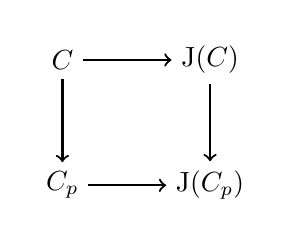
\begin{tikzpicture}
\matrix [column sep=10mm,row sep=10mm]
{
\node (C) {$C$}; & \node (JC) {J($C$)}; \\
\node (Cp) {$C_p$}; & \node (JCp) {J($C_p$)}; \\
};
\draw [thick, ->] (C) -- (JC);
\draw [thick, ->] (Cp) -- (JCp);
\draw [thick, ->] (C) -- (Cp);
\draw [thick, ->] (JC) -- (JCp);
\end{tikzpicture}
\end{center}

The objects on the left are algebraic curves; the objects on the right
are Abelian varieties.  The horizontal arrows correspond to constructing
a curve's associated Jacobian variety; the vertical arrows correspond
to reduction modulo a prime.

At the end of the previous chapter, we were working on the lower-left
half of this diagram.  We reduced a curve modulo a prime, then computed
the order of various divisors on the reduced curve, which essentially
computes orders of points on the reduced curve's Jacobian variety.
We now wish to show that those group orders are the same as if we
had constructed the Jacobian of the original curve and then reduced
the Jacobian modulo the prime.

\item Study the effects of reduction modulo a prime on an Abelian variety.

At this point, we no longer need any special properties of the
Jacobian variety; it suffices to study how reduction modulo a prime
affects the group structure on an Abelian variety.  In particular, we
will find that the factor of an element's order coprime to the
reduction prime is preserved.

\end{enumerate}

\section{The Riemann-Roch Theorem}

The Riemann-Roch Theorem is one of the most celebrated theorems in
mathematics.  Not only does it provide a crucial tool in understanding
the structure of algebraic extensions, but it does so by tying
together algebra, analysis, and geometry in one equation.

First, let's review that equation:

\theorem {\rm (Riemann-Roch)}

% For any divisor $\mathfrak{b}$,
% 
% $$l(\mathfrak{b}) = \deg \mathfrak{b} + 1 - g + l(\mathfrak{c}-\mathfrak{b}) $$
% 
% where $l(\mathfrak{b})$ is the dimension of the vector space
% $L(\mathfrak{b})$ of multiples of $-\mathfrak{b}$, $g$ is the genus of
% the extension, and $\mathfrak{c}$ is any divisor of the canonical class of
% differentials.

For any divisor $\mathfrak{b}$,

% $$l(\mathfrak{b}) = \deg \mathfrak{b} + 1 - g + l(\mathfrak{c}-\mathfrak{b}) $$
% $$l(-\mathfrak{b}) = \deg \mathfrak{b} + 1 - g + l(\mathfrak{b}-\mathfrak{c}) $$
% $$l(\mathfrak{b}) = \deg -\mathfrak{b} + 1 - g + l(-\mathfrak{b}-\mathfrak{c}) $$
% $$l(\mathfrak{b}) = - \deg \mathfrak{b} + 1 - g + l(-\mathfrak{b}-\mathfrak{c}) $$

$$l(\mathfrak{b}) = - \deg \mathfrak{b} + 1 - g + l(-\mathfrak{b}-\mathfrak{c}) $$

where $l(\mathfrak{b})$ is the dimension of the vector space
$L(\mathfrak{b})$ of multiples of $\mathfrak{b}$, $g$ is the genus of
the extension, and $\mathfrak{c}$ is any divisor of the canonical class of
differentials.

\endtheorem

Interrelated by this theorem is the purely algebraic concept of the
dimension of the vector space of multiples of a divisor, the geometric
concept of the genus, and the analytic concept of a differential.

However, this sophistication comes with a price.  Specifically, we
need a topology to define the genus, and we need a limit to define the
differential.

Andr\'e Weil showed how the Riemann-Roch theorem can be stripped of
the analysis and the geometry, and proved as purely a result in
algebra.  The genus, instead of a topological invariant, now appears
as merely a least upper bound on a divisor's degree of specialization,
and a differential becomes an object in a dual space that maps a
function into the field of constants.  The advantage of this
formulation is that does not require any topological structure, and is
therefore well suited to use with finite fields.  It is this
formulation I will now adopt.

First, at any place in the function field, there is a local valuation
ring with a maximal prime ideal.  We can normalize the valuation (it
is discrete) and pick a element of unit valuation to use as a
uniformizing variable.  By multiplying as necessary by some power of
this element, we can adjust any field element to be a unit of the
valuation ring and thus associate an order ${\rm ord}_{\mathfrak{p}}$
with that element.  The valuation ring's units are a finite extension
of the constant subfield; they are the constant subfield if it is
algebraically closed.  By subtracting out the remainder mod
$\mathfrak{p}$, we get an element of higher order, which we can again
subtract out, and so on, building a power series in the uniformizing
variable.  Each element of the function field thus has a power series
associated with it at each place $\mathfrak{p}$.

A collection of such power series, one at each place, with arbitrary
coefficients except that there are only a finite number of
coefficients with negative powers, is called a {\it vector}.  Each
individual power series is called a {\it component} of the vector.
Clearly, every function has a vector associated with it; but the
converse is not necessarily true.  The mapping from functions to
vectors is injective, though.  Any two different functions will have a
non-zero difference that must therefore have a finite value, of finite
order, at some place $\mathfrak{p}$, and their vectors will differ at
that point.

We also have a dual space of {\it covectors}.  The coefficients of a
covector component at a place are dual to the constant field at that
place; if the constant field is algebraically closed, then the
covector coefficients are in the constant field.  Like vectors,
covectors can only have a finite number of negative power
coefficients.

We define a dot product between a vector $v$ and a covector $\lambda$:

$$ v \cdot \lambda = \sum_{\mathfrak{p}} \sum_{i+j=-1} v_{\mathfrak{p},i}
  \lambda_{\mathfrak{p},j} $$

where $v_{\mathfrak{p},i}$ is the coefficient of the $i^{\rm th}$
power in $v$'s component at $\mathfrak{p}$, and likewise for
$\lambda_{\mathfrak{p},j}$.  Notice that the second summation requires
at least one of $i$ or $j$ to be negative, so there will only be a
finite number of places for the first sum at which the second sum
contributes anything at all.

Weil also requires the {\it Theorem of Independence}, which states
that, although an arbitrary (full) vector may not have a function
associated with it, a function can always be found which matches a set
of finite prefixes at a finite number of places.  This can be
demonstrated using Theorem \ref{finite orders construction},
repeatedly applied a finite number of times.  We also need to know
that a function without a pole is constant.

With this setup, we can now prove a series of theorems that lead up
the the Riemann-Roch Theorem.

\theorem

$$l(\mathfrak{p}) \leq \deg \mathfrak{p} +1$$

i.e, $l(\mathfrak{p})$, the dimension (over the constants) of
$L(\mathfrak{p})$, the multiples of $-\mathfrak{p}$, is no more than
the degree of the divisor $\mathfrak{p}$, plus one.

\proof

Since $\deg -\mathfrak{p} = - \deg \mathfrak{p}$, there are at least
$\deg \mathfrak{p}$ poles (counting multiplicities) in
$-\mathfrak{p}$, and at least $\deg \mathfrak{p}$
coefficients with negative powers in the vectors corresponding
to the elements in $L(\mathfrak{p})$

.  We can impose

\endtheorem

\theorem

If $\mathfrak{A}$ is divisible by $\mathfrak{B}$, i.e, if
$\mathfrak{A}\mathfrak{B}^{-1} \subseteq {\cal I}$, then

$$n(\mathfrak{A}) - l(\mathfrak{A}) \leq n(\mathfrak{B}) - l(\mathfrak{B}) $$

$$n(\mathfrak{p}) \equiv {\rm deg} \mathfrak{p}$$

\proof

Consider $\mathfrak{C} = \mathfrak{A}\mathfrak{B}^{-1}$.
Now $n(\mathfrak{C}) = n(\mathfrak{A}) - n(\mathfrak{B})$ and since
$\deg -\mathfrak{C} = - \deg \mathfrak{C}$, and
$\mathfrak{C}$ is integral (by supposition),
there are exactly
$n(\mathfrak{C})$ poles (counting multiplicities) in $-\mathfrak{C}$.
, and at least $\deg \mathfrak{p}$
coefficients with negative powers in the vectors corresponding
to the elements in $L(\mathfrak{p})$

.  We can impose

\endtheorem

Back to the Riemann-Roch Theorem...

It immediately follows (from $\mathfrak{b}={\bf 0}$) that
$l(\mathfrak{c})=g$, which can be taken as the definition of the
genus.

We can now pick $g$ independent differentials from $\mathfrak{c}$ and
use them (along with an arbitrary origin) to map into the torus
${\bf C}/\Lambda^g$.

Now, Abel's Theorem and the Jacobi inversion theorem ([Griffiths and
Harris], p. 235) shows that ${\rm Pic}^0$, the group of divisors of
degree zero modulo linear equivalence is isomorphic to ${\bf
C}/\Lambda^g$.

Alternately, ([Lang], II, \S1, Theorem 3), we can factor a mapping
of a product into an abelian variety into mappings on each factor.

Lang also characterizes Abel's theorem as follows:

\begin{quote}

Let $\omega_1, ..., \omega_g$ be a basis for the differential forms
on the first kind of V.  If $\mathfrak{a} = \sum n_i P_i$ is a
[divisor] of degree 0 on V, and P is a fixed point of V, then
the map into ${\bf C}/\Lambda^g$ given by:

$$\mathfrak{a} \to \sum n_i (\int_P^{P_i}\omega_1, ..., \int_P^{P_i}\omega_g)$$

is well defined modulo the periods... the kernel consists of those
divisors that are linearly equivalent to 0 (i.e, principal); this is
Abel's theorem.

\end{quote}


\section{Jacobian Varieties}

An algebraic extension is a simple example of what algebraic geometers
term a {\it variety}, which is the zero locus of a set of polynomials
defined over some field.  Thus, for example, the unit circle is a
variety (defined over the real numbers), because it is the zero locus
of $x^2+y^2=1$.  But the points $(1,0)$ and $(-1,0)$ are also a
variety, because they are the zero locus of the {\it set} of
polynomials $\{x^2=1; y=0\}$.

An {\it abelian variety} is a variety accompanied by a commutative
group structure on its elements, which typically includes picking an
arbitrary zero point as the identity element.  The circle is an
abelian variety, if we identify its points with their angles from the
x-axis and make $(1,0)$ our identity element.  Now any two points can
be ``added'' or ``subtracted'' (by adding or subtracting their
respective angles) to obtain a third point, and each point has an
inverse associated with it (its mirror image across the x-axis).  It
should be obvious that the choice of a zero point was totally
arbitrary.  Likewise, the points ${(1,0), (-1,0)}$ also form an
abelian variety; their group structure is isomorphic to ${\bf Z}_2$ and
the choice of one of them as the identity is, again, arbitrary.

Is every variety abelian?  No, but any complete, non-singular variety
can be homomorphicly mapped into an associated abelian variety
(typically of higher dimension), called its {\it Jacobian variety}.
This fact, combined with the extensive body of literature on abelian
varieties ([Mumford], [Birkenhake and Lange], [Lang], to mention a
few), makes the Jacobian variety an important object of study (though
David Mumford, in the preface to [Mumford], described it as a
``crutch'').

We will be needing only a tiny bit of this theory here, so my goal in
this section is only to demonstrate how the Riemann-Roch Theorem
allows us to set up an abelian group structures on an algebraic
extension.

\section{Endomorphism Rings}

Any commutative group $G$ induces a (non-commutative) ring structure
on its endmorphisms, defined as follows (remember that an
endomorphism is a homomorphism from an object to itself):

Two endmorphisms $\phi(g): G \to G$ and $\gamma(g): G \to G$ are added
using $G$'s group operation on the images: $(\phi+\gamma)(g) =
\phi(g)\cdot\gamma(g)$, where $\cdot$ denotes the group operation.
The additive identify is the endmorphism that maps the entire group
onto its identity element.

Two endmorphisms $\phi(g): G \to G$ and $\gamma(g): G \to G$ are
multiplied using composition of mappings: $(\phi\gamma)(g) =
\phi(\gamma(g))$.  The multiplicative identity is the endmorphism that
maps every element in the group onto itself.

Let us now verify that these operations define a ring, the {\it endomorphism
ring} of G, which we shall denote ${\rm End}(G)$.  The properties
of the identity elements are fairly obvious, I think.  Almost as
obvious is that the associative and commutative properties of the
underlying group translate directly into additive associative and
commutative properties in the endmorphism ring.  The multiplicative
properties follow from composition of mappings being associative, but
not necessarily commutative.  The distributive law follows from the
easily verified identity $\phi(\gamma(g)\cdot\mu(g)) = \phi(\gamma(g)) \cdot
\phi(\mu(g))$, using the fact that $\phi$ is an endomorphism, and thus
a homomorphism, and therefore maps the group operator through.

The ring of integers ${\bf Z}$ can be mapped homomorphicaly\footnote{An easy
consequence of ${\bf Z}$'s repelling universal property in the category of
rings, see [Lang], p. ?} into any ring, and an endomorphism ring is no
exception.  We'll denote by $[m]$ the endmorphism mapped to by the
integer $m$. $[0]$ is clearly the additive identity mapping all
elements to the group identity.  $[1]$ is, of course, the
multiplicative identity mapping all elements to themselves.  $[2]$ is
$[1]+[1]$, the endmorphism that composes each element with itself
(using the group operator): $[2]: g \to g\cdot g$.  $[3]$ composes
each element with itself thrice: $[3]: g \to g\cdot g\cdot g$, etc.

Because ${\bf Z}$ is commutative, the subring $[m]$ it maps to is also
commutative, even though ${\rm End}(G)$ may not be.



\section{Good Reduction}

My notes from [Sh61].

{\small\begin{verbatim}

A function (Y -> k) is regular at a point on a variety if there exists
an open neighborhood of the point where the function is given by a
rational function of polynomials, the denominator never zero.
(relation to coordinate ring?)

A map (Y -> k) is regular on Y if it is regular at every point of Y.

A morphism (X -> Y) between varieties is a continuous map (in the
Zariski topology) such that pullbacks of regular functions are
regular.

A rational map is a morphism defined only on an open subset.

Given a rational map from affine varieties X to Y, if [x,y,z] is Y's
coordinate system, then we pullback to a regular function, which is a
rational function in X's function field.  So Y's coordinates are given
by rational functions in X's coordinates.

A group variety is an algebraic variety equipped with a group
structure, where the group operation and group inversion are rational
maps.  If the group operation is commutative, it's an abelian variety.

A homomorphism between abelian varieties is a rational map that
commutes with the group operation.

An endomorphism is a homomorphism from the variety to itself.

Endomorphisms of a group form a ring.  Addition is performed by
mapping through both endomorphisms, then applying the group operation,
which is commutative, so endomorphism addition is commutative.
Multiplication is performed by composition, and need not be
commutative.

Using just the addition structure, we get an abelian group that can be
structued as a Z-module.  Multiplication by an integer is just
repeated application of the endomorphism.

We can promote the endomorphism ring into an algebra by tensoring with
Q, call this EndQ(A).  Elements of EndQ(A) are basically endomorphisms
with an associated 1/n denominator (numerators can be sucked into the
endomorphism).

A lattice is a free Z-module of the same rank as the algebra over Q.

An order is a lattice that is also a subring and contains the identity.

The order of A, written t, is the image of the endomorphism ring in
the endomorphism algebra.

a is a lattice in the endomorphism algebra contained in t, so it's a
collection of actual endomorphisms.

g(a,A) is the set of points on A mapped to 0 by every element of a.

Prop 16. Let a be an integral ideal (p. 49) of F.  Reduction mod p
defines a homomorphism of g(a,A) onto g(a,A^).  If a is prime to the
characteristic of k^, this homomorphism is an isomorphism.


Div(C) is group of divisors
Div0(C) is group of degree 0 divisors
P(C) is group of principal divisors

P(C) in Div0(C) in Div(C)

define Pic(C) = Div(C)/P(C)
define Pic0(C) = Div0(C)/P(C)

Pic0(C) is isomorphic to the Jacobian variety with a point O.

Given a degree zero divisor in Div0(C), we can use the group law on
the Jacobian to construct a single point corresponding to the divisor.
Asking if the divisor is principal is asking if this point is O.
Asking if any multiple of the divisor is principal is asking if any
multiple of this point is O.

We can define an endomorphism to be addition by a point, using the
group law.  NO - doesn't take identity to identity.

Let's consider [n], the endomorphism defined by applying the group
operation n times (n is an integer).  This should generate a lattice
contained in t, so it's an integral ideal.  g([n], A) is the set of
points whose n-multiples are principal.

Given a divisor whose (k p^q)-multiple is principal, let's multiply by
p^q and get a divisor whose k-multiple is principal.  Endomorphism
ideal [k] is prime to p.  Then this divisor point will be in g(a,A)
and g(a,A^), where a is [k].

We can determine that the divisor point is in g(a,A^) for a=[k] by
determining that the divisor's k-multiple is principal on the module
curve.  Since this is an isomorphism, the divisor point is also in
g(a,A) for a=[k].




Given a non-singular algebraic curve C, we reduce mod p to get Cp.
Good reduction implies that Cp is non-singular with the same genus.  C
has an associated Jacobian J.  Cp also has an associated Jacobian Jp.

PROBLEM: (hopefully) Show that J mod p is Jp.

Construct J as follows.  Pick r > 2g-2.  Symmetric group J^(r).  Pick
r-g extra points and find an open covering of J^(r).  Within each
open set, construct J locally.

\end{verbatim}
}


\mychapter{Algebraic Extensions}

{\bf THIS CHAPTER IS VERY VAGUE AND INCOMPLETE.}

We now turn to the algebraic extension in general.  Theorem ? allows
us to collapse any two adjacent algebraic extensions together, so we
need only consider an algebraic extension over a transcendental
extension.  The most basic case, the one that we've studied in the
last two chapters, is when the integrand involves only polynomials and
a single root, so we are integrating on an algebraic curve and our
algebraic extension occurs directly over the variable of integration:
${\bf C}(x,y)$.  However, many of these results are applicable in the
more general case where we have a series of field extensions that end
in a transcendental (exponential or logarithmic) extension followed by
an algebraic extension.  I'll use the notation ${\rm K}(\theta, y)$ to
emphasize when this is the case.

\mysection{Integral Elements}

\definition

An element $f \in {\rm K}(\theta,y)$ is {\bf integral} if it satisfies a
monic polynomial with coefficients in ${\rm K}[\theta]$.

\enddefinition

Intuitively, an integral element is one with no finite poles.
To see this, at least in the case where $K = {\bf C}$, define
$z = {1 \over f}$ and substitute this into $f$'s monic polynomial:

	$$f^n + a_{n-1} f^{n-1} + \cdots + a_1 f + a_0 = 0$$

	$$z^{-n} + a_{n-1} z^{-n+1} + \cdots + a_1 z^{-1} + a_0 = 0$$

	$$1 + a_{n-1} z + \cdots + a_1 z^{n-1} + a_0 z^n = 0$$

Now, if $z$ is zero at a place $p$ over $x=x_0$, at least one of this
polynomial's roots must be zero at $x=x_0$.  Since all of the $a_i$
are finite at $x=x_0$ (they are polynomials), multiplying any of them
by zero yields zero, so substituting in $z=0$ yields $1=0$. We
conclude that $z$ can not be zero, and thus $f$ can not have a pole
over $p$.

What's special about infinity?  Why not exclude some other place?
Well, nothing's all that special about infinity.  We've already seen
how a birational transformation can be used to swap infinity with any
finite point.  Demanding that a field element have no poles anywhere
is too restrictive, because Theorem ? tells us that such an element
must be constant.  So we want to relax this requirement slightly by
allowing poles over a single point.  We use infinity because it's
convenient.

It's not always obvious from inspection which functions are integral.
Something like $y \over x$, which appears to have a pole at $x=0$, is
actually integral if, for example, $y^2=x^3$.  Then we can consider
squaring $y \over x$ to obtain ${y^2 \over x^2} = {x^3 \over x^2} =
x$.  If the square is finite, then the original function had to be
finite (you can't square infinity and get a finite value), so we
conclude that $y \over x$ is, in fact, globally integral in ${\bf
C}(x,y); y^2=x^3$, as it satisfies the monic polynomial $f^2 - x = 0$.

Unfortunately, we have no straightforward means to construct such a
polynomial, or prove that one doesn't exist, for any particular
function $f$.  To test a function to determine if it is integral,
we'll need a more advanced approach.

%\definition
%
%A field's {\bf local ring} at a place $p$ is the set of
%all functions in the field with no pole at $p$; that
%is, $ \lim_{x\to p} f(x) \ne \infty $.
%
%A function is {\bf locally integral} at a place $p$
%if it belongs to its field's local ring at $p$.
%
%\enddefinition
%
%Remember the distinction I drew between a {\it pole} and a {\it
%removable singularity} is Chapter ?.  That's the reason for the limit
%in the definition; removable singularities are specifically included
%in a local ring.  Thus, $x\over\sqrt{x}$ is locally integral at $x=0$,
%despite the fact that it has a zero denominator, because
%$\lim_{x\to0}{x\over\sqrt{x}}=\sqrt{x}=0$, a finite value.
%
%It is often important, however, to specify which field we are
%refering to when we discuss a local ring.
%
%\example \quad
%
%In the field ${\cal C}(x)$, the function $x$ is locally integral at $x=0$.
%
%In the field $F = {{\cal C}(x,y); y^2=x+1}$, the function $x$ is locally integral
%at both $(x=0, y=1)$ and $(x=0, y=-1)$.  There is no place $x=0$ in
%this field; to speak of it so is ambiguous, as there are two places
%in $F$ where $x=0$.
%
%Likewise, $y$ is locally integral in $F$ at both $(x=0, y=1)$ and
%$(x=0, y=-1)$.  It is not locally integral in ${\cal C}(x)$ at $x=0$ simply
%because $y$ does not exist in the field ${\cal C}(x)$.
%
%\endexample
%
%Thus, a function like $x$ can be locally integral in both ${\cal C}(x)$ and
%${\cal C}(x,y)$; it is important to specify which we are talking about.
%
%Since the fields ${\cal C}(x)$ and ${\cal C}(x,y)$ are distinct, and have different
%places, they also have different local rings.  There is an important
%connection between them, however.
%
%\theorem
%\label{local integral polynomial}
%
%A function $f$ is locally integral at a place $p$ in ${\cal C}(x,y)$ if it
%satisfies a monic polynomial with coefficients in the local ring of
%${\cal C}(x)$ at the corresponding place in that field.
%
%\proof
%
%
%\endtheorem
%
%The converse is not true; just because a function does not satisfy
%such a monic polynomial does not mean that it is not locally integral.
%A slightly weaker converse does hold, however:
%
%\theorem
%
%A function $f$ in ${\cal C}(x,y)$ which is locally integral at all
%places in ${\cal C}(x,y)$ over a place $p$ in ${\cal C}(x)$ satisfies
%a monic polynomial with coefficients in the local ring of ${\cal C}(x)$
%under $p$.
%
%\proof
%
%Construct the polynomial
%
%$$(z - f(x,y))(z - f(x,y_2)) \cdots (z - f(x,y_n)) = 0$$
%
%$f$ clearly satisfies this polynomial at every place over $p$.
%Furthermore, multiplying out the terms yields:
%
%$$\matrix{z^n & - (f(x,y)+f(x,y_2)+\cdots+f(x,y_n)) z^{n-1} \hfill\cr
%   & + \quad (f(x,y)f(x,y_2)+f(x,y)f(x,y_3)+\cdots+f(x,y_{n-1})f(x,y_n)) z^{n-2} \hfill\cr
%   & + \cdots + f(x,y)f(x,y_2)\cdots f(x,y_n) = 0 \hfill\cr}$$
%
%All of these coefficients are symmetric functions in $y_i$, and thus
%exist in ${\cal C}(x)$.  Furthermore, since $f$ is finite (by
%assumption) at all conjugate values over $p$, each of these
%coefficients must also be finite at $p$ (since they are constructed by
%addition and multiplication from the conjugate values of $f$), and are
%thus in the local ring of ${\cal C}(x)$ at $p$.
%
%\endtheorem
%
%In short, a function in ${\cal C}(x,y)$ which satisfies a monic
%polynomial whose coefficients are in a local ring of ${\cal C}(x)$ at
%a point $p$ is locally integral in ${\cal C}(x,y)$ at all places over
%$p$.  A function which does not satisfy such a polynomial has
%a pole at at least one place over $p$.
%
%A more advanced, more purely algebraic approach to this subject would
%{\it define} local rings using Theorem \ref{local integral
%polynomial}, then use valuations and completions to {\it prove} the
%connection between local rings and poles (or the lack thereof).  See
%[van der Waerden], Chapter 18.  I will forego this in favor of this
%simpler, more analytic (note the use of the limit) approach.
%
%
%Having established the existence and basic properties of {\it locally}
%integral elements, we can now discuss {\it globally} integral
%elements.  Obviously, elements in a field will be locally integral at
%more than one place.  In fact, field elements will be locally integral
%at almost all places (because they only have a finite number of
%poles).  So, intuitively, a {\it globally} integral element would be
%one that is integral at every place in a field.  However, Theorem ?
%immediately tell us that the only such functions (those which have no
%poles anywhere) are the constants, so this turns out to be too
%restrictive to be useful.  Instead, we exclude infinity and define:
%
%\definition
%
%A function is {\bf globally integral} in a field if it is locally
%integral at all {\it finite} places in the field.
%
%\enddefinition
%
%
%We could use Theorem \ref{local integral polynomial} and the fact
%that, in ${\cal C}(x,y); y^2=x^3$,
%
%	$$ \left({y \over x}\right)^2 - x = 0 $$
%
%to conclude that, since this is a monic polynomial with coefficients
%globally integral in ${\cal C}(x)$, $y \over x$ must be globally
%integral in ${\cal C}(x,y); y^2=x^3$.  Theorem \ref{local integral
%polynomial} can be easily generalized:
%
%\theorem
%
%A function $f$ is globally integral in ${\cal C}(x,y)$ if it
%satisfies a monic polynomial with globally integral coefficients in
%${\cal C}(x)$.
%
%\proof
%
%\endtheorem
%
%Proof that globally integral elements form a finite extension:
%[Eichler], p. 54
%
%Proof that field elements are determined by their divisors, up to a
%constant multiple: [Eicher], p. 84
%
%[Eicher], p. 86: Prime divisors are isomorphic with special local rings.
%

\mysection{Modules}

We'll resort now to {\it modules}, a fairly important algebra concept
backed by a substantial body of theory, upon which I shall only draw
as needed.  General references include [Atiyah+McDonald] and [Lang].

\definition

An {\it R-module} over a ring R is an additive group M acted on by R
(i.e, there is a mapping $R \times M \to M$) in a distributive manner:

$$(r_1 + r_2)m = r_1 m + r_2 m \qquad r_1, r_2 \in {\rm R};\, m \in {\rm M}$$

where we have adopted the usual convention of writing R's action on M
as a multiplication.

\enddefinition

\definition

A {\it free R-module} is an R-module spanned by a linearly independent basis
$\{b_1, b_2, ... b_n\}$.  It consists of all elements formed as follows:
\footnote{I'll also note that a multiplication rule needs to be specified
between the basis elements and the elements of the ring, and an
addition rule between the elements of the module.  Also,
the expression has to be {\it unique} --- you can't be
able to write an element two different ways.  In our
case, these rules are obvious, but that's not always the case.}

	$$ a_1 b_1 + a_2 b_2 + ... + a_n b_n; \qquad a_i \in R $$


\enddefinition

Not all modules have a finite set of generators, and not all those
have a linearly independent set of generators.  Elements formed from a
basis can be added by using the module's distributive property to
factor out the coefficients from of each basis element and then
performing the addition in the ring R:

$$ (a_1 b_1 + a_2 b_2 + ... + a_n b_n) + (c_1 b_1 + c_2 b_2 + ... + c_n b_n) $$
$$  = (a_1 + c_1) b_1 + (a_2 + c_2) b_2 + ... + (a_n + c_n) b_n $$

So the elements generated from a basis clearly form a module.  R operates
on them by multiplication by every coefficient.

\example \quad
\label{sample modules}

An ideal I in a ring R is a R-module, but a subring S of R, in
general, is not, because multiplication by an element of R might not
produce a result in the subring.  R, however, can always be viewed as
an S-module.

% XXX
% If R is a principal ideal ring, then every ideal is also a
% free R-module, admitting a basis consisting of a single
% element, a generator of the ideal.
%
% Is this true?  Any zero divisor counterexamples?

\endexample


Note that it is vitally important to specify the ring used for the
coefficients.  For example, consider the basis $\{1, y\}$.  Treating
this as a ${\bf C}(x)$-module, I can form ${y \over x} = {1 \over x}
y$, since ${1 \over x} \in {\bf C}(x)$.  However, $y \over x$ does
{\it not} belong to the ${\bf C}[x]$-module generated by $\{1, y\}$.
I would need to use polynomial coefficients to form a ${\bf
C}[x]$-module, not the rational functions coefficients allowed in a
${\bf C}(x)$-module.  We'll be primarily interested in ${\rm
K}[\theta]$-modules, ${\rm K}(\theta)$-modules, and ${\cal
I}$-modules, where ${\cal I}$ is the ring of integral elements in
${\rm K}(\theta,y)$.


% \vfil\eject
% \mysection doesn't work because of the math in the section title
\section{The ${\rm K}[\theta]$-module ${\cal I}$}

Since polynomials have no finite poles, they are integral elements,
and thus ${\rm K}[\theta] \subseteq {\cal I}$.  Thus, ${\cal I}$ (the
ring of integral elements) is trivially a ${\rm K}[\theta]$-module
(see Example \ref{sample modules}), but what is not nearly so obvious
is that it is also a free module, a fact which underlies a great deal
of our theory.  I'll prove this first by showing that ${\cal I}$ is
finitely generated as a ${\rm K}[\theta]$-module, then showing the
existance of a linearly independent set of generators.

Let's start with a preliminary theorem.

\theorem
\label{construction of dual basis}

If $\{w_1,\ldots,w_n\}$ is a basis for a finite separable field
extension $E/K$, then a dual basis $\{u_1,\ldots,u_n\}$ can be
constructed such that ${\rm Tr}(w_i u_j) = \delta_{ij}$.
([Lang] Corollary VI.5.3)

\proof

Consider the following matrix:

$$M = \begin{pmatrix}{\rm Tr}(w_1 w_1) & & \cr \vdots & \ddots & \cr {\rm Tr}(w_1 w_n) & \cdots & {\rm Tr}(w_n w_n)\end{pmatrix}$$

Now take an element $x \in E$, and represent it relative to the basis
$\{w_1,\ldots,w_n\}$ as a row vector $X = (x_i)$.  Multiplying $X M$
produces a row vector whose $j^{\rm th}$ element can be written:

$$\sum_i x_i {\rm Tr}(w_j w_i) = {\rm Tr}(w_j \sum_i x_i w_i) = {\rm Tr}(w_j x) = {\rm Tr}_x(w_j)$$

where I used first the $K$-linearity and additive distributive
properties of ${\rm Tr}$, then wrote ${\rm Tr}_x: f(a) = {\rm Tr}(ax)$
to emphasize that I'm regarding ${\rm Tr}_x$ as a linear form in ${\rm
Hom}_E(E,K)$.  So, if $M$ is singular, then there exists some non-zero
element $x$ such that ${\rm Tr}_x$ is zero for all of $w_i$, which
form a basis set, so ${\rm Tr}_x$ must therefore be the zero map.
This can only happen if ${\rm Tr}$ is identically zero, which would be
the case for an inseparable extension.  For the separable case,
therefore, $M$ must be invertible, and we can write:

$$M^{-1} M = \begin{pmatrix}1 & & \cr & \ddots & \cr & & 1\end{pmatrix}$$

A moment's thought now shows that the rows of $M^{-1}$ are the desired
dual basis elements, written with respect to $\{w_1,\ldots,w_n\}$.

\endtheorem

% \vfil\eject

\theorem
\label{I is finitely generated}

${\cal I}$ is a finitely generated ${\rm K}[\theta]$-module.
([A+MacD] Proposition 5.17; [Lang] Exercise VII.3)

\proof

Regarding ${\rm K}(\theta,y)$ as a vector space over ${\rm
K}(\theta)$, we can easily construct a basis of integral elements by
starting with $\{1, y, \ldots, y^{n-1}\}$ and multiplying each element
(if needed) by a polynomial in $\theta$ which cancels all of its poles:

$${\rm K}(\theta,y) = {\rm K}(\theta)\{w_1,\ldots,w_n\} \qquad \forall i(w_i \in {\cal I})$$

Using Theorem \ref{construction of dual basis}, construct a dual basis
$\{u_1,\ldots,u_n\}$ so that ${\rm Tr}(w_i u_j) = \delta_{ij}$.  Take
any $x \in {\cal I}$ and write it using the dual basis:

$$x = \sum_i a_i u_i \qquad a_i \in {\rm K}(x)$$

Now consider ${\rm Tr}(x w_j)$.  Now, $x$ and $w_j$ are both in ${\cal
I}$, so $x w_j$ is in ${\cal I}$, and therefore has a monic minimum
polynomial with coefficients in ${\rm K}[\theta]$.  Since ${\rm Tr}$ equals
some integer multiple of the negative of the second coefficient in a
monic minimum polynomial, ${\rm Tr}(x w_j) \in {\rm K}[\theta]$.  But also,

$${\rm Tr}(x w_j) = {\rm Tr}(\sum_i a_i u_i w_j)
 = \sum_i {\rm Tr}(a_i u_i w_j) %\hfil (Tr an additive homomorphism)
 = \sum_i a_i {\rm Tr}(u_i w_j) %\hfil (linearity of Tr)
 = a_i$$

which establishes that $\forall i (a_i \in {\rm K}[\theta])$, so

$${\cal I} \subseteq {\rm K}[x]\{u_1,\ldots,u_n\} $$

${\rm K}[\theta]$ is a Noetherian ring (Theorem ??), so ${\rm
K}[\theta]\{u_1,\ldots,u_n\}$ is a Noetherian module (Theorem ??),
which means that ${\cal I}$, as a submodule, is Noetherian
and thus finitely generated (Theorem ??).

\endtheorem

% \vfil\eject

\theorem
\label{submodules of free modules over PIRs are free}

Any submodule of a finite free module over a principal ideal ring is free.
([Lang] Theorem III.7.1)

\proof

Let $F = R\{w_1,\ldots,w_n\}$ be a free $R$-module ($R$ a principal
ideal ring) with a submodule $M$.  Consider $F_i =
R\{w_1,\ldots,w_i\}$, the free $R$-module generated by the first $i$
basis elements, and $M_i = F_i \cap M$.  We will show inductively that
all of the $M_i$ are free $R$-modules, and since $F_i = F$ and $M_i =
M$, this will prove the theorem.

First, consider $M_1 = R\{w_1\} \cap M$.  If $M_1$ is not empty (and
thus free), then any $m \in M_1$ can be written $r w_1$.  Since a
module forms an additive group, and we can operate on the module using
all the elements of $R$, it follows that all the $r$'s must form an
ideal, and since $R$ is principal, that ideal can be written with a
single generator, say $(r_1)$, and $M_1 = R\{r_1 w_1\}$ (or is empty).

Now, assume that $M_j$ is free for all $j<i$.  Consider all $x \in
M_i$, which can be written $r_1 w_1 + \cdots + r_i w_i$.  Either $M_i
= M_{i-1}$ (and is therefore free), or at least some of the $r_i$ are
non-zero.  By the same rationale as the last paragraph, these $r_i$
form an ideal, which can be written $(r_i)$.  Take any element $x \in
M_i$ with its $i^{\rm th}$ coefficient $r_i$ and add it to
$M_{i-1}$'s basis set to form a basis set for $M_i$, since some
multiple of this element can be used to cancel any $i^{\rm th}$
coefficient from an element in $M_i$ and leave an element in $M_{i-1}$
which can be formed using the remaining basis elements.

\endtheorem

A {\it torsion-free} module has no ``zero divisors'', in the sense
that no non-zero element of its associated ring can operate on a
non-zero element of the module and produce zero.  Since fields are
torsion-free, and all of our modules are subsets of the field
${\rm K}(\theta,y)$, they are all torsion-free.

\theorem
\label{finitely generated torsion-free modules over a PIR are free}

Any finitely generated, torsion-free module $M$ over a principal ideal
ring $R$ is free. ([Lang] Theorem III.7.3)

\proof

Take a maximal set of $M$'s linearly independent generators $\{w_1,
\ldots, w_n\}$ and any remaining generators $\{y_{n+1}, \ldots,
y_m\}$.  Every $y_i$ is therefore linearly dependant on $\{w_1,
\ldots, w_n\}$:

$$a_i y_i + r_1 w_1 + \cdots + r_n w_n = 0 \qquad a_i \ne 0$$

Take the product of all the $a_i$'s: $a = a_{n+1} a_{n+2} \cdots a_m$
and consider the mapping $x \mapsto ax$ which is injective, since $a
\ne 0$ and the module is torsion-free, so therefore maps $M$ to $aM$,
an isomorphic image which is a submodule of the free module
$R\{w_1,\ldots,w_n\}$.  By Theorem \ref{submodules of free modules
over PIRs are free}, $aM$ is therefore free, and since it is
isomorphic to $M$, we can take a basis of $aM$, divide all of its
basis elements by $a$ (they are all multiples of $a$), and obtain
a basis for $M$.

\endtheorem

Now, since ${\rm K}[\theta]$ is a principal ideal ring (Theorem ??),
Theorems \ref{I is finitely generated} and \ref{finitely generated
torsion-free modules over a PIR are free} demonstrate that ${\cal I}$
is a free ${\rm K}[\theta]$-module.

\definition

A basis for ${\cal I}$ will be called an {\bf integral basis}.

\enddefinition

\theorem

Any integral basis is also a basis for the ${\rm K}(\theta,y)$ field as a
${\rm K}(\theta)$-module.

\endtheorem

While the preceding theorems offer an existance proof for an integral
basis, it is not immediately clear how to obtain one for any
particular field, and in fact the calculation of an integral basis
ultimately becomes one of the biggest computational barriers in this
theory.  Therefore, I will defer a more detailed discussion until a
later chapter, and instead present a simple construction for the
special case of a simple radical extension.

%\definition
%
%A basis is said to be a {\bf locally integral basis} at a place $p$ in
%${\cal C}(x)$ if the basis elements are locally integral at all places
%in ${\cal C}(x,y)$ over $p$ and the determinant of its conjugate
%matrix assumes a finite, non-zero value at that place.
%
%\enddefinition
%
%\theorem
%
%A function $f$ in ${\cal C}(x,y)$ has no poles over a place $p$ in
%${\cal C}(x)$ iff $f$ can be formed from a basis locally integral at
%$p$, using elements from ${\cal C}(x)$ locally integral at $p$.
%
%\endtheorem
%
%
%With a local integral basis (no pole at a place), there are 1-to-1
%correspondances:
%
%	use coeffs in K(x) w/ no pole at place <=> elem in K(x,y) w/ no pole
%
%	use coeff w/ pole at place <=> elem in K(x,y) w/ pole at place

\mysection{Basis for all Rational Functions}

The first kind of basis we're interested in, a {\it basis for all
rational functions}, is one than spans the entire ${\cal C}(x,y)$ field
as a ${\cal C}(x)$-module.
In other words, we're looking for a basis $\{b_1, b_2,
... b_n\}$ so that everything in ${\cal C}(x,y)$ can be expressed
in the form:

	$$ a_1 b_1 + a_2 b_2 + ... + a_n b_n; a_i \in {\cal C}(x) $$

Such a basis will always have $n$ elements, where $n$ is the degree of
the ${\cal C}(x,y)$ extension over ${\cal C}(x)$, and can be most
conveniently characterized using its {\it conjugate matrix}:

\definition

The {\bf conjugates} of a rational function $\eta(x,y)$ in ${\bf
C}(x,y)$ are the functions formed by replacing $y$ with its conjugate
values.

The {\bf trace} of a rational function $\eta(x,y)$ is the sum of
its conjugates:

$${\rm T}(\eta(x,y)) = \sum_i \eta(x,y_i)$$

The {\bf norm} of a rational function $\eta(x,y)$ is the product of
its conjugates:

$${\rm N}(\eta(x,y)) = \prod_i \eta(x,y_i)$$

Both the trace and norm, as symmetric functions in $y_1,...,y_n$, are
functions in ${\bf C}(x)$.

The {\bf conjugate matrix} ${\bf M}_\omega$ of $n$ elements $\omega_i$
in ${\cal C}(x,y)$, where $n$ is the degree of ${\cal C}(x,y)$ over
${\cal C}(x)$, is the matrix whose each row consists of the $n$
conjugate values of a single element, and whose $n$ rows are formed in
this way from the $n$ elements.

A set of $n$ elements $\omega_i \in {\bf C}(x,y)$ form a {\bf rational
function basis} for ${\bf C}(x,y)$ if the determinant of their
conjugate matrix is non-zero: $|{\bf M}_\omega| \ne 0$

\enddefinition

\definition

For any function $\eta \in {\bf C}(x,y)$ and any rational function
basis $\omega_i$, the {\bf trace vector}
${\bf T}_{\eta/\omega} = \Big({\rm T}(\eta \omega_i)\Big)$ 
of $\eta$ relative to $\omega$
is formed from the
traces of the $n$ products of $\eta$ with the $n$ functions
$\omega_i$.

The {\bf conjugate vector} ${\bf C}_\eta = (\eta(x,y_i))$ is formed from the
$n$ conjugates of $\eta$.

\enddefinition

\theorem
\label{function is zero if trace vector is zero}

For any function $\eta \in {\bf C}(x,y)$ and any rational function
basis $\omega_i$, if ${\bf T}_{\eta/\omega}$ is the zero vector,
then $\eta$ is zero.

\proof

${\bf T}_{\eta/\omega}$, ${\bf M}_\omega$ and ${\bf C}_\eta$
satisfy the matrix equation

$${\bf T}_{\eta/\omega} = {\bf M}_\omega {\bf C}_\eta$$

since each row of this matrix equation has the form

$$ {\rm T}(\eta \omega_i) = \sum_j \omega_i(x,y_j)\eta(x,y_j) $$

Since ${\bf M}_\omega$ is invertible (since its determinant is
non-zero), if ${\bf T}_{\eta/\omega}$ is identically zero, then so must be
${\bf C}_\eta$, and $\eta$ is the first element in ${\bf C}_\eta$.

\endtheorem

\theorem
\label{|M| != 0 implies C(x) basis}

A rational function basis $\omega_i$ spans ${\bf C}(x,y)$ as
a ${\bf C}(x)$-module. ([Bliss], Theorem 19.1)

\proof

Note that when we multiply ${\bf M}_\omega$ by its transpose ${\bf
M}_\omega^T$, the $ij^{\rm th}$ element of ${\bf M}_\omega{\bf
M}_\omega^T$ is:

$$ \sum_k \omega_i(x, y_k)\omega_j(x, y_k) = {\rm T}(\omega_i \omega_j)$$

Since $|{\bf M}_\omega|$ is non-zero, $|{\bf M}_\omega^T|$ is
non-zero, and $|{\bf M}_\omega{\bf M}_\omega^T|$ is non-zero, so given
any function $\eta \in {\bf C}(x,y)$, we can solve the following
equation for ${\bf R}$:

$${\bf T}_\eta = {\bf M}_\omega {\bf M}_\omega^T {\bf R}$$

each of row of which reads:

$$ {\rm T}(\eta \omega_i) = \sum_j {\rm T}(\omega_i \omega_j) r_j $$

Since both ${\bf T}_\eta$ and ${\bf M}_\omega{\bf M}_\omega^T$ are composed of
nothing but traces, they exist in ${\bf C}(x)$, so ${\bf R}$ must also
exist in ${\bf C}(x)$ and its elements therefore commute with the
trace:

$$ {\rm T}(\eta \omega_i) = \sum_j {\rm T}(r_j \omega_j \omega_i) $$

Since the trace of a sum is the sum of the traces:

$$ {\rm T}(\eta \omega_i) = {\rm T}(\sum_j r_j \omega_j \omega_i) $$
$$ {\rm T}((\eta - \sum_j r_j \omega_j) \omega_i) = 0 $$

which implies that $\eta = \sum_j r_j \omega_j$, by Theorem
\ref{function is zero if trace vector is zero}, and since we've
already shown that the $r_j$ are rational functions in ${\bf C}(x)$,
this proves the theorem.

\endtheorem

Let me illustrate with a simple example.

\example

Consider the basis $\{1, y\}$ over the field ${\cal C}(x,y); y^2=x$.
The conjugate value of $y$ is $-y$ (PROVE THIS), so the conjugate
matrix is:

$$C=\left(\begin{matrix}1&1\cr y&-y\cr\end{matrix}\right)$$

and its determinant:

$$\det C=\left|\begin{matrix}1&1\cr y&-y\cr\end{matrix}\right| = -2y$$

Since $-2y$ is not zero, we conclude that $\{1, y\}$ is a basis
for all rational functions over ${\cal C}(x,y); y^2=x$.

\endexample

Notice that I didn't ask whether $-2y$ was zero at some place in the
field.  The determinant of the conjugate matrix can be zero at certain
places; in fact, often is.  It just can't be {\it identically} zero;
i.e, it can't be zero {\it everywhere}.  If this isn't clear, reread
Theorems \ref{function is zero if trace vector is zero} and \ref{|M|
!= 0 implies C(x) basis}, noting that all the matrices are defined
over the {\it fields} ${\bf C}(x)$ and ${\bf C}(x,y)$, where the only
zero element is 0.


% \vfill\eject
\mysection{Divisors and Integral Modules}

In ${\bf C}(x)$, we were working with the quotient field of a
principal ideal ring, so we could always find a single function to
generate any finitely generated ${\bf C}[x]$-module, simply by putting
all the generators over a common denominator, then taking the
G.C.D. of the numerators.

In ${\rm K}(\theta,y)$, we are no longer working with a principal ideal
ring, so we can't guarantee that any particular ideal can be generated
by a single function, but it turns out that every ideal can be
generated by a {\it pair} of functions.  Our course of attack is first
to construct that pair of functions, then use them to determine if in
fact the ideal is principal.

\definition

An {\bf integral module} (or ${\cal I}$-module) is a module formed
over ${\cal I}$, the ring of integral elements in ${\rm K}(\theta,y)$.

\enddefinition

Since ${\cal I}$ itself can be expressed as a ${\rm K}[\theta]$-module
using an integral basis, any ${\cal I}$-module is also a ${\rm
K}[\theta]$-module.  Not all ${\rm K}[\theta]$-modules are ${\cal
I}$-modules, however, since ${\cal I}$ is typically larger than ${\rm
K}[x]$.

% Existance of an integral basis is demonstrated by Atiyah and MacDonald
% via Propositions 5.17, 6.5, and 6.2.  Van der Waerden proves this on
% pp. 174-175 of volume 2.  That ${\cal I}$ is a free module can be
% proven using Lang's theorem 7.3.

Some authors use the term {\it fractional ideal} to refer to an ${\cal
I}$-module.  I have avoided use of this term for two reasons.  First,
I wish to emphasize the concept of a module.  Second, ${\cal
I}$-modules are not ideals, either in the ring ${\cal I}$ (since they
may contain elements not in ${\cal I}$), nor in the field ${\rm
K}(\theta,y)$, since, as a field, ${\rm K}(\theta,y)$ has only the trivial
ideals.  The term {\it fractional ideal} is used because an ${\cal
I}$-module can be regarded as a fraction of ideals in ${\cal I}$.

\theorem ${\cal I}$ is a Noetherian ring.
\label{I is Noetherian}

\proof

Since ${\rm K}$ is a field, ${\rm K}[\theta]$ is a Noetherian ring by
the Hilbert basis theorem, ${\rm K}[\theta] \subseteq {\cal I}$, and
${\cal I}$ is finitely generated as a ${\rm K}[\theta]$-module, so
${\cal I}$ is a Noetherian ring by [Atiyah+McDonald] Proposition 7.2.

\endtheorem

\theorem
\label{order of norm}
The order of the norm of $f$ at a point $\theta_0$ is the sum of the orders
of $f$ at all places over $\theta_0$.

\endtheorem


\theorem
\label{simple zero construction}

A function can always be constructed with a simple zero at a specified
finite, ordinary place $(\alpha, \beta)$, zero order at an additional
finite set of finite, ordinary places $\Sigma$, and non-negative order
at all other finite places.

\proof

Begin with the function $(x-\alpha)$, which is a uniformizing variable
and thus has a simple zero at $(\alpha, \beta)$.  If none of the other
places in $\Sigma$ have x-value $\alpha$, then we are done, since
$(x-\alpha)$ has no finite poles.

Otherwise, compute $(x-\alpha)\over(y-\beta)$ at all places in
$\Sigma$ that do {\it not} have $y = \beta$.  Select a number
$\gamma$ different from all of these values.  The function $(x-\alpha)
- \gamma (y-\beta)$ has no finite poles and
is non-zero at all places in $\Sigma$, but it may now have a zero of
higher order at $(\alpha, \beta)$.  Consider a series expansion
of $y$ in terms of $(x-\alpha)$:

$$y = \beta + c_1 (x-\alpha) + c_2 (x-\alpha)^2 + \cdots$$

So long as $\gamma$ is also selected different from $c_1$, $(x-\alpha)
- \gamma (y-\beta)$ will have a first order zero at $(\alpha, \beta)$
and meet all requirements of the theorem.  The simplest way to do this
is to pick a value for $\gamma$, use Theorem \ref{order of norm} to
check if the function has a simple zero, and if not, choose a
different value for $\gamma$.

% SINGULARITIES?

\endtheorem

\theorem
\label{simple pole construction}

A function can always be constructed with a simple pole at a specified
finite, ordinary place $(\alpha, \beta)$, zero order at an additional
finite set of finite, ordinary places $\Sigma$, and non-negative order
at all other places.

\proof

Begin with the function:

$$f(\alpha,y)\over(x-\alpha)(y-\beta)$$

where $f(x,y)$ is the minimum polynomial of the algebraic extension.
Note that the division by $(y-\beta)$ will always be exact, since
$f(\alpha, \beta)=0$.  So we have a rational function
$P(y)\over(x-\alpha)$, where $P(y)$ is a polynomial in $y$.  It has a
simple pole at $(\alpha, \beta)$, as can be seen from a series
expansion in $x-\alpha$ (again, a uniformizing variable).  Since the
$y-\beta$ factor has been divided out of $f(\alpha,y)$, the numerator
is non-zero at $(\alpha, \beta)$, so the leading term in the series
expansion involves $(x-\alpha)^{-1}$, and the pole is thus simple.

This function is finite at all other places, which is obvious except
when $x=\alpha$ and $y\ne\beta$, where it takes the form $0\over0$,
so we can expand it using L'H\^opital's rule:

$$\lim_{(x,y)\to p} {{P(y)}\over(x-\alpha)}
  = \lim_{{(x,y)\to p}} {{{dP(y)}\over{dx}}\over{{d(x-\alpha)}\over{dx}}}
  = P'(y) \, {{dy}\over{dx}} $$

where $'$ denotes differentiation with respect to the polynomial's
variable.  $P'(y)$ is a polynomial, and is thus finite where $y$ is
finite, as is ${dy}\over{dx}$ (consider a series expansion of $y$ in
terms of $(x-\alpha)$, since all places in $\Sigma$ are finite and
non-singular).  It follows that the function is at least finite
everywhere except at $(\alpha, \beta)$.

% This function is finite at all other places, which is obvious except
% when $x=\alpha$ and $y\ne\beta$, where it takes the form $0\over0$.
A more algebraic way to prove this is to note that
$f(x,y)$ has a simple zero at every place over $x=\alpha$ (assuming
there are no multiple points over $x=\alpha$), so $P(y)$ will have a
simple zero at every place over $x=\alpha$ except $(\alpha, \beta)$,
which will exactly cancel the simple pole from $(x-\alpha)$.

Now, compute the value of the function at all other places in
$\Sigma$, using either L'H\^opital's rule or Puiseux expansion if some
of these are over $\alpha$.  If the value of the function is non-zero
at all of these places, then we are done.  Otherwise, select a number
$\gamma$ different from all of these values.  The function:

$${f(\alpha,y)\over(x-\alpha)(y-\beta)} - \gamma$$

has the desired properties, since it still has a simple pole at
$(\alpha,\beta)$, has no other poles, and is now non-zero at all
places in $\Sigma$.

We can avoid computing any expansions by picking random values of
$\gamma$, and using Theorem \ref{order of norm} to check for any extra
zeros.  Since only a finite number of $\gamma$ values produce extra
zeros, this process is guaranteed to terminate.

% SINGULARITIES?

\endtheorem

\theorem
\label{finite orders construction}

A function can always be constructed with specified integer orders at
a finite set of finite, non-singular places $\Sigma$ and non-negative
order at all other finite places.

\proof

For each pole or zero, use Theorems \ref{simple zero construction} or
\ref{simple pole construction} to construct a function with a simple
pole or a simple zero at that place, zero order at all other places in
$\Sigma$ and non-negative order at all other finite places.  Raise
each of these function to the integer power that is the order of the
corresponding pole or zero, then multiply them all together.

\endtheorem

\definition

A {\bf finite multiple} of a divisor is a function with order equal to
or greater than that required by the divisor at all {\it finite} places.

\enddefinition

For the remainder of this section, I'll assume that our divisors
involve only finite, ordinary places, which can always be guaranteed
in the case of the integration theory.

\theorem
\label{exact order existance}

For any divisior ${\cal D}$ and any finite, non-singular place
$\mathfrak{p}$, at least one finite multiple of ${\cal D}$ exists with
order at $\mathfrak{p}$ exactly that required by ${\cal D}$.

\proof

Use Theorem \ref{finite orders construction} with the zeros and poles
required by ${\cal D}$, adding $\mathfrak{p}$
to $\Sigma$ if necessary.

\endtheorem

\theorem
\label{divisor-module isomorphism}

There is a one-to-one relationship between finitely generated integral
modules and divisors.  Such a module consists of all finite multiples
of its associated divisor, and the order of a module's divisor at
every finite place is the minimum of the orders of the module's
generators at that place.

\proof

For a given divisor ${\cal D}$, consider the set ${\cal M}({\cal D})$
of all finite multiples of ${\cal D}$.
Now, adding two
elements can not reduce their order at any finite place, nor can
multiplying an element by an integral element $i \in {\cal I}$, so
${\cal M}({\cal D})$ is clearly an ${\cal I}$-module, but it
might not be finitely generated.

Since ${\cal D}$ has only a finite number of poles, we can always
construct a function with order equal or less than that of ${\cal D}$
at all finite places simply by taking the inverse of the polynomial
$r=(x-p_1)^{m_1} \cdots (x-p_n)^{m_n}$ where $p_i$ are the x-coordinates
of the poles in ${\cal D}$ and $m_i$ are their multiplicities.
For any $m \in {\cal M}({\cal D})$, $mr$ is integral, so ${\cal M}({\cal D})
\subseteq {\cal I}\{r^{-1}\}$, where ${\cal I}\{r^{-1}\}$ is the ${\cal I}$-module
generated by $r^{-1}$.  Now, since ${\cal I}\{r^{-1}\}$ is a finitely
generated module over a Noetherian ring (remember Theorem \ref{I is
Noetherian}), ${\cal I}\{r^{-1}\}$ is a Noetherian module by
[Atiyah+McDonald] Proposition 6.5, and ${\cal M}({\cal D})$ must also
be a finitely generated ${\cal I}$-module by [Atiyah+McDonald]
Proposition 6.2.

Let $(b_1,...,b_n)$ be an ${\cal I}$-module basis for ${\cal M}({\cal
D})$.  Since there is no way to lower the orders of an element using
${\cal I}$-module constructions, and by Theorem \ref{exact order
existance} for each place there is at least one function in ${\cal
M}({\cal D})$ with order exactly that required by ${\cal D}$, it
follows that for each place there must be at least one basis element
with exactly the order required by ${\cal D}$.  Futhermore, no basis
element can have an order less than required by ${\cal D}$ at any
finite place, since that element would not be a finite multiple of
${\cal D}$.  Therefore, at each place $\mathfrak{p}$, the minimum of
the orders of the basis elements must be exactly the order required by
${\cal D}$.

Conversely, given a finitely generated ${\cal I}$-module $M$,
construct its associated divisor ${\cal D}$ by taking at every place
the minimum of the orders of the module's generators at that place.
Clearly, $M \subseteq {\cal M}({\cal D})$, but some finite multiple of
${\cal D}$ might not be in $M$.

To eliminate this possibility, take the module's generators, say
$\{b_1, b_2, b_3\}$ and expand them into a set where each additional
generator beyond the first lowers the module's order by one at a
single place, say $\{b_1, b_2', b_2, b_3'', b_3', b_3\}$.  These
additional generators can be constructed by multiplying the original
generators by integral elements (constructed using Theorem \ref{finite
orders construction}) to remove any additional poles, so $b_2' = i_2'
b_2$, where $i_2' \in {\cal I}$.

This new module $M'$ clearly has the same associated divisor as $M$,
and I'll now show inductively that any $f \in {\cal M}({\cal D})$ can
be found in $M'$.  Let ${\cal D}_n$ be the divisor associated with the
first $n$ basis elements of $M'$.  Clearly, any finite multiple of
${\cal D}_1$ can be constructed as integral element times $b_1$, so
let's now assume that any finite multiple of ${\cal D}_{n-1}$ can be
constructed with the first $n-1$ generators, and consider the $n^{\rm
th}$ generator $g_n$.  It lowers the order by one at a single place,
so any $f \in {\cal M}({\cal D}_n) - {\cal M}({\cal D}_{n-1})$ must
have exactly the same order as $g_n$.  Multiplying $g_n$ by a suitable
constant (the ratio of coefficients in $f$ and $g_n$'s series
expansion at this place) will exactly cancel this pole, so $f - cg \in
{\cal M}({\cal D}_n)$.

So any $f \in {\cal M}({\cal D})$ can be constructed using the
integral module $M'$.  Writing this construction in matrix form
shows how $f$ can be constructed as an $M$-module element:

$$\begin{pmatrix}a_1 & \cdots & a_m\end{pmatrix} \begin{pmatrix}b_1 \cr b_2' \cr b_2 \cr b_3' \cr b_3\end{pmatrix}
= \begin{pmatrix}a_1 & \cdots & a_m\end{pmatrix}\begin{pmatrix}1 & 0 & 0 \cr 0 & i_2' & 0 \cr 0 & 1 & 0 \cr 0 & 0 & i_3' \cr 0 & 0 &1\end{pmatrix}\begin{pmatrix}b_1 \cr b_2 \cr b_3\end{pmatrix}
= \begin{pmatrix}a_1' & \cdots & a_3'\end{pmatrix}\begin{pmatrix}b_1 \cr b_2 \cr b_3\end{pmatrix}
$$


  Consider such a finite multiple $f$.  For every
$m \in {\cal M}$ (in particular, its basis elements), $f$ must have
lower order than $m$ at at least one finite place $\mathfrak{p}$,
since otherwise $i = fm^{-1}$ would be integral and $f$ would exist in
${\cal M}$ as $mi$.  Yet ${\cal D}$, by definition, is the minimum of
the orders of ${\cal M}$'s basis elements at every finite place.
Therefore $f$ can not have lower order than a basis element at any
finite place and thus can not exist.

\endtheorem

Theorem \ref{divisor-module isomorphism} shows that an
${\cal I}$-module is associated with every divisor, but
now we need a constructive procedure for forming an ${\cal I}$-module
basis for a given divisor.

\theorem
\label{divisor basis construction}

Given a divisor ${\cal D}$, a pair of functions can always be
constructed that generate the divisor's associated integral module.

\proof

Use Theorem \ref{finite orders construction} to construct a function
$f$ with the divisor's required poles and zeros, zero order at all
other places conjugate to those poles and zeros, and non-negative
order elsewhere.  Construct $g$, a polynomial in $x$ with n-th order
roots at all points under n-th order zeros.  $(f,g)$ is the required
basis.  The only finite poles are those of $f$ and $g$ has zero order
everywhere except at $f$'s zeros and their conjugates, so by Theorem
\ref{divisor-module isomorphism}, $(f,g)$ forms a basis for
${\cal D}$'s associated ${\cal I}$-module.

\endtheorem

% \vfill\eject

Of course, the whole point here is to actually find a function with a
specified set of zeros and poles, so once we have constructed a basis
for a divisor's associated integral module, we need to determine if
the module is principal.  Since the total order of a field element is
always zero, this only makes sense for divisors of zero order, since
divisors of non-zero order can never be principal.  Futhermore, since
an integral module corresponds to {\it finite} multiples of a divisor,
we can't use this technique to find functions with poles or zeros at
infinity, but that isn't a serious limitation since if we need such a
function, we can just transform into a field with a different point at
infinity.

Since a finite multiple of a divisor differs from an exact multiple in
that the finite multiple can have additional finite zeros, and thus
additional infinite poles (since they always balance), a zero order
${\cal I}$-module is principal iff it contains a function with no
poles at infinity.  We can determine this by expressing the ${\cal
I}$-module as a ${\rm K}[x]$-module, simply by multiplying the ${\cal
I}$-module basis through by an integral basis (remember that an
integral basis is simply a basis for ${\cal I}$ as a ${\rm
K}[x]$-module).

We now transform this ${\rm K}[x]$-module basis to make it {\it normal
at infinity}, i.e, to ensure that poles don't cancel between terms.
First, we use a series of row-equivalent transformations to reduce our
$2n$ basis elements to $n$ elements, then additional transformations
to make it normal.

We then check these basis elements to see if one of them has no poles
at infinity.  The most straightforward way to do this is to invert the
field using $z={1\over x}$, which swaps zero with infinity.  We can
then construct an integral basis for the inverse field, and express
each of the module's basis elements (after inverting them) using this
inverse basis.  If there are any poles at infinity in the original
field, they will appear as poles at zero in the inverse field, and can
easily be detected by checking if $z=0$ is a zero of the denominators.

Finally, let me note that since $g$ in Theorem \ref{divisor basis
construction} is a polynomial, it always has poles at infinity (unless
the divisor has no zeros, and is thus trivially constant), and can
thus be excluded from consideration.  We need only look at the
function $f$, and perhaps not even all of its integral multiples
(CHECK THIS).

\theorem
\label{Trager's residue theorem}

Let $f \,dx$ be a differential with order greater than or equal to -1
at some place $\mathfrak{p}$ with branching index $r$ centered at
$x_0$.  The residue of $f \,dx$ at $\mathfrak{p}$ is equal to the
value of the function $r(x-x_0)f$ at $\mathfrak{p}$. ([Trager], p. 56,
taken almost verbatim)

\proof

Let $t$ be a uniformizing parameter at $\mathfrak{p}$.  Since
$x-x_0$ has order $r$ at $\mathfrak{p}$, it can be written as

$$x-x_0 = t^r g$$

where $g$ has order zero at $\mathfrak{p}$

$$dx = (rt^{r-1}g + t^r{{dg}\over{dt}})dt$$

Since ${dg}\over{dt}$ has non-negative order at $\mathfrak{p}$,
$dx$ has order $r-1$ at $\mathfrak{p}$ and $f$ must have order
greater than or equal to $-r$ at $\mathfrak{p}$

$$f\,dx = rt^{r-1}f g\, dt + t^rf({{dg}\over{dt}})dt$$

the second term on the right side is holomorphic at $\mathfrak{p}$ so
the residue of $f\,dx$ at $\mathfrak{p}$ is the same as the residue of
the first term on the right side.  Since this term is expressed using
the differential of a uniformizing paramter, its residue is the
residue of $rt^{r-1}fg$, which is the value of $rt^rfg = r(x-x_0)f$.

\endtheorem

\mysection{Examples}

\example Compute $\int \sqrt{4-x^2} \,dx$

A solution method from first year calculus might be to note that
this integrand forms one leg of a right triangle:

\begin{center}
\setlength{\unitlength}{1cm}
\begin{picture}(6,5)
\put(5,1){\line(0,1){3}}
\put(5,1){\line(-1,0){4}}
\put(1,1){\line(4,3){4}}
\put(2.5,0.5){$\sqrt{4-x^2}$}
\put(3,2.8){2}
\put(5.2,2.5){$x$}
\put(1.7,1.15){$\theta$}
\end{picture}
\end{center}

$$x=2\sin\theta \qquad \sqrt{4-x^2}=2\cos\theta \qquad dx=2\cos\theta\,d\theta$$


\begin{eqnarray*}
\int \sqrt{4-x^2} \, dx & = & \int 4 \cos^2\theta \, d\theta \\
& = & \int \left( 2 + 2\cos 2\theta \right) \, d\theta \\
& = & 2\theta + \sin 2\theta \\
& = & 2\theta + 2\sin\theta\cos\theta \\
& = & 2\arcsin\frac{x}{2} + \frac{x \sqrt{4-x^2}}{2} \\
\end{eqnarray*}

Now let's attack this integral using the methods of this chapter.
First, transform the problem into an algebraic curve:

$$\int y\,dx \qquad y^2 = 4-x^2$$

Since $\lim_{x\to\infty} y = \infty$, the integrand has poles at
infinity.  We want infinity to be an ordinary point of the curve (no
ramification; no singularities) with no poles in the integrand.  The
simplest transformation is to exchange zero with infinity, and in this
case zero is an ordinary point with places $(0,2)$ and $(0,-2)$,
neither of which is a pole of the integrand.  So we'll invert
$x$ and $y$ into $u$ and $v$:

$$x=\frac{1}{u} \qquad y=\frac{1}{v}$$
$$\left(\frac{1}{v}\right)^2 = 4 - \left(\frac{1}{u}\right)^2 \Longrightarrow 4u^2v^2 - v^2 - u^2=0$$
$$\int\frac{1}{v} \, d\left(\frac{1}{u}\right) \Longrightarrow -\int\frac{1}{vu^2}\,du$$

The only poles in this integrand occur when either $u=0$ or $v=0$.
Substituting these values into $4u^2v^2 - v^2 -u^2=0$, we see that
these condiutions only occur at $(u,v)=(0,0)$, so let's analyze our
curve at that point, starting with the Newton polygon:

\begin{center}
$4 u^2 v^2 - v^2 - u^2 = 0$ \\
\setlength{\unitlength}{1cm}
\begin{picture}(3,3)
\put(0,0){\line(0,1){2.5}}
\put(0,0){\line(1,0){3}}
\put(1.9,-0.1){x}
\put(1.9,1.9){x}
\put(-0.1,1.9){x}
\thicklines
\put(0,2){\line(1,-1){2}}
\end{picture}
\end{center}

The Newton polygon has a single line segment of span 2 and slope -1, so
we have two cycles, each with ramification index one: a singularity.
Since there is no ramification, $u$ is a uniformizing parameter
and we expect to expand $v$ as follows:

$$v = c_1 u + c_2 u^2 + c_3 u^3 + \cdots$$
$$v^2 = c_1^2 u^2 + 2 c_1 c_2 u^3 + (2 c_1 c_3 + c_2^2) u^4 + \cdots$$

Substituting these expansions into $4u^2v^2 - v^2 - u^2 = 0$, we obtain:

$$ 4 c_1^2 u^4 + 8 c_1 c_2 u^5 + (8 c_1 c_3 + 4 c_2^2) u^6 + \cdots $$
$$ - c_1^2 u^2 - 2 c_1 c_2 u^3 - (2 c_1 c_3 + c_2^2) u^4 + \cdots - u^2 = 0$$

Equating terms in $u^2$, we see that $c_1 = \pm i$.  Each of these
two values corresponds to one branch of the singularity.  There
is only a single term in $u^3$, which forces $c_2$ to be zero,
and equating terms in $u^4$ produces $c_3 = 2 c_1$, so

$$v = \pm (iu + 2iu^3 + \cdots) \qquad @(0,0)$$

Inverting $v$ and substituting into our 1-form, we obtain

$$\frac{1}{v} = \pm (-i \frac{1}{u} + 2i u + \cdots) \qquad @(0,0)$$

$$\frac{1}{vu^2}\, du = \pm \left[ -i \frac{1}{u^3} + 2i \frac{1}{u} + \cdots \right] \, du \qquad @(0,0)$$

The $u^{-1}$ terms will integrate into logarithms, so let's ignore
them for the moment and concentrate on the $u^{-3}$ terms, which will
integrate into $u^{-2}$ terms, so we're looking for a function with
second order poles at both places at the $(0,0)$ singularity.

Starting with our standard basis for all rational functions,
$\{1,\,v\}$, we seek to modify it into a basis for
${\rm P}^2(0,0)_a{\rm P}^2(0,0)_b$.  Note first that $v$ has
poles at $u=\pm\frac{1}{2}$.  Using $y=1/u$, we analyze
at $(\pm\frac{1}{2}, \infty)$ as follows:

\begin{center}
$y^2\left[(u-\frac12)^2+(u-\frac12)+\frac14\right]-4(u-\frac12)^2-4(u-\frac12)$
\\
\setlength{\unitlength}{1cm}
\begin{picture}(3,3)
\put(0,0){\line(0,1){2.5}}
\put(0,0){\line(1,0){3}}
\put(0.9,-0.1){x}
\put(1.9,-0.1){x}
\put(-0.1,1.9){x}
\put(0.9,1.9){x}
\put(1.9,1.9){x}
\thicklines
\put(0,2){\line(1,-2){1}}
\end{picture}
\end{center}

Our line segment has span 1 and slope -2, indicating a single place
with ramification 2, and $y$ as a uniformizing parameter.  Setting

$$(u-\frac12) = c_1 y + c_2 y^2 + \cdots$$
$$(u-\frac12)^2 = c_1^2 y^2 + \cdots$$

Substituting, we find that $c_1 = 0$ and $c_2 = \frac{1}{16}$, so

$$(u-\frac12) = \frac{1}{16} y^2 + \cdots \qquad v=y^{-1} \qquad @(\frac12, \infty)$$

$$(u+\frac12) = \frac{1}{16} y^2 + \cdots \qquad v=y^{-1} \qquad @(-\frac12, \infty)$$

In short, $v$ has first order poles at $(\pm\frac12,\infty)$ and
$(u\pm\frac12)$ has second order zeros, so we can adjust our basis
accordingly and obtain $\{1,\,(4u^2-1)v\}$ for a basis with no finite
poles.  We can also use a theorem of Trager to shortcut this calculation.

Returning to our analysis at $(0,0)$, we see that 1 has zero order
(obviously) and $(4u^2-1)v$ has a first order zero at both sheets
there, since $4u^2-1=-1$ is finite and $v$ has first order zeros.
We also know that $u$ is a uniformizing parameter, so it's easy
to modify our basis and obtain

$$\left\{\frac{1}{u^2},\,\frac{4u^2-1}{u^3}v\right\} {\rm is\, a\,} {\bf C}[x]{\rm -basis\, for\, P^2(0,0)_aP^2(0,0)_b}$$

Is this basis normal at infinity?  Well, the representation order of
$\frac{1}{u^2}$ is 2 and its $u^-2$ coefficients at $(\infty, \pm
\frac12)$ are both 1, while the representation order of $\frac{4u^2-1}{u^3}v$
is 1, and its $u^-1$ coefficients are 2 and -2.  Since

$$\det C = \begin{array}{|cc|} 1 & 2 \\ 1 & -2 \end{array} = -4$$

is non-zero, the basis is normal at infinity.

The Riemann-Roch theorem says that the dimension of ${\mathfrak l}(D)$ is 5,
$\frac{1}{u^2}$ can be multiplied by any polynomial up to second
degree without introducing poles at infinity, and $\frac{4u^2-1}{u^3}v$
can be multiplied by any polynomial up to first degree, so

$$\left\{\frac{1}{u^2},\, \frac{1}{u},\, 1,\, \frac{4u^2-1}{u^3}v,\, \frac{4u^2-1}{u^2}v\right\}$$

is a ${\cal C}$-module basis for ${\mathfrak l}(D)$.

Any linear combination of these functions is a multiple of the
divisor, but not all of them produce the correct residues.  Looking at
the residues, we see that only $\frac{4u^2-1}{u^3}v = \frac{1}{uv}$
has residues of $\pm i$ on the two sheets at the $(0,0)$ singularity.
Dividing by 2 to correct for the 2 that will be introduced by the
integration, we conclude that $\frac{1}{2uv} = \frac{xy}{2} =
\frac{x\sqrt{4-x^2}}{2}$ is the desired function.

Next, we have to deal with the logarithms.  Going back to the
series expansions of our 1-form, we see that we have residues
of $\pm 2i$ on our two sheets at $(0,0)$.  The objective
now is a bit different; we want a function with exactly
the divisor $Z(0,0)_a P(0,0)_b$.  Starting with an integral basis:

$$\{1, (4u^2-1)v\}$$

we want to modify these functions to make them multiples
of $Z(0,0)_a P(0,0)_b$.  The pole isn't a problem for
an integral basis, and looking at the series expansion
for $v$ at $(0,0)$ we see that it (and therefore $(4u^2-1)v$)
has a simple zero there, but $1$ needs to be replaced with $u$:

$$\{u, (4u^2-1)v\}$$

Now we construct a matrix with the coefficients in the series expansions:

$$\left[ \begin{array}{cc} 1 & -i \\ 0 & 0 \end{array} \right] \begin{array}{ll} \leftarrow (0,0)_a \\ \leftarrow (0,0)_b \end{array} $$

$$\left[ \begin{array}{cc} 1 & -i \\ 0 & 0 \end{array} \right] \left[ \begin{array}{c} i \\ 1 \end{array} \right] = 0$$

The solution shows us how to modify the basis:

$$\{u, \frac{iu + (4u^2-1)v}{u}\} = \{u, i + \frac{(4u^2-1)v}{u}\}$$

$$\left[ \begin{array}{cc} 1 & 0 \\ 0 & 0 \end{array} \right] \begin{array}{ll} \leftarrow (0,0)_a \\ \leftarrow (0,0)_b \end{array} $$

$$\left[ \begin{array}{cc} 1 & 0 \\ 0 & 0 \end{array} \right] \left[ \begin{array}{c} 0 \\ 1 \end{array} \right] = 0$$

$$\{u, i\frac{1}{u} + \frac{(4u^2-1)v}{u^2}\}$$

$$\left| \begin{array}{cc} 1 & -2i \\ 0 & 2i \end{array} \right| = 2i$$

At the last step, the determinant is non-zero, which shows that we
now have a basis for multiples of the divisor except at infinity.
Is it normal at infinity?  $u$'s expansion at both places at infinity
is $\left(\frac{1}{u}\right)^{-1}$, so its representation order is -1,
and the second element's expansion at infinity starts $\pm 2 + \cdots$,
so its representation order is 0 and:

$$\det C = \begin{array}{|cc|} 1 & 2 \\ 1 & -2 \end{array} = -4$$

So the basis is normal at infinity.  If an exact multiple of
the divisor exists, it is one of the basis elements.  It's not $u$,
since $u$ has a pole at infinity, but the second element is exact:

$$i\frac{1}{u} + \frac{(4u^2-1)v}{u^2} = i\frac{1}{u} - \frac{1}{v} = ix-y$$

The desired residues are $\pm 2i$, so the function we want is

$$2i \ln(ix-y) = 2i \ln(\frac{y}{2}-i\frac{x}{2}) + 2i \ln(-2) $$
$$= 2i \ln\left(\sqrt{1-\left(\frac{x}{2}\right)^2} - i\frac{x}{2}\right) = 2i (-i \arcsin \frac{x}{2}) = 2 \arcsin \frac{x}{2}$$

(the constant disappears into the constant of integration) and the final answer is:

$$ \int \sqrt{4-x^2} \, dx  = 2\arcsin\frac{x}{2} + \frac{x \sqrt{4-x^2}}{2}$$

\endexample


\vfill\eject
\mysection{arcsin}

\example Compute $\int {1\over{\sqrt{1-x^2}}} \,dx$

The obvious attempt is to use the algebraic extension $y^2=1-x^2$ and
integrate ${1\over y}\,dx$.

But we first need to determine if this differential has any poles at
infinity, by inverting the field and looking for poles at zero.
Setting $u={1\over x}$, we convert our minimal polynomial into
$u^2y^2=u^2-1$ (after multiplying through by $u^2$), and using
$v=uy$ we obtain our inverse field ${\bf C}(u,v); v^2=u^2-1$.

Since $x={1\over u}$ and $y={v\over u}$, we convert our differential as follows:

 $${1\over y}\,dx ={u\over v} (-{1\over{u^2}} \, du) = -{1\over{uv}} \, du$$

Now, $\{1, v\}$ is an integral basis for the inverse field, so we
multiply through by $v\over v$ to obtain:

 $$= -{v\over{uv^2}} du = -{1\over{u(u^2-1)}}v \, du $$

which is now in normal form and clearly has a pole at $u=0$, or $x=\infty$.  Note that

 $${1\over y} = {u\over v} = {{uv}\over{v^2}}
 = {u\over{u^2-1}} v$$

has no pole at $u=0$, a clear example of a differential having a pole
at a place where its constituent function has none.

In any event, we clearly can not use the original field to conduct the
integration, since it would require constructing a function with a
pole at infinity, and our algorithm can't handle this.  So we need to
transform into a field where the differential has no pole at infinity.

Actually, we've already done this!  Note that the integrand had no pole
at zero in the original field:

 $${1\over y}\,dx = {y\over y^2}\,dx = {1\over{1-x^2}}y \,dx $$

Since the inverse field swapped zero with infinity, it follows that
there is no pole at infinity in the inverse field, so we can proceed
to integrate $-{1\over{u(u^2-1)}}v \,du$ in ${\bf C}(u,v)$;
$v^2=u^2-1$.

Simple inspection of the integrand (already in normal form) shows that
its poles are at $(0, i)$, $(0, -i)$, $(1, 0)$, and $(-1, 0)$.
Remember that we're now working on the Riemann surface of an algebraic
extension, so we need to specify $\it both$ $u$ and $v$ to
specify a place.

The next step is to compute the residues at each of these places,
using Theorem \ref{Trager's residue theorem}:

\begin{center}
\begin{supertabular}{l l l}
  $(0, i)$  &  $\displaystyle -{1\over{(u^2-1)}}v$ @ $(0, i)$     & = $i$    \cr
  $(0, -i)$  &  $\displaystyle -{1\over{(u^2-1)}}v$ @ $(0, -i)$   & = $-i$    \cr
  $(1, 0)$  &  $\displaystyle -2{1\over{u(u+1)}}v$ @ $(1, 0)$      & = $0$    \cr
  $(-1, 0)$  &  $\displaystyle -2{1\over{u(u-1)}}v$ @ $(-1, 0)$    & = $0$    \cr
\end{supertabular}
\end{center}

The poles with zero residues can be ignored.  We're interested in the
other two, which exist in ${\bf Q}[i]$, which can be regarded as a
vector field over ${\bf Q}$ with basis $\{1, i\}$, and we want to
construct a function whose poles and zeros match the $i$-component of
the residues (the 1-component is uniformly zero).

We start by constructing an ${\cal I}$-module generator set for the divisor
with a simple zero at $(0,i)$ and a simple pole at $(0,-i)$.  Theorem
\ref{simple pole construction} shows that:

$$f = {{v^2+1}\over{u(v+i)}} = {{v-i}\over{u}} $$

has a simple pole at $(0,-i)$.  At $(0,i)$, L'H\^opital's rule gives:

$$ \lim_{(u,v)\to (0,i)} {{v-i}\over{u}}
   = {{(v-i)'}\over{u'}} {{dv}\over{du}} = {{dv}\over{du}} = {u\over v} = 0 $$

where the last transformation was accomplished by differentiating the
mimimal polynomial.  So $f$ has a zero at $(0,i)$, and I'll note that
we've just stumbled into the solution.  Theorem \ref{simple pole
construction} already assures us that $f$ has only a single finite
simple pole, and we can see that its only zeros occur when
$v-i=0$, which, according to the minimum polynomial, can only
occur at $u=0$, thus $(0,i)$ is its only finite zero, and it is
simple, as we can verify by showing that the corresponding pole in its
inverse is simple:

$$ {1\over f} = {u\over{v-i}} = {{u(v+i)}\over{v^2+1}}
  = {{u(v+i)}\over{u^2}} = {1\over u}v + {i\over u} $$


So we've found the function we're looking for by accident.  Let's save the
general case for the next example, and convert back to
our original field:

$${{v-i}\over{u}} = x({y\over x}-i) = y - ix $$

Remembering that our residues came multiplied by a factor of $i$, we
conclude that our solution is $i\,\ln(y-ix)$, or:

\begin{eqnarray*}
\int {1\over{\sqrt{1-x^2}}} \,dx &=& i\,\ln(\sqrt{1-x^2}-ix) \\
                                 &=& -i\,\ln({1\over{\sqrt{1-x^2}-ix}}) \\
                                 &=& -i\,\ln({{\sqrt{1-x^2}+ix}\over{1-x^2+x^2}}) \\
                                 &=& -i\,\ln({\sqrt{1-x^2}+ix}) \\
                                 &=& \arcsin x \\
\end{eqnarray*}

where I used the negative of a logarithm being the logarithm of the
inverse, and the last transformation came from section
\ref{sec:Liouvillian Forms}.


\endexample

\vfill\eject
\mysection{Se\~nor Gonzalez, otra vez}

The Rothstein-Trager resultant allows us to compute all the residues
at once.  Trager, in his Ph.D. thesis, then showed how to construct a
function that is zero at all poles with a given residue, and non-zero
at all other poles, as well as at all places conjugate to a pole.


\mychapter{Notes}

For a while I was thinking that the product of {\it prime} ideals is
equal to their {\it intersection}.  This is true in principal ideal
domains, but not in general.

For example, consider $I=(x,z)$ and $J=(x+z)$ in $K[x,z]$.
Now, $x+z \in I \cap J$, but $x+z \notin I \cdot J$.

Sage was useful in puzzling this out:

\begin{sageblock}[notes]
R.<x,z> = QQ[];

I = Ideal(x,z);
J = Ideal(x+z);

I.is_prime()
J.is_prime()

I.intersection(J) == I*J
\end{sageblock}

Looking at the primary decomposition, we see that the product is
smaller than the intersection, because there's an extra ideal that
needs to be intersected (the original ideal is the intersection of the
ideals in its primary decomposition).  Sage's comparison operator
for ideals also shows us that the product is contained in the
intersection.

\begin{sageblock}[notes]
I.intersection(J).primary_decomposition()
(I*J).primary_decomposition()

I.intersection(J) > I*J
\end{sageblock}

So now it's a question of finding something in the intersection that
isn't in the product.  The ideal quotient isn't useful for this,
probably because of its Zariski closure property.

\begin{sageblock}[notes]
I.intersection(J).quotient(I*J)
\end{sageblock}

\vfill\eject

\begin{maximablock}
diff(sqrt(x^4+1),x);
diff(%,x);
diff(%,x);
diff(%,x);

diff(sqrt(x^3+1),x);
diff(%,x);
diff(%,x);
\end{maximablock}

\vfill\eject


\mysection{Valuations}
\qquad [van der Waerden], \S18.1

A {\it valuation} is a generalization of the absolute value.  A {\it
valuation} is a mapping $\phi$ from a field ${\bf K}$ to an ordered
field ${\cal R}$ (typically the reals) obeying the following axioms:

\begin{center}
\begin{supertabular}{l l l r}
   positivity	& $\forall a \in {\bf K},$ & $\phi(a) \ge 0$ &(V1)\cr
   definiteness & $\forall a \in {\bf K},$ & $\phi(a) > 0 \Longleftrightarrow a \ne 0$ &(V2)\cr
   homomorphism (on the multiplicative group) & $\forall a,b \in {\bf K},$ & $\phi(ab) = \phi(a)\phi(b)$ &(V3)\cr
   subadditivity (or triangle inequality) & $\forall a,b \in {\bf K},$ & $\phi(a+b) \le \phi(a) + \phi(b)$ &(V4)\cr
\end{supertabular}
\end{center}

A moment's thought will show that the standard absolute value on the
reals obeys these axioms, as does the modulus on the complex field.
Valuations are similar to norms, except that norms are defined on
vector spaces, while valuations are defined on fields.

A valuation is said to be {\it non-Archimedian} if it also satisfies
the following axiom, stronger than V4:

\begin{center}
\begin{supertabular}{l l l r}
   non-Archimedian axiom & $\forall a,b \in {\bf K},$ & $\phi(a+b) \le \max(\phi(a), \phi(b))$ &(V4')\cr
\end{supertabular}
\end{center}

In this case, we can switch from a multiplicative to an additive
notation and obtain {\it exponential valuation} by replacing $\phi(a)$
with $w(a) = -\ln \phi(a)$:

\begin{center}
\begin{supertabular}{l l l r}
   & $\forall a \in {\bf K},$ & $w(a) \in (-\infty, \infty]$ &(E1)\cr
   & $\forall a \in {\bf K},$ & $w(a) = \infty \Longleftrightarrow a = 0$ &(E2)\cr
   & $\forall a,b \in {\bf K},$ & $w(ab) = w(a) + w(b)$ &(E3)\cr
   & $\forall a,b \in {\bf K},$ & $w(a+b) \ge \min(w(a), w(b))$ &(E4)\cr
\end{supertabular}
\end{center}

\vfill\eject
\mysection{Notes on Harris - Geometry of Alg Curves - Harvard 287}

Abel's theorem -- p. 29

Classical Jacobian discussed on pp. 28-31

``As we've defined it, the Jacobian is only a complex torus so far. Note that a
general complex torus is not embeddable in projective space. However, it turns
out that the Jacobian has enough meromorphic functions to embed in projective
space, so it is a projective variety.''


\vfill\eject
\mysection{Notes on [Fu08]}

\cite{fulton} is a good, freely available introduction to algebraic geometry.

{\bf \cite{fulton} assumes an algebraically closed coefficient field throughout
(except Chapter 1).}

{\small\begin{verbatim}


Riemann-Roch Theorem

Let C be an algebraic curve, let X be its non-singular model, and let
K be its function field.

Proposition 8.4.  Let x \in K, x \notin k. Let (x)_0 be the divisor
of zeros of x and let n=[K:k(x)].  Then

  1) (x)_0 is an effective divisor of degree n,
  2) There is a constant \tau such that l(r(x)_0) \ge rn-\tau \forall r.

Proof

Prop 6.9. K is an algebraic function field in one variable over k.  By
definition, this means that exists some t such that K is algebraic
over k(t).  So x \in K is algebraic over k(t), and \exists F \ in
k[X,T] such that F[x,t] = 0.  x is not algebraic over k (1-48), so t
must appear in F, so t is algebraic over k(x), and therefore k(x,t) is
algebraic over k(x) (1-50), so K is algebraic over k(x) (1-46).



Problem 1-54: If R is a domain with quotient field K, and L is a
finite algebraic extension of K, then there exists a basis for L over
K such that each basis element is integral over R.

Proof 1-54: Let {w_1, ..., w_n} be any basis for L over K.  Since each
basis element is algebraic over K, by clearing denominators we can
write:

a_{i0} w_i^{n_i} + a_{i1} w_{n_i-1} + \cdots = 0       a_{ij} \in R

We can pull a_{i0} into w_i, and thus adjust the w_i's to be integral
over R by multiplying each one by something in R.  Since anything
in L can be written

   l = \sum c_i w_i        c_i \in K

it can also be written

   l = \sum (c_i / r_i) w'_i

where the r_i adjust the w_i to be integral and c_i/r_i is still in K.



INTEGRAL ELEMENTS: w integral over k[x] means that w is finite
everywhere x is, and has poles only where x does.  w integral over
k[x^{-1}] means that w is finite everywhere x^{-1} is, and has poles
only where x has zeros.

So, k[x^{-1}] is a domain with quotient field k(x), and K is a finite
algebraic extension of k(x), so there exists a basis for K over k(x)
such that each basis element is integral over k[x^{-1}].

Let {w_1, ..., w_n} be such a basis for K over k(x).  We will show
that the poles of these functions must lie over the roots of x.

w_i^{n_i} + a_{i1} w_{n_i-1} + \cdots = 0       a_{ij} \in k[x^{-1}]

So, ord_P(a_ij) \ge 0 if P \ne S (zero set of x), since x^{-1} and
thus anything in k[x^{-1}] is finite away from S.



Problem 2-29: if for some i, ord(a_i) < ord(a_j) \forall j \ne i,
then a_1 + \cdots + a_n \ne 0

Proof of 2-29: Assume the contrary.  Then we can write a_i =
\sum_{i\ne j} a_j.  Taking ord of both sides, and using ord(a+b) \ge
min(ord(a), ord(b)), we see this is impossible.



Therefore, ord_P(w_i) \ge 0 if P \ne S, since otherwise
ord_P(w_i^{n_i}) < ord_P(a_ij w^{n_i-j}) \forall j.

Therefore, the poles of w_i are isolated at the zeros of x, and since
there are only a finite number of w_i and each has a finite number of
poles, then for some t, div(w_i) + tZ > 0 \forall i.

So w_i \in L(tZ), and if j \le r, then w_i x^{-j} \in L((r+t)Z)

Now w_i are independent over k(x) and 1, x^{-1}, ..., x^{-r} are
independent over k, so l((r+t)Z) \ge n(r+1).

Now, l((r+t)Z) = l(rZ) + dim(L((r+t)Z) / L(rZ))

dim(L((r+t)Z) / L(rZ)) \le tm (Prop 3-1), where m is the degree of Z.

So, l(rZ) \ge n(r+1) - tm, so pick \tau = tm-n, and

l(rZ) \ge nr - \tau, \forall r




Riemman-Roch

l(D) = deg(D) + 1 - g + l(W-D)

deg(W) = 2g-2    l(W) = g

l(0) = 1

l(D) = 0 if deg(D) < 0

If deg(D) > 2g-2, then l(D) = deg(D) + 1 - g

If deg(D) = 2g-2, then deg(W-D) = 0, and l(W-D) = 1 iff D-W is principal, otherwise l(W-D) = 0

Let D=W+X, where deg(X)=0, then l(D) = 2g-2 + 1 - g + (1/0) depending on whether X is principal
   l(D) = g (X is principal) or l(D) = g - 1 (X is not principal)


Goal: an g-dimensional algebraic variety that represents Pic0

Consider (2g-2)-dimensional symmetric space.  Each point corresponds to an effective
divisor of degree (2g-2).

Fix a (g-2)-tuple.  We're left with g free points.


Milne's construction

Use r-dimensional symmetric space, with r > 2g-2.  Pick an (r-g) tuple.

\end{verbatim}
}

\vfill\eject
\mysection{Notes on [Sh61]}

{\small\begin{verbatim}

A function (Y -> k) is regular at a point on a variety if there exists
an open neighborhood of the point where the function is given by a
rational function of polynomials, the denominator never zero.
(relation to coordinate ring?)

A map (Y -> k) is regular on Y if it is regular at every point of Y.

A morphism (X -> Y) between varieties is a continuous map (in the
Zariski topology) such that pullbacks of regular functions are
regular.

A rational map is a morphism defined only on an open subset.

Given a rational map from affine varieties X to Y, if [x,y,z] is Y's
coordinate system, then we pullback to a regular function, which is a
rational function in X's function field.  So Y's coordinates are given
by rational functions in X's coordinates.

A group variety is an algebraic variety equipped with a group
structure, where the group operation and group inversion are rational
maps.  If the group operation is commutative, it's an abelian variety.

A homomorphism between abelian varieties is a rational map that
commutes with the group operation.

An endomorphism is a homomorphism from the variety to itself.

Endomorphisms of a group form a ring.  Addition is performed by
mapping through both endomorphisms, then applying the group operation,
which is commutative, so endomorphism addition is commutative.
Multiplication is performed by composition, and need not be
commutative.

Using just the addition structure, we get an abelian group that can be
structued as a Z-module.  Multiplication by an integer is just
repeated application of the endomorphism.

We can promote the endomorphism ring into an algebra by tensoring with
Q, call this EndQ(A).  Elements of EndQ(A) are basically endomorphisms
with an associated 1/n denominator (numerators can be sucked into the
endomorphism).

A lattice is a free Z-module of the same rank as the algebra over Q.

An order is a lattice that is also a subring and contains the identity.

The order of A, written t, is the image of the endomorphism ring in
the endomorphism algebra.

a is a lattice in the endomorphism algebra contained in t, so it's a
collection of actual endomorphisms.

g(a,A) is the set of points on A mapped to 0 by every element of a.

Prop 16. Let a be an integral ideal (p. 49) of F.  Reduction mod p
defines a homomorphism of g(a,A) onto g(a,A^).  If a is prime to the
characteristic of k^, this homomorphism is an isomorphism.


Div(C) is group of divisors
Div0(C) is group of degree 0 divisors
P(C) is group of principal divisors

P(C) in Div0(C) in Div(C)

define Pic(C) = Div(C)/P(C)
define Pic0(C) = Div0(C)/P(C)

Pic0(C) is isomorphic to the Jacobian variety with a point O.

Given a degree zero divisor in Div0(C), we can use the group law on
the Jacobian to construct a single point corresponding to the divisor.
Asking if the divisor is principal is asking if this point is O.
Asking if any multiple of the divisor is principal is asking if any
multiple of this point is O.

We can define an endomorphism to be addition by a point, using the
group law.  NO - doesn't take identity to identity.

Let's consider [n], the endomorphism defined by applying the group
operation n times (n is an integer).  This should generate a lattice
contained in t, so it's an integral ideal.  g([n], A) is the set of
points whose n-multiples are principal.

Given a divisor whose (k p^q)-multiple is principal, let's multiply by
p^q and get a divisor whose k-multiple is principal.  Endomorphism
ideal [k] is prime to p.  Then this divisor point will be in g(a,A)
and g(a,A^), where a is [k].

We can determine that the divisor point is in g(a,A^) for a=[k] by
determining that the divisor's k-multiple is principal on the module
curve.  Since this is an isomorphism, the divisor point is also in
g(a,A) for a=[k].




Given a non-singular algebraic curve C, we reduce mod p to get Cp.
Good reduction implies that Cp is non-singular with the same genus.  C
has an associated Jacobian J.  Cp also has an associated Jacobian Jp.

PROBLEM: (hopefully) Show that J mod p is Jp.

Construct J as follows.  Pick r > 2g-2.  Symmetric group J^(r).  Pick
r-g extra points and find an open covering of J^(r).  Within each
open set, construct J locally.

\end{verbatim}
}

\vfill\eject
\mysection{Function Fields (Stichtenoth)}

Stichtenoth, ``Algebraic Function Fields and Codes''.

Let $K$ be a field.

$F/K$ is called {\it rational} if $F=K(x)$ for some $x \in F$

A valuation ring of a function field $F/K$ is a ring $O \in F$ such that
   $K \in O \in F$ (both proper inclusions)
   for every $z \in F$, either $z \in O$ or $z^{-1} \in O$

For the rational function field $K(x)$, there's a valuation ring for each
irreducible polynomial

A place of a function field $F/K$ is the unique maximal ideal of a valuation ring $O$ of $F/K$.

Every element of $t \in P$ such that $P = t O$ is called a prime element, or
local paramter, or uniformizing variable of $P$).

$P$ determines $O$ uniquely.  $O_P$ is called the valuation ring of the place $P$

Definition 1.4.1 - a divisor is a formal sum over the places of $F/K$

\vfill\eject
\mysection{The Riemann-Roch Theorem}

Various proofs of the Riemann-Roch Theorem:

Fulton (Chapter 8) - uses nonsingular model of curve

Milne (Theorem 14.6) - assumes curve is nonsingular

Stichtenoth - constructs divisor using places (Cartier divisor)

Vakil (Eq 18.4.2.1) - unclear to me if he assumes regularity

\mysection{Examples}

\example Compute $\int \sqrt{4-x^2} \,dx$

A solution method from first year calculus might be to note that
this integrand forms one leg of a right triangle:

\begin{center}
\setlength{\unitlength}{1cm}
\begin{picture}(6,5)
\put(5,1){\line(0,1){3}}
\put(5,1){\line(-1,0){4}}
\put(1,1){\line(4,3){4}}
\put(2.5,0.5){$\sqrt{4-x^2}$}
\put(3,2.8){2}
\put(5.2,2.5){$x$}
\put(1.7,1.15){$\theta$}
\end{picture}
\end{center}

$$x=2\sin\theta \qquad \sqrt{4-x^2}=2\cos\theta \qquad dx=2\cos\theta\,d\theta$$


\begin{eqnarray*}
\int \sqrt{4-x^2} \, dx & = & \int 4 \cos^2\theta \, d\theta \\
& = & \int \left( 2 + 2\cos 2\theta \right) \, d\theta \\
& = & 2\theta + \sin 2\theta \\
& = & 2\theta + 2\sin\theta\cos\theta \\
& = & 2\arcsin\frac{x}{2} + \frac{x \sqrt{4-x^2}}{2} \\
\end{eqnarray*}

Now let's attack this integral using the methods of this chapter.
First, transform the problem into an algebraic curve:

$$\int y\,dx \qquad y^2 = 4-x^2$$

Since $\lim_{x\to\infty} y = \infty$, the integrand has poles at
infinity.  We want infinity to be an ordinary point of the curve (no
ramification; no singularities) with no poles in the integrand.  The
simplest transformation is to exchange zero with infinity, and in this
case zero is an ordinary point with places $(0,2)$ and $(0,-2)$,
neither of which is a pole of the integrand.  So we'll invert
$x$ and $y$ into $u$ and $v$:

$$x=\frac{1}{u} \qquad y=\frac{1}{v}$$
$$\left(\frac{1}{v}\right)^2 = 4 - \left(\frac{1}{u}\right)^2 \Longrightarrow 4u^2v^2 - v^2 - u^2=0$$
$$\int\frac{1}{v} \, d\left(\frac{1}{u}\right) \Longrightarrow -\int\frac{1}{vu^2}\,du$$

The only poles in this integrand occur when either $u=0$ or $v=0$.
Substituting these values into $4u^2v^2 - v^2 -u^2=0$, we see that
these condiutions only occur at $(u,v)=(0,0)$, so let's analyze our
curve at that point, starting with the Newton polygon:

\begin{center}
$4 u^2 v^2 - v^2 - u^2 = 0$ \\
\setlength{\unitlength}{1cm}
\begin{picture}(3,3)
\put(0,0){\line(0,1){2.5}}
\put(0,0){\line(1,0){3}}
\put(1.9,-0.1){x}
\put(1.9,1.9){x}
\put(-0.1,1.9){x}
\thicklines
\put(0,2){\line(1,-1){2}}
\end{picture}
\end{center}

The Newton polygon has a single line segment of span 2 and slope -1, so
we have two cycles, each with ramification index one: a singularity.
Since there is no ramification, $u$ is a uniformizing parameter
and we expect to expand $v$ as follows:

$$v = c_1 u + c_2 u^2 + c_3 u^3 + \cdots$$
$$v^2 = c_1^2 u^2 + 2 c_1 c_2 u^3 + (2 c_1 c_3 + c_2^2) u^4 + \cdots$$

Substituting these expansions into $4u^2v^2 - v^2 - u^2 = 0$, we obtain:

$$ 4 c_1^2 u^4 + 8 c_1 c_2 u^5 + (8 c_1 c_3 + 4 c_2^2) u^6 + \cdots $$
$$ - c_1^2 u^2 - 2 c_1 c_2 u^3 - (2 c_1 c_3 + c_2^2) u^4 + \cdots - u^2 = 0$$

Equating terms in $u^2$, we see that $c_1 = \pm i$.  Each of these
two values corresponds to one branch of the singularity.  There
is only a single term in $u^3$, which forces $c_2$ to be zero,
and equating terms in $u^4$ produces $c_3 = 2 c_1$, so

$$v = \pm (iu + 2iu^3 + \cdots) \qquad @(0,0)$$

Inverting $v$ and substituting into our 1-form, we obtain

$$\frac{1}{v} = \pm (-i \frac{1}{u} + 2i u + \cdots) \qquad @(0,0)$$

$$\frac{1}{vu^2}\, du = \pm \left[ -i \frac{1}{u^3} + 2i \frac{1}{u} + \cdots \right] \, du \qquad @(0,0)$$

The $u^{-1}$ terms will integrate into logarithms, so let's ignore
them for the moment and concentrate on the $u^{-3}$ terms, which will
integrate into $u^{-2}$ terms, so we're looking for a function with
second order poles at both places at the $(0,0)$ singularity.

Starting with our standard basis for all rational functions,
$\{1,\,v\}$, we seek to modify it into a basis for
${\rm P}^2(0,0)_a{\rm P}^2(0,0)_b$.  Note first that $v$ has
poles at $u=\pm\frac{1}{2}$.  Using $y=1/u$, we analyze
at $(\pm\frac{1}{2}, \infty)$ as follows:

\begin{center}
$y^2\left[(u-\frac12)^2+(u-\frac12)+\frac14\right]-4(u-\frac12)^2-4(u-\frac12)$
\\
\setlength{\unitlength}{1cm}
\begin{picture}(3,3)
\put(0,0){\line(0,1){2.5}}
\put(0,0){\line(1,0){3}}
\put(0.9,-0.1){x}
\put(1.9,-0.1){x}
\put(-0.1,1.9){x}
\put(0.9,1.9){x}
\put(1.9,1.9){x}
\thicklines
\put(0,2){\line(1,-2){1}}
\end{picture}
\end{center}

Our line segment has span 1 and slope -2, indicating a single place
with ramification 2, and $y$ as a uniformizing parameter.  Setting

$$(u-\frac12) = c_1 y + c_2 y^2 + \cdots$$
$$(u-\frac12)^2 = c_1^2 y^2 + \cdots$$

Substituting, we find that $c_1 = 0$ and $c_2 = \frac{1}{16}$, so

$$(u-\frac12) = \frac{1}{16} y^2 + \cdots \qquad v=y^{-1} \qquad @(\frac12, \infty)$$

$$(u+\frac12) = \frac{1}{16} y^2 + \cdots \qquad v=y^{-1} \qquad @(-\frac12, \infty)$$

In short, $v$ has first order poles at $(\pm\frac12,\infty)$ and
$(u\pm\frac12)$ has second order zeros, so we can adjust our basis
accordingly and obtain $\{1,\,(4u^2-1)v\}$ for a basis with no finite
poles.  We can also use a theorem of Trager to shortcut this calculation.

Returning to our analysis at $(0,0)$, we see that 1 has zero order
(obviously) and $(4u^2-1)v$ has a first order zero at both sheets
there, since $4u^2-1=-1$ is finite and $v$ has first order zeros.
We also know that $u$ is a uniformizing parameter, so it's easy
to modify our basis and obtain

$$\left\{\frac{1}{u^2},\,\frac{4u^2-1}{u^3}v\right\} {\rm is\, a\,} {\bf C}[x]{\rm -basis\, for\, P^2(0,0)_aP^2(0,0)_b}$$

Is this basis normal at infinity?  Well, the representation order of
$\frac{1}{u^2}$ is 2 and its $u^-2$ coefficients at $(\infty, \pm
\frac12)$ are both 1, while the representation order of $\frac{4u^2-1}{u^3}v$
is 1, and its $u^-1$ coefficients are 2 and -2.  Since

$$\det C = \begin{array}{|cc|} 1 & 2 \\ 1 & -2 \end{array} = -4$$

is non-zero, the basis is normal at infinity.

The Riemann-Roch theorem says that the dimension of ${\mathfrak l}(D)$ is 5,
$\frac{1}{u^2}$ can be multiplied by any polynomial up to second
degree without introducing poles at infinity, and $\frac{4u^2-1}{u^3}v$
can be multiplied by any polynomial up to first degree, so

$$\left\{\frac{1}{u^2},\, \frac{1}{u},\, 1,\, \frac{4u^2-1}{u^3}v,\, \frac{4u^2-1}{u^2}v\right\}$$

is a ${\cal C}$-module basis for ${\mathfrak l}(D)$.

Any linear combination of these functions is a multiple of the
divisor, but not all of them produce the correct residues.  Looking at
the residues, we see that only $\frac{4u^2-1}{u^3}v = \frac{1}{uv}$
has residues of $\pm i$ on the two sheets at the $(0,0)$ singularity.
Dividing by 2 to correct for the 2 that will be introduced by the
integration, we conclude that $\frac{1}{2uv} = \frac{xy}{2} =
\frac{x\sqrt{4-x^2}}{2}$ is the desired function.

Next, we have to deal with the logarithms.  Going back to the
series expansions of our 1-form, we see that we have residues
of $\pm 2i$ on our two sheets at $(0,0)$.  The objective
now is a bit different; we want a function with exactly
the divisor $Z(0,0)_a P(0,0)_b$.  Starting with an integral basis:

$$\{1, (4u^2-1)v\}$$

we want to modify these functions to make them multiples
of $Z(0,0)_a P(0,0)_b$.  The pole isn't a problem for
an integral basis, and looking at the series expansion
for $v$ at $(0,0)$ we see that it (and therefore $(4u^2-1)v$)
has a simple zero there, but $1$ needs to be replaced with $u$:

$$\{u, (4u^2-1)v\}$$

Now we construct a matrix with the coefficients in the series expansions:

$$\left[ \begin{array}{cc} 1 & -i \\ 0 & 0 \end{array} \right] \begin{array}{ll} \leftarrow (0,0)_a \\ \leftarrow (0,0)_b \end{array} $$

$$\left[ \begin{array}{cc} 1 & -i \\ 0 & 0 \end{array} \right] \left[ \begin{array}{c} i \\ 1 \end{array} \right] = 0$$

The solution shows us how to modify the basis:

$$\{u, \frac{iu + (4u^2-1)v}{u}\} = \{u, i + \frac{(4u^2-1)v}{u}\}$$

$$\left[ \begin{array}{cc} 1 & 0 \\ 0 & 0 \end{array} \right] \begin{array}{ll} \leftarrow (0,0)_a \\ \leftarrow (0,0)_b \end{array} $$

$$\left[ \begin{array}{cc} 1 & 0 \\ 0 & 0 \end{array} \right] \left[ \begin{array}{c} 0 \\ 1 \end{array} \right] = 0$$

$$\{u, i\frac{1}{u} + \frac{(4u^2-1)v}{u^2}\}$$

$$\left| \begin{array}{cc} 1 & -2i \\ 0 & 2i \end{array} \right| = 2i$$

At the last step, the determinant is non-zero, which shows that we
now have a basis for multiples of the divisor except at infinity.
Is it normal at infinity?  $u$'s expansion at both places at infinity
is $\left(\frac{1}{u}\right)^{-1}$, so its representation order is -1,
and the second element's expansion at infinity starts $\pm 2 + \cdots$,
so its representation order is 0 and:

$$\det C = \begin{array}{|cc|} 1 & 2 \\ 1 & -2 \end{array} = -4$$

So the basis is normal at infinity.  If an exact multiple of
the divisor exists, it is one of the basis elements.  It's not $u$,
since $u$ has a pole at infinity, but the second element is exact:

$$i\frac{1}{u} + \frac{(4u^2-1)v}{u^2} = i\frac{1}{u} - \frac{1}{v} = ix-y$$

The desired residues are $\pm 2i$, so the function we want is

$$2i \ln(ix-y) = 2i \ln(\frac{y}{2}-i\frac{x}{2}) + 2i \ln(-2) $$
$$= 2i \ln\left(\sqrt{1-\left(\frac{x}{2}\right)^2} - i\frac{x}{2}\right) = 2i (-i \arcsin \frac{x}{2}) = 2 \arcsin \frac{x}{2}$$

(the constant disappears into the constant of integration) and the final answer is:

$$ \int \sqrt{4-x^2} \, dx  = 2\arcsin\frac{x}{2} + \frac{x \sqrt{4-x^2}}{2}$$

\endexample


\vfill\eject
\mysection{arcsin}

\example Compute $\int {1\over{\sqrt{1-x^2}}} \,dx$

The obvious attempt is to use the algebraic extension $y^2=1-x^2$ and
integrate ${1\over y}\,dx$.

But we first need to determine if this differential has any poles at
infinity, by inverting the field and looking for poles at zero.
Setting $u={1\over x}$, we convert our minimal polynomial into
$u^2y^2=u^2-1$ (after multiplying through by $u^2$), and using
$v=uy$ we obtain our inverse field ${\bf C}(u,v); v^2=u^2-1$.

Since $x={1\over u}$ and $y={v\over u}$, we convert our differential as follows:

 $${1\over y}\,dx ={u\over v} (-{1\over{u^2}} \, du) = -{1\over{uv}} \, du$$

Now, $\{1, v\}$ is an integral basis for the inverse field, so we
multiply through by $v\over v$ to obtain:

 $$= -{v\over{uv^2}} du = -{1\over{u(u^2-1)}}v \, du $$

which is now in normal form and clearly has a pole at $u=0$, or $x=\infty$.  Note that

 $${1\over y} = {u\over v} = {{uv}\over{v^2}}
 = {u\over{u^2-1}} v$$

has no pole at $u=0$, a clear example of a differential having a pole
at a place where its constituent function has none.

In any event, we clearly can not use the original field to conduct the
integration, since it would require constructing a function with a
pole at infinity, and our algorithm can't handle this.  So we need to
transform into a field where the differential has no pole at infinity.

Actually, we've already done this!  Note that the integrand had no pole
at zero in the original field:

 $${1\over y}\,dx = {y\over y^2}\,dx = {1\over{1-x^2}}y \,dx $$

Since the inverse field swapped zero with infinity, it follows that
there is no pole at infinity in the inverse field, so we can proceed
to integrate $-{1\over{u(u^2-1)}}v \,du$ in ${\bf C}(u,v)$;
$v^2=u^2-1$.

Simple inspection of the integrand (already in normal form) shows that
its poles are at $(0, i)$, $(0, -i)$, $(1, 0)$, and $(-1, 0)$.
Remember that we're now working on the Riemann surface of an algebraic
extension, so we need to specify $\it both$ $u$ and $v$ to
specify a place.

The next step is to compute the residues at each of these places,
using Theorem \ref{Trager's residue theorem}:

\begin{center}
\begin{supertabular}{l l l}
  $(0, i)$  &  $\displaystyle -{1\over{(u^2-1)}}v$ @ $(0, i)$     & = $i$    \cr
  $(0, -i)$  &  $\displaystyle -{1\over{(u^2-1)}}v$ @ $(0, -i)$   & = $-i$    \cr
  $(1, 0)$  &  $\displaystyle -2{1\over{u(u+1)}}v$ @ $(1, 0)$      & = $0$    \cr
  $(-1, 0)$  &  $\displaystyle -2{1\over{u(u-1)}}v$ @ $(-1, 0)$    & = $0$    \cr
\end{supertabular}
\end{center}

The poles with zero residues can be ignored.  We're interested in the
other two, which exist in ${\bf Q}[i]$, which can be regarded as a
vector field over ${\bf Q}$ with basis $\{1, i\}$, and we want to
construct a function whose poles and zeros match the $i$-component of
the residues (the 1-component is uniformly zero).

We start by constructing an ${\cal I}$-module generator set for the divisor
with a simple zero at $(0,i)$ and a simple pole at $(0,-i)$.  Theorem
\ref{simple pole construction} shows that:

$$f = {{v^2+1}\over{u(v+i)}} = {{v-i}\over{u}} $$

has a simple pole at $(0,-i)$.  At $(0,i)$, L'H\^opital's rule gives:

$$ \lim_{(u,v)\to (0,i)} {{v-i}\over{u}}
   = {{(v-i)'}\over{u'}} {{dv}\over{du}} = {{dv}\over{du}} = {u\over v} = 0 $$

where the last transformation was accomplished by differentiating the
mimimal polynomial.  So $f$ has a zero at $(0,i)$, and I'll note that
we've just stumbled into the solution.  Theorem \ref{simple pole
construction} already assures us that $f$ has only a single finite
simple pole, and we can see that its only zeros occur when
$v-i=0$, which, according to the minimum polynomial, can only
occur at $u=0$, thus $(0,i)$ is its only finite zero, and it is
simple, as we can verify by showing that the corresponding pole in its
inverse is simple:

$$ {1\over f} = {u\over{v-i}} = {{u(v+i)}\over{v^2+1}}
  = {{u(v+i)}\over{u^2}} = {1\over u}v + {i\over u} $$


So we've found the function we're looking for by accident.  Let's save the
general case for the next example, and convert back to
our original field:

$${{v-i}\over{u}} = x({y\over x}-i) = y - ix $$

Remembering that our residues came multiplied by a factor of $i$, we
conclude that our solution is $i\,\ln(y-ix)$, or:

\begin{eqnarray*}
\int {1\over{\sqrt{1-x^2}}} \,dx &=& i\,\ln(\sqrt{1-x^2}-ix) \\
                                 &=& -i\,\ln({1\over{\sqrt{1-x^2}-ix}}) \\
                                 &=& -i\,\ln({{\sqrt{1-x^2}+ix}\over{1-x^2+x^2}}) \\
                                 &=& -i\,\ln({\sqrt{1-x^2}+ix}) \\
                                 &=& \arcsin x \\
\end{eqnarray*}

where I used the negative of a logarithm being the logarithm of the
inverse, and the last transformation came from section
\ref{sec:Liouvillian Forms}.


\endexample


%\end{comment}


% \mychapter{Bibliography}

\begin{thebibliography}{9}

\bibitem[Al14]{alvanos}
Paraskevas Alvanos;
{\it Riemann-Roch Spaces and Computation}.
De Gruyter Open, 2014.
ISBN 978-3-11-042613-7, e-ISBN 978-3-11-042612-0

Free PDF download available from publisher's web site

\bibitem[Bl47]{bliss}
Gilbert Ames Bliss; {\it Algebraic Functions}. American Mathematical Society, 1947
ISBN 0821874535, 9780821874530

\bibitem[Br91]{bronstein algebraic curve}
Bronstein, Manuel; {\it The Risch Differential Equation on an Algebraic Curve}. 1991.

\bibitem[Br00]{bronstein tutorial}
Bronstein, Manuel; {\it Symbolic Integration Tutorial}. 2000.

\bibitem[Br05]{bronstein book}
Bronstein, Manuel; {\it Symbolic Integration I}. Springer, 2005.

\bibitem[BrCo10]{briggs}
Briggs, Cochran, {\it Calculus}, $2^{nd}$ Edition.  Pearson, 2010.  ISBN-10: 0321336119

\bibitem[DeWe82]{dedekind-weber}
Dedekind, R., Weber, H. (1882). Theorie der algebraischen Functionen einer Veanderlichen.
{\it J. reine angew. Math.}, {\bf 92}:181-290.

\bibitem[Fu08]{fulton}
Fulton, William, {\it Algebraic Curves, An Introduction to Algebraic Geometry}, $3^{rd}$ Edition, 2008.

{\tt http://www.math.lsa.umich.edu/$\sim$wfulton/CurveBook.pdf}

\bibitem[Ge92]{geddes}
Geddes, Czapor, Labahn, {\it Algorithms for Computer Algebra}. Springer.
ISBN: 978-0-585-33247-5

\bibitem[Go14]{goodman}
Goodman, {\it Algebra: Abstract and Concrete}, $6^{th}$ Edition.  SemiSimple Press.
ISBN: 978-0-9799142-1-8

\bibitem[Gu05]{guillemin}
Victor Guillemin. 18.117 Topics in Several Complex Variables. Spring 2005. Massachusetts Institute of Technology: MIT OpenCourseWare, https://ocw.mit.edu. License: Creative Commons BY-NC-SA.

\bibitem[He02]{hess}
Hess, F. (2002). Computing Riemann-Roch Spaces in Algebraic Function Fields and Related Topics,
Journal of Symbolic Computation, 33(4), 425-445.

\bibitem[Ko07]{kollar}
Kollár, János (2007), Lectures on Resolution of Singularities, Princeton: Princeton University Press, ISBN 978-0-691-12923-5

Kollár's Resolution of Singularities -- Seattle Lecture, {\tt https://arxiv.org/abs/math/0508332},
is a more advanced treatment of resolution of singularities on varieties in general, while
his Princeton University Press book contains two introductory chapters on resolution for curves
(the only one relevant here) and resolution for surfaces before it gets into the more general theory.

\bibitem[Sh61]{shimura}
Shimura, Goro; Taniyama, Yutaka (1961), {\it Complex multiplication of abelian varieties and its applications to number theory},
Publications of the Mathematical Society of Japan, 6, Tokyo: The Mathematical Society of Japan, MR 0125113

Later expanded and published as Shimura (1997)

\bibitem[SwHu06]{Swanson Huneke}
Swanson, Irena; Huneke, Craig (2006), {\it Integral Closure of Ideals, Rings, and Modules},
Cambridge University Press, Cambridge.

Available on-line at {\tt https://www.math.purdue.edu/~iswanso/book/}

\bibitem[Ri70]{risch}
Robert Risch; {\it The Solution of the Problem of Integration in Finite Terms}.  Bulletin A.M.S, Vol 76, pp. 605-608.

\bibitem[Ru76]{baby rudin}
Rudin, Walter (1976). {\it Principles of mathematical analysis (Third ed.)}. New York. ISBN 0-07-054235-X.

\bibitem[Tr84]{trager}
Trager, Barry; {\it Integration of Algebraic Functions}, Ph.D. thesis, Massachusetts Institute of Technology, 1984.

% How to Compute a Puiseux Expansion
% https://arxiv.org/abs/0807.4674

\end{thebibliography}


\end{document}

